% =============================================================================
%  slides.tex (docs/presentation7): RISC-V vector (RVV) code generation in pystencils and waLBerla for
%  128- and 256-bit vectors, measured on two machines: the SpacemiT K1 (VLEN 256) and the Sophgo SG2044 on
%  Monte Cimone (VLEN 128). About 25-30 minutes, for listeners who know software but not this project.
%  Based on docs/presentation6 (which is presentation5: K1 only). Build with ./build.sh (build/slides.pdf).
%
%  Structure (user, 2026-11-23): the question and the main results; then the sections Background, Code for two
%  vector widths, The kernel (all shared by both machines); Part 1 (everything K1-specific, prefetch included);
%  Part 2 (SG2044); The two machines compared; Summary. Every section starts with an overview slide: the current
%  section in colour with its subsections indented, the others in grey (\AtBeginSection, \overviewframe).
%
%  Sources of every number: tables/ (written by scripts/presentation7/slide_data.py, which checks the logs
%  first; each table names its source logs and their sha256). Result numbers in the text are \nv{key} from
%  tables/numbers.tex, never typed in. The script also stops if a statement the text makes in words (which build
%  is faster, a tie, a direction) no longer holds. Typed-in numbers are only: hardware facts, the protocol
%  constants, and the K1 probe and lab numbers that presentation6 already showed (their sources are in the
%  comments of the figures and frames, copied from presentation6). K1 logs: board-logs/k1/ (copies of
%  docs/presentation6/board-logs/). SG2044 logs: 00_private_data/monte3/20261122-214637/ (private, not
%  committed; jobs 8565 and 8566). Progress and checks: presentation7-progress-opus5.5.md.
%
%  Writing rules: simple English in full sentences, at most about four bullets per slide, one short takeaway,
%  details in the grey note or the backup; every name explained where it first appears and in the glossary.
% =============================================================================
\documentclass[aspectratio=169,10pt,t]{beamer}

\usepackage[T1]{fontenc}
\usepackage[utf8]{inputenc}
\usepackage[sfdefault,lining]{FiraSans}
\usepackage[varqu]{inconsolata}
\usefonttheme{professionalfonts}
\usepackage{amsmath,amssymb}
\usepackage{booktabs,array,tabularx}
\usepackage{pifont}
\usepackage{catchfile}   % the full tables are read into a macro (\input inside tabular breaks \bottomrule)
\usepackage{appendixnumberbeamer}

\usepackage{tikz}
\usetikzlibrary{positioning,arrows.meta,calc,fit,backgrounds,decorations.pathreplacing,patterns}
\usepackage{pgfplots}
\usepgfplotslibrary{groupplots}
\usepackage{pgfplotstable}
\usepackage{multimedia}   % the flow films: \movie links figures/cavity-movie*/cavity.avi (played by pdfpc)
\pgfplotsset{compat=1.18}
\pgfkeys{/pgf/number format/assume math mode=true,/pgf/number format/1000 sep={}}   % numbers in plots in the text font (Fira), not in math font
\pgfplotstableset{comment chars={\%}}   % tables/*.dat start with a header of source logs

% ---- Numbers from tables/numbers.tex --------------------------------------------------
%   \nv{key}: a number written by scripts/presentation7/slide_data.py; an unknown key stops the build.
\newcommand{\nset}[2]{\expandafter\def\csname nv@#1\endcsname{#2}}
\newcommand{\nv}[1]{\ifcsname nv@#1\endcsname\csname nv@#1\endcsname\else
  \errmessage{presentation7: unknown number '#1' (see tables/numbers.tex)}\fi}
% written by scripts/presentation7/slide_data.py; do not edit by hand
% SG2044 run 20261122-214637
% source 9c353b8f8238af08 docs/presentation7/board-logs/k1/board/ldc-gcc-scalar-f32-1core.log
% source d919d426ead826fd docs/presentation7/board-logs/k1/board/ldc-gcc-autovec-f32-1core.log
% source 5ddea86544f3bfa5 docs/presentation7/board-logs/k1/board/ldc-gcc-rvv-f32-1core.log
% source 71647774850a0554 docs/presentation7/board-logs/k1/board/ldc-gcc-scalar-f32-4core.log
% source cc25932787802d7f docs/presentation7/board-logs/k1/board/ldc-gcc-autovec-f32-4core.log
% source 4c1a7e2567aea7f2 docs/presentation7/board-logs/k1/board/ldc-gcc-rvv-f32-4core.log
% source 0d5ee8fadfcc0c60 docs/presentation7/board-logs/k1/board/ldc-gcc-scalar-f32-8core.log
% source ec4dce60813e50f3 docs/presentation7/board-logs/k1/board/ldc-gcc-autovec-f32-8core.log
% source 9c45f588f0c78f12 docs/presentation7/board-logs/k1/board/ldc-gcc-rvv-f32-8core.log
% source 84313f628e655ae8 docs/presentation7/board-logs/k1/board/ldc-gcc-scalar-f64-1core.log
% source 84193137e008fd7e docs/presentation7/board-logs/k1/board/ldc-gcc-autovec-f64-1core.log
% source 09db3b14734d5800 docs/presentation7/board-logs/k1/board/ldc-gcc-rvv-f64-1core.log
% source 82b58890093873bf docs/presentation7/board-logs/k1/board/ldc-gcc-scalar-f64-4core.log
% source cf354173e2a137ee docs/presentation7/board-logs/k1/board/ldc-gcc-autovec-f64-4core.log
% source a79e6be8a4ba9768 docs/presentation7/board-logs/k1/board/ldc-gcc-rvv-f64-4core.log
% source 0b1573e24c0054af docs/presentation7/board-logs/k1/board/ldc-gcc-scalar-f64-8core.log
% source 96fb4995d04eda72 docs/presentation7/board-logs/k1/board/ldc-gcc-autovec-f64-8core.log
% source d966f1714e72fb30 docs/presentation7/board-logs/k1/board/ldc-gcc-rvv-f64-8core.log
% source 685927922a50b6c4 docs/presentation7/board-logs/k1/board/ldc-clang-scalar-f32-1core.log
% source d432730248cee74c docs/presentation7/board-logs/k1/board/ldc-clang-autovec-f32-1core.log
% source 5da9f642d6b52c8d docs/presentation7/board-logs/k1/board/ldc-clang-rvv-f32-1core.log
% source ca1e00a73d68bde5 docs/presentation7/board-logs/k1/board/ldc-clang-scalar-f32-4core.log
% source 99f10b72116b143d docs/presentation7/board-logs/k1/board/ldc-clang-autovec-f32-4core.log
% source 833c26f5b34397ee docs/presentation7/board-logs/k1/board/ldc-clang-rvv-f32-4core.log
% source f567f8a6ad26e9f9 docs/presentation7/board-logs/k1/board/ldc-clang-scalar-f32-8core.log
% source efbe4a69a42d7b02 docs/presentation7/board-logs/k1/board/ldc-clang-autovec-f32-8core.log
% source 9443864ade46d03b docs/presentation7/board-logs/k1/board/ldc-clang-rvv-f32-8core.log
% source b32253399d30d932 docs/presentation7/board-logs/k1/board/ldc-clang-scalar-f64-1core.log
% source 2a44dae4a3e86585 docs/presentation7/board-logs/k1/board/ldc-clang-autovec-f64-1core.log
% source fd62e2395405401d docs/presentation7/board-logs/k1/board/ldc-clang-rvv-f64-1core.log
% source 9ded76986176e231 docs/presentation7/board-logs/k1/board/ldc-clang-scalar-f64-4core.log
% source 2a957f6d3fc7dded docs/presentation7/board-logs/k1/board/ldc-clang-autovec-f64-4core.log
% source b8b3bc6355dde063 docs/presentation7/board-logs/k1/board/ldc-clang-rvv-f64-4core.log
% source 562100697c16227f docs/presentation7/board-logs/k1/board/ldc-clang-scalar-f64-8core.log
% source 13b722b3185a00e8 docs/presentation7/board-logs/k1/board/ldc-clang-autovec-f64-8core.log
% source f7c4a2565b9896ef docs/presentation7/board-logs/k1/board/ldc-clang-rvv-f64-8core.log
% source b3bdfd929d9e6b1d 00_private_data/monte3/20261122-214637/ldc-gcc-scalar-f32-1core.log
% source 264fe94b446cd03a 00_private_data/monte3/20261122-214637/ldc-gcc-autovec-f32-1core.log
% source 459fa6b94ebe5e95 00_private_data/monte3/20261122-214637/ldc-gcc-rvv-f32-1core.log
% source a9e94ab155ae7617 00_private_data/monte3/20261122-214637/ldc-gcc-scalar-f32-4core.log
% source a53481eb6d6d8e69 00_private_data/monte3/20261122-214637/ldc-gcc-autovec-f32-4core.log
% source c04c3e74ca1ebcde 00_private_data/monte3/20261122-214637/ldc-gcc-rvv-f32-4core.log
% source 95be91ba2d880016 00_private_data/monte3/20261122-214637/ldc-gcc-scalar-f32-8core.log
% source 89b0c45992c4e445 00_private_data/monte3/20261122-214637/ldc-gcc-autovec-f32-8core.log
% source e8ec9b2c01375df4 00_private_data/monte3/20261122-214637/ldc-gcc-rvv-f32-8core.log
% source 521b50a13c009c69 00_private_data/monte3/20261122-214637/ldc-gcc-scalar-f32-16core.log
% source 7c3c4230d8b4ecf3 00_private_data/monte3/20261122-214637/ldc-gcc-autovec-f32-16core.log
% source 731da62bda96b370 00_private_data/monte3/20261122-214637/ldc-gcc-rvv-f32-16core.log
% source 5191b4ce38140bb4 00_private_data/monte3/20261122-214637/ldc-gcc-scalar-f32-32core.log
% source 622243d1c51c1862 00_private_data/monte3/20261122-214637/ldc-gcc-autovec-f32-32core.log
% source 3304a5054449c25a 00_private_data/monte3/20261122-214637/ldc-gcc-rvv-f32-32core.log
% source 627a077386782779 00_private_data/monte3/20261122-214637/ldc-gcc-scalar-f32-64core.log
% source 6446d66d7c75b045 00_private_data/monte3/20261122-214637/ldc-gcc-autovec-f32-64core.log
% source 002bcedd5130dd25 00_private_data/monte3/20261122-214637/ldc-gcc-rvv-f32-64core.log
% source 4e9f25f715bd7e87 00_private_data/monte3/20261122-214637/ldc-gcc-scalar-f64-1core.log
% source 0d01d2384edb3a8f 00_private_data/monte3/20261122-214637/ldc-gcc-autovec-f64-1core.log
% source 83d1f2206f6ec82d 00_private_data/monte3/20261122-214637/ldc-gcc-rvv-f64-1core.log
% source 5e9ce63c241d665c 00_private_data/monte3/20261122-214637/ldc-gcc-scalar-f64-4core.log
% source 1690c2b8885359e2 00_private_data/monte3/20261122-214637/ldc-gcc-autovec-f64-4core.log
% source ebf3dd87c4cfd178 00_private_data/monte3/20261122-214637/ldc-gcc-rvv-f64-4core.log
% source 5219e477d8b3fb4b 00_private_data/monte3/20261122-214637/ldc-gcc-scalar-f64-8core.log
% source 12fbfffa22c01676 00_private_data/monte3/20261122-214637/ldc-gcc-autovec-f64-8core.log
% source 46ff6778925a9f40 00_private_data/monte3/20261122-214637/ldc-gcc-rvv-f64-8core.log
% source 85811bfb463b80c1 00_private_data/monte3/20261122-214637/ldc-gcc-scalar-f64-16core.log
% source eddbc4ada0fca013 00_private_data/monte3/20261122-214637/ldc-gcc-autovec-f64-16core.log
% source 0c8d70b1799f74d2 00_private_data/monte3/20261122-214637/ldc-gcc-rvv-f64-16core.log
% source e8d1b8b80600e86f 00_private_data/monte3/20261122-214637/ldc-gcc-scalar-f64-32core.log
% source 366b7a00a0c00633 00_private_data/monte3/20261122-214637/ldc-gcc-autovec-f64-32core.log
% source 64bbefadfa03731e 00_private_data/monte3/20261122-214637/ldc-gcc-rvv-f64-32core.log
% source 1eb9da404175dfa7 00_private_data/monte3/20261122-214637/ldc-gcc-scalar-f64-64core.log
% source 2c69b5ac6fe6fddb 00_private_data/monte3/20261122-214637/ldc-gcc-autovec-f64-64core.log
% source fa7753bd051a516d 00_private_data/monte3/20261122-214637/ldc-gcc-rvv-f64-64core.log
% source 591a4bd0173adf5d 00_private_data/monte3/20261122-214637/ldc-clang-scalar-f32-1core.log
% source 6f5a61f9845c2a41 00_private_data/monte3/20261122-214637/ldc-clang-autovec-f32-1core.log
% source 123542f6ee7f139c 00_private_data/monte3/20261122-214637/ldc-clang-rvv-f32-1core.log
% source f60dac6fc8b80b2f 00_private_data/monte3/20261122-214637/ldc-clang-scalar-f32-4core.log
% source b54667e35cdba571 00_private_data/monte3/20261122-214637/ldc-clang-autovec-f32-4core.log
% source 0a9d32ef58a3266c 00_private_data/monte3/20261122-214637/ldc-clang-rvv-f32-4core.log
% source e10768ba823baa1e 00_private_data/monte3/20261122-214637/ldc-clang-scalar-f32-8core.log
% source 31d41e3cb34bbac8 00_private_data/monte3/20261122-214637/ldc-clang-autovec-f32-8core.log
% source 7e72614dd10e9fee 00_private_data/monte3/20261122-214637/ldc-clang-rvv-f32-8core.log
% source b5fff596b860d459 00_private_data/monte3/20261122-214637/ldc-clang-scalar-f32-16core.log
% source 3b39d14dd3d57a70 00_private_data/monte3/20261122-214637/ldc-clang-autovec-f32-16core.log
% source 305d8dd363b08938 00_private_data/monte3/20261122-214637/ldc-clang-rvv-f32-16core.log
% source 2977d049ace4dda6 00_private_data/monte3/20261122-214637/ldc-clang-scalar-f32-32core.log
% source cea3fa35d6bc59ed 00_private_data/monte3/20261122-214637/ldc-clang-autovec-f32-32core.log
% source 37d283adf7397c42 00_private_data/monte3/20261122-214637/ldc-clang-rvv-f32-32core.log
% source 68be6ea40fe002b3 00_private_data/monte3/20261122-214637/ldc-clang-scalar-f32-64core.log
% source f57c9a89b1021734 00_private_data/monte3/20261122-214637/ldc-clang-autovec-f32-64core.log
% source 2ecf4bac118bc6f0 00_private_data/monte3/20261122-214637/ldc-clang-rvv-f32-64core.log
% source 9129f56b87c55216 00_private_data/monte3/20261122-214637/ldc-clang-scalar-f64-1core.log
% source 64883c9b22139cf2 00_private_data/monte3/20261122-214637/ldc-clang-autovec-f64-1core.log
% source 62ef7e7aac9dbbb5 00_private_data/monte3/20261122-214637/ldc-clang-rvv-f64-1core.log
% source e6bcbfc5a052b37e 00_private_data/monte3/20261122-214637/ldc-clang-scalar-f64-4core.log
% source e69270907da9110d 00_private_data/monte3/20261122-214637/ldc-clang-autovec-f64-4core.log
% source 24669a3764a5408f 00_private_data/monte3/20261122-214637/ldc-clang-rvv-f64-4core.log
% source cb6b8ed6ef2fd69c 00_private_data/monte3/20261122-214637/ldc-clang-scalar-f64-8core.log
% source a9f7122fe5f3be18 00_private_data/monte3/20261122-214637/ldc-clang-autovec-f64-8core.log
% source 4c4f7be2c10e6404 00_private_data/monte3/20261122-214637/ldc-clang-rvv-f64-8core.log
% source cdda73e959b5e69a 00_private_data/monte3/20261122-214637/ldc-clang-scalar-f64-16core.log
% source c2c9ca5cdc83d491 00_private_data/monte3/20261122-214637/ldc-clang-autovec-f64-16core.log
% source 97164ab80add5b3d 00_private_data/monte3/20261122-214637/ldc-clang-rvv-f64-16core.log
% source 26492b34f0789a86 00_private_data/monte3/20261122-214637/ldc-clang-scalar-f64-32core.log
% source 905a303d824d2b5d 00_private_data/monte3/20261122-214637/ldc-clang-autovec-f64-32core.log
% source d6d621e0b29c2b11 00_private_data/monte3/20261122-214637/ldc-clang-rvv-f64-32core.log
% source 82c74b3b12b1e4d5 00_private_data/monte3/20261122-214637/ldc-clang-scalar-f64-64core.log
% source ca5a0fcffc8a4c63 00_private_data/monte3/20261122-214637/ldc-clang-autovec-f64-64core.log
% source af7f0ed1759cafba 00_private_data/monte3/20261122-214637/ldc-clang-rvv-f64-64core.log
% source 3a05348b72345fef docs/presentation7/board-logs/k1/board/verify-gcc-f32.log
% source 68c2622c5a199629 docs/presentation7/board-logs/k1/board/verify-gcc-f64.log
% source ca30c0b76ebbdaff docs/presentation7/board-logs/k1/board/verify-clang-f32.log
% source 430320486754524f docs/presentation7/board-logs/k1/board/verify-clang-f64.log
% source 24f257ff96a91530 00_private_data/monte3/20261122-214637/verify-gcc-f32.log
% source 74461e6ce0864ed4 00_private_data/monte3/20261122-214637/verify-gcc-f64.log
% source b009534464b0e54b 00_private_data/monte3/20261122-214637/verify-clang-f32.log
% source e00524fd0d5b8b0d 00_private_data/monte3/20261122-214637/verify-clang-f64.log
% source 8c28c5986386b87c 00_private_data/monte3/20261122-214637/build-8565.out
% source 1cb42e9411523be8 00_private_data/monte3/20261122-214637/time-8566.out
% source 7b0f4f12a6edd43c docs/presentation7/board-logs/k1/notes5/e2-A-output-last.log
% source 5e0578deddc12edf docs/presentation7/board-logs/k1/notes5/e10-A-clang-output-last.log
% source 003700cbbfbd405d 00_private_data/monte3/20261122-214637/share-gcc-f32-every.log
% source 0a2dda1189158b88 00_private_data/monte3/20261122-214637/share-gcc-f32-last.log
% source 349d420e127044ed 00_private_data/monte3/20261122-214637/share-gcc-f64-every.log
% source 949be1d16f3dece6 00_private_data/monte3/20261122-214637/share-gcc-f64-last.log
% source 086b346135fae201 00_private_data/monte3/20261122-214637/share-clang-f32-every.log
% source 1a73492e096629d4 00_private_data/monte3/20261122-214637/share-clang-f32-last.log
% source 1f2a578294a76794 00_private_data/monte3/20261122-214637/share-clang-f64-every.log
% source bf01c83fb179bb26 00_private_data/monte3/20261122-214637/share-clang-f64-last.log

\nset{kone:autovecdiff}{1.8}
\nset{kone:autovecgain}{1.8}
\nset{kone:clang/gcc:f32:1:aa}{1.00}
\nset{kone:clang/gcc:f32:1:aapf}{0.94}
\nset{kone:clang/gcc:f32:1:best}{1.05}
\nset{kone:clang/gcc:f32:1:bestav}{1.04}
\nset{kone:clang/gcc:f32:1:cse}{1.07}
\nset{kone:clang/gcc:f32:1:cseav}{1.07}
\nset{kone:clang/gcc:f32:1:pf}{0.92}
\nset{kone:clang/gcc:f32:1:plain}{0.98}
\nset{kone:clang/gcc:f32:1:plainav}{0.98}
\nset{kone:clang/gcc:f32:1:rvv}{0.95}
\nset{kone:clang/gcc:f32:1:split}{0.98}
\nset{kone:clang/gcc:f32:4:aa}{0.98}
\nset{kone:clang/gcc:f32:4:aapf}{0.96}
\nset{kone:clang/gcc:f32:4:best}{1.05}
\nset{kone:clang/gcc:f32:4:bestav}{1.05}
\nset{kone:clang/gcc:f32:4:cse}{1.06}
\nset{kone:clang/gcc:f32:4:cseav}{1.06}
\nset{kone:clang/gcc:f32:4:pf}{0.96}
\nset{kone:clang/gcc:f32:4:plain}{0.99}
\nset{kone:clang/gcc:f32:4:plainav}{0.99}
\nset{kone:clang/gcc:f32:4:rvv}{0.98}
\nset{kone:clang/gcc:f32:4:split}{0.98}
\nset{kone:clang/gcc:f32:8:aa}{0.98}
\nset{kone:clang/gcc:f32:8:aapf}{0.97}
\nset{kone:clang/gcc:f32:8:best}{1.03}
\nset{kone:clang/gcc:f32:8:bestav}{1.03}
\nset{kone:clang/gcc:f32:8:cse}{1.03}
\nset{kone:clang/gcc:f32:8:cseav}{1.03}
\nset{kone:clang/gcc:f32:8:pf}{0.96}
\nset{kone:clang/gcc:f32:8:plain}{0.97}
\nset{kone:clang/gcc:f32:8:plainav}{0.99}
\nset{kone:clang/gcc:f32:8:rvv}{0.98}
\nset{kone:clang/gcc:f32:8:split}{0.99}
\nset{kone:clang/gcc:f64:1:aa}{1.10}
\nset{kone:clang/gcc:f64:1:aapf}{0.93}
\nset{kone:clang/gcc:f64:1:best}{1.09}
\nset{kone:clang/gcc:f64:1:bestav}{1.10}
\nset{kone:clang/gcc:f64:1:cse}{1.03}
\nset{kone:clang/gcc:f64:1:cseav}{1.04}
\nset{kone:clang/gcc:f64:1:pf}{0.89}
\nset{kone:clang/gcc:f64:1:plain}{0.97}
\nset{kone:clang/gcc:f64:1:plainav}{0.98}
\nset{kone:clang/gcc:f64:1:rvv}{0.96}
\nset{kone:clang/gcc:f64:1:split}{0.94}
\nset{kone:clang/gcc:f64:4:aa}{0.97}
\nset{kone:clang/gcc:f64:4:aapf}{0.95}
\nset{kone:clang/gcc:f64:4:best}{1.06}
\nset{kone:clang/gcc:f64:4:bestav}{1.08}
\nset{kone:clang/gcc:f64:4:cse}{1.03}
\nset{kone:clang/gcc:f64:4:cseav}{1.04}
\nset{kone:clang/gcc:f64:4:pf}{0.96}
\nset{kone:clang/gcc:f64:4:plain}{1.00}
\nset{kone:clang/gcc:f64:4:plainav}{1.00}
\nset{kone:clang/gcc:f64:4:rvv}{0.97}
\nset{kone:clang/gcc:f64:4:split}{0.97}
\nset{kone:clang/gcc:f64:8:aa}{0.97}
\nset{kone:clang/gcc:f64:8:aapf}{0.97}
\nset{kone:clang/gcc:f64:8:best}{1.03}
\nset{kone:clang/gcc:f64:8:bestav}{1.03}
\nset{kone:clang/gcc:f64:8:cse}{0.99}
\nset{kone:clang/gcc:f64:8:cseav}{1.00}
\nset{kone:clang/gcc:f64:8:pf}{0.98}
\nset{kone:clang/gcc:f64:8:plain}{1.00}
\nset{kone:clang/gcc:f64:8:plainav}{0.99}
\nset{kone:clang/gcc:f64:8:rvv}{0.98}
\nset{kone:clang/gcc:f64:8:split}{0.98}
\nset{kone:clang:f32:1:aa}{2.90}
\nset{kone:clang:f32:1:aa/best}{1.37}
\nset{kone:clang:f32:1:aa/one}{1.0}
\nset{kone:clang:f32:1:aa/plain}{2.13}
\nset{kone:clang:f32:1:aa:percore}{2.90}
\nset{kone:clang:f32:1:aa:spread}{0.9}
\nset{kone:clang:f32:1:aapf}{6.19}
\nset{kone:clang:f32:1:aapf/best}{2.93}
\nset{kone:clang:f32:1:aapf/one}{1.0}
\nset{kone:clang:f32:1:aapf/plain}{4.55}
\nset{kone:clang:f32:1:aapf:percore}{6.19}
\nset{kone:clang:f32:1:aapf:spread}{0.1}
\nset{kone:clang:f32:1:best}{2.11}
\nset{kone:clang:f32:1:best/best}{1.00}
\nset{kone:clang:f32:1:best/one}{1.0}
\nset{kone:clang:f32:1:best/plain}{1.55}
\nset{kone:clang:f32:1:best:percore}{2.11}
\nset{kone:clang:f32:1:best:spread}{1.0}
\nset{kone:clang:f32:1:bestav}{2.10}
\nset{kone:clang:f32:1:bestav/best}{0.99}
\nset{kone:clang:f32:1:bestav/one}{1.0}
\nset{kone:clang:f32:1:bestav/plain}{1.54}
\nset{kone:clang:f32:1:bestav:percore}{2.10}
\nset{kone:clang:f32:1:bestav:spread}{0.3}
\nset{kone:clang:f32:1:cse}{1.68}
\nset{kone:clang:f32:1:cse/best}{0.79}
\nset{kone:clang:f32:1:cse/one}{1.0}
\nset{kone:clang:f32:1:cse/plain}{1.23}
\nset{kone:clang:f32:1:cse:percore}{1.68}
\nset{kone:clang:f32:1:cse:spread}{2.2}
\nset{kone:clang:f32:1:cseav}{1.68}
\nset{kone:clang:f32:1:cseav/best}{0.80}
\nset{kone:clang:f32:1:cseav/one}{1.0}
\nset{kone:clang:f32:1:cseav/plain}{1.24}
\nset{kone:clang:f32:1:cseav:percore}{1.68}
\nset{kone:clang:f32:1:cseav:spread}{2.2}
\nset{kone:clang:f32:1:pf}{4.20}
\nset{kone:clang:f32:1:pf/best}{1.99}
\nset{kone:clang:f32:1:pf/one}{1.0}
\nset{kone:clang:f32:1:pf/plain}{3.09}
\nset{kone:clang:f32:1:pf:percore}{4.20}
\nset{kone:clang:f32:1:pf:spread}{3.4}
\nset{kone:clang:f32:1:plain}{1.36}
\nset{kone:clang:f32:1:plain/best}{0.64}
\nset{kone:clang:f32:1:plain/one}{1.0}
\nset{kone:clang:f32:1:plain/plain}{1.00}
\nset{kone:clang:f32:1:plain:percore}{1.36}
\nset{kone:clang:f32:1:plain:spread}{1.6}
\nset{kone:clang:f32:1:plainav}{1.36}
\nset{kone:clang:f32:1:plainav/best}{0.64}
\nset{kone:clang:f32:1:plainav/one}{1.0}
\nset{kone:clang:f32:1:plainav/plain}{1.00}
\nset{kone:clang:f32:1:plainav:percore}{1.36}
\nset{kone:clang:f32:1:plainav:spread}{1.6}
\nset{kone:clang:f32:1:rvv}{2.23}
\nset{kone:clang:f32:1:rvv/best}{1.06}
\nset{kone:clang:f32:1:rvv/one}{1.0}
\nset{kone:clang:f32:1:rvv/plain}{1.64}
\nset{kone:clang:f32:1:rvv:percore}{2.23}
\nset{kone:clang:f32:1:rvv:spread}{0.5}
\nset{kone:clang:f32:1:split}{7.54}
\nset{kone:clang:f32:1:split/best}{3.57}
\nset{kone:clang:f32:1:split/one}{1.0}
\nset{kone:clang:f32:1:split/plain}{5.55}
\nset{kone:clang:f32:1:split:percore}{7.54}
\nset{kone:clang:f32:1:split:spread}{1.5}
\nset{kone:clang:f32:4:aa}{9.12}
\nset{kone:clang:f32:4:aa/best}{1.19}
\nset{kone:clang:f32:4:aa/one}{3.1}
\nset{kone:clang:f32:4:aa/plain}{1.75}
\nset{kone:clang:f32:4:aa:percore}{2.28}
\nset{kone:clang:f32:4:aa:spread}{1.1}
\nset{kone:clang:f32:4:aapf}{17.19}
\nset{kone:clang:f32:4:aapf/best}{2.24}
\nset{kone:clang:f32:4:aapf/one}{2.8}
\nset{kone:clang:f32:4:aapf/plain}{3.29}
\nset{kone:clang:f32:4:aapf:percore}{4.30}
\nset{kone:clang:f32:4:aapf:spread}{0.1}
\nset{kone:clang:f32:4:best}{7.66}
\nset{kone:clang:f32:4:best/best}{1.00}
\nset{kone:clang:f32:4:best/one}{3.6}
\nset{kone:clang:f32:4:best/plain}{1.47}
\nset{kone:clang:f32:4:best:percore}{1.91}
\nset{kone:clang:f32:4:best:spread}{0.7}
\nset{kone:clang:f32:4:bestav}{7.66}
\nset{kone:clang:f32:4:bestav/best}{1.00}
\nset{kone:clang:f32:4:bestav/one}{3.7}
\nset{kone:clang:f32:4:bestav/plain}{1.47}
\nset{kone:clang:f32:4:bestav:percore}{1.92}
\nset{kone:clang:f32:4:bestav:spread}{0.6}
\nset{kone:clang:f32:4:cse}{5.97}
\nset{kone:clang:f32:4:cse/best}{0.78}
\nset{kone:clang:f32:4:cse/one}{3.6}
\nset{kone:clang:f32:4:cse/plain}{1.14}
\nset{kone:clang:f32:4:cse:percore}{1.49}
\nset{kone:clang:f32:4:cse:spread}{1.0}
\nset{kone:clang:f32:4:cseav}{5.91}
\nset{kone:clang:f32:4:cseav/best}{0.77}
\nset{kone:clang:f32:4:cseav/one}{3.5}
\nset{kone:clang:f32:4:cseav/plain}{1.13}
\nset{kone:clang:f32:4:cseav:percore}{1.48}
\nset{kone:clang:f32:4:cseav:spread}{0.6}
\nset{kone:clang:f32:4:pf}{11.88}
\nset{kone:clang:f32:4:pf/best}{1.55}
\nset{kone:clang:f32:4:pf/one}{2.8}
\nset{kone:clang:f32:4:pf/plain}{2.27}
\nset{kone:clang:f32:4:pf:percore}{2.97}
\nset{kone:clang:f32:4:pf:spread}{0.7}
\nset{kone:clang:f32:4:plain}{5.23}
\nset{kone:clang:f32:4:plain/best}{0.68}
\nset{kone:clang:f32:4:plain/one}{3.8}
\nset{kone:clang:f32:4:plain/plain}{1.00}
\nset{kone:clang:f32:4:plain:percore}{1.31}
\nset{kone:clang:f32:4:plain:spread}{1.1}
\nset{kone:clang:f32:4:plainav}{5.23}
\nset{kone:clang:f32:4:plainav/best}{0.68}
\nset{kone:clang:f32:4:plainav/one}{3.9}
\nset{kone:clang:f32:4:plainav/plain}{1.00}
\nset{kone:clang:f32:4:plainav:percore}{1.31}
\nset{kone:clang:f32:4:plainav:spread}{0.6}
\nset{kone:clang:f32:4:rvv}{7.52}
\nset{kone:clang:f32:4:rvv/best}{0.98}
\nset{kone:clang:f32:4:rvv/one}{3.4}
\nset{kone:clang:f32:4:rvv/plain}{1.44}
\nset{kone:clang:f32:4:rvv:percore}{1.88}
\nset{kone:clang:f32:4:rvv:spread}{0.2}
\nset{kone:clang:f32:4:split}{17.90}
\nset{kone:clang:f32:4:split/best}{2.34}
\nset{kone:clang:f32:4:split/one}{2.4}
\nset{kone:clang:f32:4:split/plain}{3.43}
\nset{kone:clang:f32:4:split:percore}{4.47}
\nset{kone:clang:f32:4:split:spread}{1.0}
\nset{kone:clang:f32:8:aa}{13.47}
\nset{kone:clang:f32:8:aa/best}{1.04}
\nset{kone:clang:f32:8:aa/one}{4.6}
\nset{kone:clang:f32:8:aa/plain}{1.58}
\nset{kone:clang:f32:8:aa:percore}{1.68}
\nset{kone:clang:f32:8:aa:spread}{0.6}
\nset{kone:clang:f32:8:aapf}{18.79}
\nset{kone:clang:f32:8:aapf/best}{1.45}
\nset{kone:clang:f32:8:aapf/one}{3.0}
\nset{kone:clang:f32:8:aapf/plain}{2.20}
\nset{kone:clang:f32:8:aapf:percore}{2.35}
\nset{kone:clang:f32:8:aapf:spread}{1.1}
\nset{kone:clang:f32:8:best}{12.91}
\nset{kone:clang:f32:8:best/best}{1.00}
\nset{kone:clang:f32:8:best/one}{6.1}
\nset{kone:clang:f32:8:best/plain}{1.51}
\nset{kone:clang:f32:8:best:percore}{1.61}
\nset{kone:clang:f32:8:best:spread}{2.1}
\nset{kone:clang:f32:8:bestav}{12.90}
\nset{kone:clang:f32:8:bestav/best}{1.00}
\nset{kone:clang:f32:8:bestav/one}{6.2}
\nset{kone:clang:f32:8:bestav/plain}{1.51}
\nset{kone:clang:f32:8:bestav:percore}{1.61}
\nset{kone:clang:f32:8:bestav:spread}{0.8}
\nset{kone:clang:f32:8:cse}{9.38}
\nset{kone:clang:f32:8:cse/best}{0.73}
\nset{kone:clang:f32:8:cse/one}{5.6}
\nset{kone:clang:f32:8:cse/plain}{1.10}
\nset{kone:clang:f32:8:cse:percore}{1.17}
\nset{kone:clang:f32:8:cse:spread}{0.8}
\nset{kone:clang:f32:8:cseav}{9.47}
\nset{kone:clang:f32:8:cseav/best}{0.73}
\nset{kone:clang:f32:8:cseav/one}{5.6}
\nset{kone:clang:f32:8:cseav/plain}{1.11}
\nset{kone:clang:f32:8:cseav:percore}{1.18}
\nset{kone:clang:f32:8:cseav:spread}{2.1}
\nset{kone:clang:f32:8:pf}{13.40}
\nset{kone:clang:f32:8:pf/best}{1.04}
\nset{kone:clang:f32:8:pf/one}{3.2}
\nset{kone:clang:f32:8:pf/plain}{1.57}
\nset{kone:clang:f32:8:pf:percore}{1.67}
\nset{kone:clang:f32:8:pf:spread}{1.9}
\nset{kone:clang:f32:8:plain}{8.54}
\nset{kone:clang:f32:8:plain/best}{0.66}
\nset{kone:clang:f32:8:plain/one}{6.3}
\nset{kone:clang:f32:8:plain/plain}{1.00}
\nset{kone:clang:f32:8:plain:percore}{1.07}
\nset{kone:clang:f32:8:plain:spread}{1.7}
\nset{kone:clang:f32:8:plainav}{8.66}
\nset{kone:clang:f32:8:plainav/best}{0.67}
\nset{kone:clang:f32:8:plainav/one}{6.4}
\nset{kone:clang:f32:8:plainav/plain}{1.01}
\nset{kone:clang:f32:8:plainav:percore}{1.08}
\nset{kone:clang:f32:8:plainav:spread}{1.1}
\nset{kone:clang:f32:8:rvv}{10.64}
\nset{kone:clang:f32:8:rvv/best}{0.82}
\nset{kone:clang:f32:8:rvv/one}{4.8}
\nset{kone:clang:f32:8:rvv/plain}{1.25}
\nset{kone:clang:f32:8:rvv:percore}{1.33}
\nset{kone:clang:f32:8:rvv:spread}{1.4}
\nset{kone:clang:f32:8:split}{19.21}
\nset{kone:clang:f32:8:split/best}{1.49}
\nset{kone:clang:f32:8:split/one}{2.5}
\nset{kone:clang:f32:8:split/plain}{2.25}
\nset{kone:clang:f32:8:split:percore}{2.40}
\nset{kone:clang:f32:8:split:spread}{1.9}
\nset{kone:clang:f64:1:aa}{1.62}
\nset{kone:clang:f64:1:aa/best}{1.02}
\nset{kone:clang:f64:1:aa/one}{1.0}
\nset{kone:clang:f64:1:aa/plain}{1.81}
\nset{kone:clang:f64:1:aa:percore}{1.62}
\nset{kone:clang:f64:1:aa:spread}{6.4}
\nset{kone:clang:f64:1:aapf}{3.63}
\nset{kone:clang:f64:1:aapf/best}{2.29}
\nset{kone:clang:f64:1:aapf/one}{1.0}
\nset{kone:clang:f64:1:aapf/plain}{4.06}
\nset{kone:clang:f64:1:aapf:percore}{3.63}
\nset{kone:clang:f64:1:aapf:spread}{0.4}
\nset{kone:clang:f64:1:best}{1.58}
\nset{kone:clang:f64:1:best/best}{1.00}
\nset{kone:clang:f64:1:best/one}{1.0}
\nset{kone:clang:f64:1:best/plain}{1.77}
\nset{kone:clang:f64:1:best:percore}{1.58}
\nset{kone:clang:f64:1:best:spread}{0.7}
\nset{kone:clang:f64:1:bestav}{1.58}
\nset{kone:clang:f64:1:bestav/best}{1.00}
\nset{kone:clang:f64:1:bestav/one}{1.0}
\nset{kone:clang:f64:1:bestav/plain}{1.77}
\nset{kone:clang:f64:1:bestav:percore}{1.58}
\nset{kone:clang:f64:1:bestav:spread}{3.6}
\nset{kone:clang:f64:1:cse}{1.00}
\nset{kone:clang:f64:1:cse/best}{0.63}
\nset{kone:clang:f64:1:cse/one}{1.0}
\nset{kone:clang:f64:1:cse/plain}{1.12}
\nset{kone:clang:f64:1:cse:percore}{1.00}
\nset{kone:clang:f64:1:cse:spread}{0.3}
\nset{kone:clang:f64:1:cseav}{0.99}
\nset{kone:clang:f64:1:cseav/best}{0.63}
\nset{kone:clang:f64:1:cseav/one}{1.0}
\nset{kone:clang:f64:1:cseav/plain}{1.11}
\nset{kone:clang:f64:1:cseav:percore}{0.99}
\nset{kone:clang:f64:1:cseav:spread}{0.2}
\nset{kone:clang:f64:1:pf}{2.16}
\nset{kone:clang:f64:1:pf/best}{1.36}
\nset{kone:clang:f64:1:pf/one}{1.0}
\nset{kone:clang:f64:1:pf/plain}{2.41}
\nset{kone:clang:f64:1:pf:percore}{2.16}
\nset{kone:clang:f64:1:pf:spread}{0.5}
\nset{kone:clang:f64:1:plain}{0.89}
\nset{kone:clang:f64:1:plain/best}{0.56}
\nset{kone:clang:f64:1:plain/one}{1.0}
\nset{kone:clang:f64:1:plain/plain}{1.00}
\nset{kone:clang:f64:1:plain:percore}{0.89}
\nset{kone:clang:f64:1:plain:spread}{0.2}
\nset{kone:clang:f64:1:plainav}{0.89}
\nset{kone:clang:f64:1:plainav/best}{0.56}
\nset{kone:clang:f64:1:plainav/one}{1.0}
\nset{kone:clang:f64:1:plainav/plain}{1.00}
\nset{kone:clang:f64:1:plainav:percore}{0.89}
\nset{kone:clang:f64:1:plainav:spread}{0.9}
\nset{kone:clang:f64:1:rvv}{1.10}
\nset{kone:clang:f64:1:rvv/best}{0.69}
\nset{kone:clang:f64:1:rvv/one}{1.0}
\nset{kone:clang:f64:1:rvv/plain}{1.23}
\nset{kone:clang:f64:1:rvv:percore}{1.10}
\nset{kone:clang:f64:1:rvv:spread}{0.2}
\nset{kone:clang:f64:1:split}{4.43}
\nset{kone:clang:f64:1:split/best}{2.80}
\nset{kone:clang:f64:1:split/one}{1.0}
\nset{kone:clang:f64:1:split/plain}{4.96}
\nset{kone:clang:f64:1:split:percore}{4.43}
\nset{kone:clang:f64:1:split:spread}{2.3}
\nset{kone:clang:f64:4:aa}{4.86}
\nset{kone:clang:f64:4:aa/best}{0.88}
\nset{kone:clang:f64:4:aa/one}{3.0}
\nset{kone:clang:f64:4:aa/plain}{1.43}
\nset{kone:clang:f64:4:aa:percore}{1.21}
\nset{kone:clang:f64:4:aa:spread}{1.8}
\nset{kone:clang:f64:4:aapf}{9.43}
\nset{kone:clang:f64:4:aapf/best}{1.72}
\nset{kone:clang:f64:4:aapf/one}{2.6}
\nset{kone:clang:f64:4:aapf/plain}{2.78}
\nset{kone:clang:f64:4:aapf:percore}{2.36}
\nset{kone:clang:f64:4:aapf:spread}{0.1}
\nset{kone:clang:f64:4:best}{5.49}
\nset{kone:clang:f64:4:best/best}{1.00}
\nset{kone:clang:f64:4:best/one}{3.5}
\nset{kone:clang:f64:4:best/plain}{1.62}
\nset{kone:clang:f64:4:best:percore}{1.37}
\nset{kone:clang:f64:4:best:spread}{0.8}
\nset{kone:clang:f64:4:bestav}{5.59}
\nset{kone:clang:f64:4:bestav/best}{1.02}
\nset{kone:clang:f64:4:bestav/one}{3.5}
\nset{kone:clang:f64:4:bestav/plain}{1.65}
\nset{kone:clang:f64:4:bestav:percore}{1.40}
\nset{kone:clang:f64:4:bestav:spread}{2.4}
\nset{kone:clang:f64:4:cse}{3.68}
\nset{kone:clang:f64:4:cse/best}{0.67}
\nset{kone:clang:f64:4:cse/one}{3.7}
\nset{kone:clang:f64:4:cse/plain}{1.08}
\nset{kone:clang:f64:4:cse:percore}{0.92}
\nset{kone:clang:f64:4:cse:spread}{0.3}
\nset{kone:clang:f64:4:cseav}{3.69}
\nset{kone:clang:f64:4:cseav/best}{0.67}
\nset{kone:clang:f64:4:cseav/one}{3.7}
\nset{kone:clang:f64:4:cseav/plain}{1.09}
\nset{kone:clang:f64:4:cseav:percore}{0.92}
\nset{kone:clang:f64:4:cseav:spread}{0.7}
\nset{kone:clang:f64:4:pf}{6.35}
\nset{kone:clang:f64:4:pf/best}{1.16}
\nset{kone:clang:f64:4:pf/one}{2.9}
\nset{kone:clang:f64:4:pf/plain}{1.87}
\nset{kone:clang:f64:4:pf:percore}{1.59}
\nset{kone:clang:f64:4:pf:spread}{2.0}
\nset{kone:clang:f64:4:plain}{3.39}
\nset{kone:clang:f64:4:plain/best}{0.62}
\nset{kone:clang:f64:4:plain/one}{3.8}
\nset{kone:clang:f64:4:plain/plain}{1.00}
\nset{kone:clang:f64:4:plain:percore}{0.85}
\nset{kone:clang:f64:4:plain:spread}{1.5}
\nset{kone:clang:f64:4:plainav}{3.41}
\nset{kone:clang:f64:4:plainav/best}{0.62}
\nset{kone:clang:f64:4:plainav/one}{3.8}
\nset{kone:clang:f64:4:plainav/plain}{1.01}
\nset{kone:clang:f64:4:plainav:percore}{0.85}
\nset{kone:clang:f64:4:plainav:spread}{0.1}
\nset{kone:clang:f64:4:rvv}{3.87}
\nset{kone:clang:f64:4:rvv/best}{0.71}
\nset{kone:clang:f64:4:rvv/one}{3.5}
\nset{kone:clang:f64:4:rvv/plain}{1.14}
\nset{kone:clang:f64:4:rvv:percore}{0.97}
\nset{kone:clang:f64:4:rvv:spread}{0.6}
\nset{kone:clang:f64:4:split}{9.79}
\nset{kone:clang:f64:4:split/best}{1.78}
\nset{kone:clang:f64:4:split/one}{2.2}
\nset{kone:clang:f64:4:split/plain}{2.89}
\nset{kone:clang:f64:4:split:percore}{2.45}
\nset{kone:clang:f64:4:split:spread}{1.8}
\nset{kone:clang:f64:8:aa}{7.09}
\nset{kone:clang:f64:8:aa/best}{0.91}
\nset{kone:clang:f64:8:aa/one}{4.4}
\nset{kone:clang:f64:8:aa/plain}{1.38}
\nset{kone:clang:f64:8:aa:percore}{0.89}
\nset{kone:clang:f64:8:aa:spread}{0.5}
\nset{kone:clang:f64:8:aapf}{9.95}
\nset{kone:clang:f64:8:aapf/best}{1.28}
\nset{kone:clang:f64:8:aapf/one}{2.7}
\nset{kone:clang:f64:8:aapf/plain}{1.93}
\nset{kone:clang:f64:8:aapf:percore}{1.24}
\nset{kone:clang:f64:8:aapf:spread}{0.8}
\nset{kone:clang:f64:8:best}{7.79}
\nset{kone:clang:f64:8:best/best}{1.00}
\nset{kone:clang:f64:8:best/one}{4.9}
\nset{kone:clang:f64:8:best/plain}{1.51}
\nset{kone:clang:f64:8:best:percore}{0.97}
\nset{kone:clang:f64:8:best:spread}{0.4}
\nset{kone:clang:f64:8:bestav}{7.86}
\nset{kone:clang:f64:8:bestav/best}{1.01}
\nset{kone:clang:f64:8:bestav/one}{5.0}
\nset{kone:clang:f64:8:bestav/plain}{1.52}
\nset{kone:clang:f64:8:bestav:percore}{0.98}
\nset{kone:clang:f64:8:bestav:spread}{1.2}
\nset{kone:clang:f64:8:cse}{5.29}
\nset{kone:clang:f64:8:cse/best}{0.68}
\nset{kone:clang:f64:8:cse/one}{5.3}
\nset{kone:clang:f64:8:cse/plain}{1.03}
\nset{kone:clang:f64:8:cse:percore}{0.66}
\nset{kone:clang:f64:8:cse:spread}{0.7}
\nset{kone:clang:f64:8:cseav}{5.31}
\nset{kone:clang:f64:8:cseav/best}{0.68}
\nset{kone:clang:f64:8:cseav/one}{5.3}
\nset{kone:clang:f64:8:cseav/plain}{1.03}
\nset{kone:clang:f64:8:cseav:percore}{0.66}
\nset{kone:clang:f64:8:cseav:spread}{0.3}
\nset{kone:clang:f64:8:pf}{6.95}
\nset{kone:clang:f64:8:pf/best}{0.89}
\nset{kone:clang:f64:8:pf/one}{3.2}
\nset{kone:clang:f64:8:pf/plain}{1.35}
\nset{kone:clang:f64:8:pf:percore}{0.87}
\nset{kone:clang:f64:8:pf:spread}{1.3}
\nset{kone:clang:f64:8:plain}{5.15}
\nset{kone:clang:f64:8:plain/best}{0.66}
\nset{kone:clang:f64:8:plain/one}{5.8}
\nset{kone:clang:f64:8:plain/plain}{1.00}
\nset{kone:clang:f64:8:plain:percore}{0.64}
\nset{kone:clang:f64:8:plain:spread}{0.7}
\nset{kone:clang:f64:8:plainav}{5.15}
\nset{kone:clang:f64:8:plainav/best}{0.66}
\nset{kone:clang:f64:8:plainav/one}{5.8}
\nset{kone:clang:f64:8:plainav/plain}{1.00}
\nset{kone:clang:f64:8:plainav:percore}{0.64}
\nset{kone:clang:f64:8:plainav:spread}{0.3}
\nset{kone:clang:f64:8:rvv}{5.49}
\nset{kone:clang:f64:8:rvv/best}{0.70}
\nset{kone:clang:f64:8:rvv/one}{5.0}
\nset{kone:clang:f64:8:rvv/plain}{1.06}
\nset{kone:clang:f64:8:rvv:percore}{0.69}
\nset{kone:clang:f64:8:rvv:spread}{0.7}
\nset{kone:clang:f64:8:split}{10.18}
\nset{kone:clang:f64:8:split/best}{1.31}
\nset{kone:clang:f64:8:split/one}{2.3}
\nset{kone:clang:f64:8:split/plain}{1.98}
\nset{kone:clang:f64:8:split:percore}{1.27}
\nset{kone:clang:f64:8:split:spread}{1.9}
\nset{kone:clangslower:f32:1:aa}{0}
\nset{kone:clangslower:f32:1:aapf}{6}
\nset{kone:clangslower:f32:1:best}{-5}
\nset{kone:clangslower:f32:1:bestav}{-4}
\nset{kone:clangslower:f32:1:cse}{-7}
\nset{kone:clangslower:f32:1:cseav}{-7}
\nset{kone:clangslower:f32:1:pf}{8}
\nset{kone:clangslower:f32:1:plain}{2}
\nset{kone:clangslower:f32:1:plainav}{2}
\nset{kone:clangslower:f32:1:rvv}{5}
\nset{kone:clangslower:f32:1:split}{2}
\nset{kone:clangslower:f32:4:aa}{2}
\nset{kone:clangslower:f32:4:aapf}{4}
\nset{kone:clangslower:f32:4:best}{-5}
\nset{kone:clangslower:f32:4:bestav}{-5}
\nset{kone:clangslower:f32:4:cse}{-6}
\nset{kone:clangslower:f32:4:cseav}{-6}
\nset{kone:clangslower:f32:4:pf}{4}
\nset{kone:clangslower:f32:4:plain}{1}
\nset{kone:clangslower:f32:4:plainav}{1}
\nset{kone:clangslower:f32:4:rvv}{2}
\nset{kone:clangslower:f32:4:split}{2}
\nset{kone:clangslower:f32:8:aa}{2}
\nset{kone:clangslower:f32:8:aapf}{3}
\nset{kone:clangslower:f32:8:best}{-3}
\nset{kone:clangslower:f32:8:bestav}{-3}
\nset{kone:clangslower:f32:8:cse}{-3}
\nset{kone:clangslower:f32:8:cseav}{-3}
\nset{kone:clangslower:f32:8:pf}{4}
\nset{kone:clangslower:f32:8:plain}{3}
\nset{kone:clangslower:f32:8:plainav}{1}
\nset{kone:clangslower:f32:8:rvv}{2}
\nset{kone:clangslower:f32:8:split}{1}
\nset{kone:clangslower:f64:1:aa}{-10}
\nset{kone:clangslower:f64:1:aapf}{7}
\nset{kone:clangslower:f64:1:best}{-9}
\nset{kone:clangslower:f64:1:bestav}{-10}
\nset{kone:clangslower:f64:1:cse}{-3}
\nset{kone:clangslower:f64:1:cseav}{-4}
\nset{kone:clangslower:f64:1:pf}{11}
\nset{kone:clangslower:f64:1:plain}{3}
\nset{kone:clangslower:f64:1:plainav}{2}
\nset{kone:clangslower:f64:1:rvv}{4}
\nset{kone:clangslower:f64:1:split}{6}
\nset{kone:clangslower:f64:4:aa}{3}
\nset{kone:clangslower:f64:4:aapf}{5}
\nset{kone:clangslower:f64:4:best}{-6}
\nset{kone:clangslower:f64:4:bestav}{-8}
\nset{kone:clangslower:f64:4:cse}{-3}
\nset{kone:clangslower:f64:4:cseav}{-4}
\nset{kone:clangslower:f64:4:pf}{4}
\nset{kone:clangslower:f64:4:plain}{-0}
\nset{kone:clangslower:f64:4:plainav}{0}
\nset{kone:clangslower:f64:4:rvv}{3}
\nset{kone:clangslower:f64:4:split}{3}
\nset{kone:clangslower:f64:8:aa}{3}
\nset{kone:clangslower:f64:8:aapf}{3}
\nset{kone:clangslower:f64:8:best}{-3}
\nset{kone:clangslower:f64:8:bestav}{-3}
\nset{kone:clangslower:f64:8:cse}{1}
\nset{kone:clangslower:f64:8:cseav}{0}
\nset{kone:clangslower:f64:8:pf}{2}
\nset{kone:clangslower:f64:8:plain}{0}
\nset{kone:clangslower:f64:8:plainav}{1}
\nset{kone:clangslower:f64:8:rvv}{2}
\nset{kone:clangslower:f64:8:split}{2}
\nset{kone:energyspread:f32}{4\cdot 10^{-6}}
\nset{kone:energyspread:f64}{1\cdot 10^{-15}}
\nset{kone:fair:clang:f32}{2.36}
\nset{kone:fair:clang:f32:base}{3.40}
\nset{kone:fair:clang:f32:baseevery}{2.11}
\nset{kone:fair:clang:f32:rvv}{8.02}
\nset{kone:fair:clang:f32:share}{19}
\nset{kone:fair:clang:f32:which}{split}
\nset{kone:fair:clang:f64}{1.45}
\nset{kone:fair:clang:f64:base}{3.30}
\nset{kone:fair:clang:f64:baseevery}{1.57}
\nset{kone:fair:clang:f64:rvv}{4.78}
\nset{kone:fair:clang:f64:share}{15}
\nset{kone:fair:clang:f64:which}{split}
\nset{kone:fair:gcc:f32}{2.08}
\nset{kone:fair:gcc:f32:base}{3.98}
\nset{kone:fair:gcc:f32:baseevery}{2.00}
\nset{kone:fair:gcc:f32:rvv}{8.27}
\nset{kone:fair:gcc:f32:share}{15}
\nset{kone:fair:gcc:f32:which}{split}
\nset{kone:fair:gcc:f64}{1.40}
\nset{kone:fair:gcc:f64:base}{3.44}
\nset{kone:fair:gcc:f64:baseevery}{1.42}
\nset{kone:fair:gcc:f64:rvv}{4.80}
\nset{kone:fair:gcc:f64:share}{13}
\nset{kone:fair:gcc:f64:which}{aapf}
\nset{kone:fastest:clang:f32:1}{split}
\nset{kone:fastest:clang:f32:4}{split}
\nset{kone:fastest:clang:f32:8}{split}
\nset{kone:fastest:clang:f64:1}{split}
\nset{kone:fastest:clang:f64:4}{split}
\nset{kone:fastest:clang:f64:8}{split}
\nset{kone:fastest:gcc:f32:1}{split}
\nset{kone:fastest:gcc:f32:4}{split}
\nset{kone:fastest:gcc:f32:8}{split}
\nset{kone:fastest:gcc:f64:1}{split}
\nset{kone:fastest:gcc:f64:4}{split}
\nset{kone:fastest:gcc:f64:8}{split}
\nset{kone:gbsk:f32:hi}{4.6}
\nset{kone:gbsk:f32:lo}{4.2}
\nset{kone:gbsk:f64:hi}{4.4}
\nset{kone:gbsk:f64:lo}{4.1}
\nset{kone:gcc:f32:1:aa}{2.91}
\nset{kone:gcc:f32:1:aa/best}{1.46}
\nset{kone:gcc:f32:1:aa/one}{1.0}
\nset{kone:gcc:f32:1:aa/plain}{2.11}
\nset{kone:gcc:f32:1:aa:percore}{2.91}
\nset{kone:gcc:f32:1:aa:spread}{0.2}
\nset{kone:gcc:f32:1:aapf}{6.56}
\nset{kone:gcc:f32:1:aapf/best}{3.28}
\nset{kone:gcc:f32:1:aapf/one}{1.0}
\nset{kone:gcc:f32:1:aapf/plain}{4.74}
\nset{kone:gcc:f32:1:aapf:percore}{6.56}
\nset{kone:gcc:f32:1:aapf:spread}{0.4}
\nset{kone:gcc:f32:1:best}{2.00}
\nset{kone:gcc:f32:1:best/best}{1.00}
\nset{kone:gcc:f32:1:best/one}{1.0}
\nset{kone:gcc:f32:1:best/plain}{1.45}
\nset{kone:gcc:f32:1:best:percore}{2.00}
\nset{kone:gcc:f32:1:best:spread}{0.1}
\nset{kone:gcc:f32:1:bestav}{2.01}
\nset{kone:gcc:f32:1:bestav/best}{1.00}
\nset{kone:gcc:f32:1:bestav/one}{1.0}
\nset{kone:gcc:f32:1:bestav/plain}{1.45}
\nset{kone:gcc:f32:1:bestav:percore}{2.01}
\nset{kone:gcc:f32:1:bestav:spread}{0.6}
\nset{kone:gcc:f32:1:cse}{1.57}
\nset{kone:gcc:f32:1:cse/best}{0.78}
\nset{kone:gcc:f32:1:cse/one}{1.0}
\nset{kone:gcc:f32:1:cse/plain}{1.13}
\nset{kone:gcc:f32:1:cse:percore}{1.57}
\nset{kone:gcc:f32:1:cse:spread}{2.2}
\nset{kone:gcc:f32:1:cseav}{1.57}
\nset{kone:gcc:f32:1:cseav/best}{0.78}
\nset{kone:gcc:f32:1:cseav/one}{1.0}
\nset{kone:gcc:f32:1:cseav/plain}{1.13}
\nset{kone:gcc:f32:1:cseav:percore}{1.57}
\nset{kone:gcc:f32:1:cseav:spread}{2.2}
\nset{kone:gcc:f32:1:pf}{4.58}
\nset{kone:gcc:f32:1:pf/best}{2.29}
\nset{kone:gcc:f32:1:pf/one}{1.0}
\nset{kone:gcc:f32:1:pf/plain}{3.31}
\nset{kone:gcc:f32:1:pf:percore}{4.58}
\nset{kone:gcc:f32:1:pf:spread}{0.9}
\nset{kone:gcc:f32:1:plain}{1.38}
\nset{kone:gcc:f32:1:plain/best}{0.69}
\nset{kone:gcc:f32:1:plain/one}{1.0}
\nset{kone:gcc:f32:1:plain/plain}{1.00}
\nset{kone:gcc:f32:1:plain:percore}{1.38}
\nset{kone:gcc:f32:1:plain:spread}{1.7}
\nset{kone:gcc:f32:1:plainav}{1.38}
\nset{kone:gcc:f32:1:plainav/best}{0.69}
\nset{kone:gcc:f32:1:plainav/one}{1.0}
\nset{kone:gcc:f32:1:plainav/plain}{1.00}
\nset{kone:gcc:f32:1:plainav:percore}{1.38}
\nset{kone:gcc:f32:1:plainav:spread}{1.5}
\nset{kone:gcc:f32:1:rvv}{2.34}
\nset{kone:gcc:f32:1:rvv/best}{1.17}
\nset{kone:gcc:f32:1:rvv/one}{1.0}
\nset{kone:gcc:f32:1:rvv/plain}{1.69}
\nset{kone:gcc:f32:1:rvv:percore}{2.34}
\nset{kone:gcc:f32:1:rvv:spread}{2.0}
\nset{kone:gcc:f32:1:split}{7.68}
\nset{kone:gcc:f32:1:split/best}{3.84}
\nset{kone:gcc:f32:1:split/one}{1.0}
\nset{kone:gcc:f32:1:split/plain}{5.55}
\nset{kone:gcc:f32:1:split:percore}{7.68}
\nset{kone:gcc:f32:1:split:spread}{0.3}
\nset{kone:gcc:f32:4:aa}{9.28}
\nset{kone:gcc:f32:4:aa/best}{1.27}
\nset{kone:gcc:f32:4:aa/one}{3.2}
\nset{kone:gcc:f32:4:aa/plain}{1.76}
\nset{kone:gcc:f32:4:aa:percore}{2.32}
\nset{kone:gcc:f32:4:aa:spread}{0.2}
\nset{kone:gcc:f32:4:aapf}{17.91}
\nset{kone:gcc:f32:4:aapf/best}{2.45}
\nset{kone:gcc:f32:4:aapf/one}{2.7}
\nset{kone:gcc:f32:4:aapf/plain}{3.40}
\nset{kone:gcc:f32:4:aapf:percore}{4.48}
\nset{kone:gcc:f32:4:aapf:spread}{0.3}
\nset{kone:gcc:f32:4:best}{7.30}
\nset{kone:gcc:f32:4:best/best}{1.00}
\nset{kone:gcc:f32:4:best/one}{3.6}
\nset{kone:gcc:f32:4:best/plain}{1.38}
\nset{kone:gcc:f32:4:best:percore}{1.82}
\nset{kone:gcc:f32:4:best:spread}{0.5}
\nset{kone:gcc:f32:4:bestav}{7.27}
\nset{kone:gcc:f32:4:bestav/best}{1.00}
\nset{kone:gcc:f32:4:bestav/one}{3.6}
\nset{kone:gcc:f32:4:bestav/plain}{1.38}
\nset{kone:gcc:f32:4:bestav:percore}{1.82}
\nset{kone:gcc:f32:4:bestav:spread}{0.3}
\nset{kone:gcc:f32:4:cse}{5.62}
\nset{kone:gcc:f32:4:cse/best}{0.77}
\nset{kone:gcc:f32:4:cse/one}{3.6}
\nset{kone:gcc:f32:4:cse/plain}{1.06}
\nset{kone:gcc:f32:4:cse:percore}{1.40}
\nset{kone:gcc:f32:4:cse:spread}{0.8}
\nset{kone:gcc:f32:4:cseav}{5.57}
\nset{kone:gcc:f32:4:cseav/best}{0.76}
\nset{kone:gcc:f32:4:cseav/one}{3.5}
\nset{kone:gcc:f32:4:cseav/plain}{1.06}
\nset{kone:gcc:f32:4:cseav:percore}{1.39}
\nset{kone:gcc:f32:4:cseav:spread}{0.3}
\nset{kone:gcc:f32:4:pf}{12.35}
\nset{kone:gcc:f32:4:pf/best}{1.69}
\nset{kone:gcc:f32:4:pf/one}{2.7}
\nset{kone:gcc:f32:4:pf/plain}{2.34}
\nset{kone:gcc:f32:4:pf:percore}{3.09}
\nset{kone:gcc:f32:4:pf:spread}{0.4}
\nset{kone:gcc:f32:4:plain}{5.27}
\nset{kone:gcc:f32:4:plain/best}{0.72}
\nset{kone:gcc:f32:4:plain/one}{3.8}
\nset{kone:gcc:f32:4:plain/plain}{1.00}
\nset{kone:gcc:f32:4:plain:percore}{1.32}
\nset{kone:gcc:f32:4:plain:spread}{0.8}
\nset{kone:gcc:f32:4:plainav}{5.31}
\nset{kone:gcc:f32:4:plainav/best}{0.73}
\nset{kone:gcc:f32:4:plainav/one}{3.8}
\nset{kone:gcc:f32:4:plainav/plain}{1.01}
\nset{kone:gcc:f32:4:plainav:percore}{1.33}
\nset{kone:gcc:f32:4:plainav:spread}{0.8}
\nset{kone:gcc:f32:4:rvv}{7.69}
\nset{kone:gcc:f32:4:rvv/best}{1.05}
\nset{kone:gcc:f32:4:rvv/one}{3.3}
\nset{kone:gcc:f32:4:rvv/plain}{1.46}
\nset{kone:gcc:f32:4:rvv:percore}{1.92}
\nset{kone:gcc:f32:4:rvv:spread}{0.2}
\nset{kone:gcc:f32:4:split}{18.31}
\nset{kone:gcc:f32:4:split/best}{2.51}
\nset{kone:gcc:f32:4:split/one}{2.4}
\nset{kone:gcc:f32:4:split/plain}{3.47}
\nset{kone:gcc:f32:4:split:percore}{4.58}
\nset{kone:gcc:f32:4:split:spread}{0.6}
\nset{kone:gcc:f32:8:aa}{13.72}
\nset{kone:gcc:f32:8:aa/best}{1.10}
\nset{kone:gcc:f32:8:aa/one}{4.7}
\nset{kone:gcc:f32:8:aa/plain}{1.56}
\nset{kone:gcc:f32:8:aa:percore}{1.72}
\nset{kone:gcc:f32:8:aa:spread}{1.5}
\nset{kone:gcc:f32:8:aapf}{19.40}
\nset{kone:gcc:f32:8:aapf/best}{1.55}
\nset{kone:gcc:f32:8:aapf/one}{3.0}
\nset{kone:gcc:f32:8:aapf/plain}{2.21}
\nset{kone:gcc:f32:8:aapf:percore}{2.43}
\nset{kone:gcc:f32:8:aapf:spread}{1.8}
\nset{kone:gcc:f32:8:best}{12.50}
\nset{kone:gcc:f32:8:best/best}{1.00}
\nset{kone:gcc:f32:8:best/one}{6.2}
\nset{kone:gcc:f32:8:best/plain}{1.42}
\nset{kone:gcc:f32:8:best:percore}{1.56}
\nset{kone:gcc:f32:8:best:spread}{1.3}
\nset{kone:gcc:f32:8:bestav}{12.52}
\nset{kone:gcc:f32:8:bestav/best}{1.00}
\nset{kone:gcc:f32:8:bestav/one}{6.2}
\nset{kone:gcc:f32:8:bestav/plain}{1.43}
\nset{kone:gcc:f32:8:bestav:percore}{1.56}
\nset{kone:gcc:f32:8:bestav:spread}{1.5}
\nset{kone:gcc:f32:8:cse}{9.12}
\nset{kone:gcc:f32:8:cse/best}{0.73}
\nset{kone:gcc:f32:8:cse/one}{5.8}
\nset{kone:gcc:f32:8:cse/plain}{1.04}
\nset{kone:gcc:f32:8:cse:percore}{1.14}
\nset{kone:gcc:f32:8:cse:spread}{1.2}
\nset{kone:gcc:f32:8:cseav}{9.17}
\nset{kone:gcc:f32:8:cseav/best}{0.73}
\nset{kone:gcc:f32:8:cseav/one}{5.8}
\nset{kone:gcc:f32:8:cseav/plain}{1.05}
\nset{kone:gcc:f32:8:cseav:percore}{1.15}
\nset{kone:gcc:f32:8:cseav:spread}{1.4}
\nset{kone:gcc:f32:8:pf}{13.89}
\nset{kone:gcc:f32:8:pf/best}{1.11}
\nset{kone:gcc:f32:8:pf/one}{3.0}
\nset{kone:gcc:f32:8:pf/plain}{1.58}
\nset{kone:gcc:f32:8:pf:percore}{1.74}
\nset{kone:gcc:f32:8:pf:spread}{1.5}
\nset{kone:gcc:f32:8:plain}{8.77}
\nset{kone:gcc:f32:8:plain/best}{0.70}
\nset{kone:gcc:f32:8:plain/one}{6.3}
\nset{kone:gcc:f32:8:plain/plain}{1.00}
\nset{kone:gcc:f32:8:plain:percore}{1.10}
\nset{kone:gcc:f32:8:plain:spread}{0.8}
\nset{kone:gcc:f32:8:plainav}{8.79}
\nset{kone:gcc:f32:8:plainav/best}{0.70}
\nset{kone:gcc:f32:8:plainav/one}{6.4}
\nset{kone:gcc:f32:8:plainav/plain}{1.00}
\nset{kone:gcc:f32:8:plainav:percore}{1.10}
\nset{kone:gcc:f32:8:plainav:spread}{1.4}
\nset{kone:gcc:f32:8:rvv}{10.82}
\nset{kone:gcc:f32:8:rvv/best}{0.87}
\nset{kone:gcc:f32:8:rvv/one}{4.6}
\nset{kone:gcc:f32:8:rvv/plain}{1.23}
\nset{kone:gcc:f32:8:rvv:percore}{1.35}
\nset{kone:gcc:f32:8:rvv:spread}{2.2}
\nset{kone:gcc:f32:8:split}{19.49}
\nset{kone:gcc:f32:8:split/best}{1.56}
\nset{kone:gcc:f32:8:split/one}{2.5}
\nset{kone:gcc:f32:8:split/plain}{2.22}
\nset{kone:gcc:f32:8:split:percore}{2.44}
\nset{kone:gcc:f32:8:split:spread}{1.3}
\nset{kone:gcc:f64:1:aa}{1.47}
\nset{kone:gcc:f64:1:aa/best}{1.01}
\nset{kone:gcc:f64:1:aa/one}{1.0}
\nset{kone:gcc:f64:1:aa/plain}{1.60}
\nset{kone:gcc:f64:1:aa:percore}{1.47}
\nset{kone:gcc:f64:1:aa:spread}{0.8}
\nset{kone:gcc:f64:1:aapf}{3.89}
\nset{kone:gcc:f64:1:aapf/best}{2.67}
\nset{kone:gcc:f64:1:aapf/one}{1.0}
\nset{kone:gcc:f64:1:aapf/plain}{4.23}
\nset{kone:gcc:f64:1:aapf:percore}{3.89}
\nset{kone:gcc:f64:1:aapf:spread}{0.9}
\nset{kone:gcc:f64:1:best}{1.46}
\nset{kone:gcc:f64:1:best/best}{1.00}
\nset{kone:gcc:f64:1:best/one}{1.0}
\nset{kone:gcc:f64:1:best/plain}{1.58}
\nset{kone:gcc:f64:1:best:percore}{1.46}
\nset{kone:gcc:f64:1:best:spread}{1.3}
\nset{kone:gcc:f64:1:bestav}{1.44}
\nset{kone:gcc:f64:1:bestav/best}{0.99}
\nset{kone:gcc:f64:1:bestav/one}{1.0}
\nset{kone:gcc:f64:1:bestav/plain}{1.57}
\nset{kone:gcc:f64:1:bestav:percore}{1.44}
\nset{kone:gcc:f64:1:bestav:spread}{0.1}
\nset{kone:gcc:f64:1:cse}{0.97}
\nset{kone:gcc:f64:1:cse/best}{0.67}
\nset{kone:gcc:f64:1:cse/one}{1.0}
\nset{kone:gcc:f64:1:cse/plain}{1.06}
\nset{kone:gcc:f64:1:cse:percore}{0.97}
\nset{kone:gcc:f64:1:cse:spread}{0.2}
\nset{kone:gcc:f64:1:cseav}{0.96}
\nset{kone:gcc:f64:1:cseav/best}{0.66}
\nset{kone:gcc:f64:1:cseav/one}{1.0}
\nset{kone:gcc:f64:1:cseav/plain}{1.04}
\nset{kone:gcc:f64:1:cseav:percore}{0.96}
\nset{kone:gcc:f64:1:cseav:spread}{0.3}
\nset{kone:gcc:f64:1:pf}{2.42}
\nset{kone:gcc:f64:1:pf/best}{1.66}
\nset{kone:gcc:f64:1:pf/one}{1.0}
\nset{kone:gcc:f64:1:pf/plain}{2.64}
\nset{kone:gcc:f64:1:pf:percore}{2.42}
\nset{kone:gcc:f64:1:pf:spread}{1.1}
\nset{kone:gcc:f64:1:plain}{0.92}
\nset{kone:gcc:f64:1:plain/best}{0.63}
\nset{kone:gcc:f64:1:plain/one}{1.0}
\nset{kone:gcc:f64:1:plain/plain}{1.00}
\nset{kone:gcc:f64:1:plain:percore}{0.92}
\nset{kone:gcc:f64:1:plain:spread}{0.1}
\nset{kone:gcc:f64:1:plainav}{0.91}
\nset{kone:gcc:f64:1:plainav/best}{0.62}
\nset{kone:gcc:f64:1:plainav/one}{1.0}
\nset{kone:gcc:f64:1:plainav/plain}{0.99}
\nset{kone:gcc:f64:1:plainav:percore}{0.91}
\nset{kone:gcc:f64:1:plainav:spread}{0.3}
\nset{kone:gcc:f64:1:rvv}{1.14}
\nset{kone:gcc:f64:1:rvv/best}{0.78}
\nset{kone:gcc:f64:1:rvv/one}{1.0}
\nset{kone:gcc:f64:1:rvv/plain}{1.24}
\nset{kone:gcc:f64:1:rvv:percore}{1.14}
\nset{kone:gcc:f64:1:rvv:spread}{0.9}
\nset{kone:gcc:f64:1:split}{4.71}
\nset{kone:gcc:f64:1:split/best}{3.23}
\nset{kone:gcc:f64:1:split/one}{1.0}
\nset{kone:gcc:f64:1:split/plain}{5.12}
\nset{kone:gcc:f64:1:split:percore}{4.71}
\nset{kone:gcc:f64:1:split:spread}{0.6}
\nset{kone:gcc:f64:4:aa}{5.00}
\nset{kone:gcc:f64:4:aa/best}{0.97}
\nset{kone:gcc:f64:4:aa/one}{3.4}
\nset{kone:gcc:f64:4:aa/plain}{1.47}
\nset{kone:gcc:f64:4:aa:percore}{1.25}
\nset{kone:gcc:f64:4:aa:spread}{1.2}
\nset{kone:gcc:f64:4:aapf}{9.89}
\nset{kone:gcc:f64:4:aapf/best}{1.92}
\nset{kone:gcc:f64:4:aapf/one}{2.5}
\nset{kone:gcc:f64:4:aapf/plain}{2.92}
\nset{kone:gcc:f64:4:aapf:percore}{2.47}
\nset{kone:gcc:f64:4:aapf:spread}{0.5}
\nset{kone:gcc:f64:4:best}{5.16}
\nset{kone:gcc:f64:4:best/best}{1.00}
\nset{kone:gcc:f64:4:best/one}{3.5}
\nset{kone:gcc:f64:4:best/plain}{1.52}
\nset{kone:gcc:f64:4:best:percore}{1.29}
\nset{kone:gcc:f64:4:best:spread}{0.4}
\nset{kone:gcc:f64:4:bestav}{5.16}
\nset{kone:gcc:f64:4:bestav/best}{1.00}
\nset{kone:gcc:f64:4:bestav/one}{3.6}
\nset{kone:gcc:f64:4:bestav/plain}{1.52}
\nset{kone:gcc:f64:4:bestav:percore}{1.29}
\nset{kone:gcc:f64:4:bestav:spread}{0.5}
\nset{kone:gcc:f64:4:cse}{3.56}
\nset{kone:gcc:f64:4:cse/best}{0.69}
\nset{kone:gcc:f64:4:cse/one}{3.7}
\nset{kone:gcc:f64:4:cse/plain}{1.05}
\nset{kone:gcc:f64:4:cse:percore}{0.89}
\nset{kone:gcc:f64:4:cse:spread}{0.2}
\nset{kone:gcc:f64:4:cseav}{3.56}
\nset{kone:gcc:f64:4:cseav/best}{0.69}
\nset{kone:gcc:f64:4:cseav/one}{3.7}
\nset{kone:gcc:f64:4:cseav/plain}{1.05}
\nset{kone:gcc:f64:4:cseav:percore}{0.89}
\nset{kone:gcc:f64:4:cseav:spread}{0.5}
\nset{kone:gcc:f64:4:pf}{6.59}
\nset{kone:gcc:f64:4:pf/best}{1.28}
\nset{kone:gcc:f64:4:pf/one}{2.7}
\nset{kone:gcc:f64:4:pf/plain}{1.95}
\nset{kone:gcc:f64:4:pf:percore}{1.65}
\nset{kone:gcc:f64:4:pf:spread}{0.5}
\nset{kone:gcc:f64:4:plain}{3.39}
\nset{kone:gcc:f64:4:plain/best}{0.66}
\nset{kone:gcc:f64:4:plain/one}{3.7}
\nset{kone:gcc:f64:4:plain/plain}{1.00}
\nset{kone:gcc:f64:4:plain:percore}{0.85}
\nset{kone:gcc:f64:4:plain:spread}{0.7}
\nset{kone:gcc:f64:4:plainav}{3.42}
\nset{kone:gcc:f64:4:plainav/best}{0.66}
\nset{kone:gcc:f64:4:plainav/one}{3.8}
\nset{kone:gcc:f64:4:plainav/plain}{1.01}
\nset{kone:gcc:f64:4:plainav:percore}{0.85}
\nset{kone:gcc:f64:4:plainav:spread}{0.2}
\nset{kone:gcc:f64:4:rvv}{4.00}
\nset{kone:gcc:f64:4:rvv/best}{0.77}
\nset{kone:gcc:f64:4:rvv/one}{3.5}
\nset{kone:gcc:f64:4:rvv/plain}{1.18}
\nset{kone:gcc:f64:4:rvv:percore}{1.00}
\nset{kone:gcc:f64:4:rvv:spread}{0.8}
\nset{kone:gcc:f64:4:split}{10.06}
\nset{kone:gcc:f64:4:split/best}{1.95}
\nset{kone:gcc:f64:4:split/one}{2.1}
\nset{kone:gcc:f64:4:split/plain}{2.97}
\nset{kone:gcc:f64:4:split:percore}{2.51}
\nset{kone:gcc:f64:4:split:spread}{0.4}
\nset{kone:gcc:f64:8:aa}{7.29}
\nset{kone:gcc:f64:8:aa/best}{0.96}
\nset{kone:gcc:f64:8:aa/one}{5.0}
\nset{kone:gcc:f64:8:aa/plain}{1.41}
\nset{kone:gcc:f64:8:aa:percore}{0.91}
\nset{kone:gcc:f64:8:aa:spread}{0.6}
\nset{kone:gcc:f64:8:aapf}{10.29}
\nset{kone:gcc:f64:8:aapf/best}{1.36}
\nset{kone:gcc:f64:8:aapf/one}{2.6}
\nset{kone:gcc:f64:8:aapf/plain}{1.99}
\nset{kone:gcc:f64:8:aapf:percore}{1.29}
\nset{kone:gcc:f64:8:aapf:spread}{1.6}
\nset{kone:gcc:f64:8:best}{7.59}
\nset{kone:gcc:f64:8:best/best}{1.00}
\nset{kone:gcc:f64:8:best/one}{5.2}
\nset{kone:gcc:f64:8:best/plain}{1.47}
\nset{kone:gcc:f64:8:best:percore}{0.95}
\nset{kone:gcc:f64:8:best:spread}{1.0}
\nset{kone:gcc:f64:8:bestav}{7.63}
\nset{kone:gcc:f64:8:bestav/best}{1.01}
\nset{kone:gcc:f64:8:bestav/one}{5.3}
\nset{kone:gcc:f64:8:bestav/plain}{1.48}
\nset{kone:gcc:f64:8:bestav:percore}{0.95}
\nset{kone:gcc:f64:8:bestav:spread}{1.5}
\nset{kone:gcc:f64:8:cse}{5.33}
\nset{kone:gcc:f64:8:cse/best}{0.70}
\nset{kone:gcc:f64:8:cse/one}{5.5}
\nset{kone:gcc:f64:8:cse/plain}{1.03}
\nset{kone:gcc:f64:8:cse:percore}{0.67}
\nset{kone:gcc:f64:8:cse:spread}{0.7}
\nset{kone:gcc:f64:8:cseav}{5.32}
\nset{kone:gcc:f64:8:cseav/best}{0.70}
\nset{kone:gcc:f64:8:cseav/one}{5.6}
\nset{kone:gcc:f64:8:cseav/plain}{1.03}
\nset{kone:gcc:f64:8:cseav:percore}{0.67}
\nset{kone:gcc:f64:8:cseav:spread}{0.2}
\nset{kone:gcc:f64:8:pf}{7.09}
\nset{kone:gcc:f64:8:pf/best}{0.94}
\nset{kone:gcc:f64:8:pf/one}{2.9}
\nset{kone:gcc:f64:8:pf/plain}{1.37}
\nset{kone:gcc:f64:8:pf:percore}{0.89}
\nset{kone:gcc:f64:8:pf:spread}{0.4}
\nset{kone:gcc:f64:8:plain}{5.17}
\nset{kone:gcc:f64:8:plain/best}{0.68}
\nset{kone:gcc:f64:8:plain/one}{5.6}
\nset{kone:gcc:f64:8:plain/plain}{1.00}
\nset{kone:gcc:f64:8:plain:percore}{0.65}
\nset{kone:gcc:f64:8:plain:spread}{0.6}
\nset{kone:gcc:f64:8:plainav}{5.21}
\nset{kone:gcc:f64:8:plainav/best}{0.69}
\nset{kone:gcc:f64:8:plainav/one}{5.7}
\nset{kone:gcc:f64:8:plainav/plain}{1.01}
\nset{kone:gcc:f64:8:plainav:percore}{0.65}
\nset{kone:gcc:f64:8:plainav:spread}{0.9}
\nset{kone:gcc:f64:8:rvv}{5.61}
\nset{kone:gcc:f64:8:rvv/best}{0.74}
\nset{kone:gcc:f64:8:rvv/one}{4.9}
\nset{kone:gcc:f64:8:rvv/plain}{1.09}
\nset{kone:gcc:f64:8:rvv:percore}{0.70}
\nset{kone:gcc:f64:8:rvv:spread}{0.8}
\nset{kone:gcc:f64:8:split}{10.35}
\nset{kone:gcc:f64:8:split/best}{1.36}
\nset{kone:gcc:f64:8:split/one}{2.2}
\nset{kone:gcc:f64:8:split/plain}{2.00}
\nset{kone:gcc:f64:8:split:percore}{1.29}
\nset{kone:gcc:f64:8:split:spread}{1.5}
\nset{kone:kmlups:f32}{24.8}
\nset{kone:kmlups:f64}{12.1}
\nset{kone:lanes:f32}{8}
\nset{kone:lanes:f64}{4}
\nset{kone:maxcores}{8}
\nset{kone:ncolumns}{12}
\nset{kone:referr:f32}{9.2\cdot 10^{-8}}
\nset{kone:referr:f64}{2.2\cdot 10^{-16}}
\nset{kone:share:f32:1:best:comm}{0}
\nset{kone:share:f32:1:best:kernel}{92}
\nset{kone:share:f32:1:best:wall}{8}
\nset{kone:share:f32:1:split:comm}{0}
\nset{kone:share:f32:1:split:kernel}{68}
\nset{kone:share:f32:1:split:wall}{32}
\nset{kone:share:f32:8:best:comm}{6}
\nset{kone:share:f32:8:best:kernel}{86}
\nset{kone:share:f32:8:best:wall}{8}
\nset{kone:share:f32:8:split:comm}{9}
\nset{kone:share:f32:8:split:kernel}{79}
\nset{kone:share:f32:8:split:wall}{13}
\nset{kone:share:f64:1:best:comm}{0}
\nset{kone:share:f64:1:best:kernel}{94}
\nset{kone:share:f64:1:best:wall}{6}
\nset{kone:share:f64:1:split:comm}{0}
\nset{kone:share:f64:1:split:kernel}{81}
\nset{kone:share:f64:1:split:wall}{19}
\nset{kone:share:f64:8:best:comm}{5}
\nset{kone:share:f64:8:best:kernel}{91}
\nset{kone:share:f64:8:best:wall}{5}
\nset{kone:share:f64:8:split:comm}{8}
\nset{kone:share:f64:8:split:kernel}{86}
\nset{kone:share:f64:8:split:wall}{6}
\nset{kone:splitclear}{10}
\nset{kone:splitfastest}{12}
\nset{kone:spread}{6.4}
\nset{kone:spread:headline}{2.3}
\nset{kone:spread:median}{0.8}
\nset{kone:spread:n}{132}
\nset{kone:spread:nthree}{3}
\nset{kone:verified}{44}
\nset{sg:aapf:clang:f32:every}{12.39}
\nset{sg:aapf:clang:f32:last}{6.66}
\nset{sg:aapf:clang:f64:every}{6.20}
\nset{sg:aapf:clang:f64:last}{3.28}
\nset{sg:aapf:gcc:f32:every}{15.90}
\nset{sg:aapf:gcc:f32:last}{18.92}
\nset{sg:aapf:gcc:f64:every}{7.98}
\nset{sg:aapf:gcc:f64:last}{9.75}
\nset{sg:autovecdiff}{4.1}
\nset{sg:autovecgain}{0.8}
\nset{sg:busyrounds}{1}
\nset{sg:bytes:f32:hi}{184}
\nset{sg:bytes:f32:lo}{168}
\nset{sg:bytes:f64:hi}{368}
\nset{sg:bytes:f64:lo}{336}
\nset{sg:clang/gcc:f32:16:aa}{1.00}
\nset{sg:clang/gcc:f32:16:aapf}{0.91}
\nset{sg:clang/gcc:f32:16:best}{0.98}
\nset{sg:clang/gcc:f32:16:bestav}{0.97}
\nset{sg:clang/gcc:f32:16:cse}{0.92}
\nset{sg:clang/gcc:f32:16:cseav}{0.92}
\nset{sg:clang/gcc:f32:16:pf}{1.00}
\nset{sg:clang/gcc:f32:16:plain}{0.99}
\nset{sg:clang/gcc:f32:16:plainav}{0.98}
\nset{sg:clang/gcc:f32:16:rvv}{0.79}
\nset{sg:clang/gcc:f32:16:split}{0.96}
\nset{sg:clang/gcc:f32:1:aa}{0.94}
\nset{sg:clang/gcc:f32:1:aapf}{0.78}
\nset{sg:clang/gcc:f32:1:best}{0.87}
\nset{sg:clang/gcc:f32:1:bestav}{0.87}
\nset{sg:clang/gcc:f32:1:cse}{0.92}
\nset{sg:clang/gcc:f32:1:cseav}{0.92}
\nset{sg:clang/gcc:f32:1:pf}{0.99}
\nset{sg:clang/gcc:f32:1:plain}{0.97}
\nset{sg:clang/gcc:f32:1:plainav}{0.97}
\nset{sg:clang/gcc:f32:1:rvv}{0.78}
\nset{sg:clang/gcc:f32:1:split}{0.82}
\nset{sg:clang/gcc:f32:32:aa}{1.00}
\nset{sg:clang/gcc:f32:32:aapf}{0.90}
\nset{sg:clang/gcc:f32:32:best}{0.98}
\nset{sg:clang/gcc:f32:32:bestav}{0.98}
\nset{sg:clang/gcc:f32:32:cse}{0.92}
\nset{sg:clang/gcc:f32:32:cseav}{0.92}
\nset{sg:clang/gcc:f32:32:pf}{1.00}
\nset{sg:clang/gcc:f32:32:plain}{0.99}
\nset{sg:clang/gcc:f32:32:plainav}{0.99}
\nset{sg:clang/gcc:f32:32:rvv}{0.79}
\nset{sg:clang/gcc:f32:32:split}{0.95}
\nset{sg:clang/gcc:f32:4:aa}{0.98}
\nset{sg:clang/gcc:f32:4:aapf}{0.88}
\nset{sg:clang/gcc:f32:4:best}{0.95}
\nset{sg:clang/gcc:f32:4:bestav}{0.95}
\nset{sg:clang/gcc:f32:4:cse}{0.92}
\nset{sg:clang/gcc:f32:4:cseav}{0.92}
\nset{sg:clang/gcc:f32:4:pf}{0.99}
\nset{sg:clang/gcc:f32:4:plain}{0.98}
\nset{sg:clang/gcc:f32:4:plainav}{0.98}
\nset{sg:clang/gcc:f32:4:rvv}{0.79}
\nset{sg:clang/gcc:f32:4:split}{0.94}
\nset{sg:clang/gcc:f32:64:aa}{1.01}
\nset{sg:clang/gcc:f32:64:aapf}{0.93}
\nset{sg:clang/gcc:f32:64:best}{0.99}
\nset{sg:clang/gcc:f32:64:bestav}{0.98}
\nset{sg:clang/gcc:f32:64:cse}{0.92}
\nset{sg:clang/gcc:f32:64:cseav}{0.92}
\nset{sg:clang/gcc:f32:64:pf}{1.00}
\nset{sg:clang/gcc:f32:64:plain}{0.99}
\nset{sg:clang/gcc:f32:64:plainav}{0.99}
\nset{sg:clang/gcc:f32:64:rvv}{0.83}
\nset{sg:clang/gcc:f32:64:split}{0.99}
\nset{sg:clang/gcc:f32:8:aa}{1.00}
\nset{sg:clang/gcc:f32:8:aapf}{0.89}
\nset{sg:clang/gcc:f32:8:best}{0.97}
\nset{sg:clang/gcc:f32:8:bestav}{0.97}
\nset{sg:clang/gcc:f32:8:cse}{0.92}
\nset{sg:clang/gcc:f32:8:cseav}{0.92}
\nset{sg:clang/gcc:f32:8:pf}{1.00}
\nset{sg:clang/gcc:f32:8:plain}{0.99}
\nset{sg:clang/gcc:f32:8:plainav}{0.99}
\nset{sg:clang/gcc:f32:8:rvv}{0.79}
\nset{sg:clang/gcc:f32:8:split}{0.96}
\nset{sg:clang/gcc:f64:16:aa}{1.11}
\nset{sg:clang/gcc:f64:16:aapf}{0.88}
\nset{sg:clang/gcc:f64:16:best}{0.95}
\nset{sg:clang/gcc:f64:16:bestav}{0.94}
\nset{sg:clang/gcc:f64:16:cse}{1.00}
\nset{sg:clang/gcc:f64:16:cseav}{0.99}
\nset{sg:clang/gcc:f64:16:pf}{0.99}
\nset{sg:clang/gcc:f64:16:plain}{0.93}
\nset{sg:clang/gcc:f64:16:plainav}{0.93}
\nset{sg:clang/gcc:f64:16:rvv}{0.81}
\nset{sg:clang/gcc:f64:16:split}{0.95}
\nset{sg:clang/gcc:f64:1:aa}{0.98}
\nset{sg:clang/gcc:f64:1:aapf}{0.77}
\nset{sg:clang/gcc:f64:1:best}{0.87}
\nset{sg:clang/gcc:f64:1:bestav}{0.88}
\nset{sg:clang/gcc:f64:1:cse}{1.00}
\nset{sg:clang/gcc:f64:1:cseav}{0.99}
\nset{sg:clang/gcc:f64:1:pf}{0.98}
\nset{sg:clang/gcc:f64:1:plain}{0.93}
\nset{sg:clang/gcc:f64:1:plainav}{0.93}
\nset{sg:clang/gcc:f64:1:rvv}{0.76}
\nset{sg:clang/gcc:f64:1:split}{0.78}
\nset{sg:clang/gcc:f64:32:aa}{1.10}
\nset{sg:clang/gcc:f64:32:aapf}{0.89}
\nset{sg:clang/gcc:f64:32:best}{0.94}
\nset{sg:clang/gcc:f64:32:bestav}{0.94}
\nset{sg:clang/gcc:f64:32:cse}{0.99}
\nset{sg:clang/gcc:f64:32:cseav}{0.99}
\nset{sg:clang/gcc:f64:32:pf}{1.00}
\nset{sg:clang/gcc:f64:32:plain}{0.93}
\nset{sg:clang/gcc:f64:32:plainav}{0.92}
\nset{sg:clang/gcc:f64:32:rvv}{0.90}
\nset{sg:clang/gcc:f64:32:split}{0.95}
\nset{sg:clang/gcc:f64:4:aa}{1.10}
\nset{sg:clang/gcc:f64:4:aapf}{0.88}
\nset{sg:clang/gcc:f64:4:best}{0.94}
\nset{sg:clang/gcc:f64:4:bestav}{0.94}
\nset{sg:clang/gcc:f64:4:cse}{1.00}
\nset{sg:clang/gcc:f64:4:cseav}{0.99}
\nset{sg:clang/gcc:f64:4:pf}{0.99}
\nset{sg:clang/gcc:f64:4:plain}{0.93}
\nset{sg:clang/gcc:f64:4:plainav}{0.93}
\nset{sg:clang/gcc:f64:4:rvv}{0.81}
\nset{sg:clang/gcc:f64:4:split}{0.95}
\nset{sg:clang/gcc:f64:64:aa}{1.10}
\nset{sg:clang/gcc:f64:64:aapf}{0.91}
\nset{sg:clang/gcc:f64:64:best}{0.96}
\nset{sg:clang/gcc:f64:64:bestav}{0.97}
\nset{sg:clang/gcc:f64:64:cse}{1.00}
\nset{sg:clang/gcc:f64:64:cseav}{0.99}
\nset{sg:clang/gcc:f64:64:pf}{1.00}
\nset{sg:clang/gcc:f64:64:plain}{0.93}
\nset{sg:clang/gcc:f64:64:plainav}{0.90}
\nset{sg:clang/gcc:f64:64:rvv}{0.89}
\nset{sg:clang/gcc:f64:64:split}{0.99}
\nset{sg:clang/gcc:f64:8:aa}{1.10}
\nset{sg:clang/gcc:f64:8:aapf}{0.88}
\nset{sg:clang/gcc:f64:8:best}{0.94}
\nset{sg:clang/gcc:f64:8:bestav}{0.94}
\nset{sg:clang/gcc:f64:8:cse}{0.99}
\nset{sg:clang/gcc:f64:8:cseav}{0.99}
\nset{sg:clang/gcc:f64:8:pf}{0.99}
\nset{sg:clang/gcc:f64:8:plain}{0.93}
\nset{sg:clang/gcc:f64:8:plainav}{0.93}
\nset{sg:clang/gcc:f64:8:rvv}{0.81}
\nset{sg:clang/gcc:f64:8:split}{0.95}
\nset{sg:clang:f32:16:aa}{99.14}
\nset{sg:clang:f32:16:aa/best}{0.83}
\nset{sg:clang:f32:16:aa/one}{8.9}
\nset{sg:clang:f32:16:aa/plain}{1.49}
\nset{sg:clang:f32:16:aa:percore}{6.20}
\nset{sg:clang:f32:16:aa:spread}{0.3}
\nset{sg:clang:f32:16:aapf}{134.16}
\nset{sg:clang:f32:16:aapf/best}{1.12}
\nset{sg:clang:f32:16:aapf/one}{10.8}
\nset{sg:clang:f32:16:aapf/plain}{2.01}
\nset{sg:clang:f32:16:aapf:percore}{8.39}
\nset{sg:clang:f32:16:aapf:spread}{0.8}
\nset{sg:clang:f32:16:best}{119.89}
\nset{sg:clang:f32:16:best/best}{1.00}
\nset{sg:clang:f32:16:best/one}{13.3}
\nset{sg:clang:f32:16:best/plain}{1.80}
\nset{sg:clang:f32:16:best:percore}{7.49}
\nset{sg:clang:f32:16:best:spread}{0.7}
\nset{sg:clang:f32:16:bestav}{119.69}
\nset{sg:clang:f32:16:bestav/best}{1.00}
\nset{sg:clang:f32:16:bestav/one}{13.3}
\nset{sg:clang:f32:16:bestav/plain}{1.79}
\nset{sg:clang:f32:16:bestav:percore}{7.48}
\nset{sg:clang:f32:16:bestav:spread}{0.3}
\nset{sg:clang:f32:16:cse}{62.39}
\nset{sg:clang:f32:16:cse/best}{0.52}
\nset{sg:clang:f32:16:cse/one}{10.9}
\nset{sg:clang:f32:16:cse/plain}{0.93}
\nset{sg:clang:f32:16:cse:percore}{3.90}
\nset{sg:clang:f32:16:cse:spread}{0.0}
\nset{sg:clang:f32:16:cseav}{62.34}
\nset{sg:clang:f32:16:cseav/best}{0.52}
\nset{sg:clang:f32:16:cseav/one}{10.9}
\nset{sg:clang:f32:16:cseav/plain}{0.93}
\nset{sg:clang:f32:16:cseav:percore}{3.90}
\nset{sg:clang:f32:16:cseav:spread}{0.3}
\nset{sg:clang:f32:16:pf}{109.03}
\nset{sg:clang:f32:16:pf/best}{0.91}
\nset{sg:clang:f32:16:pf/one}{9.2}
\nset{sg:clang:f32:16:pf/plain}{1.63}
\nset{sg:clang:f32:16:pf:percore}{6.81}
\nset{sg:clang:f32:16:pf:spread}{0.4}
\nset{sg:clang:f32:16:plain}{66.74}
\nset{sg:clang:f32:16:plain/best}{0.56}
\nset{sg:clang:f32:16:plain/one}{11.6}
\nset{sg:clang:f32:16:plain/plain}{1.00}
\nset{sg:clang:f32:16:plain:percore}{4.17}
\nset{sg:clang:f32:16:plain:spread}{1.2}
\nset{sg:clang:f32:16:plainav}{66.49}
\nset{sg:clang:f32:16:plainav/best}{0.55}
\nset{sg:clang:f32:16:plainav/one}{11.6}
\nset{sg:clang:f32:16:plainav/plain}{1.00}
\nset{sg:clang:f32:16:plainav:percore}{4.16}
\nset{sg:clang:f32:16:plainav:spread}{0.1}
\nset{sg:clang:f32:16:rvv}{83.53}
\nset{sg:clang:f32:16:rvv/best}{0.70}
\nset{sg:clang:f32:16:rvv/one}{7.8}
\nset{sg:clang:f32:16:rvv/plain}{1.25}
\nset{sg:clang:f32:16:rvv:percore}{5.22}
\nset{sg:clang:f32:16:rvv:spread}{0.0}
\nset{sg:clang:f32:16:split}{161.40}
\nset{sg:clang:f32:16:split/best}{1.35}
\nset{sg:clang:f32:16:split/one}{7.9}
\nset{sg:clang:f32:16:split/plain}{2.42}
\nset{sg:clang:f32:16:split:percore}{10.09}
\nset{sg:clang:f32:16:split:spread}{1.6}
\nset{sg:clang:f32:1:aa}{11.11}
\nset{sg:clang:f32:1:aa/best}{1.23}
\nset{sg:clang:f32:1:aa/one}{1.0}
\nset{sg:clang:f32:1:aa/plain}{1.94}
\nset{sg:clang:f32:1:aa:percore}{11.11}
\nset{sg:clang:f32:1:aa:spread}{0.5}
\nset{sg:clang:f32:1:aapf}{12.39}
\nset{sg:clang:f32:1:aapf/best}{1.38}
\nset{sg:clang:f32:1:aapf/one}{1.0}
\nset{sg:clang:f32:1:aapf/plain}{2.16}
\nset{sg:clang:f32:1:aapf:percore}{12.39}
\nset{sg:clang:f32:1:aapf:spread}{2.0}
\nset{sg:clang:f32:1:best}{9.00}
\nset{sg:clang:f32:1:best/best}{1.00}
\nset{sg:clang:f32:1:best/one}{1.0}
\nset{sg:clang:f32:1:best/plain}{1.57}
\nset{sg:clang:f32:1:best:percore}{9.00}
\nset{sg:clang:f32:1:best:spread}{0.0}
\nset{sg:clang:f32:1:bestav}{9.00}
\nset{sg:clang:f32:1:bestav/best}{1.00}
\nset{sg:clang:f32:1:bestav/one}{1.0}
\nset{sg:clang:f32:1:bestav/plain}{1.57}
\nset{sg:clang:f32:1:bestav:percore}{9.00}
\nset{sg:clang:f32:1:bestav:spread}{0.0}
\nset{sg:clang:f32:1:cse}{5.71}
\nset{sg:clang:f32:1:cse/best}{0.64}
\nset{sg:clang:f32:1:cse/one}{1.0}
\nset{sg:clang:f32:1:cse/plain}{1.00}
\nset{sg:clang:f32:1:cse:percore}{5.71}
\nset{sg:clang:f32:1:cse:spread}{0.2}
\nset{sg:clang:f32:1:cseav}{5.71}
\nset{sg:clang:f32:1:cseav/best}{0.64}
\nset{sg:clang:f32:1:cseav/one}{1.0}
\nset{sg:clang:f32:1:cseav/plain}{1.00}
\nset{sg:clang:f32:1:cseav:percore}{5.71}
\nset{sg:clang:f32:1:cseav:spread}{0.0}
\nset{sg:clang:f32:1:pf}{11.79}
\nset{sg:clang:f32:1:pf/best}{1.31}
\nset{sg:clang:f32:1:pf/one}{1.0}
\nset{sg:clang:f32:1:pf/plain}{2.06}
\nset{sg:clang:f32:1:pf:percore}{11.79}
\nset{sg:clang:f32:1:pf:spread}{0.4}
\nset{sg:clang:f32:1:plain}{5.74}
\nset{sg:clang:f32:1:plain/best}{0.64}
\nset{sg:clang:f32:1:plain/one}{1.0}
\nset{sg:clang:f32:1:plain/plain}{1.00}
\nset{sg:clang:f32:1:plain:percore}{5.74}
\nset{sg:clang:f32:1:plain:spread}{0.2}
\nset{sg:clang:f32:1:plainav}{5.75}
\nset{sg:clang:f32:1:plainav/best}{0.64}
\nset{sg:clang:f32:1:plainav/one}{1.0}
\nset{sg:clang:f32:1:plainav/plain}{1.00}
\nset{sg:clang:f32:1:plainav:percore}{5.75}
\nset{sg:clang:f32:1:plainav:spread}{2.1}
\nset{sg:clang:f32:1:rvv}{10.76}
\nset{sg:clang:f32:1:rvv/best}{1.20}
\nset{sg:clang:f32:1:rvv/one}{1.0}
\nset{sg:clang:f32:1:rvv/plain}{1.88}
\nset{sg:clang:f32:1:rvv:percore}{10.76}
\nset{sg:clang:f32:1:rvv:spread}{0.7}
\nset{sg:clang:f32:1:split}{20.49}
\nset{sg:clang:f32:1:split/best}{2.28}
\nset{sg:clang:f32:1:split/one}{1.0}
\nset{sg:clang:f32:1:split/plain}{3.57}
\nset{sg:clang:f32:1:split:percore}{20.49}
\nset{sg:clang:f32:1:split:spread}{0.9}
\nset{sg:clang:f32:32:aa}{194.37}
\nset{sg:clang:f32:32:aa/best}{0.82}
\nset{sg:clang:f32:32:aa/one}{17.5}
\nset{sg:clang:f32:32:aa/plain}{1.47}
\nset{sg:clang:f32:32:aa:percore}{6.07}
\nset{sg:clang:f32:32:aa:spread}{0.6}
\nset{sg:clang:f32:32:aapf}{261.93}
\nset{sg:clang:f32:32:aapf/best}{1.10}
\nset{sg:clang:f32:32:aapf/one}{21.1}
\nset{sg:clang:f32:32:aapf/plain}{1.99}
\nset{sg:clang:f32:32:aapf:percore}{8.19}
\nset{sg:clang:f32:32:aapf:spread}{1.2}
\nset{sg:clang:f32:32:best}{237.90}
\nset{sg:clang:f32:32:best/best}{1.00}
\nset{sg:clang:f32:32:best/one}{26.4}
\nset{sg:clang:f32:32:best/plain}{1.80}
\nset{sg:clang:f32:32:best:percore}{7.43}
\nset{sg:clang:f32:32:best:spread}{0.5}
\nset{sg:clang:f32:32:bestav}{237.38}
\nset{sg:clang:f32:32:bestav/best}{1.00}
\nset{sg:clang:f32:32:bestav/one}{26.4}
\nset{sg:clang:f32:32:bestav/plain}{1.80}
\nset{sg:clang:f32:32:bestav:percore}{7.42}
\nset{sg:clang:f32:32:bestav:spread}{0.2}
\nset{sg:clang:f32:32:cse}{123.44}
\nset{sg:clang:f32:32:cse/best}{0.52}
\nset{sg:clang:f32:32:cse/one}{21.6}
\nset{sg:clang:f32:32:cse/plain}{0.94}
\nset{sg:clang:f32:32:cse:percore}{3.86}
\nset{sg:clang:f32:32:cse:spread}{0.8}
\nset{sg:clang:f32:32:cseav}{123.54}
\nset{sg:clang:f32:32:cseav/best}{0.52}
\nset{sg:clang:f32:32:cseav/one}{21.6}
\nset{sg:clang:f32:32:cseav/plain}{0.94}
\nset{sg:clang:f32:32:cseav:percore}{3.86}
\nset{sg:clang:f32:32:cseav:spread}{0.2}
\nset{sg:clang:f32:32:pf}{212.92}
\nset{sg:clang:f32:32:pf/best}{0.89}
\nset{sg:clang:f32:32:pf/one}{18.1}
\nset{sg:clang:f32:32:pf/plain}{1.61}
\nset{sg:clang:f32:32:pf:percore}{6.65}
\nset{sg:clang:f32:32:pf:spread}{0.5}
\nset{sg:clang:f32:32:plain}{131.94}
\nset{sg:clang:f32:32:plain/best}{0.55}
\nset{sg:clang:f32:32:plain/one}{23.0}
\nset{sg:clang:f32:32:plain/plain}{1.00}
\nset{sg:clang:f32:32:plain:percore}{4.12}
\nset{sg:clang:f32:32:plain:spread}{0.6}
\nset{sg:clang:f32:32:plainav}{131.86}
\nset{sg:clang:f32:32:plainav/best}{0.55}
\nset{sg:clang:f32:32:plainav/one}{22.9}
\nset{sg:clang:f32:32:plainav/plain}{1.00}
\nset{sg:clang:f32:32:plainav:percore}{4.12}
\nset{sg:clang:f32:32:plainav:spread}{1.6}
\nset{sg:clang:f32:32:rvv}{164.48}
\nset{sg:clang:f32:32:rvv/best}{0.69}
\nset{sg:clang:f32:32:rvv/one}{15.3}
\nset{sg:clang:f32:32:rvv/plain}{1.25}
\nset{sg:clang:f32:32:rvv:percore}{5.14}
\nset{sg:clang:f32:32:rvv:spread}{0.3}
\nset{sg:clang:f32:32:split}{312.40}
\nset{sg:clang:f32:32:split/best}{1.31}
\nset{sg:clang:f32:32:split/one}{15.2}
\nset{sg:clang:f32:32:split/plain}{2.37}
\nset{sg:clang:f32:32:split:percore}{9.76}
\nset{sg:clang:f32:32:split:spread}{1.0}
\nset{sg:clang:f32:4:aa}{28.01}
\nset{sg:clang:f32:4:aa/best}{0.90}
\nset{sg:clang:f32:4:aa/one}{2.5}
\nset{sg:clang:f32:4:aa/plain}{1.62}
\nset{sg:clang:f32:4:aa:percore}{7.00}
\nset{sg:clang:f32:4:aa:spread}{0.5}
\nset{sg:clang:f32:4:aapf}{36.91}
\nset{sg:clang:f32:4:aapf/best}{1.18}
\nset{sg:clang:f32:4:aapf/one}{3.0}
\nset{sg:clang:f32:4:aapf/plain}{2.13}
\nset{sg:clang:f32:4:aapf:percore}{9.23}
\nset{sg:clang:f32:4:aapf:spread}{0.4}
\nset{sg:clang:f32:4:best}{31.27}
\nset{sg:clang:f32:4:best/best}{1.00}
\nset{sg:clang:f32:4:best/one}{3.5}
\nset{sg:clang:f32:4:best/plain}{1.81}
\nset{sg:clang:f32:4:best:percore}{7.82}
\nset{sg:clang:f32:4:best:spread}{0.5}
\nset{sg:clang:f32:4:bestav}{31.25}
\nset{sg:clang:f32:4:bestav/best}{1.00}
\nset{sg:clang:f32:4:bestav/one}{3.5}
\nset{sg:clang:f32:4:bestav/plain}{1.80}
\nset{sg:clang:f32:4:bestav:percore}{7.81}
\nset{sg:clang:f32:4:bestav:spread}{0.4}
\nset{sg:clang:f32:4:cse}{16.46}
\nset{sg:clang:f32:4:cse/best}{0.53}
\nset{sg:clang:f32:4:cse/one}{2.9}
\nset{sg:clang:f32:4:cse/plain}{0.95}
\nset{sg:clang:f32:4:cse:percore}{4.12}
\nset{sg:clang:f32:4:cse:spread}{0.1}
\nset{sg:clang:f32:4:cseav}{16.46}
\nset{sg:clang:f32:4:cseav/best}{0.53}
\nset{sg:clang:f32:4:cseav/one}{2.9}
\nset{sg:clang:f32:4:cseav/plain}{0.95}
\nset{sg:clang:f32:4:cseav:percore}{4.12}
\nset{sg:clang:f32:4:cseav:spread}{0.3}
\nset{sg:clang:f32:4:pf}{28.97}
\nset{sg:clang:f32:4:pf/best}{0.93}
\nset{sg:clang:f32:4:pf/one}{2.5}
\nset{sg:clang:f32:4:pf/plain}{1.67}
\nset{sg:clang:f32:4:pf:percore}{7.24}
\nset{sg:clang:f32:4:pf:spread}{0.1}
\nset{sg:clang:f32:4:plain}{17.32}
\nset{sg:clang:f32:4:plain/best}{0.55}
\nset{sg:clang:f32:4:plain/one}{3.0}
\nset{sg:clang:f32:4:plain/plain}{1.00}
\nset{sg:clang:f32:4:plain:percore}{4.33}
\nset{sg:clang:f32:4:plain:spread}{0.0}
\nset{sg:clang:f32:4:plainav}{17.29}
\nset{sg:clang:f32:4:plainav/best}{0.55}
\nset{sg:clang:f32:4:plainav/one}{3.0}
\nset{sg:clang:f32:4:plainav/plain}{1.00}
\nset{sg:clang:f32:4:plainav:percore}{4.32}
\nset{sg:clang:f32:4:plainav:spread}{0.2}
\nset{sg:clang:f32:4:rvv}{22.53}
\nset{sg:clang:f32:4:rvv/best}{0.72}
\nset{sg:clang:f32:4:rvv/one}{2.1}
\nset{sg:clang:f32:4:rvv/plain}{1.30}
\nset{sg:clang:f32:4:rvv:percore}{5.63}
\nset{sg:clang:f32:4:rvv:spread}{0.3}
\nset{sg:clang:f32:4:split}{45.23}
\nset{sg:clang:f32:4:split/best}{1.45}
\nset{sg:clang:f32:4:split/one}{2.2}
\nset{sg:clang:f32:4:split/plain}{2.61}
\nset{sg:clang:f32:4:split:percore}{11.31}
\nset{sg:clang:f32:4:split:spread}{0.9}
\nset{sg:clang:f32:64:aa}{376.74}
\nset{sg:clang:f32:64:aa/best}{0.81}
\nset{sg:clang:f32:64:aa/one}{33.9}
\nset{sg:clang:f32:64:aa/plain}{1.46}
\nset{sg:clang:f32:64:aa:percore}{5.89}
\nset{sg:clang:f32:64:aa:spread}{0.9}
\nset{sg:clang:f32:64:aapf}{496.09}
\nset{sg:clang:f32:64:aapf/best}{1.07}
\nset{sg:clang:f32:64:aapf/one}{40.0}
\nset{sg:clang:f32:64:aapf/plain}{1.92}
\nset{sg:clang:f32:64:aapf:percore}{7.75}
\nset{sg:clang:f32:64:aapf:spread}{0.5}
\nset{sg:clang:f32:64:best}{463.51}
\nset{sg:clang:f32:64:best/best}{1.00}
\nset{sg:clang:f32:64:best/one}{51.5}
\nset{sg:clang:f32:64:best/plain}{1.80}
\nset{sg:clang:f32:64:best:percore}{7.24}
\nset{sg:clang:f32:64:best:spread}{0.7}
\nset{sg:clang:f32:64:bestav}{461.72}
\nset{sg:clang:f32:64:bestav/best}{1.00}
\nset{sg:clang:f32:64:bestav/one}{51.3}
\nset{sg:clang:f32:64:bestav/plain}{1.79}
\nset{sg:clang:f32:64:bestav:percore}{7.21}
\nset{sg:clang:f32:64:bestav:spread}{0.2}
\nset{sg:clang:f32:64:cse}{241.88}
\nset{sg:clang:f32:64:cse/best}{0.52}
\nset{sg:clang:f32:64:cse/one}{42.3}
\nset{sg:clang:f32:64:cse/plain}{0.94}
\nset{sg:clang:f32:64:cse:percore}{3.78}
\nset{sg:clang:f32:64:cse:spread}{0.6}
\nset{sg:clang:f32:64:cseav}{243.01}
\nset{sg:clang:f32:64:cseav/best}{0.52}
\nset{sg:clang:f32:64:cseav/one}{42.5}
\nset{sg:clang:f32:64:cseav/plain}{0.94}
\nset{sg:clang:f32:64:cseav:percore}{3.80}
\nset{sg:clang:f32:64:cseav:spread}{0.7}
\nset{sg:clang:f32:64:pf}{386.38}
\nset{sg:clang:f32:64:pf/best}{0.83}
\nset{sg:clang:f32:64:pf/one}{32.8}
\nset{sg:clang:f32:64:pf/plain}{1.50}
\nset{sg:clang:f32:64:pf:percore}{6.04}
\nset{sg:clang:f32:64:pf:spread}{0.4}
\nset{sg:clang:f32:64:plain}{257.81}
\nset{sg:clang:f32:64:plain/best}{0.56}
\nset{sg:clang:f32:64:plain/one}{44.9}
\nset{sg:clang:f32:64:plain/plain}{1.00}
\nset{sg:clang:f32:64:plain:percore}{4.03}
\nset{sg:clang:f32:64:plain:spread}{0.4}
\nset{sg:clang:f32:64:plainav}{258.77}
\nset{sg:clang:f32:64:plainav/best}{0.56}
\nset{sg:clang:f32:64:plainav/one}{45.0}
\nset{sg:clang:f32:64:plainav/plain}{1.00}
\nset{sg:clang:f32:64:plainav:percore}{4.04}
\nset{sg:clang:f32:64:plainav:spread}{0.6}
\nset{sg:clang:f32:64:rvv}{314.75}
\nset{sg:clang:f32:64:rvv/best}{0.68}
\nset{sg:clang:f32:64:rvv/one}{29.3}
\nset{sg:clang:f32:64:rvv/plain}{1.22}
\nset{sg:clang:f32:64:rvv:percore}{4.92}
\nset{sg:clang:f32:64:rvv:spread}{0.4}
\nset{sg:clang:f32:64:split}{549.92}
\nset{sg:clang:f32:64:split/best}{1.19}
\nset{sg:clang:f32:64:split/one}{26.8}
\nset{sg:clang:f32:64:split/plain}{2.13}
\nset{sg:clang:f32:64:split:percore}{8.59}
\nset{sg:clang:f32:64:split:spread}{0.3}
\nset{sg:clang:f32:8:aa}{50.83}
\nset{sg:clang:f32:8:aa/best}{0.84}
\nset{sg:clang:f32:8:aa/one}{4.6}
\nset{sg:clang:f32:8:aa/plain}{1.51}
\nset{sg:clang:f32:8:aa:percore}{6.35}
\nset{sg:clang:f32:8:aa:spread}{0.5}
\nset{sg:clang:f32:8:aapf}{68.38}
\nset{sg:clang:f32:8:aapf/best}{1.12}
\nset{sg:clang:f32:8:aapf/one}{5.5}
\nset{sg:clang:f32:8:aapf/plain}{2.03}
\nset{sg:clang:f32:8:aapf:percore}{8.55}
\nset{sg:clang:f32:8:aapf:spread}{0.7}
\nset{sg:clang:f32:8:best}{60.81}
\nset{sg:clang:f32:8:best/best}{1.00}
\nset{sg:clang:f32:8:best/one}{6.8}
\nset{sg:clang:f32:8:best/plain}{1.81}
\nset{sg:clang:f32:8:best:percore}{7.60}
\nset{sg:clang:f32:8:best:spread}{1.1}
\nset{sg:clang:f32:8:bestav}{60.85}
\nset{sg:clang:f32:8:bestav/best}{1.00}
\nset{sg:clang:f32:8:bestav/one}{6.8}
\nset{sg:clang:f32:8:bestav/plain}{1.81}
\nset{sg:clang:f32:8:bestav:percore}{7.61}
\nset{sg:clang:f32:8:bestav:spread}{1.9}
\nset{sg:clang:f32:8:cse}{31.63}
\nset{sg:clang:f32:8:cse/best}{0.52}
\nset{sg:clang:f32:8:cse/one}{5.5}
\nset{sg:clang:f32:8:cse/plain}{0.94}
\nset{sg:clang:f32:8:cse:percore}{3.95}
\nset{sg:clang:f32:8:cse:spread}{0.2}
\nset{sg:clang:f32:8:cseav}{31.60}
\nset{sg:clang:f32:8:cseav/best}{0.52}
\nset{sg:clang:f32:8:cseav/one}{5.5}
\nset{sg:clang:f32:8:cseav/plain}{0.94}
\nset{sg:clang:f32:8:cseav:percore}{3.95}
\nset{sg:clang:f32:8:cseav:spread}{0.1}
\nset{sg:clang:f32:8:pf}{55.49}
\nset{sg:clang:f32:8:pf/best}{0.91}
\nset{sg:clang:f32:8:pf/one}{4.7}
\nset{sg:clang:f32:8:pf/plain}{1.65}
\nset{sg:clang:f32:8:pf:percore}{6.94}
\nset{sg:clang:f32:8:pf:spread}{0.5}
\nset{sg:clang:f32:8:plain}{33.64}
\nset{sg:clang:f32:8:plain/best}{0.55}
\nset{sg:clang:f32:8:plain/one}{5.9}
\nset{sg:clang:f32:8:plain/plain}{1.00}
\nset{sg:clang:f32:8:plain:percore}{4.21}
\nset{sg:clang:f32:8:plain:spread}{0.5}
\nset{sg:clang:f32:8:plainav}{33.64}
\nset{sg:clang:f32:8:plainav/best}{0.55}
\nset{sg:clang:f32:8:plainav/one}{5.9}
\nset{sg:clang:f32:8:plainav/plain}{1.00}
\nset{sg:clang:f32:8:plainav:percore}{4.20}
\nset{sg:clang:f32:8:plainav:spread}{1.2}
\nset{sg:clang:f32:8:rvv}{42.58}
\nset{sg:clang:f32:8:rvv/best}{0.70}
\nset{sg:clang:f32:8:rvv/one}{4.0}
\nset{sg:clang:f32:8:rvv/plain}{1.27}
\nset{sg:clang:f32:8:rvv:percore}{5.32}
\nset{sg:clang:f32:8:rvv:spread}{0.1}
\nset{sg:clang:f32:8:split}{83.78}
\nset{sg:clang:f32:8:split/best}{1.38}
\nset{sg:clang:f32:8:split/one}{4.1}
\nset{sg:clang:f32:8:split/plain}{2.49}
\nset{sg:clang:f32:8:split:percore}{10.47}
\nset{sg:clang:f32:8:split:spread}{2.0}
\nset{sg:clang:f64:16:aa}{53.63}
\nset{sg:clang:f64:16:aa/best}{0.75}
\nset{sg:clang:f64:16:aa/one}{9.8}
\nset{sg:clang:f64:16:aa/plain}{1.24}
\nset{sg:clang:f64:16:aa:percore}{3.35}
\nset{sg:clang:f64:16:aa:spread}{1.4}
\nset{sg:clang:f64:16:aapf}{70.90}
\nset{sg:clang:f64:16:aapf/best}{1.00}
\nset{sg:clang:f64:16:aapf/one}{11.4}
\nset{sg:clang:f64:16:aapf/plain}{1.63}
\nset{sg:clang:f64:16:aapf:percore}{4.43}
\nset{sg:clang:f64:16:aapf:spread}{0.4}
\nset{sg:clang:f64:16:best}{71.10}
\nset{sg:clang:f64:16:best/best}{1.00}
\nset{sg:clang:f64:16:best/one}{10.4}
\nset{sg:clang:f64:16:best/plain}{1.64}
\nset{sg:clang:f64:16:best:percore}{4.44}
\nset{sg:clang:f64:16:best:spread}{0.2}
\nset{sg:clang:f64:16:bestav}{70.66}
\nset{sg:clang:f64:16:bestav/best}{0.99}
\nset{sg:clang:f64:16:bestav/one}{10.3}
\nset{sg:clang:f64:16:bestav/plain}{1.63}
\nset{sg:clang:f64:16:bestav:percore}{4.42}
\nset{sg:clang:f64:16:bestav:spread}{0.3}
\nset{sg:clang:f64:16:cse}{47.65}
\nset{sg:clang:f64:16:cse/best}{0.67}
\nset{sg:clang:f64:16:cse/one}{11.2}
\nset{sg:clang:f64:16:cse/plain}{1.10}
\nset{sg:clang:f64:16:cse:percore}{2.98}
\nset{sg:clang:f64:16:cse:spread}{0.5}
\nset{sg:clang:f64:16:cseav}{47.39}
\nset{sg:clang:f64:16:cseav/best}{0.67}
\nset{sg:clang:f64:16:cseav/one}{11.2}
\nset{sg:clang:f64:16:cseav/plain}{1.09}
\nset{sg:clang:f64:16:cseav:percore}{2.96}
\nset{sg:clang:f64:16:cseav:spread}{0.6}
\nset{sg:clang:f64:16:pf}{58.38}
\nset{sg:clang:f64:16:pf/best}{0.82}
\nset{sg:clang:f64:16:pf/one}{11.3}
\nset{sg:clang:f64:16:pf/plain}{1.34}
\nset{sg:clang:f64:16:pf:percore}{3.65}
\nset{sg:clang:f64:16:pf:spread}{0.5}
\nset{sg:clang:f64:16:plain}{43.43}
\nset{sg:clang:f64:16:plain/best}{0.61}
\nset{sg:clang:f64:16:plain/one}{11.5}
\nset{sg:clang:f64:16:plain/plain}{1.00}
\nset{sg:clang:f64:16:plain:percore}{2.71}
\nset{sg:clang:f64:16:plain:spread}{3.7}
\nset{sg:clang:f64:16:plainav}{43.17}
\nset{sg:clang:f64:16:plainav/best}{0.61}
\nset{sg:clang:f64:16:plainav/one}{11.4}
\nset{sg:clang:f64:16:plainav/plain}{0.99}
\nset{sg:clang:f64:16:plainav:percore}{2.70}
\nset{sg:clang:f64:16:plainav:spread}{1.4}
\nset{sg:clang:f64:16:rvv}{42.97}
\nset{sg:clang:f64:16:rvv/best}{0.60}
\nset{sg:clang:f64:16:rvv/one}{10.7}
\nset{sg:clang:f64:16:rvv/plain}{0.99}
\nset{sg:clang:f64:16:rvv:percore}{2.69}
\nset{sg:clang:f64:16:rvv:spread}{0.1}
\nset{sg:clang:f64:16:split}{91.33}
\nset{sg:clang:f64:16:split/best}{1.28}
\nset{sg:clang:f64:16:split/one}{8.3}
\nset{sg:clang:f64:16:split/plain}{2.10}
\nset{sg:clang:f64:16:split:percore}{5.71}
\nset{sg:clang:f64:16:split:spread}{0.9}
\nset{sg:clang:f64:1:aa}{5.47}
\nset{sg:clang:f64:1:aa/best}{0.80}
\nset{sg:clang:f64:1:aa/one}{1.0}
\nset{sg:clang:f64:1:aa/plain}{1.44}
\nset{sg:clang:f64:1:aa:percore}{5.47}
\nset{sg:clang:f64:1:aa:spread}{0.7}
\nset{sg:clang:f64:1:aapf}{6.21}
\nset{sg:clang:f64:1:aapf/best}{0.91}
\nset{sg:clang:f64:1:aapf/one}{1.0}
\nset{sg:clang:f64:1:aapf/plain}{1.64}
\nset{sg:clang:f64:1:aapf:percore}{6.21}
\nset{sg:clang:f64:1:aapf:spread}{0.1}
\nset{sg:clang:f64:1:best}{6.84}
\nset{sg:clang:f64:1:best/best}{1.00}
\nset{sg:clang:f64:1:best/one}{1.0}
\nset{sg:clang:f64:1:best/plain}{1.81}
\nset{sg:clang:f64:1:best:percore}{6.84}
\nset{sg:clang:f64:1:best:spread}{0.1}
\nset{sg:clang:f64:1:bestav}{6.88}
\nset{sg:clang:f64:1:bestav/best}{1.01}
\nset{sg:clang:f64:1:bestav/one}{1.0}
\nset{sg:clang:f64:1:bestav/plain}{1.82}
\nset{sg:clang:f64:1:bestav:percore}{6.88}
\nset{sg:clang:f64:1:bestav:spread}{0.3}
\nset{sg:clang:f64:1:cse}{4.25}
\nset{sg:clang:f64:1:cse/best}{0.62}
\nset{sg:clang:f64:1:cse/one}{1.0}
\nset{sg:clang:f64:1:cse/plain}{1.12}
\nset{sg:clang:f64:1:cse:percore}{4.25}
\nset{sg:clang:f64:1:cse:spread}{0.6}
\nset{sg:clang:f64:1:cseav}{4.24}
\nset{sg:clang:f64:1:cseav/best}{0.62}
\nset{sg:clang:f64:1:cseav/one}{1.0}
\nset{sg:clang:f64:1:cseav/plain}{1.12}
\nset{sg:clang:f64:1:cseav:percore}{4.24}
\nset{sg:clang:f64:1:cseav:spread}{1.1}
\nset{sg:clang:f64:1:pf}{5.18}
\nset{sg:clang:f64:1:pf/best}{0.76}
\nset{sg:clang:f64:1:pf/one}{1.0}
\nset{sg:clang:f64:1:pf/plain}{1.37}
\nset{sg:clang:f64:1:pf:percore}{5.18}
\nset{sg:clang:f64:1:pf:spread}{0.3}
\nset{sg:clang:f64:1:plain}{3.79}
\nset{sg:clang:f64:1:plain/best}{0.55}
\nset{sg:clang:f64:1:plain/one}{1.0}
\nset{sg:clang:f64:1:plain/plain}{1.00}
\nset{sg:clang:f64:1:plain:percore}{3.79}
\nset{sg:clang:f64:1:plain:spread}{0.9}
\nset{sg:clang:f64:1:plainav}{3.78}
\nset{sg:clang:f64:1:plainav/best}{0.55}
\nset{sg:clang:f64:1:plainav/one}{1.0}
\nset{sg:clang:f64:1:plainav/plain}{1.00}
\nset{sg:clang:f64:1:plainav:percore}{3.78}
\nset{sg:clang:f64:1:plainav:spread}{0.1}
\nset{sg:clang:f64:1:rvv}{4.01}
\nset{sg:clang:f64:1:rvv/best}{0.59}
\nset{sg:clang:f64:1:rvv/one}{1.0}
\nset{sg:clang:f64:1:rvv/plain}{1.06}
\nset{sg:clang:f64:1:rvv:percore}{4.01}
\nset{sg:clang:f64:1:rvv:spread}{0.1}
\nset{sg:clang:f64:1:split}{11.06}
\nset{sg:clang:f64:1:split/best}{1.62}
\nset{sg:clang:f64:1:split/one}{1.0}
\nset{sg:clang:f64:1:split/plain}{2.92}
\nset{sg:clang:f64:1:split:percore}{11.06}
\nset{sg:clang:f64:1:split:spread}{0.7}
\nset{sg:clang:f64:32:aa}{106.19}
\nset{sg:clang:f64:32:aa/best}{0.76}
\nset{sg:clang:f64:32:aa/one}{19.4}
\nset{sg:clang:f64:32:aa/plain}{1.23}
\nset{sg:clang:f64:32:aa:percore}{3.32}
\nset{sg:clang:f64:32:aa:spread}{0.8}
\nset{sg:clang:f64:32:aapf}{140.15}
\nset{sg:clang:f64:32:aapf/best}{1.00}
\nset{sg:clang:f64:32:aapf/one}{22.6}
\nset{sg:clang:f64:32:aapf/plain}{1.63}
\nset{sg:clang:f64:32:aapf:percore}{4.38}
\nset{sg:clang:f64:32:aapf:spread}{0.6}
\nset{sg:clang:f64:32:best}{140.55}
\nset{sg:clang:f64:32:best/best}{1.00}
\nset{sg:clang:f64:32:best/one}{20.6}
\nset{sg:clang:f64:32:best/plain}{1.63}
\nset{sg:clang:f64:32:best:percore}{4.39}
\nset{sg:clang:f64:32:best:spread}{0.4}
\nset{sg:clang:f64:32:bestav}{140.16}
\nset{sg:clang:f64:32:bestav/best}{1.00}
\nset{sg:clang:f64:32:bestav/one}{20.4}
\nset{sg:clang:f64:32:bestav/plain}{1.63}
\nset{sg:clang:f64:32:bestav:percore}{4.38}
\nset{sg:clang:f64:32:bestav:spread}{0.6}
\nset{sg:clang:f64:32:cse}{94.26}
\nset{sg:clang:f64:32:cse/best}{0.67}
\nset{sg:clang:f64:32:cse/one}{22.2}
\nset{sg:clang:f64:32:cse/plain}{1.09}
\nset{sg:clang:f64:32:cse:percore}{2.95}
\nset{sg:clang:f64:32:cse:spread}{0.4}
\nset{sg:clang:f64:32:cseav}{94.21}
\nset{sg:clang:f64:32:cseav/best}{0.67}
\nset{sg:clang:f64:32:cseav/one}{22.2}
\nset{sg:clang:f64:32:cseav/plain}{1.09}
\nset{sg:clang:f64:32:cseav:percore}{2.94}
\nset{sg:clang:f64:32:cseav:spread}{0.8}
\nset{sg:clang:f64:32:pf}{114.82}
\nset{sg:clang:f64:32:pf/best}{0.82}
\nset{sg:clang:f64:32:pf/one}{22.2}
\nset{sg:clang:f64:32:pf/plain}{1.33}
\nset{sg:clang:f64:32:pf:percore}{3.59}
\nset{sg:clang:f64:32:pf:spread}{0.9}
\nset{sg:clang:f64:32:plain}{86.13}
\nset{sg:clang:f64:32:plain/best}{0.61}
\nset{sg:clang:f64:32:plain/one}{22.7}
\nset{sg:clang:f64:32:plain/plain}{1.00}
\nset{sg:clang:f64:32:plain:percore}{2.69}
\nset{sg:clang:f64:32:plain:spread}{5.2}
\nset{sg:clang:f64:32:plainav}{85.60}
\nset{sg:clang:f64:32:plainav/best}{0.61}
\nset{sg:clang:f64:32:plainav/one}{22.6}
\nset{sg:clang:f64:32:plainav/plain}{0.99}
\nset{sg:clang:f64:32:plainav:percore}{2.68}
\nset{sg:clang:f64:32:plainav:spread}{1.1}
\nset{sg:clang:f64:32:rvv}{85.20}
\nset{sg:clang:f64:32:rvv/best}{0.61}
\nset{sg:clang:f64:32:rvv/one}{21.3}
\nset{sg:clang:f64:32:rvv/plain}{0.99}
\nset{sg:clang:f64:32:rvv:percore}{2.66}
\nset{sg:clang:f64:32:rvv:spread}{0.2}
\nset{sg:clang:f64:32:split}{178.23}
\nset{sg:clang:f64:32:split/best}{1.27}
\nset{sg:clang:f64:32:split/one}{16.1}
\nset{sg:clang:f64:32:split/plain}{2.07}
\nset{sg:clang:f64:32:split:percore}{5.57}
\nset{sg:clang:f64:32:split:spread}{0.5}
\nset{sg:clang:f64:4:aa}{13.81}
\nset{sg:clang:f64:4:aa/best}{0.75}
\nset{sg:clang:f64:4:aa/one}{2.5}
\nset{sg:clang:f64:4:aa/plain}{1.25}
\nset{sg:clang:f64:4:aa:percore}{3.45}
\nset{sg:clang:f64:4:aa:spread}{0.3}
\nset{sg:clang:f64:4:aapf}{18.22}
\nset{sg:clang:f64:4:aapf/best}{1.00}
\nset{sg:clang:f64:4:aapf/one}{2.9}
\nset{sg:clang:f64:4:aapf/plain}{1.65}
\nset{sg:clang:f64:4:aapf:percore}{4.56}
\nset{sg:clang:f64:4:aapf:spread}{0.3}
\nset{sg:clang:f64:4:best}{18.29}
\nset{sg:clang:f64:4:best/best}{1.00}
\nset{sg:clang:f64:4:best/one}{2.7}
\nset{sg:clang:f64:4:best/plain}{1.65}
\nset{sg:clang:f64:4:best:percore}{4.57}
\nset{sg:clang:f64:4:best:spread}{0.2}
\nset{sg:clang:f64:4:bestav}{18.23}
\nset{sg:clang:f64:4:bestav/best}{1.00}
\nset{sg:clang:f64:4:bestav/one}{2.7}
\nset{sg:clang:f64:4:bestav/plain}{1.65}
\nset{sg:clang:f64:4:bestav:percore}{4.56}
\nset{sg:clang:f64:4:bestav:spread}{0.1}
\nset{sg:clang:f64:4:cse}{12.16}
\nset{sg:clang:f64:4:cse/best}{0.66}
\nset{sg:clang:f64:4:cse/one}{2.9}
\nset{sg:clang:f64:4:cse/plain}{1.10}
\nset{sg:clang:f64:4:cse:percore}{3.04}
\nset{sg:clang:f64:4:cse:spread}{0.4}
\nset{sg:clang:f64:4:cseav}{12.11}
\nset{sg:clang:f64:4:cseav/best}{0.66}
\nset{sg:clang:f64:4:cseav/one}{2.9}
\nset{sg:clang:f64:4:cseav/plain}{1.09}
\nset{sg:clang:f64:4:cseav:percore}{3.03}
\nset{sg:clang:f64:4:cseav:spread}{0.3}
\nset{sg:clang:f64:4:pf}{14.93}
\nset{sg:clang:f64:4:pf/best}{0.82}
\nset{sg:clang:f64:4:pf/one}{2.9}
\nset{sg:clang:f64:4:pf/plain}{1.35}
\nset{sg:clang:f64:4:pf:percore}{3.73}
\nset{sg:clang:f64:4:pf:spread}{0.4}
\nset{sg:clang:f64:4:plain}{11.06}
\nset{sg:clang:f64:4:plain/best}{0.60}
\nset{sg:clang:f64:4:plain/one}{2.9}
\nset{sg:clang:f64:4:plain/plain}{1.00}
\nset{sg:clang:f64:4:plain:percore}{2.76}
\nset{sg:clang:f64:4:plain:spread}{0.0}
\nset{sg:clang:f64:4:plainav}{11.01}
\nset{sg:clang:f64:4:plainav/best}{0.60}
\nset{sg:clang:f64:4:plainav/one}{2.9}
\nset{sg:clang:f64:4:plainav/plain}{1.00}
\nset{sg:clang:f64:4:plainav:percore}{2.75}
\nset{sg:clang:f64:4:plainav:spread}{0.1}
\nset{sg:clang:f64:4:rvv}{11.04}
\nset{sg:clang:f64:4:rvv/best}{0.60}
\nset{sg:clang:f64:4:rvv/one}{2.8}
\nset{sg:clang:f64:4:rvv/plain}{1.00}
\nset{sg:clang:f64:4:rvv:percore}{2.76}
\nset{sg:clang:f64:4:rvv:spread}{0.2}
\nset{sg:clang:f64:4:split}{23.83}
\nset{sg:clang:f64:4:split/best}{1.30}
\nset{sg:clang:f64:4:split/one}{2.2}
\nset{sg:clang:f64:4:split/plain}{2.16}
\nset{sg:clang:f64:4:split:percore}{5.96}
\nset{sg:clang:f64:4:split:spread}{0.5}
\nset{sg:clang:f64:64:aa}{205.14}
\nset{sg:clang:f64:64:aa/best}{0.76}
\nset{sg:clang:f64:64:aa/one}{37.5}
\nset{sg:clang:f64:64:aa/plain}{1.23}
\nset{sg:clang:f64:64:aa:percore}{3.21}
\nset{sg:clang:f64:64:aa:spread}{0.4}
\nset{sg:clang:f64:64:aapf}{269.19}
\nset{sg:clang:f64:64:aapf/best}{1.00}
\nset{sg:clang:f64:64:aapf/one}{43.3}
\nset{sg:clang:f64:64:aapf/plain}{1.61}
\nset{sg:clang:f64:64:aapf:percore}{4.21}
\nset{sg:clang:f64:64:aapf:spread}{1.0}
\nset{sg:clang:f64:64:best}{269.95}
\nset{sg:clang:f64:64:best/best}{1.00}
\nset{sg:clang:f64:64:best/one}{39.5}
\nset{sg:clang:f64:64:best/plain}{1.62}
\nset{sg:clang:f64:64:best:percore}{4.22}
\nset{sg:clang:f64:64:best:spread}{1.0}
\nset{sg:clang:f64:64:bestav}{269.78}
\nset{sg:clang:f64:64:bestav/best}{1.00}
\nset{sg:clang:f64:64:bestav/one}{39.2}
\nset{sg:clang:f64:64:bestav/plain}{1.62}
\nset{sg:clang:f64:64:bestav:percore}{4.22}
\nset{sg:clang:f64:64:bestav:spread}{1.2}
\nset{sg:clang:f64:64:cse}{181.81}
\nset{sg:clang:f64:64:cse/best}{0.67}
\nset{sg:clang:f64:64:cse/one}{42.8}
\nset{sg:clang:f64:64:cse/plain}{1.09}
\nset{sg:clang:f64:64:cse:percore}{2.84}
\nset{sg:clang:f64:64:cse:spread}{0.7}
\nset{sg:clang:f64:64:cseav}{181.32}
\nset{sg:clang:f64:64:cseav/best}{0.67}
\nset{sg:clang:f64:64:cseav/one}{42.8}
\nset{sg:clang:f64:64:cseav/plain}{1.09}
\nset{sg:clang:f64:64:cseav:percore}{2.83}
\nset{sg:clang:f64:64:cseav:spread}{0.9}
\nset{sg:clang:f64:64:pf}{212.14}
\nset{sg:clang:f64:64:pf/best}{0.79}
\nset{sg:clang:f64:64:pf/one}{41.0}
\nset{sg:clang:f64:64:pf/plain}{1.27}
\nset{sg:clang:f64:64:pf:percore}{3.31}
\nset{sg:clang:f64:64:pf:spread}{0.8}
\nset{sg:clang:f64:64:plain}{167.01}
\nset{sg:clang:f64:64:plain/best}{0.62}
\nset{sg:clang:f64:64:plain/one}{44.1}
\nset{sg:clang:f64:64:plain/plain}{1.00}
\nset{sg:clang:f64:64:plain:percore}{2.61}
\nset{sg:clang:f64:64:plain:spread}{4.2}
\nset{sg:clang:f64:64:plainav}{160.22}
\nset{sg:clang:f64:64:plainav/best}{0.59}
\nset{sg:clang:f64:64:plainav/one}{42.4}
\nset{sg:clang:f64:64:plainav/plain}{0.96}
\nset{sg:clang:f64:64:plainav:percore}{2.50}
\nset{sg:clang:f64:64:plainav:spread}{1.2}
\nset{sg:clang:f64:64:rvv}{164.95}
\nset{sg:clang:f64:64:rvv/best}{0.61}
\nset{sg:clang:f64:64:rvv/one}{41.2}
\nset{sg:clang:f64:64:rvv/plain}{0.99}
\nset{sg:clang:f64:64:rvv:percore}{2.58}
\nset{sg:clang:f64:64:rvv:spread}{0.7}
\nset{sg:clang:f64:64:split}{312.12}
\nset{sg:clang:f64:64:split/best}{1.16}
\nset{sg:clang:f64:64:split/one}{28.2}
\nset{sg:clang:f64:64:split/plain}{1.87}
\nset{sg:clang:f64:64:split:percore}{4.88}
\nset{sg:clang:f64:64:split:spread}{0.4}
\nset{sg:clang:f64:8:aa}{27.05}
\nset{sg:clang:f64:8:aa/best}{0.75}
\nset{sg:clang:f64:8:aa/one}{4.9}
\nset{sg:clang:f64:8:aa/plain}{1.24}
\nset{sg:clang:f64:8:aa:percore}{3.38}
\nset{sg:clang:f64:8:aa:spread}{0.0}
\nset{sg:clang:f64:8:aapf}{35.81}
\nset{sg:clang:f64:8:aapf/best}{1.00}
\nset{sg:clang:f64:8:aapf/one}{5.8}
\nset{sg:clang:f64:8:aapf/plain}{1.64}
\nset{sg:clang:f64:8:aapf:percore}{4.48}
\nset{sg:clang:f64:8:aapf:spread}{0.5}
\nset{sg:clang:f64:8:best}{35.87}
\nset{sg:clang:f64:8:best/best}{1.00}
\nset{sg:clang:f64:8:best/one}{5.2}
\nset{sg:clang:f64:8:best/plain}{1.64}
\nset{sg:clang:f64:8:best:percore}{4.48}
\nset{sg:clang:f64:8:best:spread}{0.5}
\nset{sg:clang:f64:8:bestav}{35.76}
\nset{sg:clang:f64:8:bestav/best}{1.00}
\nset{sg:clang:f64:8:bestav/one}{5.2}
\nset{sg:clang:f64:8:bestav/plain}{1.64}
\nset{sg:clang:f64:8:bestav:percore}{4.47}
\nset{sg:clang:f64:8:bestav:spread}{0.1}
\nset{sg:clang:f64:8:cse}{23.85}
\nset{sg:clang:f64:8:cse/best}{0.66}
\nset{sg:clang:f64:8:cse/one}{5.6}
\nset{sg:clang:f64:8:cse/plain}{1.09}
\nset{sg:clang:f64:8:cse:percore}{2.98}
\nset{sg:clang:f64:8:cse:spread}{0.8}
\nset{sg:clang:f64:8:cseav}{23.80}
\nset{sg:clang:f64:8:cseav/best}{0.66}
\nset{sg:clang:f64:8:cseav/one}{5.6}
\nset{sg:clang:f64:8:cseav/plain}{1.09}
\nset{sg:clang:f64:8:cseav:percore}{2.98}
\nset{sg:clang:f64:8:cseav:spread}{0.5}
\nset{sg:clang:f64:8:pf}{29.46}
\nset{sg:clang:f64:8:pf/best}{0.82}
\nset{sg:clang:f64:8:pf/one}{5.7}
\nset{sg:clang:f64:8:pf/plain}{1.35}
\nset{sg:clang:f64:8:pf:percore}{3.68}
\nset{sg:clang:f64:8:pf:spread}{0.1}
\nset{sg:clang:f64:8:plain}{21.86}
\nset{sg:clang:f64:8:plain/best}{0.61}
\nset{sg:clang:f64:8:plain/one}{5.8}
\nset{sg:clang:f64:8:plain/plain}{1.00}
\nset{sg:clang:f64:8:plain:percore}{2.73}
\nset{sg:clang:f64:8:plain:spread}{5.3}
\nset{sg:clang:f64:8:plainav}{21.73}
\nset{sg:clang:f64:8:plainav/best}{0.61}
\nset{sg:clang:f64:8:plainav/one}{5.7}
\nset{sg:clang:f64:8:plainav/plain}{0.99}
\nset{sg:clang:f64:8:plainav:percore}{2.72}
\nset{sg:clang:f64:8:plainav:spread}{3.4}
\nset{sg:clang:f64:8:rvv}{21.72}
\nset{sg:clang:f64:8:rvv/best}{0.61}
\nset{sg:clang:f64:8:rvv/one}{5.4}
\nset{sg:clang:f64:8:rvv/plain}{0.99}
\nset{sg:clang:f64:8:rvv:percore}{2.71}
\nset{sg:clang:f64:8:rvv:spread}{0.0}
\nset{sg:clang:f64:8:split}{46.43}
\nset{sg:clang:f64:8:split/best}{1.29}
\nset{sg:clang:f64:8:split/one}{4.2}
\nset{sg:clang:f64:8:split/plain}{2.12}
\nset{sg:clang:f64:8:split:percore}{5.80}
\nset{sg:clang:f64:8:split:spread}{0.2}
\nset{sg:clangslower:f32:16:aa}{-0}
\nset{sg:clangslower:f32:16:aapf}{9}
\nset{sg:clangslower:f32:16:best}{2}
\nset{sg:clangslower:f32:16:bestav}{3}
\nset{sg:clangslower:f32:16:cse}{8}
\nset{sg:clangslower:f32:16:cseav}{8}
\nset{sg:clangslower:f32:16:pf}{-0}
\nset{sg:clangslower:f32:16:plain}{1}
\nset{sg:clangslower:f32:16:plainav}{2}
\nset{sg:clangslower:f32:16:rvv}{21}
\nset{sg:clangslower:f32:16:split}{4}
\nset{sg:clangslower:f32:1:aa}{6}
\nset{sg:clangslower:f32:1:aapf}{22}
\nset{sg:clangslower:f32:1:best}{13}
\nset{sg:clangslower:f32:1:bestav}{13}
\nset{sg:clangslower:f32:1:cse}{8}
\nset{sg:clangslower:f32:1:cseav}{8}
\nset{sg:clangslower:f32:1:pf}{1}
\nset{sg:clangslower:f32:1:plain}{3}
\nset{sg:clangslower:f32:1:plainav}{3}
\nset{sg:clangslower:f32:1:rvv}{22}
\nset{sg:clangslower:f32:1:split}{18}
\nset{sg:clangslower:f32:32:aa}{-0}
\nset{sg:clangslower:f32:32:aapf}{10}
\nset{sg:clangslower:f32:32:best}{2}
\nset{sg:clangslower:f32:32:bestav}{2}
\nset{sg:clangslower:f32:32:cse}{8}
\nset{sg:clangslower:f32:32:cseav}{8}
\nset{sg:clangslower:f32:32:pf}{-0}
\nset{sg:clangslower:f32:32:plain}{1}
\nset{sg:clangslower:f32:32:plainav}{1}
\nset{sg:clangslower:f32:32:rvv}{21}
\nset{sg:clangslower:f32:32:split}{5}
\nset{sg:clangslower:f32:4:aa}{2}
\nset{sg:clangslower:f32:4:aapf}{12}
\nset{sg:clangslower:f32:4:best}{5}
\nset{sg:clangslower:f32:4:bestav}{5}
\nset{sg:clangslower:f32:4:cse}{8}
\nset{sg:clangslower:f32:4:cseav}{8}
\nset{sg:clangslower:f32:4:pf}{1}
\nset{sg:clangslower:f32:4:plain}{2}
\nset{sg:clangslower:f32:4:plainav}{2}
\nset{sg:clangslower:f32:4:rvv}{21}
\nset{sg:clangslower:f32:4:split}{6}
\nset{sg:clangslower:f32:64:aa}{-1}
\nset{sg:clangslower:f32:64:aapf}{7}
\nset{sg:clangslower:f32:64:best}{1}
\nset{sg:clangslower:f32:64:bestav}{2}
\nset{sg:clangslower:f32:64:cse}{8}
\nset{sg:clangslower:f32:64:cseav}{8}
\nset{sg:clangslower:f32:64:pf}{-0}
\nset{sg:clangslower:f32:64:plain}{1}
\nset{sg:clangslower:f32:64:plainav}{1}
\nset{sg:clangslower:f32:64:rvv}{17}
\nset{sg:clangslower:f32:64:split}{1}
\nset{sg:clangslower:f32:8:aa}{-0}
\nset{sg:clangslower:f32:8:aapf}{11}
\nset{sg:clangslower:f32:8:best}{3}
\nset{sg:clangslower:f32:8:bestav}{3}
\nset{sg:clangslower:f32:8:cse}{8}
\nset{sg:clangslower:f32:8:cseav}{8}
\nset{sg:clangslower:f32:8:pf}{0}
\nset{sg:clangslower:f32:8:plain}{1}
\nset{sg:clangslower:f32:8:plainav}{1}
\nset{sg:clangslower:f32:8:rvv}{21}
\nset{sg:clangslower:f32:8:split}{4}
\nset{sg:clangslower:f64:16:aa}{-11}
\nset{sg:clangslower:f64:16:aapf}{12}
\nset{sg:clangslower:f64:16:best}{5}
\nset{sg:clangslower:f64:16:bestav}{6}
\nset{sg:clangslower:f64:16:cse}{0}
\nset{sg:clangslower:f64:16:cseav}{1}
\nset{sg:clangslower:f64:16:pf}{1}
\nset{sg:clangslower:f64:16:plain}{7}
\nset{sg:clangslower:f64:16:plainav}{7}
\nset{sg:clangslower:f64:16:rvv}{19}
\nset{sg:clangslower:f64:16:split}{5}
\nset{sg:clangslower:f64:1:aa}{2}
\nset{sg:clangslower:f64:1:aapf}{23}
\nset{sg:clangslower:f64:1:best}{13}
\nset{sg:clangslower:f64:1:bestav}{12}
\nset{sg:clangslower:f64:1:cse}{0}
\nset{sg:clangslower:f64:1:cseav}{1}
\nset{sg:clangslower:f64:1:pf}{2}
\nset{sg:clangslower:f64:1:plain}{7}
\nset{sg:clangslower:f64:1:plainav}{7}
\nset{sg:clangslower:f64:1:rvv}{24}
\nset{sg:clangslower:f64:1:split}{22}
\nset{sg:clangslower:f64:32:aa}{-10}
\nset{sg:clangslower:f64:32:aapf}{11}
\nset{sg:clangslower:f64:32:best}{6}
\nset{sg:clangslower:f64:32:bestav}{6}
\nset{sg:clangslower:f64:32:cse}{1}
\nset{sg:clangslower:f64:32:cseav}{1}
\nset{sg:clangslower:f64:32:pf}{0}
\nset{sg:clangslower:f64:32:plain}{7}
\nset{sg:clangslower:f64:32:plainav}{8}
\nset{sg:clangslower:f64:32:rvv}{10}
\nset{sg:clangslower:f64:32:split}{5}
\nset{sg:clangslower:f64:4:aa}{-10}
\nset{sg:clangslower:f64:4:aapf}{12}
\nset{sg:clangslower:f64:4:best}{6}
\nset{sg:clangslower:f64:4:bestav}{6}
\nset{sg:clangslower:f64:4:cse}{0}
\nset{sg:clangslower:f64:4:cseav}{1}
\nset{sg:clangslower:f64:4:pf}{1}
\nset{sg:clangslower:f64:4:plain}{7}
\nset{sg:clangslower:f64:4:plainav}{7}
\nset{sg:clangslower:f64:4:rvv}{19}
\nset{sg:clangslower:f64:4:split}{5}
\nset{sg:clangslower:f64:64:aa}{-10}
\nset{sg:clangslower:f64:64:aapf}{9}
\nset{sg:clangslower:f64:64:best}{4}
\nset{sg:clangslower:f64:64:bestav}{3}
\nset{sg:clangslower:f64:64:cse}{-0}
\nset{sg:clangslower:f64:64:cseav}{1}
\nset{sg:clangslower:f64:64:pf}{-0}
\nset{sg:clangslower:f64:64:plain}{7}
\nset{sg:clangslower:f64:64:plainav}{10}
\nset{sg:clangslower:f64:64:rvv}{11}
\nset{sg:clangslower:f64:64:split}{1}
\nset{sg:clangslower:f64:8:aa}{-10}
\nset{sg:clangslower:f64:8:aapf}{12}
\nset{sg:clangslower:f64:8:best}{6}
\nset{sg:clangslower:f64:8:bestav}{6}
\nset{sg:clangslower:f64:8:cse}{1}
\nset{sg:clangslower:f64:8:cseav}{1}
\nset{sg:clangslower:f64:8:pf}{1}
\nset{sg:clangslower:f64:8:plain}{7}
\nset{sg:clangslower:f64:8:plainav}{7}
\nset{sg:clangslower:f64:8:rvv}{19}
\nset{sg:clangslower:f64:8:split}{5}
\nset{sg:energyspread:f32}{1\cdot 10^{-6}}
\nset{sg:energyspread:f64}{6\cdot 10^{-16}}
\nset{sg:fair:clang:f32}{2.23}
\nset{sg:fair:clang:f32:base}{9.83}
\nset{sg:fair:clang:f32:baseevery}{8.99}
\nset{sg:fair:clang:f32:rvv}{21.93}
\nset{sg:fair:clang:f32:share}{41}
\nset{sg:fair:clang:f32:which}{split}
\nset{sg:fair:clang:f64}{1.44}
\nset{sg:fair:clang:f64:base}{8.11}
\nset{sg:fair:clang:f64:baseevery}{6.85}
\nset{sg:fair:clang:f64:rvv}{11.68}
\nset{sg:fair:clang:f64:share}{44}
\nset{sg:fair:clang:f64:which}{split}
\nset{sg:fair:gcc:f32}{2.00}
\nset{sg:fair:gcc:f32:base}{13.44}
\nset{sg:fair:gcc:f32:baseevery}{10.35}
\nset{sg:fair:gcc:f32:rvv}{26.92}
\nset{sg:fair:gcc:f32:share}{33}
\nset{sg:fair:gcc:f32:which}{split}
\nset{sg:fair:gcc:f64}{1.54}
\nset{sg:fair:gcc:f64:base}{9.99}
\nset{sg:fair:gcc:f64:baseevery}{7.85}
\nset{sg:fair:gcc:f64:rvv}{15.40}
\nset{sg:fair:gcc:f64:share}{54}
\nset{sg:fair:gcc:f64:which}{split}
\nset{sg:fastest:clang:f32:1}{split}
\nset{sg:fastest:clang:f32:16}{split}
\nset{sg:fastest:clang:f32:32}{split}
\nset{sg:fastest:clang:f32:4}{split}
\nset{sg:fastest:clang:f32:64}{split}
\nset{sg:fastest:clang:f32:8}{split}
\nset{sg:fastest:clang:f64:1}{split}
\nset{sg:fastest:clang:f64:16}{split}
\nset{sg:fastest:clang:f64:32}{split}
\nset{sg:fastest:clang:f64:4}{split}
\nset{sg:fastest:clang:f64:64}{split}
\nset{sg:fastest:clang:f64:8}{split}
\nset{sg:fastest:gcc:f32:1}{split}
\nset{sg:fastest:gcc:f32:16}{split}
\nset{sg:fastest:gcc:f32:32}{split}
\nset{sg:fastest:gcc:f32:4}{split}
\nset{sg:fastest:gcc:f32:64}{split}
\nset{sg:fastest:gcc:f32:8}{split}
\nset{sg:fastest:gcc:f64:1}{split}
\nset{sg:fastest:gcc:f64:16}{split}
\nset{sg:fastest:gcc:f64:32}{split}
\nset{sg:fastest:gcc:f64:4}{split}
\nset{sg:fastest:gcc:f64:64}{split}
\nset{sg:fastest:gcc:f64:8}{split}
\nset{sg:gbs:f32:hi}{102}
\nset{sg:gbs:f32:lo}{93}
\nset{sg:gbs:f64:hi}{116}
\nset{sg:gbs:f64:lo}{106}
\nset{sg:gbsk:f32:hi}{137}
\nset{sg:gbsk:f32:lo}{125}
\nset{sg:gbsk:f64:hi}{141}
\nset{sg:gbsk:f64:lo}{129}
\nset{sg:gcc:f32:16:aa}{98.95}
\nset{sg:gcc:f32:16:aa/best}{0.80}
\nset{sg:gcc:f32:16:aa/one}{8.3}
\nset{sg:gcc:f32:16:aa/plain}{1.47}
\nset{sg:gcc:f32:16:aa:percore}{6.18}
\nset{sg:gcc:f32:16:aa:spread}{0.8}
\nset{sg:gcc:f32:16:aapf}{148.09}
\nset{sg:gcc:f32:16:aapf/best}{1.20}
\nset{sg:gcc:f32:16:aapf/one}{9.3}
\nset{sg:gcc:f32:16:aapf/plain}{2.19}
\nset{sg:gcc:f32:16:aapf:percore}{9.26}
\nset{sg:gcc:f32:16:aapf:spread}{0.3}
\nset{sg:gcc:f32:16:best}{122.93}
\nset{sg:gcc:f32:16:best/best}{1.00}
\nset{sg:gcc:f32:16:best/one}{11.9}
\nset{sg:gcc:f32:16:best/plain}{1.82}
\nset{sg:gcc:f32:16:best:percore}{7.68}
\nset{sg:gcc:f32:16:best:spread}{0.1}
\nset{sg:gcc:f32:16:bestav}{122.93}
\nset{sg:gcc:f32:16:bestav/best}{1.00}
\nset{sg:gcc:f32:16:bestav/one}{11.9}
\nset{sg:gcc:f32:16:bestav/plain}{1.82}
\nset{sg:gcc:f32:16:bestav:percore}{7.68}
\nset{sg:gcc:f32:16:bestav:spread}{0.9}
\nset{sg:gcc:f32:16:cse}{68.16}
\nset{sg:gcc:f32:16:cse/best}{0.55}
\nset{sg:gcc:f32:16:cse/one}{11.0}
\nset{sg:gcc:f32:16:cse/plain}{1.01}
\nset{sg:gcc:f32:16:cse:percore}{4.26}
\nset{sg:gcc:f32:16:cse:spread}{0.7}
\nset{sg:gcc:f32:16:cseav}{68.02}
\nset{sg:gcc:f32:16:cseav/best}{0.55}
\nset{sg:gcc:f32:16:cseav/one}{11.0}
\nset{sg:gcc:f32:16:cseav/plain}{1.01}
\nset{sg:gcc:f32:16:cseav:percore}{4.25}
\nset{sg:gcc:f32:16:cseav:spread}{1.7}
\nset{sg:gcc:f32:16:pf}{108.91}
\nset{sg:gcc:f32:16:pf/best}{0.89}
\nset{sg:gcc:f32:16:pf/one}{9.1}
\nset{sg:gcc:f32:16:pf/plain}{1.61}
\nset{sg:gcc:f32:16:pf:percore}{6.81}
\nset{sg:gcc:f32:16:pf:spread}{0.2}
\nset{sg:gcc:f32:16:plain}{67.54}
\nset{sg:gcc:f32:16:plain/best}{0.55}
\nset{sg:gcc:f32:16:plain/one}{11.5}
\nset{sg:gcc:f32:16:plain/plain}{1.00}
\nset{sg:gcc:f32:16:plain:percore}{4.22}
\nset{sg:gcc:f32:16:plain:spread}{0.4}
\nset{sg:gcc:f32:16:plainav}{67.53}
\nset{sg:gcc:f32:16:plainav/best}{0.55}
\nset{sg:gcc:f32:16:plainav/one}{11.4}
\nset{sg:gcc:f32:16:plainav/plain}{1.00}
\nset{sg:gcc:f32:16:plainav:percore}{4.22}
\nset{sg:gcc:f32:16:plainav:spread}{0.2}
\nset{sg:gcc:f32:16:rvv}{105.91}
\nset{sg:gcc:f32:16:rvv/best}{0.86}
\nset{sg:gcc:f32:16:rvv/one}{7.7}
\nset{sg:gcc:f32:16:rvv/plain}{1.57}
\nset{sg:gcc:f32:16:rvv:percore}{6.62}
\nset{sg:gcc:f32:16:rvv:spread}{0.1}
\nset{sg:gcc:f32:16:split}{168.35}
\nset{sg:gcc:f32:16:split/best}{1.37}
\nset{sg:gcc:f32:16:split/one}{6.8}
\nset{sg:gcc:f32:16:split/plain}{2.49}
\nset{sg:gcc:f32:16:split:percore}{10.52}
\nset{sg:gcc:f32:16:split:spread}{0.9}
\nset{sg:gcc:f32:1:aa}{11.85}
\nset{sg:gcc:f32:1:aa/best}{1.15}
\nset{sg:gcc:f32:1:aa/one}{1.0}
\nset{sg:gcc:f32:1:aa/plain}{2.01}
\nset{sg:gcc:f32:1:aa:percore}{11.85}
\nset{sg:gcc:f32:1:aa:spread}{2.2}
\nset{sg:gcc:f32:1:aapf}{15.90}
\nset{sg:gcc:f32:1:aapf/best}{1.54}
\nset{sg:gcc:f32:1:aapf/one}{1.0}
\nset{sg:gcc:f32:1:aapf/plain}{2.70}
\nset{sg:gcc:f32:1:aapf:percore}{15.90}
\nset{sg:gcc:f32:1:aapf:spread}{0.8}
\nset{sg:gcc:f32:1:best}{10.34}
\nset{sg:gcc:f32:1:best/best}{1.00}
\nset{sg:gcc:f32:1:best/one}{1.0}
\nset{sg:gcc:f32:1:best/plain}{1.75}
\nset{sg:gcc:f32:1:best:percore}{10.34}
\nset{sg:gcc:f32:1:best:spread}{0.1}
\nset{sg:gcc:f32:1:bestav}{10.34}
\nset{sg:gcc:f32:1:bestav/best}{1.00}
\nset{sg:gcc:f32:1:bestav/one}{1.0}
\nset{sg:gcc:f32:1:bestav/plain}{1.75}
\nset{sg:gcc:f32:1:bestav:percore}{10.34}
\nset{sg:gcc:f32:1:bestav:spread}{0.4}
\nset{sg:gcc:f32:1:cse}{6.18}
\nset{sg:gcc:f32:1:cse/best}{0.60}
\nset{sg:gcc:f32:1:cse/one}{1.0}
\nset{sg:gcc:f32:1:cse/plain}{1.05}
\nset{sg:gcc:f32:1:cse:percore}{6.18}
\nset{sg:gcc:f32:1:cse:spread}{0.1}
\nset{sg:gcc:f32:1:cseav}{6.19}
\nset{sg:gcc:f32:1:cseav/best}{0.60}
\nset{sg:gcc:f32:1:cseav/one}{1.0}
\nset{sg:gcc:f32:1:cseav/plain}{1.05}
\nset{sg:gcc:f32:1:cseav:percore}{6.19}
\nset{sg:gcc:f32:1:cseav:spread}{0.2}
\nset{sg:gcc:f32:1:pf}{11.94}
\nset{sg:gcc:f32:1:pf/best}{1.15}
\nset{sg:gcc:f32:1:pf/one}{1.0}
\nset{sg:gcc:f32:1:pf/plain}{2.02}
\nset{sg:gcc:f32:1:pf:percore}{11.94}
\nset{sg:gcc:f32:1:pf:spread}{0.3}
\nset{sg:gcc:f32:1:plain}{5.90}
\nset{sg:gcc:f32:1:plain/best}{0.57}
\nset{sg:gcc:f32:1:plain/one}{1.0}
\nset{sg:gcc:f32:1:plain/plain}{1.00}
\nset{sg:gcc:f32:1:plain:percore}{5.90}
\nset{sg:gcc:f32:1:plain:spread}{0.6}
\nset{sg:gcc:f32:1:plainav}{5.90}
\nset{sg:gcc:f32:1:plainav/best}{0.57}
\nset{sg:gcc:f32:1:plainav/one}{1.0}
\nset{sg:gcc:f32:1:plainav/plain}{1.00}
\nset{sg:gcc:f32:1:plainav:percore}{5.90}
\nset{sg:gcc:f32:1:plainav:spread}{0.3}
\nset{sg:gcc:f32:1:rvv}{13.81}
\nset{sg:gcc:f32:1:rvv/best}{1.34}
\nset{sg:gcc:f32:1:rvv/one}{1.0}
\nset{sg:gcc:f32:1:rvv/plain}{2.34}
\nset{sg:gcc:f32:1:rvv:percore}{13.81}
\nset{sg:gcc:f32:1:rvv:spread}{0.3}
\nset{sg:gcc:f32:1:split}{24.84}
\nset{sg:gcc:f32:1:split/best}{2.40}
\nset{sg:gcc:f32:1:split/one}{1.0}
\nset{sg:gcc:f32:1:split/plain}{4.21}
\nset{sg:gcc:f32:1:split:percore}{24.84}
\nset{sg:gcc:f32:1:split:spread}{0.4}
\nset{sg:gcc:f32:32:aa}{193.88}
\nset{sg:gcc:f32:32:aa/best}{0.80}
\nset{sg:gcc:f32:32:aa/one}{16.4}
\nset{sg:gcc:f32:32:aa/plain}{1.45}
\nset{sg:gcc:f32:32:aa:percore}{6.06}
\nset{sg:gcc:f32:32:aa:spread}{0.1}
\nset{sg:gcc:f32:32:aapf}{292.03}
\nset{sg:gcc:f32:32:aapf/best}{1.21}
\nset{sg:gcc:f32:32:aapf/one}{18.4}
\nset{sg:gcc:f32:32:aapf/plain}{2.19}
\nset{sg:gcc:f32:32:aapf:percore}{9.13}
\nset{sg:gcc:f32:32:aapf:spread}{1.5}
\nset{sg:gcc:f32:32:best}{242.19}
\nset{sg:gcc:f32:32:best/best}{1.00}
\nset{sg:gcc:f32:32:best/one}{23.4}
\nset{sg:gcc:f32:32:best/plain}{1.82}
\nset{sg:gcc:f32:32:best:percore}{7.57}
\nset{sg:gcc:f32:32:best:spread}{1.3}
\nset{sg:gcc:f32:32:bestav}{242.39}
\nset{sg:gcc:f32:32:bestav/best}{1.00}
\nset{sg:gcc:f32:32:bestav/one}{23.4}
\nset{sg:gcc:f32:32:bestav/plain}{1.82}
\nset{sg:gcc:f32:32:bestav:percore}{7.57}
\nset{sg:gcc:f32:32:bestav:spread}{0.4}
\nset{sg:gcc:f32:32:cse}{134.82}
\nset{sg:gcc:f32:32:cse/best}{0.56}
\nset{sg:gcc:f32:32:cse/one}{21.8}
\nset{sg:gcc:f32:32:cse/plain}{1.01}
\nset{sg:gcc:f32:32:cse:percore}{4.21}
\nset{sg:gcc:f32:32:cse:spread}{1.8}
\nset{sg:gcc:f32:32:cseav}{134.14}
\nset{sg:gcc:f32:32:cseav/best}{0.55}
\nset{sg:gcc:f32:32:cseav/one}{21.7}
\nset{sg:gcc:f32:32:cseav/plain}{1.01}
\nset{sg:gcc:f32:32:cseav:percore}{4.19}
\nset{sg:gcc:f32:32:cseav:spread}{0.1}
\nset{sg:gcc:f32:32:pf}{212.56}
\nset{sg:gcc:f32:32:pf/best}{0.88}
\nset{sg:gcc:f32:32:pf/one}{17.8}
\nset{sg:gcc:f32:32:pf/plain}{1.59}
\nset{sg:gcc:f32:32:pf:percore}{6.64}
\nset{sg:gcc:f32:32:pf:spread}{0.1}
\nset{sg:gcc:f32:32:plain}{133.35}
\nset{sg:gcc:f32:32:plain/best}{0.55}
\nset{sg:gcc:f32:32:plain/one}{22.6}
\nset{sg:gcc:f32:32:plain/plain}{1.00}
\nset{sg:gcc:f32:32:plain:percore}{4.17}
\nset{sg:gcc:f32:32:plain:spread}{0.3}
\nset{sg:gcc:f32:32:plainav}{133.82}
\nset{sg:gcc:f32:32:plainav/best}{0.55}
\nset{sg:gcc:f32:32:plainav/one}{22.7}
\nset{sg:gcc:f32:32:plainav/plain}{1.00}
\nset{sg:gcc:f32:32:plainav:percore}{4.18}
\nset{sg:gcc:f32:32:plainav:spread}{0.2}
\nset{sg:gcc:f32:32:rvv}{207.93}
\nset{sg:gcc:f32:32:rvv/best}{0.86}
\nset{sg:gcc:f32:32:rvv/one}{15.1}
\nset{sg:gcc:f32:32:rvv/plain}{1.56}
\nset{sg:gcc:f32:32:rvv:percore}{6.50}
\nset{sg:gcc:f32:32:rvv:spread}{0.6}
\nset{sg:gcc:f32:32:split}{327.37}
\nset{sg:gcc:f32:32:split/best}{1.35}
\nset{sg:gcc:f32:32:split/one}{13.2}
\nset{sg:gcc:f32:32:split/plain}{2.45}
\nset{sg:gcc:f32:32:split:percore}{10.23}
\nset{sg:gcc:f32:32:split:spread}{0.8}
\nset{sg:gcc:f32:4:aa}{28.54}
\nset{sg:gcc:f32:4:aa/best}{0.87}
\nset{sg:gcc:f32:4:aa/one}{2.4}
\nset{sg:gcc:f32:4:aa/plain}{1.62}
\nset{sg:gcc:f32:4:aa:percore}{7.13}
\nset{sg:gcc:f32:4:aa:spread}{0.5}
\nset{sg:gcc:f32:4:aapf}{41.89}
\nset{sg:gcc:f32:4:aapf/best}{1.27}
\nset{sg:gcc:f32:4:aapf/one}{2.6}
\nset{sg:gcc:f32:4:aapf/plain}{2.37}
\nset{sg:gcc:f32:4:aapf:percore}{10.47}
\nset{sg:gcc:f32:4:aapf:spread}{0.5}
\nset{sg:gcc:f32:4:best}{32.88}
\nset{sg:gcc:f32:4:best/best}{1.00}
\nset{sg:gcc:f32:4:best/one}{3.2}
\nset{sg:gcc:f32:4:best/plain}{1.86}
\nset{sg:gcc:f32:4:best:percore}{8.22}
\nset{sg:gcc:f32:4:best:spread}{0.3}
\nset{sg:gcc:f32:4:bestav}{32.93}
\nset{sg:gcc:f32:4:bestav/best}{1.00}
\nset{sg:gcc:f32:4:bestav/one}{3.2}
\nset{sg:gcc:f32:4:bestav/plain}{1.87}
\nset{sg:gcc:f32:4:bestav:percore}{8.23}
\nset{sg:gcc:f32:4:bestav:spread}{0.1}
\nset{sg:gcc:f32:4:cse}{17.90}
\nset{sg:gcc:f32:4:cse/best}{0.54}
\nset{sg:gcc:f32:4:cse/one}{2.9}
\nset{sg:gcc:f32:4:cse/plain}{1.01}
\nset{sg:gcc:f32:4:cse:percore}{4.47}
\nset{sg:gcc:f32:4:cse:spread}{0.2}
\nset{sg:gcc:f32:4:cseav}{17.90}
\nset{sg:gcc:f32:4:cseav/best}{0.54}
\nset{sg:gcc:f32:4:cseav/one}{2.9}
\nset{sg:gcc:f32:4:cseav/plain}{1.01}
\nset{sg:gcc:f32:4:cseav:percore}{4.47}
\nset{sg:gcc:f32:4:cseav:spread}{1.6}
\nset{sg:gcc:f32:4:pf}{29.14}
\nset{sg:gcc:f32:4:pf/best}{0.89}
\nset{sg:gcc:f32:4:pf/one}{2.4}
\nset{sg:gcc:f32:4:pf/plain}{1.65}
\nset{sg:gcc:f32:4:pf:percore}{7.28}
\nset{sg:gcc:f32:4:pf:spread}{0.2}
\nset{sg:gcc:f32:4:plain}{17.64}
\nset{sg:gcc:f32:4:plain/best}{0.54}
\nset{sg:gcc:f32:4:plain/one}{3.0}
\nset{sg:gcc:f32:4:plain/plain}{1.00}
\nset{sg:gcc:f32:4:plain:percore}{4.41}
\nset{sg:gcc:f32:4:plain:spread}{0.4}
\nset{sg:gcc:f32:4:plainav}{17.59}
\nset{sg:gcc:f32:4:plainav/best}{0.53}
\nset{sg:gcc:f32:4:plainav/one}{3.0}
\nset{sg:gcc:f32:4:plainav/plain}{1.00}
\nset{sg:gcc:f32:4:plainav:percore}{4.40}
\nset{sg:gcc:f32:4:plainav:spread}{0.2}
\nset{sg:gcc:f32:4:rvv}{28.45}
\nset{sg:gcc:f32:4:rvv/best}{0.87}
\nset{sg:gcc:f32:4:rvv/one}{2.1}
\nset{sg:gcc:f32:4:rvv/plain}{1.61}
\nset{sg:gcc:f32:4:rvv:percore}{7.11}
\nset{sg:gcc:f32:4:rvv:spread}{0.2}
\nset{sg:gcc:f32:4:split}{48.37}
\nset{sg:gcc:f32:4:split/best}{1.47}
\nset{sg:gcc:f32:4:split/one}{1.9}
\nset{sg:gcc:f32:4:split/plain}{2.74}
\nset{sg:gcc:f32:4:split:percore}{12.09}
\nset{sg:gcc:f32:4:split:spread}{0.4}
\nset{sg:gcc:f32:64:aa}{374.25}
\nset{sg:gcc:f32:64:aa/best}{0.80}
\nset{sg:gcc:f32:64:aa/one}{31.6}
\nset{sg:gcc:f32:64:aa/plain}{1.43}
\nset{sg:gcc:f32:64:aa:percore}{5.85}
\nset{sg:gcc:f32:64:aa:spread}{0.6}
\nset{sg:gcc:f32:64:aapf}{533.37}
\nset{sg:gcc:f32:64:aapf/best}{1.14}
\nset{sg:gcc:f32:64:aapf/one}{33.5}
\nset{sg:gcc:f32:64:aapf/plain}{2.04}
\nset{sg:gcc:f32:64:aapf:percore}{8.33}
\nset{sg:gcc:f32:64:aapf:spread}{0.7}
\nset{sg:gcc:f32:64:best}{468.43}
\nset{sg:gcc:f32:64:best/best}{1.00}
\nset{sg:gcc:f32:64:best/one}{45.3}
\nset{sg:gcc:f32:64:best/plain}{1.79}
\nset{sg:gcc:f32:64:best:percore}{7.32}
\nset{sg:gcc:f32:64:best:spread}{0.5}
\nset{sg:gcc:f32:64:bestav}{469.82}
\nset{sg:gcc:f32:64:bestav/best}{1.00}
\nset{sg:gcc:f32:64:bestav/one}{45.4}
\nset{sg:gcc:f32:64:bestav/plain}{1.80}
\nset{sg:gcc:f32:64:bestav:percore}{7.34}
\nset{sg:gcc:f32:64:bestav:spread}{0.4}
\nset{sg:gcc:f32:64:cse}{261.65}
\nset{sg:gcc:f32:64:cse/best}{0.56}
\nset{sg:gcc:f32:64:cse/one}{42.3}
\nset{sg:gcc:f32:64:cse/plain}{1.00}
\nset{sg:gcc:f32:64:cse:percore}{4.09}
\nset{sg:gcc:f32:64:cse:spread}{0.8}
\nset{sg:gcc:f32:64:cseav}{262.98}
\nset{sg:gcc:f32:64:cseav/best}{0.56}
\nset{sg:gcc:f32:64:cseav/one}{42.5}
\nset{sg:gcc:f32:64:cseav/plain}{1.01}
\nset{sg:gcc:f32:64:cseav:percore}{4.11}
\nset{sg:gcc:f32:64:cseav:spread}{0.2}
\nset{sg:gcc:f32:64:pf}{385.66}
\nset{sg:gcc:f32:64:pf/best}{0.82}
\nset{sg:gcc:f32:64:pf/one}{32.3}
\nset{sg:gcc:f32:64:pf/plain}{1.48}
\nset{sg:gcc:f32:64:pf:percore}{6.03}
\nset{sg:gcc:f32:64:pf:spread}{0.2}
\nset{sg:gcc:f32:64:plain}{261.25}
\nset{sg:gcc:f32:64:plain/best}{0.56}
\nset{sg:gcc:f32:64:plain/one}{44.3}
\nset{sg:gcc:f32:64:plain/plain}{1.00}
\nset{sg:gcc:f32:64:plain:percore}{4.08}
\nset{sg:gcc:f32:64:plain:spread}{0.9}
\nset{sg:gcc:f32:64:plainav}{262.23}
\nset{sg:gcc:f32:64:plainav/best}{0.56}
\nset{sg:gcc:f32:64:plainav/one}{44.4}
\nset{sg:gcc:f32:64:plainav/plain}{1.00}
\nset{sg:gcc:f32:64:plainav:percore}{4.10}
\nset{sg:gcc:f32:64:plainav:spread}{1.4}
\nset{sg:gcc:f32:64:rvv}{377.97}
\nset{sg:gcc:f32:64:rvv/best}{0.81}
\nset{sg:gcc:f32:64:rvv/one}{27.4}
\nset{sg:gcc:f32:64:rvv/plain}{1.45}
\nset{sg:gcc:f32:64:rvv:percore}{5.91}
\nset{sg:gcc:f32:64:rvv:spread}{0.8}
\nset{sg:gcc:f32:64:split}{555.51}
\nset{sg:gcc:f32:64:split/best}{1.19}
\nset{sg:gcc:f32:64:split/one}{22.4}
\nset{sg:gcc:f32:64:split/plain}{2.13}
\nset{sg:gcc:f32:64:split:percore}{8.68}
\nset{sg:gcc:f32:64:split:spread}{0.3}
\nset{sg:gcc:f32:8:aa}{50.81}
\nset{sg:gcc:f32:8:aa/best}{0.81}
\nset{sg:gcc:f32:8:aa/one}{4.3}
\nset{sg:gcc:f32:8:aa/plain}{1.49}
\nset{sg:gcc:f32:8:aa:percore}{6.35}
\nset{sg:gcc:f32:8:aa:spread}{0.4}
\nset{sg:gcc:f32:8:aapf}{76.51}
\nset{sg:gcc:f32:8:aapf/best}{1.22}
\nset{sg:gcc:f32:8:aapf/one}{4.8}
\nset{sg:gcc:f32:8:aapf/plain}{2.24}
\nset{sg:gcc:f32:8:aapf:percore}{9.56}
\nset{sg:gcc:f32:8:aapf:spread}{0.7}
\nset{sg:gcc:f32:8:best}{62.61}
\nset{sg:gcc:f32:8:best/best}{1.00}
\nset{sg:gcc:f32:8:best/one}{6.1}
\nset{sg:gcc:f32:8:best/plain}{1.84}
\nset{sg:gcc:f32:8:best:percore}{7.83}
\nset{sg:gcc:f32:8:best:spread}{1.2}
\nset{sg:gcc:f32:8:bestav}{62.58}
\nset{sg:gcc:f32:8:bestav/best}{1.00}
\nset{sg:gcc:f32:8:bestav/one}{6.1}
\nset{sg:gcc:f32:8:bestav/plain}{1.83}
\nset{sg:gcc:f32:8:bestav:percore}{7.82}
\nset{sg:gcc:f32:8:bestav:spread}{1.0}
\nset{sg:gcc:f32:8:cse}{34.46}
\nset{sg:gcc:f32:8:cse/best}{0.55}
\nset{sg:gcc:f32:8:cse/one}{5.6}
\nset{sg:gcc:f32:8:cse/plain}{1.01}
\nset{sg:gcc:f32:8:cse:percore}{4.31}
\nset{sg:gcc:f32:8:cse:spread}{0.4}
\nset{sg:gcc:f32:8:cseav}{34.51}
\nset{sg:gcc:f32:8:cseav/best}{0.55}
\nset{sg:gcc:f32:8:cseav/one}{5.6}
\nset{sg:gcc:f32:8:cseav/plain}{1.01}
\nset{sg:gcc:f32:8:cseav:percore}{4.31}
\nset{sg:gcc:f32:8:cseav:spread}{0.9}
\nset{sg:gcc:f32:8:pf}{55.66}
\nset{sg:gcc:f32:8:pf/best}{0.89}
\nset{sg:gcc:f32:8:pf/one}{4.7}
\nset{sg:gcc:f32:8:pf/plain}{1.63}
\nset{sg:gcc:f32:8:pf:percore}{6.96}
\nset{sg:gcc:f32:8:pf:spread}{0.4}
\nset{sg:gcc:f32:8:plain}{34.11}
\nset{sg:gcc:f32:8:plain/best}{0.54}
\nset{sg:gcc:f32:8:plain/one}{5.8}
\nset{sg:gcc:f32:8:plain/plain}{1.00}
\nset{sg:gcc:f32:8:plain:percore}{4.26}
\nset{sg:gcc:f32:8:plain:spread}{0.4}
\nset{sg:gcc:f32:8:plainav}{34.06}
\nset{sg:gcc:f32:8:plainav/best}{0.54}
\nset{sg:gcc:f32:8:plainav/one}{5.8}
\nset{sg:gcc:f32:8:plainav/plain}{1.00}
\nset{sg:gcc:f32:8:plainav:percore}{4.26}
\nset{sg:gcc:f32:8:plainav:spread}{0.4}
\nset{sg:gcc:f32:8:rvv}{54.06}
\nset{sg:gcc:f32:8:rvv/best}{0.86}
\nset{sg:gcc:f32:8:rvv/one}{3.9}
\nset{sg:gcc:f32:8:rvv/plain}{1.58}
\nset{sg:gcc:f32:8:rvv:percore}{6.76}
\nset{sg:gcc:f32:8:rvv:spread}{0.1}
\nset{sg:gcc:f32:8:split}{87.73}
\nset{sg:gcc:f32:8:split/best}{1.40}
\nset{sg:gcc:f32:8:split/one}{3.5}
\nset{sg:gcc:f32:8:split/plain}{2.57}
\nset{sg:gcc:f32:8:split:percore}{10.97}
\nset{sg:gcc:f32:8:split:spread}{0.4}
\nset{sg:gcc:f64:16:aa}{48.53}
\nset{sg:gcc:f64:16:aa/best}{0.65}
\nset{sg:gcc:f64:16:aa/one}{8.7}
\nset{sg:gcc:f64:16:aa/plain}{1.04}
\nset{sg:gcc:f64:16:aa:percore}{3.03}
\nset{sg:gcc:f64:16:aa:spread}{0.4}
\nset{sg:gcc:f64:16:aapf}{80.86}
\nset{sg:gcc:f64:16:aapf/best}{1.07}
\nset{sg:gcc:f64:16:aapf/one}{10.1}
\nset{sg:gcc:f64:16:aapf/plain}{1.73}
\nset{sg:gcc:f64:16:aapf:percore}{5.05}
\nset{sg:gcc:f64:16:aapf:spread}{1.3}
\nset{sg:gcc:f64:16:best}{75.24}
\nset{sg:gcc:f64:16:best/best}{1.00}
\nset{sg:gcc:f64:16:best/one}{9.6}
\nset{sg:gcc:f64:16:best/plain}{1.61}
\nset{sg:gcc:f64:16:best:percore}{4.70}
\nset{sg:gcc:f64:16:best:spread}{0.5}
\nset{sg:gcc:f64:16:bestav}{74.98}
\nset{sg:gcc:f64:16:bestav/best}{1.00}
\nset{sg:gcc:f64:16:bestav/one}{9.6}
\nset{sg:gcc:f64:16:bestav/plain}{1.60}
\nset{sg:gcc:f64:16:bestav:percore}{4.69}
\nset{sg:gcc:f64:16:bestav:spread}{0.2}
\nset{sg:gcc:f64:16:cse}{47.75}
\nset{sg:gcc:f64:16:cse/best}{0.63}
\nset{sg:gcc:f64:16:cse/one}{11.2}
\nset{sg:gcc:f64:16:cse/plain}{1.02}
\nset{sg:gcc:f64:16:cse:percore}{2.98}
\nset{sg:gcc:f64:16:cse:spread}{0.3}
\nset{sg:gcc:f64:16:cseav}{48.01}
\nset{sg:gcc:f64:16:cseav/best}{0.64}
\nset{sg:gcc:f64:16:cseav/one}{11.2}
\nset{sg:gcc:f64:16:cseav/plain}{1.03}
\nset{sg:gcc:f64:16:cseav:percore}{3.00}
\nset{sg:gcc:f64:16:cseav:spread}{0.8}
\nset{sg:gcc:f64:16:pf}{58.67}
\nset{sg:gcc:f64:16:pf/best}{0.78}
\nset{sg:gcc:f64:16:pf/one}{11.1}
\nset{sg:gcc:f64:16:pf/plain}{1.26}
\nset{sg:gcc:f64:16:pf:percore}{3.67}
\nset{sg:gcc:f64:16:pf:spread}{0.4}
\nset{sg:gcc:f64:16:plain}{46.74}
\nset{sg:gcc:f64:16:plain/best}{0.62}
\nset{sg:gcc:f64:16:plain/one}{11.5}
\nset{sg:gcc:f64:16:plain/plain}{1.00}
\nset{sg:gcc:f64:16:plain:percore}{2.92}
\nset{sg:gcc:f64:16:plain:spread}{0.6}
\nset{sg:gcc:f64:16:plainav}{46.62}
\nset{sg:gcc:f64:16:plainav/best}{0.62}
\nset{sg:gcc:f64:16:plainav/one}{11.5}
\nset{sg:gcc:f64:16:plainav/plain}{1.00}
\nset{sg:gcc:f64:16:plainav:percore}{2.91}
\nset{sg:gcc:f64:16:plainav:spread}{0.8}
\nset{sg:gcc:f64:16:rvv}{53.26}
\nset{sg:gcc:f64:16:rvv/best}{0.71}
\nset{sg:gcc:f64:16:rvv/one}{10.1}
\nset{sg:gcc:f64:16:rvv/plain}{1.14}
\nset{sg:gcc:f64:16:rvv:percore}{3.33}
\nset{sg:gcc:f64:16:rvv:spread}{10.6}
\nset{sg:gcc:f64:16:split}{95.94}
\nset{sg:gcc:f64:16:split/best}{1.28}
\nset{sg:gcc:f64:16:split/one}{6.7}
\nset{sg:gcc:f64:16:split/plain}{2.05}
\nset{sg:gcc:f64:16:split:percore}{6.00}
\nset{sg:gcc:f64:16:split:spread}{0.8}
\nset{sg:gcc:f64:1:aa}{5.57}
\nset{sg:gcc:f64:1:aa/best}{0.71}
\nset{sg:gcc:f64:1:aa/one}{1.0}
\nset{sg:gcc:f64:1:aa/plain}{1.37}
\nset{sg:gcc:f64:1:aa:percore}{5.57}
\nset{sg:gcc:f64:1:aa:spread}{2.4}
\nset{sg:gcc:f64:1:aapf}{8.03}
\nset{sg:gcc:f64:1:aapf/best}{1.03}
\nset{sg:gcc:f64:1:aapf/one}{1.0}
\nset{sg:gcc:f64:1:aapf/plain}{1.98}
\nset{sg:gcc:f64:1:aapf:percore}{8.03}
\nset{sg:gcc:f64:1:aapf:spread}{0.6}
\nset{sg:gcc:f64:1:best}{7.83}
\nset{sg:gcc:f64:1:best/best}{1.00}
\nset{sg:gcc:f64:1:best/one}{1.0}
\nset{sg:gcc:f64:1:best/plain}{1.93}
\nset{sg:gcc:f64:1:best:percore}{7.83}
\nset{sg:gcc:f64:1:best:spread}{0.1}
\nset{sg:gcc:f64:1:bestav}{7.83}
\nset{sg:gcc:f64:1:bestav/best}{1.00}
\nset{sg:gcc:f64:1:bestav/one}{1.0}
\nset{sg:gcc:f64:1:bestav/plain}{1.93}
\nset{sg:gcc:f64:1:bestav:percore}{7.83}
\nset{sg:gcc:f64:1:bestav:spread}{0.1}
\nset{sg:gcc:f64:1:cse}{4.27}
\nset{sg:gcc:f64:1:cse/best}{0.55}
\nset{sg:gcc:f64:1:cse/one}{1.0}
\nset{sg:gcc:f64:1:cse/plain}{1.05}
\nset{sg:gcc:f64:1:cse:percore}{4.27}
\nset{sg:gcc:f64:1:cse:spread}{0.6}
\nset{sg:gcc:f64:1:cseav}{4.28}
\nset{sg:gcc:f64:1:cseav/best}{0.55}
\nset{sg:gcc:f64:1:cseav/one}{1.0}
\nset{sg:gcc:f64:1:cseav/plain}{1.05}
\nset{sg:gcc:f64:1:cseav:percore}{4.28}
\nset{sg:gcc:f64:1:cseav:spread}{0.7}
\nset{sg:gcc:f64:1:pf}{5.27}
\nset{sg:gcc:f64:1:pf/best}{0.67}
\nset{sg:gcc:f64:1:pf/one}{1.0}
\nset{sg:gcc:f64:1:pf/plain}{1.30}
\nset{sg:gcc:f64:1:pf:percore}{5.27}
\nset{sg:gcc:f64:1:pf:spread}{0.3}
\nset{sg:gcc:f64:1:plain}{4.06}
\nset{sg:gcc:f64:1:plain/best}{0.52}
\nset{sg:gcc:f64:1:plain/one}{1.0}
\nset{sg:gcc:f64:1:plain/plain}{1.00}
\nset{sg:gcc:f64:1:plain:percore}{4.06}
\nset{sg:gcc:f64:1:plain:spread}{0.4}
\nset{sg:gcc:f64:1:plainav}{4.07}
\nset{sg:gcc:f64:1:plainav/best}{0.52}
\nset{sg:gcc:f64:1:plainav/one}{1.0}
\nset{sg:gcc:f64:1:plainav/plain}{1.00}
\nset{sg:gcc:f64:1:plainav:percore}{4.07}
\nset{sg:gcc:f64:1:plainav:spread}{0.8}
\nset{sg:gcc:f64:1:rvv}{5.28}
\nset{sg:gcc:f64:1:rvv/best}{0.68}
\nset{sg:gcc:f64:1:rvv/one}{1.0}
\nset{sg:gcc:f64:1:rvv/plain}{1.30}
\nset{sg:gcc:f64:1:rvv:percore}{5.28}
\nset{sg:gcc:f64:1:rvv:spread}{0.1}
\nset{sg:gcc:f64:1:split}{14.26}
\nset{sg:gcc:f64:1:split/best}{1.82}
\nset{sg:gcc:f64:1:split/one}{1.0}
\nset{sg:gcc:f64:1:split/plain}{3.51}
\nset{sg:gcc:f64:1:split:percore}{14.26}
\nset{sg:gcc:f64:1:split:spread}{1.0}
\nset{sg:gcc:f64:32:aa}{96.15}
\nset{sg:gcc:f64:32:aa/best}{0.64}
\nset{sg:gcc:f64:32:aa/one}{17.3}
\nset{sg:gcc:f64:32:aa/plain}{1.04}
\nset{sg:gcc:f64:32:aa:percore}{3.00}
\nset{sg:gcc:f64:32:aa:spread}{0.7}
\nset{sg:gcc:f64:32:aapf}{157.29}
\nset{sg:gcc:f64:32:aapf/best}{1.05}
\nset{sg:gcc:f64:32:aapf/one}{19.6}
\nset{sg:gcc:f64:32:aapf/plain}{1.70}
\nset{sg:gcc:f64:32:aapf:percore}{4.92}
\nset{sg:gcc:f64:32:aapf:spread}{0.4}
\nset{sg:gcc:f64:32:best}{149.31}
\nset{sg:gcc:f64:32:best/best}{1.00}
\nset{sg:gcc:f64:32:best/one}{19.1}
\nset{sg:gcc:f64:32:best/plain}{1.61}
\nset{sg:gcc:f64:32:best:percore}{4.67}
\nset{sg:gcc:f64:32:best:spread}{0.6}
\nset{sg:gcc:f64:32:bestav}{149.08}
\nset{sg:gcc:f64:32:bestav/best}{1.00}
\nset{sg:gcc:f64:32:bestav/one}{19.0}
\nset{sg:gcc:f64:32:bestav/plain}{1.61}
\nset{sg:gcc:f64:32:bestav:percore}{4.66}
\nset{sg:gcc:f64:32:bestav:spread}{0.6}
\nset{sg:gcc:f64:32:cse}{94.76}
\nset{sg:gcc:f64:32:cse/best}{0.63}
\nset{sg:gcc:f64:32:cse/one}{22.2}
\nset{sg:gcc:f64:32:cse/plain}{1.02}
\nset{sg:gcc:f64:32:cse:percore}{2.96}
\nset{sg:gcc:f64:32:cse:spread}{0.5}
\nset{sg:gcc:f64:32:cseav}{94.89}
\nset{sg:gcc:f64:32:cseav/best}{0.64}
\nset{sg:gcc:f64:32:cseav/one}{22.2}
\nset{sg:gcc:f64:32:cseav/plain}{1.02}
\nset{sg:gcc:f64:32:cseav:percore}{2.97}
\nset{sg:gcc:f64:32:cseav:spread}{0.4}
\nset{sg:gcc:f64:32:pf}{115.35}
\nset{sg:gcc:f64:32:pf/best}{0.77}
\nset{sg:gcc:f64:32:pf/one}{21.9}
\nset{sg:gcc:f64:32:pf/plain}{1.25}
\nset{sg:gcc:f64:32:pf:percore}{3.60}
\nset{sg:gcc:f64:32:pf:spread}{0.5}
\nset{sg:gcc:f64:32:plain}{92.61}
\nset{sg:gcc:f64:32:plain/best}{0.62}
\nset{sg:gcc:f64:32:plain/one}{22.8}
\nset{sg:gcc:f64:32:plain/plain}{1.00}
\nset{sg:gcc:f64:32:plain:percore}{2.89}
\nset{sg:gcc:f64:32:plain:spread}{1.0}
\nset{sg:gcc:f64:32:plainav}{92.83}
\nset{sg:gcc:f64:32:plainav/best}{0.62}
\nset{sg:gcc:f64:32:plainav/one}{22.8}
\nset{sg:gcc:f64:32:plainav/plain}{1.00}
\nset{sg:gcc:f64:32:plainav:percore}{2.90}
\nset{sg:gcc:f64:32:plainav:spread}{1.8}
\nset{sg:gcc:f64:32:rvv}{94.70}
\nset{sg:gcc:f64:32:rvv/best}{0.63}
\nset{sg:gcc:f64:32:rvv/one}{17.9}
\nset{sg:gcc:f64:32:rvv/plain}{1.02}
\nset{sg:gcc:f64:32:rvv:percore}{2.96}
\nset{sg:gcc:f64:32:rvv:spread}{2.1}
\nset{sg:gcc:f64:32:split}{188.41}
\nset{sg:gcc:f64:32:split/best}{1.26}
\nset{sg:gcc:f64:32:split/one}{13.2}
\nset{sg:gcc:f64:32:split/plain}{2.03}
\nset{sg:gcc:f64:32:split:percore}{5.89}
\nset{sg:gcc:f64:32:split:spread}{0.3}
\nset{sg:gcc:f64:4:aa}{12.58}
\nset{sg:gcc:f64:4:aa/best}{0.65}
\nset{sg:gcc:f64:4:aa/one}{2.3}
\nset{sg:gcc:f64:4:aa/plain}{1.06}
\nset{sg:gcc:f64:4:aa:percore}{3.15}
\nset{sg:gcc:f64:4:aa:spread}{0.3}
\nset{sg:gcc:f64:4:aapf}{20.78}
\nset{sg:gcc:f64:4:aapf/best}{1.07}
\nset{sg:gcc:f64:4:aapf/one}{2.6}
\nset{sg:gcc:f64:4:aapf/plain}{1.75}
\nset{sg:gcc:f64:4:aapf:percore}{5.20}
\nset{sg:gcc:f64:4:aapf:spread}{0.2}
\nset{sg:gcc:f64:4:best}{19.51}
\nset{sg:gcc:f64:4:best/best}{1.00}
\nset{sg:gcc:f64:4:best/one}{2.5}
\nset{sg:gcc:f64:4:best/plain}{1.64}
\nset{sg:gcc:f64:4:best:percore}{4.88}
\nset{sg:gcc:f64:4:best:spread}{0.4}
\nset{sg:gcc:f64:4:bestav}{19.44}
\nset{sg:gcc:f64:4:bestav/best}{1.00}
\nset{sg:gcc:f64:4:bestav/one}{2.5}
\nset{sg:gcc:f64:4:bestav/plain}{1.64}
\nset{sg:gcc:f64:4:bestav:percore}{4.86}
\nset{sg:gcc:f64:4:bestav:spread}{0.2}
\nset{sg:gcc:f64:4:cse}{12.19}
\nset{sg:gcc:f64:4:cse/best}{0.63}
\nset{sg:gcc:f64:4:cse/one}{2.9}
\nset{sg:gcc:f64:4:cse/plain}{1.03}
\nset{sg:gcc:f64:4:cse:percore}{3.05}
\nset{sg:gcc:f64:4:cse:spread}{0.7}
\nset{sg:gcc:f64:4:cseav}{12.21}
\nset{sg:gcc:f64:4:cseav/best}{0.63}
\nset{sg:gcc:f64:4:cseav/one}{2.9}
\nset{sg:gcc:f64:4:cseav/plain}{1.03}
\nset{sg:gcc:f64:4:cseav:percore}{3.05}
\nset{sg:gcc:f64:4:cseav:spread}{0.4}
\nset{sg:gcc:f64:4:pf}{15.04}
\nset{sg:gcc:f64:4:pf/best}{0.77}
\nset{sg:gcc:f64:4:pf/one}{2.9}
\nset{sg:gcc:f64:4:pf/plain}{1.26}
\nset{sg:gcc:f64:4:pf:percore}{3.76}
\nset{sg:gcc:f64:4:pf:spread}{0.2}
\nset{sg:gcc:f64:4:plain}{11.89}
\nset{sg:gcc:f64:4:plain/best}{0.61}
\nset{sg:gcc:f64:4:plain/one}{2.9}
\nset{sg:gcc:f64:4:plain/plain}{1.00}
\nset{sg:gcc:f64:4:plain:percore}{2.97}
\nset{sg:gcc:f64:4:plain:spread}{0.4}
\nset{sg:gcc:f64:4:plainav}{11.89}
\nset{sg:gcc:f64:4:plainav/best}{0.61}
\nset{sg:gcc:f64:4:plainav/one}{2.9}
\nset{sg:gcc:f64:4:plainav/plain}{1.00}
\nset{sg:gcc:f64:4:plainav:percore}{2.97}
\nset{sg:gcc:f64:4:plainav:spread}{0.3}
\nset{sg:gcc:f64:4:rvv}{13.65}
\nset{sg:gcc:f64:4:rvv/best}{0.70}
\nset{sg:gcc:f64:4:rvv/one}{2.6}
\nset{sg:gcc:f64:4:rvv/plain}{1.15}
\nset{sg:gcc:f64:4:rvv:percore}{3.41}
\nset{sg:gcc:f64:4:rvv:spread}{0.0}
\nset{sg:gcc:f64:4:split}{25.20}
\nset{sg:gcc:f64:4:split/best}{1.29}
\nset{sg:gcc:f64:4:split/one}{1.8}
\nset{sg:gcc:f64:4:split/plain}{2.12}
\nset{sg:gcc:f64:4:split:percore}{6.30}
\nset{sg:gcc:f64:4:split:spread}{0.4}
\nset{sg:gcc:f64:64:aa}{185.98}
\nset{sg:gcc:f64:64:aa/best}{0.66}
\nset{sg:gcc:f64:64:aa/one}{33.4}
\nset{sg:gcc:f64:64:aa/plain}{1.04}
\nset{sg:gcc:f64:64:aa:percore}{2.91}
\nset{sg:gcc:f64:64:aa:spread}{0.2}
\nset{sg:gcc:f64:64:aapf}{294.76}
\nset{sg:gcc:f64:64:aapf/best}{1.05}
\nset{sg:gcc:f64:64:aapf/one}{36.7}
\nset{sg:gcc:f64:64:aapf/plain}{1.65}
\nset{sg:gcc:f64:64:aapf:percore}{4.61}
\nset{sg:gcc:f64:64:aapf:spread}{0.9}
\nset{sg:gcc:f64:64:best}{280.94}
\nset{sg:gcc:f64:64:best/best}{1.00}
\nset{sg:gcc:f64:64:best/one}{35.9}
\nset{sg:gcc:f64:64:best/plain}{1.57}
\nset{sg:gcc:f64:64:best:percore}{4.39}
\nset{sg:gcc:f64:64:best:spread}{0.6}
\nset{sg:gcc:f64:64:bestav}{279.08}
\nset{sg:gcc:f64:64:bestav/best}{0.99}
\nset{sg:gcc:f64:64:bestav/one}{35.7}
\nset{sg:gcc:f64:64:bestav/plain}{1.56}
\nset{sg:gcc:f64:64:bestav:percore}{4.36}
\nset{sg:gcc:f64:64:bestav:spread}{0.2}
\nset{sg:gcc:f64:64:cse}{181.48}
\nset{sg:gcc:f64:64:cse/best}{0.65}
\nset{sg:gcc:f64:64:cse/one}{42.5}
\nset{sg:gcc:f64:64:cse/plain}{1.02}
\nset{sg:gcc:f64:64:cse:percore}{2.84}
\nset{sg:gcc:f64:64:cse:spread}{0.2}
\nset{sg:gcc:f64:64:cseav}{182.85}
\nset{sg:gcc:f64:64:cseav/best}{0.65}
\nset{sg:gcc:f64:64:cseav/one}{42.7}
\nset{sg:gcc:f64:64:cseav/plain}{1.02}
\nset{sg:gcc:f64:64:cseav:percore}{2.86}
\nset{sg:gcc:f64:64:cseav:spread}{1.4}
\nset{sg:gcc:f64:64:pf}{211.71}
\nset{sg:gcc:f64:64:pf/best}{0.75}
\nset{sg:gcc:f64:64:pf/one}{40.2}
\nset{sg:gcc:f64:64:pf/plain}{1.18}
\nset{sg:gcc:f64:64:pf:percore}{3.31}
\nset{sg:gcc:f64:64:pf:spread}{0.8}
\nset{sg:gcc:f64:64:plain}{178.69}
\nset{sg:gcc:f64:64:plain/best}{0.64}
\nset{sg:gcc:f64:64:plain/one}{44.0}
\nset{sg:gcc:f64:64:plain/plain}{1.00}
\nset{sg:gcc:f64:64:plain:percore}{2.79}
\nset{sg:gcc:f64:64:plain:spread}{0.9}
\nset{sg:gcc:f64:64:plainav}{178.06}
\nset{sg:gcc:f64:64:plainav/best}{0.63}
\nset{sg:gcc:f64:64:plainav/one}{43.8}
\nset{sg:gcc:f64:64:plainav/plain}{1.00}
\nset{sg:gcc:f64:64:plainav:percore}{2.78}
\nset{sg:gcc:f64:64:plainav:spread}{0.2}
\nset{sg:gcc:f64:64:rvv}{185.35}
\nset{sg:gcc:f64:64:rvv/best}{0.66}
\nset{sg:gcc:f64:64:rvv/one}{35.1}
\nset{sg:gcc:f64:64:rvv/plain}{1.04}
\nset{sg:gcc:f64:64:rvv:percore}{2.90}
\nset{sg:gcc:f64:64:rvv:spread}{2.9}
\nset{sg:gcc:f64:64:split}{314.88}
\nset{sg:gcc:f64:64:split/best}{1.12}
\nset{sg:gcc:f64:64:split/one}{22.1}
\nset{sg:gcc:f64:64:split/plain}{1.76}
\nset{sg:gcc:f64:64:split:percore}{4.92}
\nset{sg:gcc:f64:64:split:spread}{0.5}
\nset{sg:gcc:f64:8:aa}{24.49}
\nset{sg:gcc:f64:8:aa/best}{0.64}
\nset{sg:gcc:f64:8:aa/one}{4.4}
\nset{sg:gcc:f64:8:aa/plain}{1.05}
\nset{sg:gcc:f64:8:aa:percore}{3.06}
\nset{sg:gcc:f64:8:aa:spread}{0.2}
\nset{sg:gcc:f64:8:aapf}{40.76}
\nset{sg:gcc:f64:8:aapf/best}{1.07}
\nset{sg:gcc:f64:8:aapf/one}{5.1}
\nset{sg:gcc:f64:8:aapf/plain}{1.74}
\nset{sg:gcc:f64:8:aapf:percore}{5.09}
\nset{sg:gcc:f64:8:aapf:spread}{1.0}
\nset{sg:gcc:f64:8:best}{38.08}
\nset{sg:gcc:f64:8:best/best}{1.00}
\nset{sg:gcc:f64:8:best/one}{4.9}
\nset{sg:gcc:f64:8:best/plain}{1.63}
\nset{sg:gcc:f64:8:best:percore}{4.76}
\nset{sg:gcc:f64:8:best:spread}{0.1}
\nset{sg:gcc:f64:8:bestav}{38.07}
\nset{sg:gcc:f64:8:bestav/best}{1.00}
\nset{sg:gcc:f64:8:bestav/one}{4.9}
\nset{sg:gcc:f64:8:bestav/plain}{1.63}
\nset{sg:gcc:f64:8:bestav:percore}{4.76}
\nset{sg:gcc:f64:8:bestav:spread}{0.9}
\nset{sg:gcc:f64:8:cse}{24.09}
\nset{sg:gcc:f64:8:cse/best}{0.63}
\nset{sg:gcc:f64:8:cse/one}{5.6}
\nset{sg:gcc:f64:8:cse/plain}{1.03}
\nset{sg:gcc:f64:8:cse:percore}{3.01}
\nset{sg:gcc:f64:8:cse:spread}{0.5}
\nset{sg:gcc:f64:8:cseav}{24.13}
\nset{sg:gcc:f64:8:cseav/best}{0.63}
\nset{sg:gcc:f64:8:cseav/one}{5.6}
\nset{sg:gcc:f64:8:cseav/plain}{1.03}
\nset{sg:gcc:f64:8:cseav:percore}{3.02}
\nset{sg:gcc:f64:8:cseav:spread}{0.7}
\nset{sg:gcc:f64:8:pf}{29.61}
\nset{sg:gcc:f64:8:pf/best}{0.78}
\nset{sg:gcc:f64:8:pf/one}{5.6}
\nset{sg:gcc:f64:8:pf/plain}{1.26}
\nset{sg:gcc:f64:8:pf:percore}{3.70}
\nset{sg:gcc:f64:8:pf:spread}{0.3}
\nset{sg:gcc:f64:8:plain}{23.41}
\nset{sg:gcc:f64:8:plain/best}{0.61}
\nset{sg:gcc:f64:8:plain/one}{5.8}
\nset{sg:gcc:f64:8:plain/plain}{1.00}
\nset{sg:gcc:f64:8:plain:percore}{2.93}
\nset{sg:gcc:f64:8:plain:spread}{0.8}
\nset{sg:gcc:f64:8:plainav}{23.47}
\nset{sg:gcc:f64:8:plainav/best}{0.62}
\nset{sg:gcc:f64:8:plainav/one}{5.8}
\nset{sg:gcc:f64:8:plainav/plain}{1.00}
\nset{sg:gcc:f64:8:plainav:percore}{2.93}
\nset{sg:gcc:f64:8:plainav:spread}{0.5}
\nset{sg:gcc:f64:8:rvv}{26.90}
\nset{sg:gcc:f64:8:rvv/best}{0.71}
\nset{sg:gcc:f64:8:rvv/one}{5.1}
\nset{sg:gcc:f64:8:rvv/plain}{1.15}
\nset{sg:gcc:f64:8:rvv:percore}{3.36}
\nset{sg:gcc:f64:8:rvv:spread}{11.0}
\nset{sg:gcc:f64:8:split}{48.73}
\nset{sg:gcc:f64:8:split/best}{1.28}
\nset{sg:gcc:f64:8:split/one}{3.4}
\nset{sg:gcc:f64:8:split/plain}{2.08}
\nset{sg:gcc:f64:8:split:percore}{6.09}
\nset{sg:gcc:f64:8:split:spread}{0.1}
\nset{sg:kmlups:f32}{744}
\nset{sg:kmlups:f64}{383}
\nset{sg:lanes:f32}{4}
\nset{sg:lanes:f64}{2}
\nset{sg:maxcores}{64}
\nset{sg:mpihalo:16}{1,536}
\nset{sg:mpihalo:32}{2,258}
\nset{sg:mpihalo:4}{373}
\nset{sg:mpihalo:64}{3,512}
\nset{sg:mpihalo:8}{1,041}
\nset{sg:ncolumns}{24}
\nset{sg:referr:f32}{9.2\cdot 10^{-8}}
\nset{sg:referr:f64}{2.2\cdot 10^{-16}}
\nset{sg:rounds}{240}
\nset{sg:share:f32:1:best:comm}{0}
\nset{sg:share:f32:1:best:kernel}{91}
\nset{sg:share:f32:1:best:wall}{9}
\nset{sg:share:f32:1:split:comm}{0}
\nset{sg:share:f32:1:split:kernel}{78}
\nset{sg:share:f32:1:split:wall}{22}
\nset{sg:share:f32:64:best:comm}{12}
\nset{sg:share:f32:64:best:kernel}{81}
\nset{sg:share:f32:64:best:wall}{8}
\nset{sg:share:f32:64:split:comm}{17}
\nset{sg:share:f32:64:split:kernel}{75}
\nset{sg:share:f32:64:split:wall}{9}
\nset{sg:share:f64:1:best:comm}{0}
\nset{sg:share:f64:1:best:kernel}{92}
\nset{sg:share:f64:1:best:wall}{8}
\nset{sg:share:f64:1:split:comm}{0}
\nset{sg:share:f64:1:split:kernel}{85}
\nset{sg:share:f64:1:split:wall}{15}
\nset{sg:share:f64:64:best:comm}{8}
\nset{sg:share:f64:64:best:kernel}{87}
\nset{sg:share:f64:64:best:wall}{5}
\nset{sg:share:f64:64:split:comm}{12}
\nset{sg:share:f64:64:split:kernel}{82}
\nset{sg:share:f64:64:split:wall}{6}
\nset{sg:splitclear}{24}
\nset{sg:splitfastest}{24}
\nset{sg:spread}{11.0}
\nset{sg:spread:headline}{5.3}
\nset{sg:spread:median}{0.5}
\nset{sg:spread:n}{264}
\nset{sg:spread:nthree}{7}
\nset{sg:verified}{44}


% ---- Colours ----------------------------------------------------------------------------
\definecolor{psblue}{HTML}{1F5FA8}
\definecolor{psteal}{HTML}{127A72}
\definecolor{psorange}{HTML}{C8641A}
\definecolor{psred}{HTML}{B3261E}
\definecolor{psgray}{HTML}{5F6368}
\definecolor{codebg}{HTML}{F6F8FA}
\definecolor{psviolet}{HTML}{7A3E9D}   % generated code (build-run figure)
\newif\ifbrmarkers                       % markers in figures/build-run.tex
%   Result plots (checked with the dataviz skill's palette validator, light mode):
%   compiler = colour AND pattern: GCC solid blue, Clang hatched orange (CVD dE 24.7, normal 33.6, both >= 3:1);
%   time shares: kernel violet, halo exchange aqua, wall pass yellow (all-pairs CVD dE >= 9.1; aqua and yellow
%   are below 3:1 contrast, so every segment that is big enough carries its number).
\definecolor{cgcc}{HTML}{2A78D6}
\definecolor{cclang}{HTML}{EB6834}
\definecolor{ckernel}{HTML}{6250D6}
\definecolor{ccomm}{HTML}{1BAF7A}
\definecolor{cwall}{HTML}{EDA100}

% ---- Beamer look ------------------------------------------------------------------
\setbeamersize{text margin left=8mm,text margin right=8mm}
\setbeamertemplate{navigation symbols}{}
\setbeamercolor{normal text}{fg=black!88}
\setbeamercolor{structure}{fg=psblue}
\setbeamercolor{frametitle}{fg=psblue!80!black}
\setbeamerfont{frametitle}{size=\large,series=\bfseries}
\setbeamercolor{itemize item}{fg=psblue}
\setbeamercolor{itemize subitem}{fg=psgray}
\setbeamertemplate{itemize item}{\raisebox{0.15ex}{\small$\bullet$}}
\setbeamertemplate{itemize subitem}{\raisebox{0.1ex}{\scriptsize$\circ$}}
\setlength{\leftmargini}{1.1em}
\setlength{\leftmarginii}{1.1em}
\setbeamercolor{takeaway}{bg=psblue!8,fg=black!88}

\setbeamertemplate{frametitle}{%
  \nointerlineskip\vskip3mm
  \hbox to \textwidth{%
    \usebeamerfont{frametitle}\usebeamercolor[fg]{frametitle}\insertframetitle\hfil
    {\usebeamerfont{footline}\scriptsize\color{psgray}\insertsectionhead}}%
  \vskip1.5mm
  {\color{psblue!40}\hrule height 0.5pt}%
  \vskip1mm}

\setbeamertemplate{footline}{%
  \hbox to \paperwidth{\hspace*{8mm}{\color{psgray}\tiny RISC-V vectors in pystencils and waLBerla: K1 and SG2044}%
    \hfil{\color{psgray}\tiny\insertframenumber\,/\,\inserttotalframenumber}\hspace*{8mm}}%
  \vskip2.5mm}

% ---- Macros -------------------------------------------------------------------------
\newcommand{\presenter}{Saleh}            % edit: name on the title slide
\newcommand{\sx}[1]{#1\ensuremath{\times}} % a speedup factor, e.g. \sx{5.24}
\newcommand{\term}[1]{\textcolor{psblue!85!black}{\textbf{#1}}} % a name, defined right here
\newcommand{\code}[1]{\texttt{#1}}
\newcommand{\yes}{\textcolor{psteal}{\ding{51}}}
\newcommand{\no}{\textcolor{psgray!70}{$\cdot$}}
\newcommand{\tagdot}[1]{\tikz[baseline=-0.6ex]\fill[#1] (0,0) circle (0.9mm);} % colour dot
%   \machine{K1}: a small label saying which machine a measurement comes from
\newcommand{\machine}[1]{\tikz[baseline=(m.base)]\node[fill=psorange!18,draw=psorange!80!black,rounded corners=1.5pt,
  inner sep=1.5pt,font=\tiny\bfseries,text=psorange!50!black] (m) {measured on the #1};}
%   \todo{text}: something still missing. Shown in red; ./build.sh final hides them; ./build.sh todos lists them.
\newif\ifshowtodos \showtodostrue
\ifdefined\hidetodos \showtodosfalse \fi
\newcommand{\todo}[1]{\ifshowtodos{\scriptsize\textcolor{psred}{\textbf{[TODO: #1]}}}\fi}
\newcommand{\takeaway}[1]{\par\vfill
  \begin{beamercolorbox}[wd=\textwidth,sep=4pt,rounded=true]{takeaway}
    \small #1
  \end{beamercolorbox}}
%   a section divider: big title and a short text
\newcommand{\partslide}[2]{\begin{frame}[plain]
  \vspace*{22mm}\hspace*{6mm}\begin{minipage}{0.86\textwidth}
  {\LARGE\bfseries\color{psblue!80!black}#1\par}\vspace{5mm}{\normalsize\color{black!75}#2\par}
  \end{minipage}\end{frame}}

% ---- TikZ styles shared by the figures ------------------------------------------------
\tikzset{
  box/.style={draw=psgray!80,fill=white,rounded corners=2pt,align=center,
    font=\footnotesize,inner sep=3pt,minimum height=7mm},
  added/.style={box,fill=psteal!12,draw=psteal!90!black,line width=0.6pt},
  pending/.style={box,fill=psorange!12,draw=psorange!90!black,line width=0.6pt},
  wrong/.style={box,fill=psred!7,draw=psred!80!black,line width=0.6pt},
  info/.style={box,fill=psblue!7,draw=psblue!70!black},
  quiet/.style={box,fill=psgray!8,draw=psgray!60,text=psgray!90!black},
  arr/.style={-{Stealth[length=2mm]},semithick,draw=psgray!90!black},
  lbl/.style={font=\scriptsize,text=psgray!90!black,align=center},
  codebox/.style={box,fill=codebg,font=\ttfamily\scriptsize,align=left,inner sep=4pt},
}
\tikzset{
  invisible/.style={opacity=0,text opacity=0},
  alt/.code args={<#1>#2#3}{\alt<#1>{\pgfkeysalso{#2}}{\pgfkeysalso{#3}}},
  visible on/.style={alt={#1{}{invisible}}},
}

% ---- pgfplots: the result plots ---------------------------------------------------------
%   Every result figure is a group of two panels, f32 left and f64 right, with ONE y-axis (same limits,
%   labels only on the left). Bars: GCC solid blue, Clang hatched orange, side by side. Lines: GCC solid
%   blue, Clang dashed orange; the build is the marker shape. Every axis is labelled with its unit.
\pgfplotsset{
  res/.style={
    tick label style={font=\scriptsize}, label style={font=\scriptsize},
    title style={font=\small\bfseries,yshift=-1.2ex},
    ymajorgrids, grid style={psgray!22}, axis line style={psgray!80}, tick style={psgray!80},
    legend style={font=\scriptsize,draw=psgray!70,fill=white,fill opacity=0.92,text opacity=1,
      inner sep=2pt,row sep=-1pt},
    legend cell align=left},
  gccbar/.style={fill=cgcc,draw=cgcc!60!black},
  clangbar/.style={fill=cclang!18,draw=cclang!80!black,
    postaction={pattern=north east lines,pattern color=cclang!85!black}},
  gccline/.style={cgcc,semithick,mark options={solid,fill=cgcc,draw=cgcc!60!black},mark size=1.9pt},
  clangline/.style={cclang!90!black,semithick,densely dashed,mark options={solid,fill=white,draw=cclang!85!black},
    mark size=1.9pt},
  idealline/.style={black!55,densely dotted,thick,domain=1:64,samples=2},
  %   one core: x = 9 builds
  %   x labels: the full build names, rotated; "with prefetch" = the build on its left plus software prefetch
  onecorebars/.style={ybar=0.8pt, bar width=5.4pt, width=7.3cm, height=4.0cm,
    symbolic x coords={plain,plainav,best,bestav,rvv,pf,aa,aapf,split}, xtick=data,
    xticklabels={plain scalar,plain auto-\\vectorized,best scalar,best auto-\\vectorized,RVV,RVV with\\prefetch,
      RVV in place,RVV in place\\with prefetch,\textbf{RVV split loop}},
    xticklabel style={font=\tiny,align=right,rotate=90,anchor=east,inner sep=1.5pt}, enlarge x limits=0.065,
    visualization depends on={value \thisrow{show}\as\showlbl},
    nodes near coords style={font=\tiny,rotate=90,anchor=west,inner xsep=1.5pt}},
  fairbars/.style={ybar=2pt, bar width=11pt, width=4.6cm, height=5.4cm},
  gainbars/.style={ybar=0.8pt, bar width=6pt, width=7.3cm, height=3.9cm},
  stackbars/.style={ybar stacked, bar width=16pt, width=7.3cm, height=5.0cm},
  %   several cores: x = MPI processes on a log2 axis
  coresaxis/.style={xmode=log, log basis x=2, xtick=data, log ticks with fixed point,
    xlabel={MPI processes (one per core, one $64^3$ block each)}, width=7.3cm, height=4.7cm},
}
%   \onecorefig{machine}{gcc column}{clang column}{ymax}{y label}{label digits}{extra y ticks}
\newcommand{\onecorefig}[7]{%
\begin{tikzpicture}
  \begin{groupplot}[res,group style={group size=2 by 1,horizontal sep=4mm,y descriptions at=edge left},onecorebars,ymin=0,ymax=#4,extra y ticks={#7},
      extra y tick style={grid=major,major grid style={black!65,densely dashed},tick label style={font=\scriptsize\bfseries}},
      nodes near coords={\ifnum\showlbl=1 \pgfmathprintnumber[fixed,precision=#6,zerofill]{\pgfplotspointmeta}\fi}]
    \nextgroupplot[title={f32 (single precision)},ylabel={#5}]
      \addplot[gccbar] table[x=build,y=#2]{tables/#1-1core-f32.dat};
      \addplot[clangbar] table[x=build,y=#3]{tables/#1-1core-f32.dat};
    \nextgroupplot[title={f64 (double precision)},legend style={at={(0.03,0.97)},anchor=north west},extra y tick labels={}]
      \addplot[gccbar] table[x=build,y=#2]{tables/#1-1core-f64.dat};
      \addplot[clangbar] table[x=build,y=#3]{tables/#1-1core-f64.dat};
      \legend{GCC,Clang}
  \end{groupplot}
\end{tikzpicture}}
%   \scalingfig{machine}{ymin}{ymax}{legend name}: total MLUP/s against processes, log-log
\newcommand{\scalingfig}[4]{%
\begin{tikzpicture}
  \begin{groupplot}[res,group style={group size=2 by 1,horizontal sep=4mm,y descriptions at=edge left},coresaxis,ymode=log,ymin=#2,ymax=#3,log ticks with fixed point,
      ylabel={MLUP/s, all processes together},
      legend columns=4,legend style={/tikz/every even column/.append style={column sep=2mm}}]
    \nextgroupplot[title={f32 (single precision)}]
      \addplot[gccline,mark=*] table[x=cores,y=gccplain]{tables/#1-scaling-f32.dat};
      \addplot[gccline,mark=square*] table[x=cores,y=gccbest]{tables/#1-scaling-f32.dat};
      \addplot[gccline,mark=triangle*,mark size=2.4pt] table[x=cores,y=gccsplit]{tables/#1-scaling-f32.dat};
      \addplot[idealline,forget plot] {\nv{#1:gcc:f32:1:split}*x};
      \addplot[clangline,mark=*] table[x=cores,y=clangplain]{tables/#1-scaling-f32.dat};
      \addplot[clangline,mark=square*] table[x=cores,y=clangbest]{tables/#1-scaling-f32.dat};
      \addplot[clangline,mark=triangle*,mark size=2.4pt] table[x=cores,y=clangsplit]{tables/#1-scaling-f32.dat};
    \nextgroupplot[title={f64 (double precision)},legend to name=#4]
      \addplot[gccline,mark=*] table[x=cores,y=gccplain]{tables/#1-scaling-f64.dat};
      \addplot[gccline,mark=square*] table[x=cores,y=gccbest]{tables/#1-scaling-f64.dat};
      \addplot[gccline,mark=triangle*,mark size=2.4pt] table[x=cores,y=gccsplit]{tables/#1-scaling-f64.dat};
      \addplot[idealline] {\nv{#1:gcc:f64:1:split}*x};
      \addplot[clangline,mark=*] table[x=cores,y=clangplain]{tables/#1-scaling-f64.dat};
      \addplot[clangline,mark=square*] table[x=cores,y=clangbest]{tables/#1-scaling-f64.dat};
      \addplot[clangline,mark=triangle*,mark size=2.4pt] table[x=cores,y=clangsplit]{tables/#1-scaling-f64.dat};
      \legend{GCC plain scalar,GCC best scalar,GCC RVV split loop,{GCC RVV split, 1 core $\times$ processes},
        Clang plain scalar,Clang best scalar,Clang RVV split loop}
  \end{groupplot}
\end{tikzpicture}}
%   \gainfig{machine}{ymax}: RVV split loop over best scalar, bars per process count
\newcommand{\gainfig}[3]{%
\begin{tikzpicture}
  \begin{groupplot}[res,group style={group size=2 by 1,horizontal sep=4mm,y descriptions at=edge left},gainbars,ymin=0,ymax=#2,
      symbolic x coords={#3},xtick=data,enlarge x limits=0.12,
      xlabel={MPI processes (one per core, one $64^3$ block each)},
      ylabel={RVV split loop / best scalar},
      extra y ticks={1},extra y tick style={grid=major,major grid style={black!65,densely dashed}},
      nodes near coords={\pgfmathprintnumber[fixed,precision=2,zerofill]{\pgfplotspointmeta}},
      nodes near coords style={font=\tiny,rotate=90,anchor=west,inner xsep=1.5pt}]
    \nextgroupplot[title={f32 (single precision)}]
      \addplot[gccbar] table[x=cores,y=gccsplitbest]{tables/#1-scaling-f32.dat};
      \addplot[clangbar] table[x=cores,y=clangsplitbest]{tables/#1-scaling-f32.dat};
    \nextgroupplot[title={f64 (double precision)},legend style={at={(0.97,0.97)},anchor=north east},extra y tick labels={}]
      \addplot[gccbar] table[x=cores,y=gccsplitbest]{tables/#1-scaling-f64.dat};
      \addplot[clangbar] table[x=cores,y=clangsplitbest]{tables/#1-scaling-f64.dat};
      \legend{GCC,Clang}
  \end{groupplot}
\end{tikzpicture}}
%   \timefig{machine}{largest core count}: shares of kernel, halo exchange, wall pass (GCC, best run)
%   ymax 100.5: rounded shares can add up to 100.1, and pgfplots drops the labels of points above ymax.
\newcommand{\timefig}[2]{%
\begin{tikzpicture}
  \begin{groupplot}[res,group style={group size=2 by 1,horizontal sep=4mm,y descriptions at=edge left},stackbars,ymin=0,ymax=100.5,ytick={0,20,...,100},
      symbolic x coords={best1,split1,best#2,split#2},xtick=data,enlarge x limits=0.2,
      xticklabels={best scalar\\1 core,RVV split\\1 core,best scalar\\#2 cores,RVV split\\#2 cores},
      xticklabel style={font=\tiny,align=center},
      ylabel={share of the time step, \%},
      point meta=explicit symbolic,
      nodes near coords={\pgfmathparse{\pgfplotspointmeta>=7}\ifdim\pgfmathresult pt>0pt
        \pgfmathprintnumber[fixed,precision=0]{\pgfplotspointmeta}\fi},
      every node near coord/.append style={font=\tiny,anchor=center},   % pgfplots puts the label in the middle of its segment
      legend style={at={(0.5,-0.30)},anchor=north},legend columns=3,
      legend style={/tikz/every even column/.append style={column sep=2mm}}]
    \nextgroupplot[title={f32 (single precision)}]
      \addplot[fill=ckernel,draw=white,text=white] table[x=bar,y=kernel,meta=kernel]{tables/#1-time-f32.dat};
      \addplot[fill=ccomm,draw=white] table[x=bar,y=comm,meta=comm]{tables/#1-time-f32.dat};
      \addplot[fill=cwall,draw=white] table[x=bar,y=wall,meta=wall]{tables/#1-time-f32.dat};
    \nextgroupplot[title={f64 (double precision)},legend to name=timelegend#1]
      \addplot[fill=ckernel,draw=white,text=white] table[x=bar,y=kernel,meta=kernel]{tables/#1-time-f64.dat};
      \addplot[fill=ccomm,draw=white] table[x=bar,y=comm,meta=comm]{tables/#1-time-f64.dat};
      \addplot[fill=cwall,draw=white] table[x=bar,y=wall,meta=wall]{tables/#1-time-f64.dat};
      \legend{kernel (stream and collide),halo exchange (MPI),wall pass (bounce-back)}
  \end{groupplot}
\end{tikzpicture}}

% ---- Overview slides ----------------------------------------------------------------------
%   At the start of every section: all sections, the current one in colour with its subsections indented
%   below it, the others in grey. Backup sections (after \appendix) are a separate part and never listed.
\setbeamertemplate{section in toc}{%
  \leavevmode\hbox to 1.7em{\color{psblue}\bfseries\inserttocsectionnumber\hfil}%
  {\color{psblue!85!black}\bfseries\inserttocsection}\par\vspace{0.8mm}}
\setbeamertemplate{section in toc shaded}{%
  \leavevmode\hbox to 1.7em{\color{psgray!50}\inserttocsectionnumber\hfil}%
  {\color{psgray!50}\inserttocsection}\par}
\setbeamertemplate{subsection in toc}{%
  \leavevmode\hspace*{1.7em}\hbox to 1.1em{\color{psblue}\small$\bullet$\hfil}%
  {\small\color{black!85}\inserttocsubsection}\par\vspace{0.3mm}}
\setbeamertemplate{subsection in toc shaded}{%
  \leavevmode\hspace*{1.7em}\hbox to 1.1em{\color{psgray!45}\small$\bullet$\hfil}%
  {\small\color{psgray!45}\inserttocsubsection}\par\vspace{0.3mm}}
\usepackage{etoolbox}
\makeatletter   % beamer puts 1.5em between sections when other subsections are hidden: too much for 7 sections
\patchcmd{\beamer@sectionintoc}{\vskip1.5em}{\vskip0.7em}{}{\errmessage{presentation7: toc patch failed}}
\makeatother
%   The overview frames have a very light blue background, so they stand out as section breaks.
\newcommand{\overviewframe}{%
  {\setbeamercolor{background canvas}{bg=psblue!11}%
  \begin{frame}{Overview}
    \vspace{3mm}
    \hspace*{10mm}\begin{minipage}{0.8\textwidth}
      \tableofcontents[sectionstyle=show/shaded,subsectionstyle=show/show/hide]
    \end{minipage}
  \end{frame}}}
\AtBeginSection{\ifnum\value{part}=0 \overviewframe\fi}   % no overview for the backup part

\title{RVV-1.0 Support For WaLBerla}
\subtitle{Progress Report on SpacemiT K1 and Sophgo SG2044 (Monte Cimone)}
\author{\presenter}
\date{November 2026}

\begin{document}

% =============================================================================
\begin{frame}[plain]
  \begin{tikzpicture}[remember picture,overlay]
    \foreach \k in {0,...,7}
      \fill[psblue!\the\numexpr 25+8*\k\relax] ([xshift=\k*20mm]current page.north west) rectangle ++(19.6mm,-3mm);
    \node[anchor=north west,text width=136mm,align=left,inner sep=0pt,
          execute at begin node={\hyphenpenalty=10000\exhyphenpenalty=10000}]
      at ([xshift=12mm,yshift=-22mm]current page.north west) {%
      {\LARGE\bfseries\color{psblue!80!black}\inserttitle\par}
      \vspace{5mm}
      {\large\color{black!75}\insertsubtitle\par}
      \vspace{14mm}
      {\normalsize\insertauthor\par}
      \vspace{1mm}
      {\normalsize\color{psgray}\insertdate\par}};
  \end{tikzpicture}
\end{frame}

% =============================================================================
\section{Background}
\subsection{The test case: a lid-driven cavity}

\begin{frame}{The test case: a lid-driven cavity}
  \vspace{1mm}
  \begin{columns}[T,onlytextwidth]
    \column{0.40\textwidth}
    \centering% Slide "The benchmark": the lid-driven cavity of waLBerla's UniformGridCPU LDC scenario, as the
% benchmark SweepgenLdcCPU sets it up (its README): a closed box, the top face (y max) moves with
% (0.05, 0, 0), the other five faces are fixed walls; the fluid starts at rest and the lid drags it
% into a rotating flow. Cross-section in the x-y plane, 2D sketch (the vortex is only indicative).
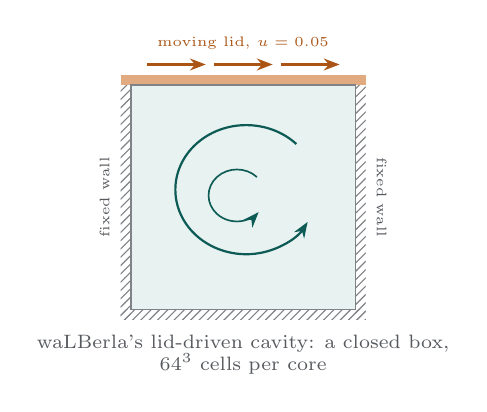
\begin{tikzpicture}
  \def\L{2.85}
  \def\t{0.13}
  % fluid
  \fill[psteal!10] (0,0) rectangle (\L,\L);
  % fixed walls (left, right, bottom): hatched
  \fill[pattern=north east lines,pattern color=psgray!80] (-\t,-\t) rectangle (0,\L);
  \fill[pattern=north east lines,pattern color=psgray!80] (\L,-\t) rectangle (\L+\t,\L);
  \fill[pattern=north east lines,pattern color=psgray!80] (-\t,-\t) rectangle (\L+\t,0);
  % the lid
  \fill[psorange!55] (-\t,\L) rectangle (\L+\t,\L+\t);
  \draw[psgray!80] (0,0) rectangle (\L,\L);
  \foreach \x in {0.2,1.05,1.9}
    \draw[arr,psorange!85!black,very thick] (\x,\L+0.26) -- ++(0.75,0);
  \node[font=\tiny,text=psorange!85!black,anchor=south] at (\L/2,\L+0.33) {moving lid, $u = 0.05$};
  % the rotating flow
  \draw[arr,psteal!75!black,thick] (2.1,2.1) arc[start angle=45,end angle=330,x radius=0.9,y radius=0.82];
  \draw[arr,psteal!75!black] (1.6,1.68) arc[start angle=45,end angle=320,x radius=0.36,y radius=0.33];
  \node[font=\tiny,text=psgray!90!black,rotate=90,anchor=south] at (-\t-0.02,\L/2) {fixed wall};
  \node[font=\tiny,text=psgray!90!black,rotate=-90,anchor=south] at (\L+\t+0.02,\L/2) {fixed wall};
  \node[lbl,anchor=north] at (\L/2,-0.2) {waLBerla's lid-driven cavity: a closed box,\\$64^3$ cells per core};
\end{tikzpicture}

    \column{0.57\textwidth}
    \centering\resizebox{!}{4.1cm}{% Slide 3: the two halves of an LBM time step, drawn in 2D (9 directions) for readability.
% The real model, D3Q19, is 3D with 19 directions.
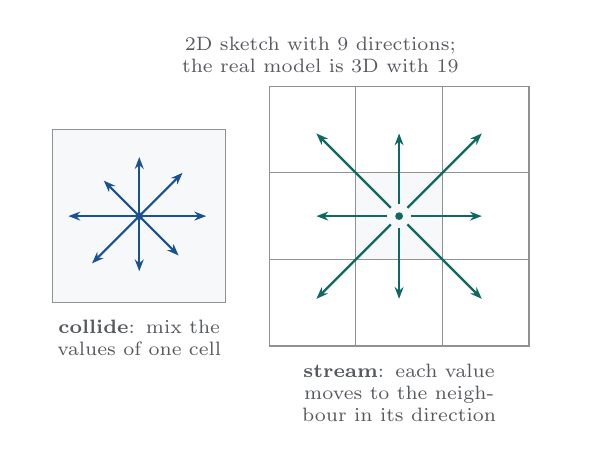
\begin{tikzpicture}[
    pdf/.style={-{Stealth[length=1.5mm]},thick,draw=psblue!85!black},
    mv/.style={-{Stealth[length=1.5mm]},thick,draw=psteal!85!black}]
  % ---- collide: one cell, one value per direction (arrow length = value)
  \draw[psgray!70,fill=codebg] (0,0.55) rectangle (2.2,2.75);
  \coordinate (c) at (1.1,1.65);
  \foreach \dx/\dy/\l in {1/0/0.85, 1/1/0.55, 0/1/0.75, -1/1/0.45, -1/0/0.9, -1/-1/0.6, 0/-1/0.7, 1/-1/0.5} {
    \draw[pdf] (c) -- ++({\dx*\l},{\dy*\l});
  }
  \fill[psblue!85!black] (c) circle (1.4pt);
  \node[lbl,anchor=north,text width=26mm] at (1.1,0.45) {\textbf{collide}: mix the values of one cell};

  % ---- stream: each value moves to the neighbour in its direction
  \begin{scope}[xshift=2.75cm]
    \foreach \i in {0,1,2} \foreach \j in {0,1,2}
      \draw[psgray!70,fill=white] (\i*1.1,\j*1.1) rectangle ++(1.1,1.1);
    \fill[codebg] (1.1,1.1) rectangle ++(1.1,1.1);
    \draw[psgray!70] (1.1,1.1) rectangle ++(1.1,1.1);
    \coordinate (s) at (1.65,1.65);
    \foreach \dx/\dy in {1/0, 1/1, 0/1, -1/1, -1/0, -1/-1, 0/-1, 1/-1}
      \draw[mv,shorten <=1.5mm] (s) -- ++({\dx*1.05},{\dy*1.05});
    \fill[psteal!85!black] (s) circle (1.4pt);
    \node[lbl,anchor=north,text width=33mm] at (1.65,-0.1) {\textbf{stream}: each value moves to the neighbour in its direction};
  \end{scope}
  \node[lbl,anchor=south,text width=60mm] at (3.4,3.35) {2D sketch with 9 directions; the real model is 3D with 19};
\end{tikzpicture}
}
  \end{columns}
  \vspace{1mm}
  \begin{itemize}\small
    \item A closed box of fluid whose lid moves. \term{waLBerla} simulates it with the \term{lattice Boltzmann
          method} (LBM): each cell stores 19 numbers (\term{D3Q19}).
    \item We measure \term{throughput} in \term{MLUP/s}: how many million cells are updated per second.
  \end{itemize}
  \takeaway{Per cell and time step: 19 loads, about 200 arithmetic operations, 23 stores.}
\end{frame}

% -----------------------------------------------------------------------------
%  The two films, unchanged from presentation6 (sources there: laptop x86 AVX, upstream pystencils; K1, the
%  verified presentation4 executable; agreement 1.2e-14 energy, 5e-15 of the lid speed, 42 frames).
\begin{frame}{The flow we compute}
  \vspace{1mm}
  \begin{columns}[T,onlytextwidth]
    \column{0.49\textwidth}
    \centering
    \movie[loop]{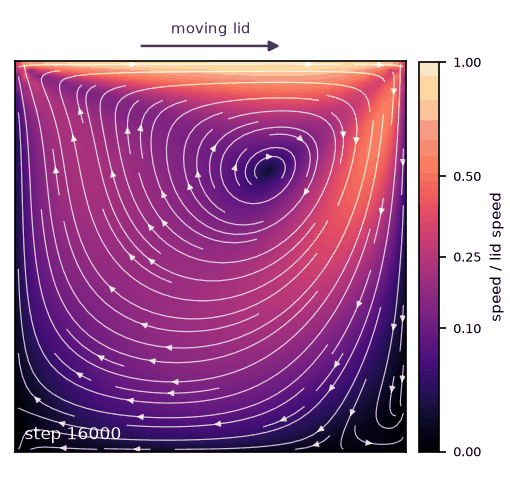
\includegraphics[height=4.4cm]{figures/cavity-movie/frame-41.png}}{figures/cavity-movie/cavity.avi}\par
    \vspace{1mm}
    {\small\textbf{Laptop}: x86 with AVX vectors\par}
    \column{0.49\textwidth}
    \centering
    \movie[loop]{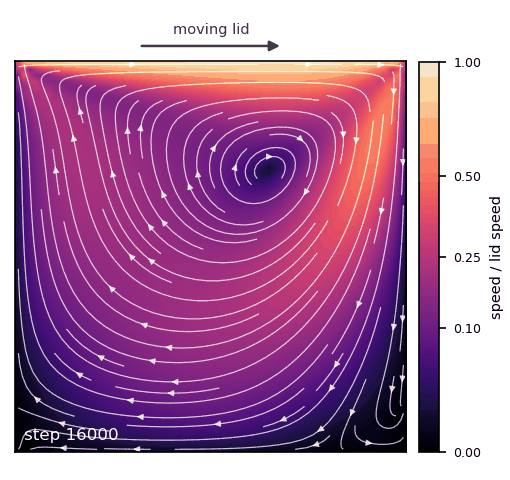
\includegraphics[height=4.4cm]{figures/cavity-movie-board/frame-41.png}}{figures/cavity-movie-board/cavity.avi}\par
    \vspace{1mm}
    {\small\textbf{K1}: RISC-V with our RVV code\par}
  \end{columns}
  \vspace{1.5mm}
  {\scriptsize\color{psgray}Middle plane of a $64^3$ box, f64, from rest to 16\,000 steps. Colour: speed; lines:
  direction of the flow. Click to play.\par}
\end{frame}

% -----------------------------------------------------------------------------
\subsection{Running on many cores}
\begin{frame}{Running on many cores}
  \vspace{3mm}
  \centering% Slide "How waLBerla splits the work" (report r02, section "The block-structured domain" and its
% figure blockforest.tex). The benchmark uses a uniform block grid with one 64^3 block per MPI
% process and one process per core; no threads (WALBERLA_BUILD_WITH_OPENMP is OFF). The halo
% exchange copies locally between blocks of the same process and sends MPI messages otherwise;
% with one process the periodic domain makes the block its own neighbour (a local copy).
% Inside a block, x is the fastest index (fzyx layout), so one RVV instruction covers VLEN / 32 (f32)
% neighbouring cells of a row: 8 on the K1 (VLEN 256, solid box), 4 on the SG2044 (VLEN 128, dashed box).
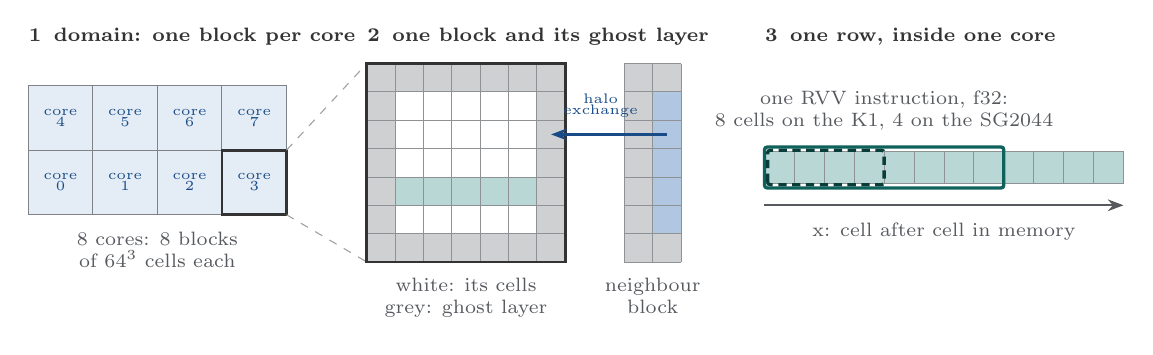
\begin{tikzpicture}[
    cell/.style={draw=psgray!70,line width=0.3pt},
    ttl/.style={font=\scriptsize\bfseries,anchor=south west,text=black!80,inner sep=0pt}]
  % ---- 1: the domain, one block per core ------------------------------------------
  \def\bs{0.82}
  \node[ttl] at (0,2.75) {1\enspace domain: one block per core};
  \foreach \i in {0,...,3} \foreach \j in {0,1} {
    \pgfmathtruncatemacro{\c}{\i+4*\j}
    \fill[psblue!12] (\i*\bs,0.6+\j*\bs) rectangle ++(\bs,\bs);
    \draw[psgray!80] (\i*\bs,0.6+\j*\bs) rectangle ++(\bs,\bs);
    \node[font=\tiny,text=psblue!80!black,align=center] at (\i*\bs+0.5*\bs,0.6+\j*\bs+0.5*\bs) {core\\[-2pt]\c};
  }
  \draw[black!80,line width=1pt] (3*\bs,0.6) rectangle ++(\bs,\bs);
  \node[lbl,anchor=north] at (2*\bs,0.5) {8 cores: 8 blocks\\of $64^3$ cells each};
  %   zoom onto the block of panel 2
  \draw[psgray!60,dashed] (4*\bs,0.6+\bs) -- (4.3,2.52);
  \draw[psgray!60,dashed] (4*\bs,0.6) -- (4.3,0);

  % ---- 2: one block, its ghost layer and the halo exchange -------------------------
  \begin{scope}[shift={(4.3,0)}]
    \def\s{0.36}
    \node[ttl] at (0,2.75) {2\enspace one block and its ghost layer};
    \fill[psgray!30] (0,0) rectangle (7*\s,7*\s);
    \fill[white] (\s,\s) rectangle (6*\s,6*\s);
    \fill[psteal!30] (\s,2*\s) rectangle (6*\s,3*\s);            % one row (panel 3)
    \draw[cell,step=\s] (0,0) grid (7*\s,7*\s);
    \draw[black!80,line width=1pt] (0,0) rectangle (7*\s,7*\s);
    \node[lbl,anchor=north] at (3.5*\s,-0.08) {white: its cells\\grey: ghost layer};
    %   the east neighbour, another process: its first interior column is the border slice
    \begin{scope}[shift={(7*\s+0.75,0)}]
      \fill[psgray!30] (0,0) rectangle (2*\s,7*\s);
      \fill[psblue!35] (\s,\s) rectangle (2*\s,6*\s);
      \draw[cell,step=\s] (0,0) grid (2*\s,7*\s);
      \node[lbl,anchor=north] at (\s,-0.08) {neighbour\\block};
    \end{scope}
    \draw[arr,psblue!80!black,thick] (7*\s+0.75+1.5*\s,4.5*\s) -- (6.5*\s,4.5*\s);
    \node[font=\tiny,text=psblue!80!black,align=center,anchor=south] at (7*\s+0.45,4.75*\s)
      {halo\\[-2pt]exchange};
  \end{scope}

  % ---- 3: one row of cells inside one core ----------------------------------------
  \begin{scope}[shift={(9.35,0)}]
    \def\w{0.38}
    \node[ttl] at (0,2.75) {3\enspace one row, inside one core};
    \foreach \k in {0,...,11} {
      \fill[psteal!30] (\k*\w,1.0) rectangle ++(\w,0.4);
      \draw[cell] (\k*\w,1.0) rectangle ++(\w,0.4);
    }
    \draw[psteal!80!black,line width=1.2pt,rounded corners=1pt] (0,0.94) rectangle (8*\w,1.46);
    \draw[psteal!50!black,line width=1.2pt,rounded corners=1pt,densely dashed] (0.04,0.98) rectangle (4*\w,1.42);
    \node[lbl,anchor=south] at (4*\w,1.55) {one RVV instruction, f32:\\8 cells on the K1, 4 on the SG2044};
    \draw[arr] (0,0.72) -- (12*\w,0.72);
    \node[lbl,anchor=north] at (6*\w,0.62) {x: cell after cell in memory};
  \end{scope}
\end{tikzpicture}


  \vspace{4mm}
  \raggedright
  \begin{itemize}\small
    \item Each core runs one \term{MPI} process with one block of $64^3$ cells.
    \item After each step, neighbouring blocks exchange their border cells (\term{halo exchange}).
  \end{itemize}
  \takeaway{More cores give a larger box (\term{weak scaling}). Ideally, $N$ cores give $N$ times the MLUP/s.}
\end{frame}

% -----------------------------------------------------------------------------
%  figures/time-step.tex has the sources (order of the time loop, the three timers of the app).
\begin{frame}{What one time step does}
  \vspace{1.5mm}
  \centering% Slide "What one time step does" (new in presentation7-v2, so that "wall pass" is defined before the time-share
% plots use it). The order in the benchmark's time loop (submodules/walberla/apps/benchmarks/SweepgenLdcCPU/
% SweepgenLdcCPU.cpp:33-35 and 210-256): StreamCollide (the kernel), then the halo exchange (streamPullSync, or
% aaPullSync / aaPushSync), then NoSlip and UBB on the wall links (the wall pass). The app times the three parts
% separately: t_bulk, t_comm, t_bc (line 361), which are the three colours of the time-share plots.
% Bottom: the wall rule (bounce-back) in 2D. NoSlip: a value that would stream into a fixed wall comes back in the
% opposite direction. UBB (the lid): the same, plus a small change that carries the lid's speed into the fluid.
% The wall pass is generated for Target.GenericCPU in every variant (SweepgenLdcCPU.py:28-29, 135-141).
% Segment widths are only a sketch; the measured shares are on the "where the time goes" slides.
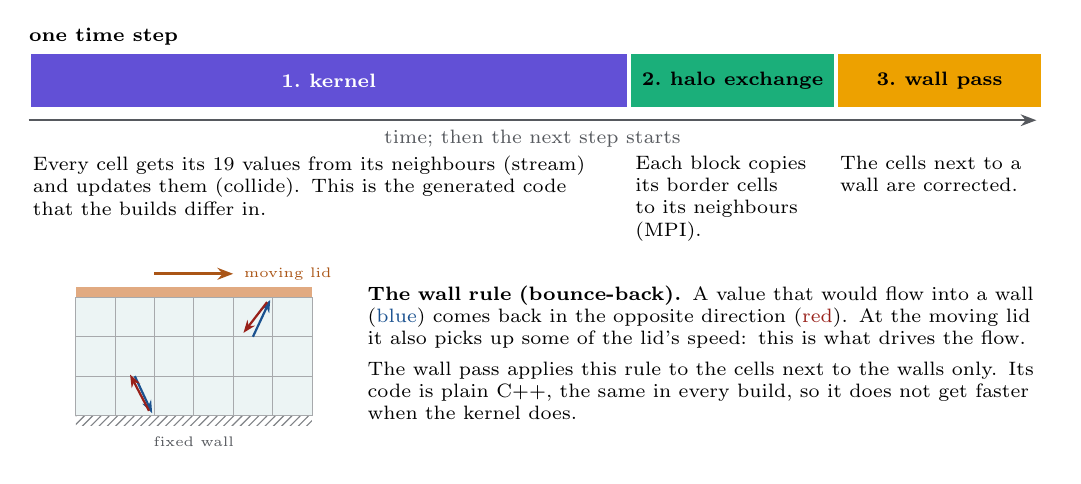
\begin{tikzpicture}[x=1cm,y=1cm]
  \tikzset{seg/.style={draw=white,line width=0.8pt,minimum height=7mm,inner sep=2pt,font=\scriptsize,
             align=center,anchor=west},
           dsc/.style={font=\scriptsize,align=left,anchor=north west,inner sep=0pt,text width=#1},
           cellb/.style={draw=psgray!55,line width=0.3pt,fill=psteal!8}}
  % ---- one time step: three parts, one after the other -------------------------------
  \node[font=\scriptsize\bfseries,anchor=south west,inner sep=0pt] at (0,0.45) {one time step};
  \node[seg,fill=ckernel,text=white,minimum width=7.6cm] (k) at (0,0) {\textbf{1.\ kernel}};
  \node[seg,fill=ccomm,minimum width=2.6cm] (h) at (k.east) {\textbf{2.\ halo exchange}};
  \node[seg,fill=cwall,minimum width=2.6cm] (w) at (h.east) {\textbf{3.\ wall pass}};
  \draw[arr] (0,-0.5) -- (12.8,-0.5) node[pos=0.5,below,lbl] {time; then the next step starts};
  \node[dsc=7.3cm] at (0.05,-0.95) {Every cell gets its 19 values from its neighbours (stream) and updates them
    (collide). This is the generated code that the builds differ in.};
  \node[dsc=2.5cm] at (7.7,-0.95) {Each block copies its border cells to its neighbours (MPI).};
  \node[dsc=2.5cm] at (10.3,-0.95) {The cells next to a wall are corrected.};

  % ---- the wall rule: bounce-back ------------------------------------------------------
  \begin{scope}[shift={(0.6,-4.25)}]
    \def\s{0.5}
    %   fixed wall below, the lid above, fluid cells between
    \fill[pattern=north east lines,pattern color=psgray!80] (0,-0.13) rectangle (6*\s,0);
    \fill[psorange!55] (0,3*\s) rectangle (6*\s,3*\s+0.13);
    \foreach \i in {0,...,5} \foreach \j in {0,1,2} \draw[cellb] (\i*\s,\j*\s) rectangle ++(\s,\s);
    \draw[arr,psorange!85!black,very thick] (1.0,3*\s+0.3) -- ++(1.0,0)
      node[right,font=\tiny,text=psorange!85!black] {moving lid};
    \node[font=\tiny,text=psgray!90!black,anchor=north] at (3*\s,-0.15) {fixed wall};
    %   a value heading into the fixed wall comes back the other way
    \draw[-{Stealth[length=1.6mm]},thick,psblue!85!black] (1.5*\s,0.5*\s+0.25) -- (1.5*\s+0.22,0.03);
    \draw[-{Stealth[length=1.6mm]},thick,psred!85!black] (1.5*\s+0.18,0.06) -- (1.5*\s-0.06,0.5*\s+0.27);
    %   and one heading into the lid
    \draw[-{Stealth[length=1.6mm]},thick,psblue!85!black] (4.5*\s,2.5*\s-0.25) -- (4.5*\s+0.22,3*\s-0.03);
    \draw[-{Stealth[length=1.6mm]},thick,psred!85!black] (4.5*\s+0.18,3*\s-0.06) -- (4.5*\s-0.12,2.5*\s-0.2);
  \end{scope}
  \node[dsc=8.7cm] at (4.3,-2.6) {%
    \textbf{The wall rule (bounce-back).} A value that would flow into a wall
    (\textcolor{psblue!85!black}{blue}) comes back in the opposite direction
    (\textcolor{psred!85!black}{red}). At the moving lid it also picks up some of the lid's speed: this is what
    drives the flow.\\[3pt]
    The wall pass applies this rule to the cells next to the walls only. Its code is plain C++, the same in
    every build, so it does not get faster when the kernel does.};
\end{tikzpicture}%

  \takeaway{Each time step has three parts: the \term{kernel}, the \term{halo exchange} and the \term{wall pass}.
    Only the kernel is generated as vector code.}
\end{frame}

% -----------------------------------------------------------------------------
\subsection{RISC-V vectors}
\begin{frame}{RISC-V vectors: each chip chooses its register width}
  \begin{columns}[T,onlytextwidth]
    \column{0.52\textwidth}
    \vspace{4mm}
    \centering\resizebox{0.98\linewidth}{!}{% Slide "RISC-V vectors: the register width differs between chips". The RVV specification lets each chip
% choose its register width VLEN; the instructions are the same. K1: VLEN 256 (SpacemiT X60), SG2044: VLEN 128
% (C920v2), both measured from the vlenb register (presentation4 / notes7 builds: CMake "RISC-V VLEN").
% The intrinsic type vfloat32m1_t means "one register of f32": 8 lanes on the K1, 4 on the SG2044.
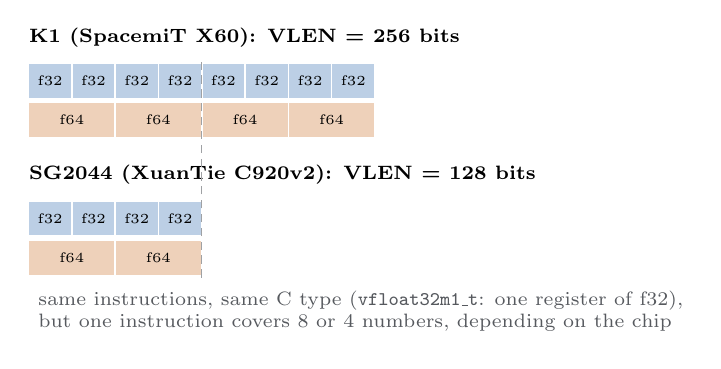
\begin{tikzpicture}
  \def\w{0.55}
  \foreach \row/\n/\lab/\y in {0/8/{K1 (SpacemiT X60): VLEN = 256 bits}/0, 1/4/{SG2044 (XuanTie C920v2): VLEN = 128 bits}/-1.75} {
    \node[font=\scriptsize\bfseries,anchor=south west,inner sep=0pt] at (0,\y+0.42) {\lab};
    \foreach \k in {1,...,\n}
      \node[draw=white,line width=0.6pt,minimum height=4.5mm,inner sep=0pt,font=\tiny,fill=psblue!30,
        minimum width=\w cm] at (\k*\w-\w/2,\y) {f32};
    \pgfmathtruncatemacro{\h}{\n/2}
    \foreach \k in {1,...,\h}
      \node[draw=white,line width=0.6pt,minimum height=4.5mm,inner sep=0pt,font=\tiny,fill=psorange!30,
        minimum width=2*\w cm] at (\k*2*\w-\w,\y-0.5) {f64};
  }
  \draw[psgray!60,densely dashed] (4*\w,-2.5) -- (4*\w,0.3);
  \node[lbl,anchor=north west,align=left] at (0,-2.55)
    {same instructions, same C type (\code{vfloat32m1\_t}: one register of f32),\\but one instruction
     covers 8 or 4 numbers, depending on the chip};
\end{tikzpicture}
}
    \column{0.46\textwidth}
    \vspace{2mm}
    \begin{itemize}\small
      \item \term{RVV 1.0}
      \item K1: VLEN = 256 bits.\\ SG2044: VLEN = 128 bits.
      \item One PyStencil backend for both, VLEN is set in compile-time.
    \end{itemize}
  \end{columns}
  \takeaway{Targetting max speedup of \sx{8} on the K1 and \sx{4} on the SG2044 (f32).\\
    For f64 the limits are \sx{4} and \sx{2}.}
\end{frame}

% =============================================================================
\section[Code for two widths]{Code for two vector widths}
\subsection{From Python to a running program}

\begin{frame}{From Python to a running program}
  \vspace{1mm}
  \centering% From source to a running simulation (report r02, chapter "Code Generation" and its figure
% build-flow.tex). CMake configures; during "make", CMake runs the Python generator scripts
% (sweepgen sets jit = no_jit: generate only), then compiles the generated C++ together with
% the hand-written waLBerla core. The executable runs without Python. The time loop runs the kernel, the halo
% exchange and the wall pass (generated index-list loops, Target.GenericCPU: plain C++ in every build). Everything ran on the
% board. Violet = generated code. Each column is one step; the small arrows between the
% headers carry the results from step to step (no wires across columns).
%
% With \brmarkerstrue (slide "Where each change lives") numbered markers show what we changed:
% blue = part 1, teal = part 2 (10 to 12: the last three changes, see the open-work slide).
% The markers sit on the nodes a2, g0, g2, g3, i1, i2 and cc.
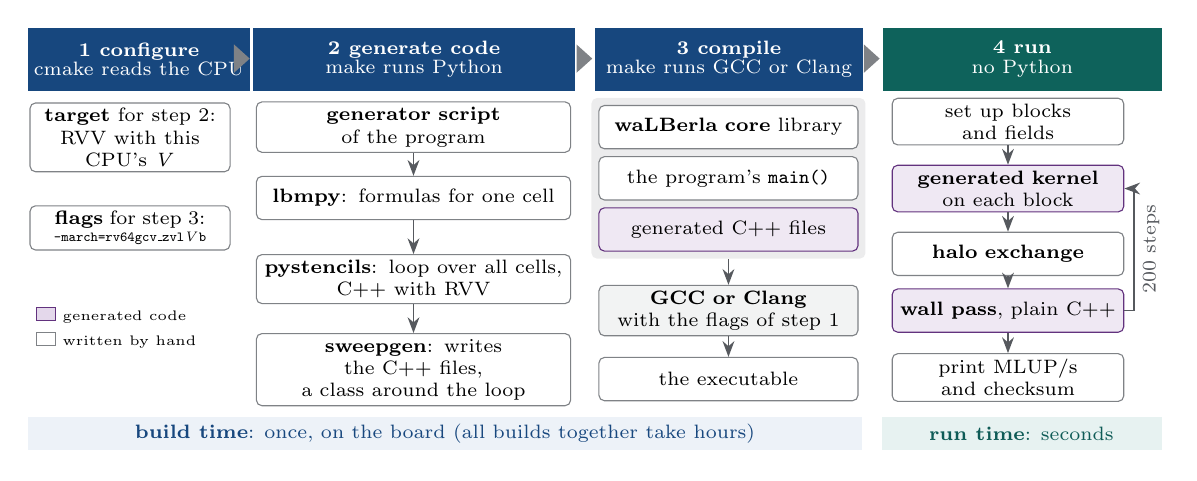
\begin{tikzpicture}[
    hdr/.style={font=\scriptsize\bfseries,text=white,align=center,inner sep=2pt,
      minimum height=8mm,anchor=north west},
    b/.style={box,font=\scriptsize,minimum height=5.5mm,inner sep=2pt,
      execute at begin node={\hyphenpenalty=10000\exhyphenpenalty=10000}},
    gen/.style={b,fill=psviolet!12,draw=psviolet!80!black},
    hdrarr/.style={fill=psgray!80},
    mk/.style={circle,text=white,font=\tiny\bfseries,inner sep=0pt,minimum size=3.7mm}]
  \ifbrmarkers\tikzset{mkl/.style={align=left}}\else\tikzset{mkl/.style={}}\fi
  % ---- column headers, with arrows from step to step --------------------------------
  \node[hdr,fill=psblue!75!black,minimum width=2.6cm] at (0,0)
    {1 configure\\[-1pt]{\mdseries cmake reads the CPU}};
  \node[hdr,fill=psblue!75!black,minimum width=4.1cm] at (2.85,0)
    {2 generate code\\[-1pt]{\mdseries make runs Python}};
  \node[hdr,fill=psblue!75!black,minimum width=3.4cm] at (7.2,0)
    {3 compile\\[-1pt]{\mdseries make runs GCC or Clang}};
  \node[hdr,fill=psteal!80!black,minimum width=3.55cm] at (10.85,0)
    {4 run\\[-1pt]{\mdseries no Python}};
  \foreach \x in {2.62,6.97,10.62}
    \fill[hdrarr] (\x,-0.22) -- ++(0.2,-0.18) -- ++(-0.2,-0.18) -- cycle;

  % ---- 1 configure: two settings for the later steps --------------------------------
  \node[b,text width=2.4cm] (a3) at (1.3,-1.4) {\textbf{target} for step 2:\\RVV with this CPU's \textit{V}};
  \node[b,text width=2.4cm,font=\tiny] (a2) at (1.3,-2.55)
    {{\scriptsize\textbf{flags} for step 3:}\\\code{-march=rv64gcv\_zvl}\textit{V}\code{b}};
  \node[anchor=north west,font=\tiny,align=left,inner sep=0pt] at (0.1,-3.55)
    {\tikz\fill[psviolet!20,draw=psviolet!80!black] (0,0) rectangle (2.4mm,1.6mm);\ generated code\\[3pt]
     \tikz\draw[psgray!80] (0,0) rectangle (2.4mm,1.6mm);\ written by hand};

  % ---- 2 generate: the Python tool chain ---------------------------------------------
  \node[b,text width=3.85cm] (g0) at (4.9,-1.27) {\textbf{generator script} of the program};
  \node[b,text width=3.85cm] (g1) at (4.9,-2.17) {\textbf{lbmpy}: formulas for one cell};
  \node[b,text width=3.85cm] (g2) at (4.9,-3.2) {\textbf{pystencils}: loop over all cells,\\C++ with RVV};
  \node[b,text width=3.85cm] (g3) at (4.9,-4.35) {\textbf{sweepgen}: writes the C++ files,\\a class around the loop};
  \foreach \u/\v in {g0/g1,g1/g2,g2/g3} \draw[arr] (\u) -- (\v);

  % ---- 3 compile: hand-written and generated C++ together ----------------------------
  \node[b,mkl,text width=3.15cm] (i1) at (8.9,-1.27) {\textbf{waLBerla core} library};
  \node[b,mkl,text width=3.15cm] (i2) at (8.9,-1.92) {the program's \code{main()}};
  \node[gen,text width=3.15cm] (i0) at (8.9,-2.57) {generated C++ files};
  \begin{scope}[on background layer]
    \node[fill=psgray!12,rounded corners=2pt,inner sep=2.5pt,fit=(i1)(i2)(i0)] (src) {};
  \end{scope}
  \node[b,text width=3.15cm,fill=psgray!8] (cc) at (8.9,-3.6) {\textbf{GCC or Clang}\\with the flags of step 1};
  \node[b,text width=3.15cm] (exe) at (8.9,-4.47) {the executable};
  \draw[arr] (src) -- (cc);
  \draw[arr] (cc) -- (exe);

  % ---- 4 run: set up, then the time loop (kernel, halo exchange, wall pass; notes5 F16) ----
  \node[b,text width=2.8cm] (r0) at (12.45,-1.2) {set up blocks and fields};
  \node[gen,text width=2.8cm] (r1) at (12.45,-2.05) {\textbf{generated kernel}\\on each block};
  \node[b,text width=2.8cm] (r2) at (12.45,-2.88) {\textbf{halo exchange}};
  \node[gen,text width=2.8cm] (rw) at (12.45,-3.6) {\textbf{wall pass}, plain C++};
  \node[b,text width=2.8cm] (r3) at (12.45,-4.45) {print MLUP/s and checksum};
  \draw[arr] (r0) -- (r1);
  \draw[arr] (r1) -- (r2);
  \draw[arr] (r2) -- (rw);
  \draw[arr] (rw.east) -- ++(0.12,0) |- (r1.east);
  \node[lbl,rotate=90] at (14.27,-2.82) {200 steps};
  \draw[arr] (rw) -- (r3);

  % ---- time bands ----------------------------------------------------------------------
  \fill[psblue!8] (0,-4.95) rectangle (10.6,-5.37);
  \node[font=\scriptsize,text=psblue!75!black] at (5.3,-5.16)
    {\textbf{build time}: once, on the board (all builds together take hours)};
  \fill[psteal!10] (10.85,-4.95) rectangle (14.4,-5.37);
  \node[font=\scriptsize,text=psteal!75!black] at (12.62,-5.16) {\textbf{run time}: seconds};

  % ---- markers: what we changed ------------------------------------------------------
  \ifbrmarkers
    \tikzset{mk/.append style={minimum size=3.2mm}}
    %   \brmark: on top of the box's upper border; \brmarkin: inside the box, at its right end
    \def\brmark#1#2#3#4{% node, slot (0 = rightmost), colour, number
      \node[mk,fill=#3] at ([xshift={-2.2mm-#2*3.6mm},yshift=1.3mm]#1.north east) {#4};}
    \def\brmarkin#1#2#3#4{%
      \node[mk,fill=#3] at ([xshift={-2.2mm-#2*3.6mm}]#1.east) {#4};}
    \brmark{a2}{0}{psblue}{1}   \brmark{a2}{1}{psteal}{8}
    \brmark{g0}{0}{psblue}{3}
    \brmark{g2}{0}{psblue}{2}   \brmark{g2}{1}{psteal}{5}   \brmark{g2}{2}{psteal}{12}
    \brmark{g3}{0}{psteal}{6}   \brmark{g3}{1}{psteal}{10}
    \brmarkin{i1}{0}{psteal}{11} \brmarkin{i1}{1}{psteal}{7}
    \brmarkin{i2}{0}{psteal}{9}    \brmarkin{i2}{1}{psblue}{3}
    \brmark{cc}{0}{psblue}{4}
  \fi
\end{tikzpicture}

  \vspace{1mm}
  \raggedright{\scriptsize\color{psgray}\textit{V} is the vector width in bits: 256 on the K1, 128 on the SG2044.\par}
  \takeaway{Python runs only while the program is built. The program that runs is plain C++.}
\end{frame}

% -----------------------------------------------------------------------------
\subsection{What we added}
\begin{frame}{What we added, and the builds we compare}
  \vspace{2mm}
  \centering% Slide "What we added": the four pieces that were missing on RISC-V (report r02, chapter "What
% Was Missing"): compiler flags in the waLBerla build, an RVV target in pystencils, a compile-time
% check for the register width (it checks the compiler flags, not the hardware: notes5 F10), and a benchmark program that asks for vector code.
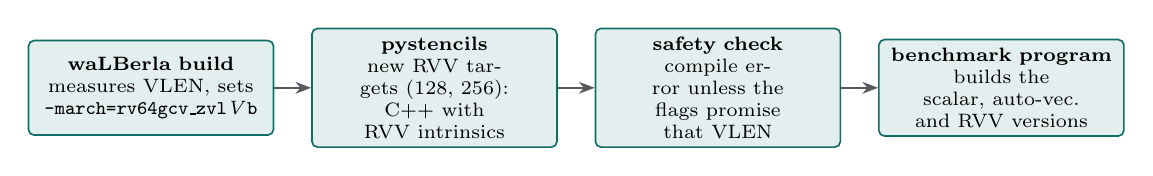
\begin{tikzpicture}[
    pc/.style={added,text width=29mm,minimum height=12mm,font=\scriptsize,align=center}]
  \def\dx{3.6}
  \node[pc] (a1) at (0,0)     {\textbf{waLBerla build}\\measures VLEN, sets\\\code{-march=rv64gcv\_zvl}\textit{V}\code{b}};
  \node[pc] (a2) at (\dx,0)   {\textbf{pystencils}\\new RVV targets (128, 256):\\C++ with RVV intrinsics};
  \node[pc] (a3) at (2*\dx,0) {\textbf{safety check}\\compile error unless the\\flags promise that VLEN};
  \node[pc] (a4) at (3*\dx,0) {\textbf{benchmark program}\\builds the scalar, auto-vec.\\and RVV versions};
  \foreach \u/\v in {a1/a2,a2/a3,a3/a4} \draw[arr] (\u) -- (\v);
\end{tikzpicture}


  \vspace{4mm}
  {\footnotesize\renewcommand{\arraystretch}{1.12}
  \begin{tabular}{@{}lll@{}}
    \toprule
    \textbf{build} & \textbf{kernel} & \textbf{compiler flags}\\
    \midrule
    plain scalar & plain C++ & \code{-march=rv64gc}: no vector instructions\\
    auto-vectorized & plain C++ & \code{-march=rv64gcv\_zvl}\textit{V}\code{b}: the compiler may vectorize\\
    best scalar & plain C++ with \term{CSE} and \term{in-place} update & \code{-march=rv64gc}\\
    \textbf{RVV} & \textbf{RVV intrinsics}, with options: in place, & \code{-march=rv64gcv\_zvl}\textit{V}\code{b}\\
    & \hspace{1em}\term{software prefetch}, \term{split loop} & \\
    \bottomrule
  \end{tabular}\par}

  \vspace{2mm}
  {\scriptsize\color{psgray}CSE: repeated parts of the formulas are computed once. The other options are explained
  later. 11 builds in total, each with GCC~14.2 and Clang (18.1 on the K1, 17 on the SG2044), \code{-O3}, in f32
  and f64.\par}
\end{frame}

% -----------------------------------------------------------------------------
%  figures/backends.tex has the sources (the platform classes and targets of the pystencils fork).
\begin{frame}{pystencils: one backend for each instruction set}
  \vspace{2mm}
  \centering\resizebox{\textwidth}{!}{% Slide "pystencils: one backend for each instruction set" (new in presentation7-v2; answers the todo "how many
% backends, and is the RVV backend duplicated for VLEN 128 / 256 or per microarchitecture").
% Source: the fork submodules/pystencils/src/pystencils/: backend/platforms/ has one platform class per family:
% generic_cpu.py (GenericCpu), x86.py (X86VectorCpu; X86VectorArch = SSE, AVX, AVX512 ...), neon.py (NeonCpu),
% sve.py (SveCpu), rvv.py (RvvCpu), cuda.py, hip.py, sycl.py (+ generic_gpu.py). codegen/target.py: X86_SSE,
% X86_AVX, X86_AVX512, ARM_NEON, ARM_SVE, RISCV_RVV128, RISCV_RVV256 (RISCV_RVV = RISCV_RVV256), CUDA, HIP, SYCL.
% rvv.py: class RvvCpu(GenericVectorCpu), __init__(ctx, vlen), SUPPORTED_VLENS = (128, 256): one class, the
% width is a parameter. grep for X60 / C920 / SpacemiT / Sophgo in the package finds only comments (examples of
% machines), no code that depends on the chip.
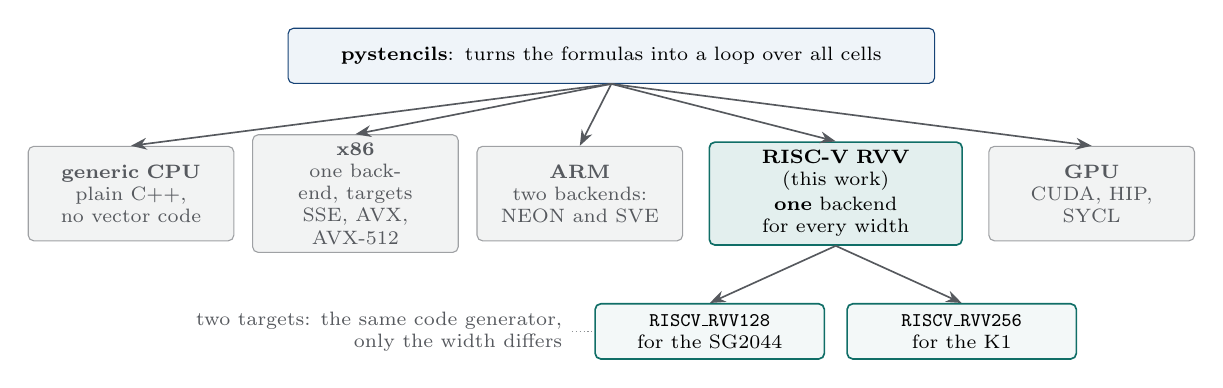
\begin{tikzpicture}
  \tikzset{be/.style={box,quiet,text width=24mm,minimum height=12mm,font=\scriptsize},
           ours/.style={box,added,text width=30mm,minimum height=12mm,font=\scriptsize},
           tg/.style={box,added,fill=psteal!5,text width=27mm,font=\scriptsize,minimum height=7mm}}
  \node[box,info,text width=80mm,font=\scriptsize] (ps) at (6.1,1.75)
    {\textbf{pystencils}: turns the formulas into a loop over all cells};
  \node[be] (gen) at (0,0) {\textbf{generic CPU}\\plain C++,\\no vector code};
  \node[be] (x86) at (2.85,0) {\textbf{x86}\\one backend, targets\\SSE, AVX, AVX-512};
  \node[be] (arm) at (5.7,0) {\textbf{ARM}\\two backends:\\NEON and SVE};
  \node[ours] (rvv) at (8.95,0) {\textbf{RISC-V RVV} (this work)\\[1pt]\textbf{one} backend\\for every width};
  \node[be] (gpu) at (12.2,0) {\textbf{GPU}\\CUDA, HIP,\\SYCL};
  \foreach \b in {gen,x86,arm,rvv,gpu} \draw[arr] (ps.south) -- (\b.north);
  \node[tg] (t128) at (7.35,-1.75) {\code{RISCV\_RVV128}\\for the SG2044};
  \node[tg] (t256) at (10.55,-1.75) {\code{RISCV\_RVV256}\\for the K1};
  \draw[arr] (rvv.south) -- (t128.north);
  \draw[arr] (rvv.south) -- (t256.north);
  \node[lbl,anchor=east,align=right] (two) at (5.6,-1.75) {two targets: the same code generator,\\only the width differs};
  \draw[psgray!70,densely dotted] (two.east) -- (t128.west);
\end{tikzpicture}%
}

  \vspace{1mm}
  \raggedright
  \begin{itemize}\small
    \item A \term{backend} turns the loop into code for one instruction set. The \term{target} chooses the
          backend and its options, for example the vector width.
    \item We added one RVV backend for every width, as x86 has one backend for SSE, AVX and AVX-512. Nothing in
          it is written for a particular chip: the X60 and the C920v2 get the same generator.
  \end{itemize}
  \takeaway{One RVV backend, two targets: \code{RISCV\_RVV128} and \code{RISCV\_RVV256}.}
\end{frame}

% -----------------------------------------------------------------------------
\begin{frame}{How the build chooses the target}
  \vspace{4mm}
  \centering\resizebox{\textwidth}{!}{% Slide "One code generator for 128- and 256-bit vectors": how the register width travels from the build
% machine into the generated code (docs/notes7/rvv-vlen128-plan-opus5.5.md, section 3; implementation in the
% forks: waLBerla cmake/compileroptions/RiscvVlen.cmake (try_run of a probe that reads the vlenb register),
% GNU.cmake / Clang.cmake (-march=rv64gcv_zvl<V>b), sweepgen build_config.riscv_vlen -> Target.RISCV_RVV<V>;
% pystencils codegen/target.py (RISCV_RVV128, RISCV_RVV256), backend/platforms/rvv.py, include/
% pystencils_runtime/rvv_vlen128.hpp (sets PYSTENCILS_RVV_VLEN 128, includes rvv.hpp), rvv.hpp (#error unless
% __riscv_v_min_vlen >= PYSTENCILS_RVV_VLEN; VLEN 256 code includes rvv.hpp directly, default 256).
% __riscv_v_min_vlen is what the -march flag promises (zvl128b -> 128), not what the hardware has.
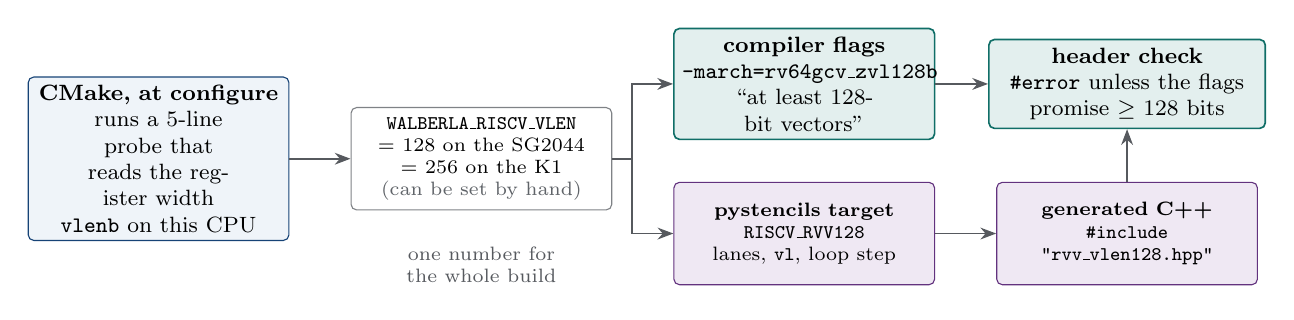
\begin{tikzpicture}[
    st/.style={box,text width=31mm,minimum height=13mm,font=\scriptsize,align=center},
    hw/.style={st,info},
    gen/.style={st,fill=psviolet!12,draw=psviolet!80!black},
    cc/.style={st,added}]
  \node[hw] (probe) at (0,0) {\textbf{CMake, at configure}\\runs a 5-line probe that\\reads the register width\\\code{vlenb} on this CPU};
  \node[st] (v) at (4.1,0) {\code{WALBERLA\_RISCV\_VLEN}\\= 128 on the SG2044\\= 256 on the K1\\{\color{psgray}(can be set by hand)}};
  \node[cc] (flags) at (8.2,0.95) {\textbf{compiler flags}\\\code{-march=rv64gcv\_zvl128b}\\``at least 128-bit vectors''};
  \node[gen] (tgt) at (8.2,-0.95) {\textbf{pystencils target}\\\code{RISCV\_RVV128}\\lanes, \code{vl}, loop step};
  \node[gen] (code) at (12.3,-0.95) {\textbf{generated C++}\\\code{\#include "rvv\_vlen128.hpp"}};
  \node[cc,text width=33mm] (guard) at (12.3,0.95) {\textbf{header check}\\\code{\#error} unless the flags\\promise $\ge$ 128 bits};
  \draw[arr] (probe) -- (v);
  \draw[arr] (v.east) -- ++(0.25,0) |- (flags.west);
  \draw[arr] (v.east) -- ++(0.25,0) |- (tgt.west);
  \draw[arr] (tgt) -- (code);
  \draw[arr] (flags) -- (guard);
  \draw[arr] (code) -- (guard);
  \node[lbl,anchor=north] at (4.1,-1.0) {one number for\\the whole build};
\end{tikzpicture}
}

  \vspace{4mm}
  \raggedright
  \begin{itemize}\small
    \item CMake measures the width of the chip it runs on. That one number sets both the pystencils target and the
          compiler flags.
    \item At 256 bits the generator writes the same code as before this work. So the K1 results still hold.
  \end{itemize}
  \takeaway{The build measures the width once. The generated code and the compiler flags both follow from it.}
\end{frame}

% -----------------------------------------------------------------------------
%  Generated on the laptop with the fork (pystencils 78afe1ff): a 2D 4-point stencil, f32,
%  Target.RISCV_RVV256 and RISCV_RVV128, cpu.vectorize.enable, assume_inner_stride_one, default_dtype float32
%  (the generator script is recorded in the progress file). Lines shortened with "...".
\begin{frame}[fragile]{The generated code at the two widths}
  \vspace{1mm}
  {\small A small stencil in f32, generated for each target:\par}
  \vspace{2mm}
  \begin{columns}[T,onlytextwidth]
    \column{0.49\textwidth}
    {\scriptsize\bfseries \code{RISCV\_RVV256} (K1)\par}
    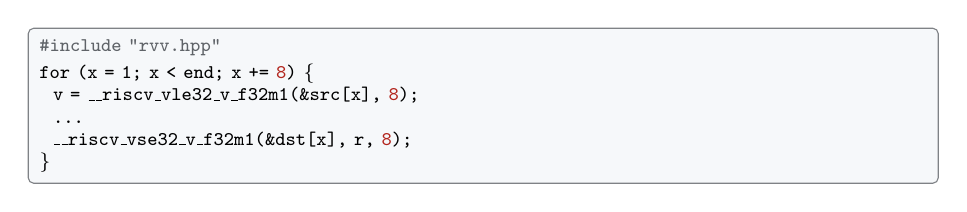
\begin{tikzpicture}
      \node[codebox,text width=0.93\textwidth] {%
        \textcolor{psgray}{\#include "rvv.hpp"}\\[2pt]
        for (x = 1; x < end; x += \textcolor{psred}{\textbf{8}}) \{\\
        \ \ v = \_\_riscv\_vle32\_v\_f32m1(\&src[x], \textcolor{psred}{\textbf{8}});\\
        \ \ ...\\
        \ \ \_\_riscv\_vse32\_v\_f32m1(\&dst[x], r, \textcolor{psred}{\textbf{8}});\\
        \}};
    \end{tikzpicture}
    \column{0.49\textwidth}
    {\scriptsize\bfseries \code{RISCV\_RVV128} (SG2044)\par}
    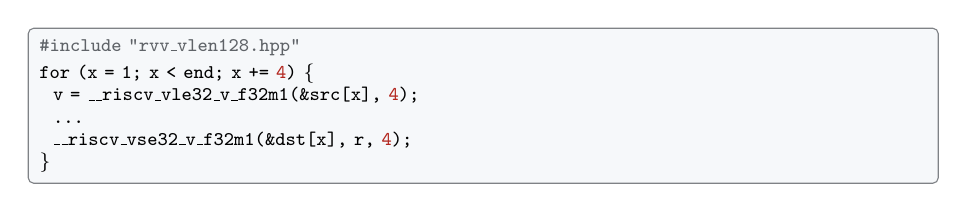
\begin{tikzpicture}
      \node[codebox,text width=0.93\textwidth] {%
        \textcolor{psgray}{\#include "rvv\_vlen128.hpp"}\\[2pt]
        for (x = 1; x < end; x += \textcolor{psred}{\textbf{4}}) \{\\
        \ \ v = \_\_riscv\_vle32\_v\_f32m1(\&src[x], \textcolor{psred}{\textbf{4}});\\
        \ \ ...\\
        \ \ \_\_riscv\_vse32\_v\_f32m1(\&dst[x], r, \textcolor{psred}{\textbf{4}});\\
        \}};
    \end{tikzpicture}
  \end{columns}
  \vspace{3mm}
  \begin{itemize}\small
    \item \code{vle32} loads and \code{vse32} stores. The last argument (\term{vl}) is how many numbers one
          instruction handles.
    \item The type \code{f32m1} means one register of f32 numbers: 8 on the K1, 4 on the SG2044.
  \end{itemize}
  \takeaway{Only two numbers change between the widths: \code{vl} and the loop step.}
\end{frame}

% -----------------------------------------------------------------------------
\subsection{Safety and correctness}
%  docs/notes7/rvv-vlen128-progress-opus5.5.md, step 1: test_rvv_qemu.py (six kernels on a 5 x 23 grid,
%  cross-compiled -static, qemu-riscv64 -cpu rv64,v=true,vlen=N, compared with the same kernels for GenericCPU);
%  control: VLEN-256 code at vlen 128 gets 30-55 of 115 cells wrong per kernel and a wrong sum; 154 RVV tests pass.
\begin{frame}{A wrong width gives wrong results, so it stops the build}
  \vspace{2mm}
  \begin{itemize}
    \item \textbf{The danger.} 256-bit code on a 128-bit chip handles 4 numbers per instruction but steps by 8.
          Half of the cells are never updated. There is no crash and no warning.
    \item \textbf{A test.} In a RISC-V emulator set to 128 bits, 256-bit code got 30 to 55 of 115 cells wrong in
          each of six kernels.
    \item \textbf{The protection.} The generated file includes a header that stops the compiler unless the
          compiler flags promise at least the width of the code.
    \item The build sets these flags from the width it measured on the chip.
  \end{itemize}
  \takeaway{If the code and the flags do not match, the program is not built.}
\end{frame}

% -----------------------------------------------------------------------------
%  K1: board-logs/k1/board/verify-*.log (presentation4); SG2044: verify-*.log of run 20261122-214637 (job
%  8565). Errors: the largest max|drho|, max|du| against reference.npz over all four reference cases and all 11
%  builds per log (slide_data.py). Energies of the timed runs: largest relative spread of the 11 builds, per
%  compiler, precision and core count. Energy = sum over all cells of ux^2 + uy^2 + uz^2, summed in double
%  (SweepgenLdcCPU.cpp:281-307). sha256: of each benchmark executable; the timing script (presentation4/6
%  all.sh) refuses to start unless every executable's sha256 appears in the verify log.
\begin{frame}{How we check the results}
  \vspace{2mm}
  \begin{itemize}\small
    \item A separate NumPy script computes the same flow, as our \term{reference}.
    \item Every build is matched against the \term{reference} cell by cell.
    \item The programs we time are the same executable files that passed this check: their \term{sha256}
          checksums are equal.
    \item Each run ends by printing one number for the whole flow, the \term{energy}: the sum of
          $u_x^2 + u_y^2 + u_z^2$ over all cells ($u$ is the flow velocity). All 11 builds print the same energy,
          up to rounding.
  \end{itemize}
  \vspace{3mm}
  \centering
  {\footnotesize\renewcommand{\arraystretch}{1.15}
  \begin{tabular}{@{}lccc@{}}
    \toprule
    & \textbf{programs checked} & \textbf{largest error vs reference} & \textbf{energy: largest relative difference}\\
    & & f64 / f32 & \textbf{between the 11 builds}, f64 / f32\\
    \midrule
    K1 & \nv{kone:verified} & $\nv{kone:referr:f64}$ / $\nv{kone:referr:f32}$
      & $\nv{kone:energyspread:f64}$ / $\nv{kone:energyspread:f32}$\\
    SG2044 & \nv{sg:verified} & $\nv{sg:referr:f64}$ / $\nv{sg:referr:f32}$
      & $\nv{sg:energyspread:f64}$ / $\nv{sg:energyspread:f32}$\\
    \bottomrule
  \end{tabular}\par}
  \takeaway{Every build on both machines computes the reference flow, up to rounding
    ($2\cdot 10^{-16}$ is the rounding error of f64).}
\end{frame}

% =============================================================================
\section[The kernel]{The kernel and its memory traffic}
\subsection{Updating one cell}

\begin{frame}{The stencil: the cells needed to update one cell}
  \begin{columns}[T,onlytextwidth]
    \column{0.53\textwidth}
    \vspace{4mm}
    \centering% Slide "The stencil: the cells needed to update one cell" (new in presentation5), drawn in 3D.
% D3Q19 in lbmpy's order, the order of the generated code (direction c_i = (c_x, c_y, c_z)):
%   0 C (0,0,0)   1 N (0,1,0)   2 S (0,-1,0)  3 W (-1,0,0)  4 E (1,0,0)   5 T (0,0,1)   6 B (0,0,-1)
%   7 NW (-1,1,0) 8 NE (1,1,0)  9 SW (-1,-1,0) 10 SE (1,-1,0) 11 TN (0,1,1) 12 TS (0,-1,1) 13 TW (-1,0,1)
%   14 TE (1,0,1) 15 BN (0,1,-1) 16 BS (0,-1,-1) 17 BW (-1,0,-1) 18 BE (1,0,-1)
% Pull: the new f_i of cell x is the old f_i of the cell x - c_i. Checked against the generated StreamCollide
% (SweepgenLdcCPU_scalar_cse, build/presentation4-x86/gcc-f32, gen/SweepgenLdcCPU.cpp:44-130): f_3 is read at
% ctr_0 + 1, f_4 at ctr_0 - 1, f_1 at ctr_1 - 1, f_5 at ctr_2 - 1, f_9 at (ctr_0 + 1, ctr_1 + 1),
% f_14 at (ctr_0 - 1, ctr_2 - 1), f_17 at (ctr_0 + 1, ctr_2 + 1).
% Each dot is a cell; it is labelled with the value the update takes from it, and its arrow points the way
% that value moves (c_i), into the cell in the middle. Axes: i = +x (east), j = +y (north, into the page),
% k = +z (top); ctr_0, ctr_1, ctr_2 in the generated code.
% Overlays: 1 the 3 x 3 x 3 cells around the cell and the cell itself, 2 the 6 face neighbours (f_4 in orange:
% the example of the text), 3 the 12 edge neighbours, 4 the 8 corners, which D3Q19 does not read.
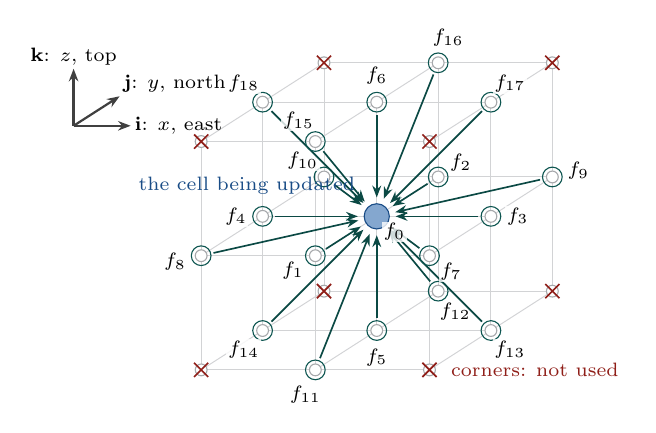
\begin{tikzpicture}[x={(1.45cm,0cm)},y={(0.78cm,0.5cm)},z={(0cm,1.45cm)}]
  \tikzset{
    lat/.style={draw=psgray!28,line width=0.35pt},
    pt/.style={circle,draw=psgray!55,fill=white,inner sep=0pt,minimum size=1.5mm},
    me/.style={circle,draw=psblue!80!black,fill=psblue!55,inner sep=0pt,minimum size=3.2mm},
    nb/.style={circle,draw=psteal!70!black,inner sep=0pt,minimum size=2.5mm},
    %   #1: the overlay on which this group appears (strong colour there, light afterwards)
    grp/.style={nb,visible on=<#1->,alt=<#1>{fill=psteal!75}{fill=psteal!30}},
    mv/.style={-{Stealth[length=1.5mm]},semithick,draw=psteal!60!black},
    fl/.style={font=\scriptsize,inner sep=0.6pt,fill=white,fill opacity=0.8,text opacity=1},
    ax/.style={-{Stealth[length=1.6mm]},thick,draw=black!75},
    axl/.style={font=\scriptsize,inner sep=1pt},
  }
  \coordinate (C) at (0,0,0);
  % ---- the 27 cells around and including the cell, with faint lattice lines (back to front)
  \foreach \a in {-1,0,1} \foreach \b in {-1,0,1} {
    \draw[lat] (-1,\a,\b) -- (1,\a,\b);
    \draw[lat] (\a,-1,\b) -- (\a,1,\b);
    \draw[lat] (\a,\b,-1) -- (\a,\b,1);
  }
  \foreach \b in {1,0,-1} \foreach \a in {-1,0,1} \foreach \c in {-1,0,1}
    \node[pt] at (\a,\b,\c) {};

  %   \nbr{overlay}{a}{b}{c}{i}: the neighbour at (a,b,c) sends f_i into the cell
  \newcommand{\nbr}[5]{%
    \coordinate (P) at (#2,#3,#4);
    \draw[mv,visible on=<#1->] ($(P)!1.6mm!(C)$) -- ($(C)!2.4mm!(P)$);
    \node[grp=#1] at (P) {};
    \node[fl,visible on=<#1->] at ($(P)!-3.4mm!(C)$) {$f_{#5}$};}
  %   back plane (y = +1) first, so the front is drawn on top
  \nbr{2}{0}{1}{0}{2}
  \nbr{3}{1}{1}{0}{9}   \nbr{3}{-1}{1}{0}{10}  \nbr{3}{0}{1}{-1}{12}  \nbr{3}{0}{1}{1}{16}
  \nbr{2}{1}{0}{0}{3}   \nbr{2}{0}{0}{-1}{5}   \nbr{2}{0}{0}{1}{6}
  \nbr{3}{1}{0}{-1}{13} \nbr{3}{-1}{0}{-1}{14} \nbr{3}{1}{0}{1}{17}   \nbr{3}{-1}{0}{1}{18}
  \nbr{2}{0}{-1}{0}{1}
  \nbr{3}{1}{-1}{0}{7}  \nbr{3}{-1}{-1}{0}{8}  \nbr{3}{0}{-1}{-1}{11} \nbr{3}{0}{-1}{1}{15}
  %   f_4 last and in orange on overlay 2: it moves east, so it comes from the west neighbour
  \coordinate (P) at (-1,0,0);
  \draw[mv,visible on=<2->,alt=<2>{draw=psorange!90!black,very thick}{}] ($(P)!1.6mm!(C)$) -- ($(C)!2.4mm!(P)$);
  \node[nb,visible on=<2->,alt=<2>{fill=psorange!70,draw=psorange!90!black}{fill=psteal!30}] at (P) {};
  \node[fl,visible on=<2->] at ($(P)!-3.4mm!(C)$) {$f_{4}$};
  % ---- the cell itself; f_0 stays
  \node[me] at (C) {};
  \node[fl,font=\scriptsize\bfseries,anchor=north west] at ([xshift=0.6mm,yshift=-0.6mm]C) {$f_0$};
  \node[font=\scriptsize,text=psblue!80!black,anchor=south east,visible on=<1>] at ([xshift=-1.5mm,yshift=1.5mm]C)
    {the cell being updated};

  % ---- 4: the 8 corners are not part of D3Q19
  \foreach \a in {-1,1} \foreach \b in {-1,1} \foreach \c in {-1,1}
    \draw[psred!80!black,semithick,visible on=<4->] ([shift={(-0.9mm,-0.9mm)}]\a,\b,\c) -- ++(1.8mm,1.8mm)
      ([shift={(-0.9mm,0.9mm)}]\a,\b,\c) -- ++(1.8mm,-1.8mm);
  \node[font=\scriptsize,text=psred!80!black,anchor=west,visible on=<4->] at ([xshift=1.5mm]1,-1,-1) {corners: not used};

  % ---- axes: the unit vectors i, j, k of x, y, z, in a corner of their own
  \begin{scope}[shift={(-3.85cm,1.15cm)}]
    \draw[ax] (0,0,0) -- (0.5,0,0) node[axl,anchor=west] {$\mathbf{i}$: $x$, east};
    \draw[ax] (0,0,0) -- (0,0.75,0) node[axl,anchor=south west] {$\mathbf{j}$: $y$, north};
    \draw[ax] (0,0,0) -- (0,0,0.5) node[axl,anchor=south] {$\mathbf{k}$: $z$, top};
  \end{scope}
\end{tikzpicture}

    \column{0.45\textwidth}
    \vspace{1mm}
    \begin{itemize}\small
      \item Each cell stores 19 values, $f_0$ to $f_{18}$: the fluid moving in 19 directions.
      \item<2-> In each time step, every value moves one cell along its direction. The kernel fetches it from
            the neighbour it comes from. Example: $f_4$ moves east, so it comes from the west neighbour.
      \item<4-> The \term{stencil}: the cell itself, 6 face neighbours and 12 edge neighbours. The 8 corners
            are not used.
    \end{itemize}
  \end{columns}
  \takeaway{To update one cell, the kernel reads 19 values: one from the cell itself and 18 from neighbours.}
\end{frame}

% -----------------------------------------------------------------------------
\begin{frame}{How the 19 values are stored in memory}
  \centering% Slide "How the 19 values are stored in memory" (new in presentation5; redrawn after the user's reviews).
% The small array is the same 3 x 3 x 3 cube as on the stencil slide (the cell in the middle and its 26
% neighbours), drawn with its three planes pulled apart, every cell numbered with its place in memory, and the
% same numbers in one contiguous strip of memory: x fastest, then y, then z (waLBerla's layout fzyx). The cell
% in the middle is 13; its 6 face neighbours are 13 -+ 1 (x), 13 -+ 3 (y), 13 -+ 9 (z). Colours as on the
% stencil slide: the cell being updated in blue, its neighbours in teal.
% Then one row of our real arrays, colour-coded: 1 ghost cell + 64 cells of the block + 1 ghost cell + 2 values
% of padding = 68 values. Real arrays: waLBerla's v8 fields, layout fzyx (submodules/walberla
% include/walberla/v8/memory/Field.hpp: 215-252): allocated shape (64 + 2 ghost) per axis, linearization order
% x, y, z, f (x fastest, f = the direction slowest), the x line padded to the host alignment
% (BufferSystem.hpp:441-452; 16 B on the board, so a row of 66 floats becomes 68, notes3 progress "Loop 3").
% Strides in f32 values: x 1, y 68, z 68 * 66 = 4488, f 4488 * 66 = 296208, i.e. +4 B, +272 B, +17 952 B
% (about 18 KB), +1 184 832 B (about 1.2 MB). (f64: 66, 4356, 287496 values.) The index is the one of the
% generated vector kernels (explicit_*: x stride 1; gen/SweepgenLdcCPU.cpp:94-96 of explicit_cse, gcc-f32),
% here for f_4:
%   _data_f[ctr_0 + ctr_1 * _stride_f_1 + ctr_2 * _stride_f_2 + 4LL * _stride_f_3]
% presentation7-v2: the text says that the numbers are cell positions in the array of ONE value (f_4), not the
% values f_0..f_18 (user's review).
% Overlays: 1 the empty cube and memory; 2 the first row (x fastest); 3 the other rows of plane 0 (then y);
% 4 planes 1 and 2 (then z); 5 the neighbours of cell 13 and the index x + 3y + 9z; 6 one row of our real
% arrays (ghost cells, padding) and the index of the generated code.
\begin{tikzpicture}[x=1cm,y=1cm]
  \tikzset{
    cb/.style={draw=psgray!60,line width=0.3pt},
    num/.style={font=\scriptsize,inner sep=0pt},
    me/.style={draw=psblue!80!black,fill=psblue!50,line width=1.1pt},
    nb/.style={draw=psteal!70!black,fill=psteal!40,line width=1.1pt},
    hop/.style={-{Stealth[length=1.5mm]},semithick,draw=psteal!60!black},
    lb/.style={font=\scriptsize,text=psgray!90!black,inner sep=1pt},
    tl/.style={font=\tiny,text=psgray!90!black,inner sep=1pt},
    ob/.style={font=\scriptsize,text=psteal!60!black,inner sep=1pt},
    ax/.style={-{Stealth[length=1.4mm]},semithick,draw=black!75},
    ghost/.style={cb,fill=psgray!50},
    inner/.style={cb,fill=psblue!22},
    pad/.style={draw=psgray!80,densely dashed,line width=0.3pt,fill=white},
    pin/.style={draw=psgray!80,line width=0.4pt},
  }
  \path (-1.45,-2.05) rectangle (12.95,3.05);   % the same size on every overlay
  %   the cube in 3D: x step (0.62, 0), y step (0.38, 0.24); planes z = 0, 1, 2 at heights 0.35, 1.33, 2.31
  \def\cx{0.62}\def\cyx{0.38}\def\cyy{0.24}
  \def\base#1{\ifcase#1 0.35\or 1.33\or 2.31\fi}
  %   \cellat{x}{y}{z}{options}: the parallelogram of one cell; \cellc: its centre
  \def\cellat#1#2#3#4{\draw[#4] ({\cx*#1+\cyx*#2},{\base{#3}+\cyy*#2}) -- ++(\cx,0) -- ++(\cyx,\cyy) -- ++(-\cx,0) -- cycle;}
  \def\cellc#1#2#3{({\cx*(#1+0.5)+\cyx*(#2+0.5)},{\base{#3}+\cyy*(#2+0.5)})}
  %   the three planes are one block: dashed lines join their corners
  \foreach \px/\py in {0/0, 1.86/0, 3.0/0.72, 1.14/0.72}
    \draw[densely dashed,psgray!45] (\px,0.35+\py) -- (\px,2.31+\py);
  %   cells: white, then coloured and numbered from the overlay that reaches them
  %   (orange = plane z = 0, violet = plane z = 1, grey = plane z = 2; darker = larger y)
  \foreach \z in {0,1,2} \foreach \y in {0,1,2} \foreach \x in {0,1,2} {
    \pgfmathtruncatemacro\n{\x+3*\y+9*\z}
    \pgfmathtruncatemacro\s{ifthenelse(\n<3,2,ifthenelse(\n<9,3,4))}
    \pgfmathtruncatemacro\sh{12+13*\y}
    \ifcase\z \def\hue{psorange}\or\def\hue{psviolet}\or\def\hue{psgray}\fi
    \cellat{\x}{\y}{\z}{cb,fill=white}
    \cellat{\x}{\y}{\z}{cb,fill=\hue!\sh,visible on=<\s->}
    \node[num,visible on=<\s->] at \cellc{\x}{\y}{\z} {\n};
  }
  %   5: the cell in the middle (13) and its 6 face neighbours, coloured as on the stencil slide
  \begin{scope}[visible on=<5->]
    \foreach \x/\y/\z/\n in {1/2/1/16, 0/1/1/12, 2/1/1/14, 1/0/1/10, 1/1/0/4, 1/1/2/22} {
      \cellat{\x}{\y}{\z}{nb}
      \node[num] at \cellc{\x}{\y}{\z} {\n};
    }
    \cellat{1}{1}{1}{me}
    \node[num,font=\scriptsize\bfseries] at \cellc{1}{1}{1} {13};
  \end{scope}
  %   axis labels on the cube
  \foreach \x in {0,1,2} \node[tl,anchor=north] at ({\cx*(\x+0.5)},0.33) {\x};
  \node[tl,anchor=north east] at (0,0.33) {$x$:};
  \foreach \y in {0,1,2} \node[tl,anchor=west] at ({3*\cx+\cyx*(\y+0.5)+0.03},{0.35+\cyy*(\y+0.5)}) {\y};
  \node[tl,anchor=west] at ({3*\cx+\cyx*3+0.03},{0.35+\cyy*3+0.02}) {$y$};
  \foreach \z in {0,1,2} \node[tl,anchor=east,fill=white] at ({\cyx*1.5-0.06},{\base{\z}+\cyy*1.5}) {$z = \z$};
  %   the unit vectors, as on the stencil slide
  \begin{scope}[shift={(-1.35,1.0)}]
    \draw[ax] (0,0) -- (0.5,0) node[tl,text=black,anchor=west] {$\mathbf{i}$ ($x$)};
    \draw[ax] (0,0) -- (0.34,0.23) node[tl,text=black,anchor=south west] {$\mathbf{j}$ ($y$)};
    \draw[ax] (0,0) -- (0,0.5) node[tl,text=black,anchor=south west] {$\mathbf{k}$ ($z$)};
  \end{scope}

  % ================= memory: one strip with the same numbers (overlays 1-5) ==========================
  \def\sw{0.42}\def\smx{0.5}
  \node[lb,anchor=east,align=right] at (\smx-0.06,-0.32) {memory:\\array of $f_4$};
  \node[tl,anchor=south east,visible on=<1-5>] at (\smx+27*\sw,-0.12) {addresses grow $\rightarrow$};
  \foreach \k in {0,...,26} {
    \pgfmathtruncatemacro\r{\k/3}
    \pgfmathtruncatemacro\y{mod(\r,3)}
    \pgfmathtruncatemacro\z{\k/9}
    \pgfmathtruncatemacro\s{ifthenelse(\k<3,2,ifthenelse(\k<9,3,4))}
    \pgfmathtruncatemacro\sh{12+13*\y}
    \ifcase\z \def\hue{psorange}\or\def\hue{psviolet}\or\def\hue{psgray}\fi
    \draw[cb,fill=white,visible on=<1-5>] ({\smx+\k*\sw},-0.5) rectangle ++(\sw,0.36);
    \draw[cb,fill=\hue!\sh,visible on=<\s-5>] ({\smx+\k*\sw},-0.5) rectangle ++(\sw,0.36);
    \node[num,visible on=<\s-5>] at ({\smx+(\k+0.5)*\sw},-0.32) {\k};
  }
  \foreach \r in {0,...,8} {
    \pgfmathtruncatemacro\y{mod(\r,3)}
    \pgfmathtruncatemacro\s{ifthenelse(\r<1,2,ifthenelse(\r<3,3,4))}
    \node[tl,anchor=north,visible on=<\s-5>] at ({\smx+(3*\r+1.5)*\sw},-0.52) {row $y = \y$};
  }
  \foreach \z/\hue/\s in {0/psorange/3, 1/psviolet/4, 2/psgray/4}
    \draw[decorate,decoration={brace,amplitude=3pt,mirror},\hue!90!black,visible on=<\s-5>]
      ({\smx+9*\z*\sw},-0.73) -- ({\smx+9*(\z+1)*\sw},-0.73)
      node[midway,below=1pt,font=\scriptsize,text=\hue!80!black] {plane $z = \z$};
  %   5: the neighbours of cell 13 in memory
  \begin{scope}[visible on=<5>]
    \foreach \k in {4,10,12,14,16,22} {
      \draw[nb] ({\smx+\k*\sw},-0.5) rectangle ++(\sw,0.36);
      \node[num] at ({\smx+(\k+0.5)*\sw},-0.32) {\k};
    }
    \draw[me] ({\smx+13*\sw},-0.5) rectangle ++(\sw,0.36);
    \node[num,font=\scriptsize\bfseries] at ({\smx+13.5*\sw},-0.32) {13};
    \foreach \k/\b/\p/\t in {14/80/0.5/{+1}, 16/35/0.55/{+3}, 22/18/0.55/{+9}}
      \draw[hop] ({\smx+13.5*\sw+0.05},-0.12) to[bend left=\b] node[above,ob,pos=\p] {$\t$} ({\smx+(\k+0.5)*\sw},-0.12);
    \foreach \k/\b/\p/\t in {12/80/0.5/{-1}, 10/35/0.55/{-3}, 4/18/0.55/{-9}}
      \draw[hop] ({\smx+13.5*\sw-0.05},-0.12) to[bend right=\b] node[above,ob,pos=\p] {$\t$} ({\smx+(\k+0.5)*\sw},-0.12);
  \end{scope}

  % ================= 6: one row of our real arrays, colour-coded ====================================
  \def\rsw{0.16}
  \begin{scope}[visible on=<6>]
    \foreach \k in {0,...,67} {
      \ifnum\k=0 \def\st{ghost}\else\ifnum\k<65 \def\st{inner}\else\ifnum\k=65 \def\st{ghost}\else
        \def\st{pad}\fi\fi\fi
      \draw[\st] ({\smx+\k*\rsw},-0.5) rectangle ++(\rsw,0.36);
    }
    \draw[decorate,decoration={brace,amplitude=3pt},psgray!90!black]
      ({\smx},-0.1) -- ({\smx+68*\rsw},-0.1)
      node[midway,above=2pt,font=\scriptsize] {one row of our real arrays: 68 values, or 272 bytes in f32};
    \draw[decorate,decoration={brace,amplitude=3pt,mirror},psblue!80!black]
      ({\smx+\rsw+0.02},-0.56) -- ({\smx+65*\rsw-0.02},-0.56)
      node[midway,below=2pt,font=\scriptsize,text=psblue!80!black] {the 64 cells of the block in this row};
    \draw[pin] ({\smx+0.5*\rsw},-0.5) -- ++(0,-0.3) node[lb,text=black,anchor=north] {ghost cell};
    \draw[pin] ({\smx+65.5*\rsw},-0.5) -- ++(0,-0.3) node[lb,text=black,anchor=north east] {ghost cell};
    \draw[pin] ({\smx+67*\rsw},-0.5) -- ++(0,-0.3) node[lb,text=black,anchor=north west] {padding};
  \end{scope}

  % ================= what the overlays say ==========================================================
  \node[anchor=north west,text width=9.0cm,align=left,font=\scriptsize,inner sep=0pt] at (3.9,3.05) {%
    \begin{itemize}\setlength{\itemsep}{0.5pt}
      \item Take the array of one of the 19 values, say $f_4$, and imagine it has only $3 \times 3 \times 3$
            cells: the 27 cells around one cell from the last slide.
      \item Each number is the position of a cell in this array. It is \textbf{not} one of the values $f_0$ to
            $f_{18}$: each of those has an array like this one.
      \item<2-> $x$ changes fastest: the 3 cells of a row are stored side by side.
      \item<3-> Then $y$: the rows of a plane follow each other.
      \item<4-> Then $z$: the planes follow each other.
      \item<5-> So for the cell in the middle (number 13), the neighbours in $x$ are 1 position away, in $y$
            3 positions (one row), and in $z$ 9 positions (one plane).
    \end{itemize}};

  % ================= the index: first for the small array, then for ours ============================
  \begin{scope}[visible on=<5->,every node/.style={font=\ttfamily\scriptsize,inner sep=0pt,anchor=base west}]
    \node (t0) at (-1.05,-1.47) {\alt<6>{f4[z][y][x]\ \ is\ \ \_data\_f[\ }{cell[z][y][x]\ \ is\ \ a[\ }\mbox{}};
    \node[base right=0pt of t0] (t1) {x};
    \node[base right=0pt of t1] (p1) {\alt<6>{\ +\ }{\ \ \ +\ \ \ }\mbox{}};
    \node[base right=0pt of p1] (t2) {\alt<6>{y*\_stride\_f\_1}{3*y}};
    \node[base right=0pt of t2] (p2) {\alt<6>{\ +\ }{\ \ \ +\ \ \ }\mbox{}};
    \node[base right=0pt of p2] (t3) {\alt<6>{z*\_stride\_f\_2}{9*z}};
    \node[base right=0pt of t3] (p3) {\alt<6>{\ +\ \mbox{}}{}};
    \node[base right=0pt of p3] (t4) {\alt<6>{4*\_stride\_f\_3}{}};
    \node[base right=0pt of t4] (t5) {\ ]};
  \end{scope}
  \begin{scope}[on background layer]
    \node[draw=psgray!80,fill=codebg,rounded corners=2pt,inner sep=3pt,fit=(t0)(t5),visible on=<5->] (ix) {};
  \end{scope}
  \node[lb,anchor=west,align=left,visible on=<5->] at ([xshift=2mm]ix.east)
    {\alt<6>{generated code; strides in\\f32: 68, 4\,488 and 296\,208}%
            {small array: 3 positions per\\row, 9 per plane}};
  %   braces under the terms
  \def\brc#1#2{\draw[decorate,decoration={brace,amplitude=2.5pt,mirror},psteal!70!black]
      ([yshift=-1.3mm]#1.south west) -- ([yshift=-1.3mm]#1.south east) node[midway,below=1.5pt,ob] {#2};}
  \only<5>{\brc{t1}{$+1$}\brc{t2}{$+3$}\brc{t3}{$+9$}}
  \only<6>{\brc{t1}{$+4$\,B}\brc{t2}{$+272$\,B}\brc{t3}{$+18$\,KB}\brc{t4}{$+1.2$\,MB: $f_5$}}
\end{tikzpicture}%


  \raggedright
  \uncover<6->{\footnotesize Each of the 19 values has its own 3D array like this one (\term{layout fzyx}).
  A \term{ghost layer} of one cell surrounds the block and holds the neighbour's values.\par}
  \takeaway{Neighbours in $x$ are next to each other. The 19 values of one cell are 1.2\,MB apart (f32).}
\end{frame}

% -----------------------------------------------------------------------------
\begin{frame}{The kernel code: updating one cell, step by step}
  \vspace{-2.5mm}
  \centering% Slide "The kernel in code: one cell update, load by load" (new in presentation5).
% Left: the generated StreamCollide, shortened to its shape (SweepgenLdcCPU_scalar_cse and _explicit_cse,
% build/presentation4-x86/gcc-f32/apps/benchmarks/SweepgenLdcCPU/_gen/*/gen/SweepgenLdcCPU.cpp:41-345):
%   src[i][z][y][x] = _data_f[x + y * _stride_f_1 + z * _stride_f_2 + i * _stride_f_3]  (previous slide),
%   dst = _data_f_tmp (AB pattern: a second set of 19 arrays), rho_out = _data_rho, u_out = _data_u (3 arrays).
% In the real code the 19 loads are spread over the formulas (e.g. xi_5 = f3(x+1) + f9(x+1,y+1) + f17(x+1,z+1)),
% the collide part is about 200 operations, and the stores are 19 + 4 lines; the offsets shown are the real
% ones (f_4 at ctr_0 - 1, f_1 at ctr_1 - 1, f_5 at ctr_2 - 1; see stencil-d3q19.tex). The last overlay
% shows the RVV build (explicit_*): ctr_0 += L and every load/store a vector of L consecutive values, L = VLEN / 32
% in f32: 8 on the K1 (VLEN 256), 4 on the SG2044 (VLEN 128); f64 half of that (vle32 / vse32 stand for
% __riscv_vle32_v_f32m1 / __riscv_vse32_v_f32m1; presentation7: L instead of 8, the last 4 slots drawn light).
% presentation7-v2 (user's review: "too much to understand", "the code is too abstract"): the loads and stores
% are written with the flat index of the layout slide, with the real f32 strides of our arrays (row 68 values,
% plane 68 * 66 = 4488, array 4488 * 66 = 296208; field-layout.tex), and the 9 overlays became 5:
% 1 the loops, 2 the loads (4 shown, 15 more), 3 collide (no memory access), 4 the stores, 5 the same with vectors.
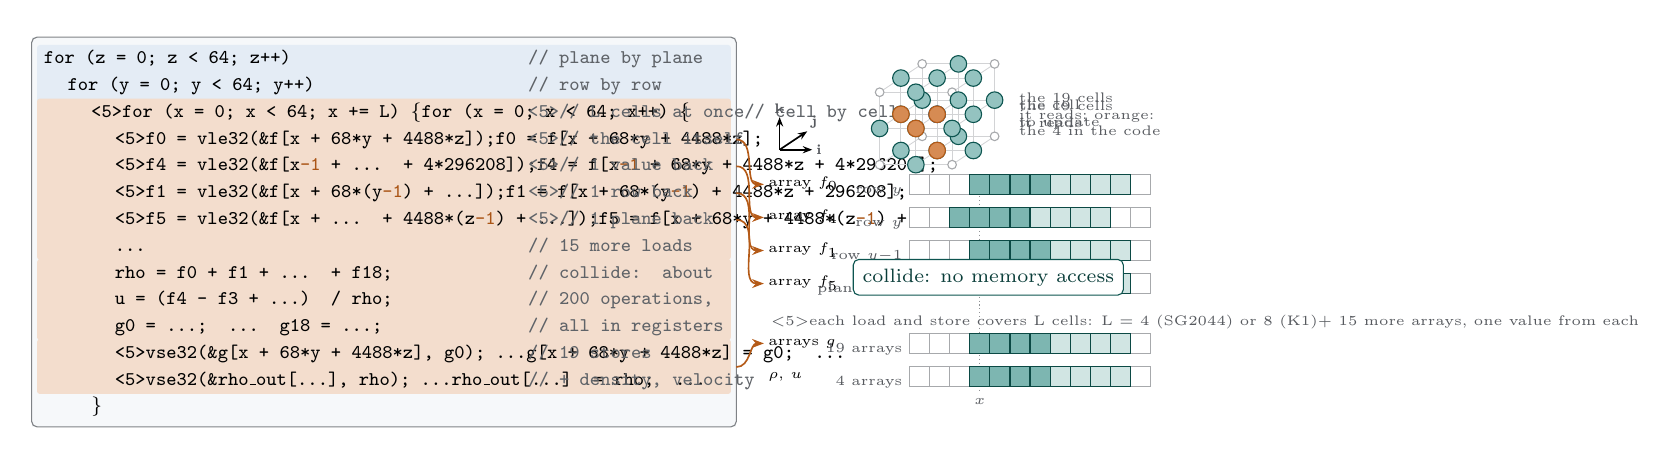
\begin{tikzpicture}[x=1cm,y=1cm]
  \tikzset{
    kl/.style={font=\ttfamily\scriptsize,inner sep=0pt,anchor=base west},
    kc/.style={kl,text=psgray},
    hl/.style={fill=psorange!22,rounded corners=1pt},
    hlb/.style={fill=psblue!12,rounded corners=1pt},
    sl/.style={draw=psgray!55,fill=white,line width=0.3pt},
    cur/.style={draw=psorange!90!black,fill=psorange!60,line width=0.4pt},
    done/.style={draw=psteal!70!black,fill=psteal!35,line width=0.4pt},
    vec/.style={draw=psteal!60!black,fill=psteal!55,line width=0.4pt},
    ln/.style={-{Stealth[length=1.5mm]},semithick,draw=psorange!90!black},
    lb/.style={font=\tiny,text=psgray!90!black,inner sep=1pt},
  }
  \path (-0.2,-5.0) rectangle (14.2,0.12);      % the same size on every overlay
  \def\ly{0.34}                                 % line pitch
  \def\ke#1{\textcolor{psorange!85!black}{#1}}  % a neighbour offset in the code

  % ================= the code ==================================================================
  \fill[codebg] (-0.15,0.0) rectangle (8.8,-4.95);
  \draw[psgray!80,rounded corners=2pt] (-0.15,0.0) rectangle (8.8,-4.95);
  %   line highlights (behind the text)
  \fill[hlb,visible on=<1>] (-0.08,-3*\ly-0.11) rectangle (8.73,-1*\ly+0.24);
  \fill[hl,visible on=<2>] (-0.08,-8*\ly-0.11) rectangle (8.73,-4*\ly+0.24);
  \fill[hl,visible on=<3>] (-0.08,-11*\ly-0.11) rectangle (8.73,-9*\ly+0.24);
  \fill[hl,visible on=<4>] (-0.08,-13*\ly-0.11) rectangle (8.73,-12*\ly+0.24);
  \fill[hl,visible on=<5>] (-0.08,-7*\ly-0.11) rectangle (8.73,-3*\ly+0.24);
  \fill[hl,visible on=<5>] (-0.08,-13*\ly-0.11) rectangle (8.73,-12*\ly+0.24);
  %   \kline{line}{indent}{code}{comment}; comments start at 6.15
  \def\kline#1#2#3#4{\node[kl] (L#1) at (#2*0.3,-#1*\ly) {#3}; \node[kc] at (6.15,-#1*\ly) {#4};}
  \kline{1}{0}{for (z = 0; z < 64; z++)}{// plane by plane}
  \kline{2}{1}{for (y = 0; y < 64; y++)}{// row by row}
  \kline{3}{2}{\alt<5>{for (x = 0; x < 64; x += L) \{}{for (x = 0; x < 64; x++) \{}}%
              {\alt<5>{// L cells at once}{// cell by cell}}
  \kline{4}{3}{\alt<5>{f0 = vle32(\&f[x + 68*y + 4488*z]);}{f0 = f[x + 68*y + 4488*z];}}%
              {\alt<5>{}{// the cell itself}}
  \kline{5}{3}{\alt<5>{f4 = vle32(\&f[x\ke{-1} + ... + 4*296208]);}{f4 = f[x\ke{-1} + 68*y + 4488*z + 4*296208];}}%
              {\alt<5>{}{// 1 value back}}
  \kline{6}{3}{\alt<5>{f1 = vle32(\&f[x + 68*(y\ke{-1}) + ...]);}{f1 = f[x + 68*(y\ke{-1}) + 4488*z + 296208];}}%
              {\alt<5>{}{// 1 row back}}
  \kline{7}{3}{\alt<5>{f5 = vle32(\&f[x + ... + 4488*(z\ke{-1}) + ...]);}{f5 = f[x + 68*y + 4488*(z\ke{-1}) + 5*296208];}}%
              {\alt<5>{}{// 1 plane back}}
  \kline{8}{3}{...}{// 15 more loads}
  \kline{9}{3}{rho = f0 + f1 + ... + f18;}{// collide: about}
  \kline{10}{3}{u = (f4 - f3 + ...) / rho;}{// 200 operations,}
  \kline{11}{3}{g0 = ...;\ \ ...\ \ g18 = ...;}{// all in registers}
  \kline{12}{3}{\alt<5>{vse32(\&g[x + 68*y + 4488*z], g0); ...}{g[x + 68*y + 4488*z] = g0;\ \ ...}}{// 19 stores}
  \kline{13}{3}{\alt<5>{vse32(\&rho\_out[...], rho); ...}{rho\_out[...] = rho;\ \ ...}}{// + density, velocity}
  \kline{14}{2}{\}}{}

  % ================= right: the stencil in 3D (as on the stencil slide) ==========================
  \begin{scope}[shift={(11.35cm,-0.98cm)},x={(0.46cm,0cm)},y={(0.27cm,0.18cm)},z={(0cm,0.46cm)}]
    \tikzset{
      mpt/.style={circle,draw=psgray!55,fill=white,inner sep=0pt,minimum size=1.1mm},
      mdot/.style={circle,inner sep=0pt,minimum size=2.1mm,line width=0.4pt},
      mcur/.style={mdot,draw=psorange!90!black,fill=psorange!75},
      mdone/.style={mdot,draw=psteal!70!black,fill=psteal!45},
      mme/.style={mdot,draw=psblue!80!black,fill=psblue!55},
    }
    \foreach \a in {-1,0,1} \foreach \b in {-1,0,1} {
      \draw[draw=psgray!28,line width=0.3pt] (-1,\a,\b) -- (1,\a,\b);
      \draw[draw=psgray!28,line width=0.3pt] (\a,-1,\b) -- (\a,1,\b);
      \draw[draw=psgray!28,line width=0.3pt] (\a,\b,-1) -- (\a,\b,1);
    }
    \foreach \b in {1,0,-1} \foreach \a in {-1,0,1} \foreach \c in {-1,0,1}
      \node[mpt] at (\a,\b,\c) {};
    %   the 19 cells D3Q19 reads, back to front
    \foreach \a/\b/\c in {0/1/0, 1/1/0, -1/1/0, 0/1/-1, 0/1/1, 1/0/0, -1/0/0, 0/0/-1, 0/0/1, 1/0/-1, -1/0/-1,
                          1/0/1, -1/0/1, 0/0/0, 0/-1/0, 1/-1/0, -1/-1/0, 0/-1/-1, 0/-1/1}
      \node[mdone,visible on=<2->] at (\a,\b,\c) {};
    \node[mme,visible on=<1>] at (0,0,0) {};
    %   the 4 loads shown in the code: orange on overlay 2
    \foreach \a/\b/\c in {0/0/0, -1/0/0, 0/-1/0, 0/0/-1}
      \node[mcur,visible on=<2>] at (\a,\b,\c) {};
    %   axes
    \begin{scope}[shift={(-2.0cm,-0.45cm)}]
      \draw[-{Stealth[length=1.2mm]},semithick] (0,0,0) -- (0.9,0,0) node[lb,anchor=west] {$\mathbf{i}$};
      \draw[-{Stealth[length=1.2mm]},semithick] (0,0,0) -- (0,1.3,0) node[lb,anchor=south west] {$\mathbf{j}$};
      \draw[-{Stealth[length=1.2mm]},semithick] (0,0,0) -- (0,0,0.9) node[lb,anchor=south] {$\mathbf{k}$};
    \end{scope}
  \end{scope}
  \node[lb,anchor=west,align=left,visible on=<1>] at (12.35,-0.98) {the cell\\to update};
  \node[lb,anchor=west,align=left,visible on=<2>] at (12.35,-0.98) {the 19 cells\\it reads; orange:\\the 4 in the code};
  \node[lb,anchor=west,align=left,visible on=<3->] at (12.35,-0.98) {the 19 cells\\it reads};

  % ================= right: one slot window per array ==========================================
  %   12 slots per strip: x-3 ... x+8; slot 3 is x
  \def\sw{0.255}
  \def\sxx{11.0}
  \begin{scope}[alt=<3>{opacity=0.3}{}]
  \foreach \y/\n/\c in {-2.0/{array $f_0$}/row $y$, -2.42/{array $f_4$}/row $y$, -2.84/{array $f_1$}/row $y{-}1$,
                        -3.26/{array $f_5$}/plane $z{-}1$, -4.02/{arrays $g$}/19 arrays, -4.44/{$\rho$, $u$}/4 arrays} {
    \foreach \k in {0,...,11} \draw[sl] (\sxx+\k*\sw,\y) rectangle ++(\sw,0.26);
    \node[font=\tiny,anchor=base west,inner sep=0pt] at (9.2,\y+0.1) {\n};
    \node[lb,anchor=base east] at (\sxx-0.05,\y+0.02) {\c};
  }
  \node[lb,anchor=west,fill=white,visible on=<2->] at (9.2,-3.62)
    {\alt<5>{each load and store covers L cells: L = 4 (SG2044) or 8 (K1)}{+ 15 more arrays, one value from each}};
  \draw[densely dotted,psgray!70] (\sxx+3.5*\sw,-1.82) -- (\sxx+3.5*\sw,-4.5);
  \node[lb,anchor=north] at (\sxx+3.5*\sw,-4.55) {$x$};
  %   \slot{strip y}{slot}{style}
  \def\slot#1#2#3{\draw[#3] ({\sxx+(#2)*\sw},#1) rectangle ++(\sw,0.26);}
  \slot{-2.0}{3}{visible on=<2-4>,alt=<2>{cur}{done}}
  \slot{-2.42}{2}{visible on=<2-4>,alt=<2>{cur}{done}}
  \slot{-2.84}{3}{visible on=<2-4>,alt=<2>{cur}{done}}
  \slot{-3.26}{3}{visible on=<2-4>,alt=<2>{cur}{done}}
  \slot{-4.02}{3}{visible on=<4>,cur}
  \slot{-4.44}{3}{visible on=<4>,cur}
  %   5: vectors, L consecutive slots per load and store;
  %   L = 4 (VLEN 128, SG2044) drawn full, the 4 more of VLEN 256 (K1) drawn light
  \foreach \y/\a in {-2.0/3, -2.84/3, -3.26/3, -4.02/3, -4.44/3} {
    \foreach \k in {0,...,3} \slot{\y}{\a+\k}{vec,visible on=<5>};
    \foreach \k in {4,...,7} \slot{\y}{\a+\k}{vec,fill opacity=0.35,visible on=<5>};}
  \foreach \k in {0,...,3} \slot{-2.42}{2+\k}{vec,visible on=<5>};
  \foreach \k in {4,...,7} \slot{-2.42}{2+\k}{vec,fill opacity=0.35,visible on=<5>};
  \end{scope}
  \node[font=\scriptsize,text=psteal!50!black,fill=white,draw=psteal!70!black,rounded corners=2pt,
    align=center,visible on=<3>] at (12.0,-3.05) {collide: no memory access};

  % ================= annotations: code line -> array ===========================================
  \foreach \l/\y in {4/-1.87, 5/-2.29, 6/-2.71, 7/-3.13}
    \draw[ln,visible on=<2>] (8.8,-\l*\ly+0.06) to[out=0,in=180] (9.15,\y);
  \draw[ln,visible on=<4>] (8.8,-12.5*\ly+0.06) to[out=0,in=180] (9.15,-3.89);
\end{tikzpicture}


  \raggedright
  {\scriptsize\color{psgray}\code{f} holds the 19 arrays of old values, \code{g} the 19 arrays of new values.
  The numbers are the distances from the last slide in f32 values: a row is 68, a plane 4488, an array 296\,208.
  The real loop has about 300 lines. In the last step, RVV updates L = 8 (K1) or 4 (SG2044) cells at once.\par}
  \takeaway{Each cell update loads from 19 arrays, does about 200 operations and stores into 23 arrays.}
\end{frame}

% -----------------------------------------------------------------------------
\subsection{Cache lines and data streams}
%  figures/cache-line.tex has the sources of the line sizes (K1: read on the board; SG2044: SG2042 device tree).
\begin{frame}{Cache lines and streams}
  \begin{columns}[T,onlytextwidth]
    \column{0.56\textwidth}
    \centering% Slide "Cache lines and streams" (new in presentation7-v2; the user asked for the cache line to be visible and
% for the line size of both machines, checked).
% Cache line size. K1: read on the board (bananapi, 2026-11-23): /sys/devices/system/cpu/cpu0/cache/index{0,1,2}/
% coherency_line_size = 64 (L1I 32K, L1D 32K, L2 512K), getconf LEVEL1_DCACHE_LINESIZE = 64, device tree
% d-cache-block-size = riscv,cbom-block-size = riscv,cboz-block-size = 64. SG2044 (C920v2): 64 B from the
% SG2042 device tree (same XuanTie C920 family: d-cache-block-size = <64>); not yet read on monte3 itself (todo
% on the slide). 64 B = 16 f32 or 8 f64 values. One vector load (vle32, LMUL 1) is VLEN / 32 f32 values:
% 8 on the K1 (half a line), 4 on the SG2044 (a quarter of a line).
% One array drawn value by value along x (4 cache lines = 64 values in f32). Overlays: 1 the lines and what fits
% in one; 2 the loop in line 0, the hardware prefetcher already loading lines 1 and 2; 3 the loop in line 1.
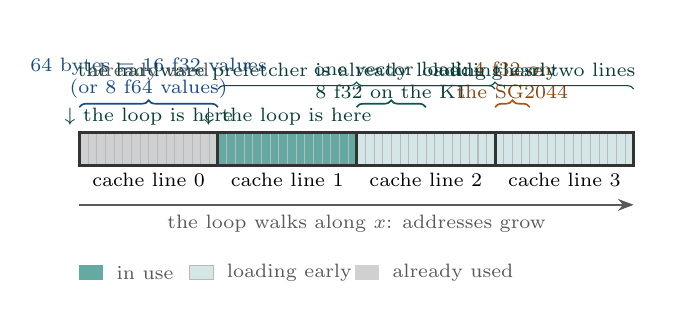
\begin{tikzpicture}[x=1cm,y=1cm]
  \tikzset{v/.style={draw=psgray!45,line width=0.2pt,fill=white},
           now/.style={fill=psteal!65}, next/.style={fill=psteal!18}, done/.style={fill=psgray!30},
           lbx/.style={font=\scriptsize,inner sep=1pt},
           vl/.style={decorate,decoration={brace,amplitude=2.5pt},line width=0.6pt}}
  \path (-0.2,-1.6) rectangle (7.5,1.75);   % the same size on every overlay
  \def\w{0.11}   % one f32 value
  \def\h{0.42}
  %   \lstate{line}{style}: colour one whole cache line
  \def\lstate#1#2#3{\fill[#2,visible on=<#3>] ({#1*16*\w},0) rectangle ++({16*\w},\h);}
  \lstate{0}{now}{2} \lstate{1}{next}{2} \lstate{2}{next}{2}
  \lstate{0}{done}{3} \lstate{1}{now}{3} \lstate{2}{next}{3} \lstate{3}{next}{3}
  \foreach \k in {0,...,63} \draw[v,fill=none] (\k*\w,0) rectangle ++(\w,\h);
  %   the cache lines: thick borders every 16 values
  \foreach \l in {0,...,3} {
    \draw[black!80,line width=1.1pt] ({\l*16*\w},0) rectangle ++({16*\w},\h);
    \node[lbx,anchor=north] at ({(\l+0.5)*16*\w},-0.05) {cache line \l};
  }
  \draw[arr] (0,-0.5) -- (64*\w,-0.5) node[pos=0.5,below,lbl] {the loop walks along $x$: addresses grow};
  %   1: what fits in one line, and one vector load
  \begin{scope}[visible on=<1>]
    \draw[vl,psblue!80!black] (0,\h+0.32) -- (16*\w,\h+0.32)
      node[midway,above=2pt,lbx,text=psblue!80!black,align=center] {64 bytes = 16 f32 values\\(or 8 f64 values)};
    \draw[vl,psteal!70!black] (32*\w,\h+0.32) -- (40*\w,\h+0.32)
      node[midway,above=2pt,lbx,text=psteal!50!black,align=center] {one vector load:\\8 f32 on the K1};
    \draw[vl,psorange!85!black] (48*\w,\h+0.32) -- (52*\w,\h+0.32)
      node[midway,above=2pt,lbx,text=psorange!70!black,align=center] {4 f32 on\\the SG2044};
  \end{scope}
  %   2, 3: the loop and the hardware prefetcher
  \foreach \o/\l in {2/0,3/1}
    \node[font=\scriptsize,text=psteal!50!black,anchor=south,inner sep=1pt,visible on=<\o>]
      at ({(\l+0.5)*16*\w},\h+0.05) {$\downarrow$ the loop is here};
  \node[lbx,anchor=south,visible on=<2>,text=psteal!50!black] at ({2*16*\w},\h+0.62)
    {the hardware prefetcher is already loading these two lines};
  \draw[decorate,decoration={brace,amplitude=2.5pt},psteal!60!black,visible on=<2>] (16*\w,\h+0.55) -- (48*\w,\h+0.55);
  \node[lbx,anchor=south,visible on=<3>,text=psteal!50!black] at ({3*16*\w},\h+0.62)
    {loading early};
  \draw[decorate,decoration={brace,amplitude=2.5pt},psteal!60!black,visible on=<3>] (32*\w,\h+0.55) -- (64*\w,\h+0.55);
  \node[lbx,anchor=south,visible on=<3>,text=psgray!90!black] at ({0.5*16*\w},\h+0.62) {already used};
  %   legend
  \begin{scope}[shift={(0,-1.45)},visible on=<2->]
    \fill[now] (0,0) rectangle ++(0.3,0.18); \node[lbl,anchor=west] at (0.35,0.09) {in use};
    \fill[next] (1.4,0) rectangle ++(0.3,0.18); \draw[psgray!45] (1.4,0) rectangle ++(0.3,0.18);
    \node[lbl,anchor=west] at (1.75,0.09) {loading early};
    \fill[done] (3.5,0) rectangle ++(0.3,0.18); \node[lbl,anchor=west] at (3.85,0.09) {already used};
  \end{scope}
\end{tikzpicture}%


    \vspace{0.5mm}
    {\footnotesize\renewcommand{\arraystretch}{1.1}
    \begin{tabular}{@{}lrr@{}}
      \toprule
      & \textbf{K1} & \textbf{SG2044}\\
      \midrule
      cache line & 64 bytes & 64 bytes\\
      values in one line, f32 / f64 & 16 / 8 & 16 / 8\\
      f32 values in one vector load & 8 & 4\\
      \bottomrule
    \end{tabular}\par}
    \todo{SG2044: 64 B from the SG2042 device tree; confirm on monte3.}
    \column{0.42\textwidth}
    \vspace{1mm}
    \begin{itemize}\small
      \item The memory does not send single numbers to the cache. It sends whole \term{cache lines} of 64 bytes.
      \item The loop walks along $x$, so it uses one cache line after the other.
      \item<2-> A \term{stream} is such a run of consecutive cache lines that the loop walks through in order.
      \item<2-> The \term{hardware prefetcher} notices a stream and loads the next lines before the loop needs
            them.
    \end{itemize}
  \end{columns}
  \takeaway{Walking through one array along $x$ is one stream: one cache line after the other.}
\end{frame}

% -----------------------------------------------------------------------------
\begin{frame}{Which accesses belong to the same stream}
  \begin{columns}[T,onlytextwidth]
    \column{0.6\textwidth}
    \vspace{1mm}
    % Slide "How many streams the stencil needs" (new in presentation5, after the user asked how many streams the
% flat arrays of the layout slide stand for). Same strip, numbers and colours as figures/fzyx.tex: the
% 3 x 3 x 3 cube stored x fastest, then y, then z; cell 13 in the middle (blue), its 6 face neighbours (teal).
% Top: if ONE array held all 7 values, the reads at 12, 13, 14 (same row, same cache line) form one stream,
% and 10 (row y-1), 16 (row y+1), 4 (plane z-1), 22 (plane z+1) one each: 5 streams (the classic 7-point
% stencil: 5 read streams + 1 written = 6, the old bullet of the stream slide).
% Bottom: our kernel (waLBerla fzyx, pull, lbmpy order): every value has its own array and is read at one place
% only, x - c_i: f_0 at 13, f_1 (N, c = (0,1,0)) at 13 - 3 = 10, f_2 (S) at 16, f_3 (W, c = (-1,0,0)) at 14,
% f_4 (E) at 12, f_5 (T, c = (0,0,1)) at 13 - 9 = 4, f_6 (B) at 22 (checked against the generated StreamCollide,
% see figures/stencil-d3q19.tex). So one stream per array: 19 read, plus 19 written (AB pattern) and 4 outputs
% (rho, u_x, u_y, u_z) = 42 (the generated loop has 19 prefetch_read + 23 prefetch_write, one per array).
% In place (AA): reads and writes use the same 19 arrays at the same addresses: 19 + 4 = 23.
% Overlays: 1 one array, 5 streams; 2 our kernel, 7 arrays, 7 streams; 3 all 19 arrays and the total.
% presentation7-v2 (user's review: "missing the important thing: the cache line and where it falls"): redrawn
% with real distances instead of the 3 x 3 x 3 toy array. Each piece is ONE cache line of 64 B = 16 f32 values
% (cache-line.tex). Real f32 strides of our arrays (fzyx.tex): row 68 values = 272 B, plane 4488 values =
% 17 952 B (about 18 KB), array 296 208 values = 1 184 832 B (about 1.2 MB). The cell x is drawn at position 6 of
% its line, so x-1 and x+1 lie in the same line (at a line border one of them falls into the next line, which the
% loop needs next anyway).
% Overlays: 1 one array holding all 7 values: 5 streams; 2 our kernel: 7 arrays, 7 streams, + 12 more = 19.
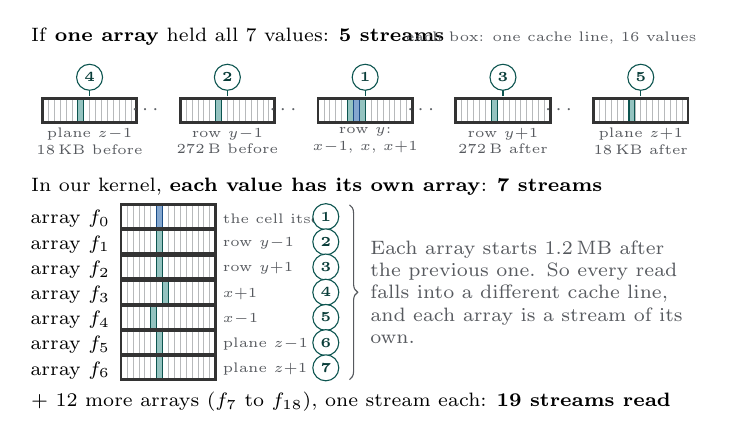
\begin{tikzpicture}[x=1cm,y=1cm]
  \tikzset{
    vv/.style={draw=psgray!45,line width=0.2pt},
    cline/.style={draw=black!80,line width=1.0pt},
    me/.style={draw=psblue!80!black,fill=psblue!55,line width=0.4pt},
    nb/.style={draw=psteal!70!black,fill=psteal!45,line width=0.4pt},
    hd/.style={font=\scriptsize,anchor=south west,inner sep=0pt},
    tl/.style={font=\tiny,text=psgray!90!black,inner sep=1pt,align=center},
    sn/.style={circle,draw=psteal!70!black,fill=white,font=\tiny\bfseries,text=psteal!50!black,
               inner sep=0.4pt,minimum size=3.3mm},
    arrlbl/.style={font=\scriptsize,anchor=east,inner sep=1pt},
  }
  \path (0,-0.3) rectangle (8.5,4.55);   % the same size on every overlay
  \def\w{0.075}\def\h{0.3}
  %   \piece{x}{y}{cells to mark: list of pos/style}: one cache line of 16 values
  \def\piece#1#2#3{%
    \foreach \k in {0,...,15} \draw[vv] (#1+\k*\w,#2) rectangle ++(\w,\h);
    \foreach \p/\st in #3 \draw[\st] (#1+\p*\w,#2) rectangle ++(\w,\h);
    \draw[cline] (#1,#2) rectangle ++(16*\w,\h);}

  % ================= 1: one array holding all 7 values ===============================================
  \node[hd] at (0,4.32) {If \textbf{one array} held all 7 values: \textbf{5 streams}};
  \foreach \i/\px/\marks/\t/\n in {
      0/0.15/{6/nb}/{plane $z{-}1$\\18\,KB before}/4,
      1/1.9/{6/nb}/{row $y{-}1$\\272\,B before}/2,
      2/3.65/{5/nb,7/nb,6/me}/{row $y$:\\$x{-}1$, $x$, $x{+}1$}/1,
      3/5.4/{6/nb}/{row $y{+}1$\\272\,B after}/3,
      4/7.15/{6/nb}/{plane $z{+}1$\\18\,KB after}/5} {
    \piece{\px}{3.35}{\marks}
    \node[tl,anchor=north] at (\px+8*\w,3.32) {\t};
    \node[sn] at (\px+8*\w,3.92) {\n};
    \draw[psteal!70!black,line width=0.4pt] (\px+8*\w,3.68) -- (\px+8*\w,3.76);
  }
  \foreach \gx in {1.35,3.1,4.85,6.6}
    \node[font=\scriptsize,text=psgray] at (\gx+0.13,3.5) {$\cdots$};
  \node[tl,anchor=south east] at (8.5,4.3) {each box: one cache line, 16 values};

  % ================= 2: our kernel, every value in its own array =====================================
  \begin{scope}[visible on=<2->]
    \node[hd] at (0,2.42) {In our kernel, \textbf{each value has its own array}: \textbf{7 streams}};
    \foreach \a/\marks/\t/\yy in {0/{6/me}/{the cell itself}/2.0, 1/{6/nb}/{row $y{-}1$}/1.68,
        2/{6/nb}/{row $y{+}1$}/1.36, 3/{7/nb}/{$x{+}1$}/1.04, 4/{5/nb}/{$x{-}1$}/0.72,
        5/{6/nb}/{plane $z{-}1$}/0.4, 6/{6/nb}/{plane $z{+}1$}/0.08} {
      \node[arrlbl] at (1.05,\yy+0.12) {array $f_{\a}$};
      \piece{1.15}{\yy}{\marks}
      \node[tl,anchor=west] at (2.4,\yy+0.13) {\t};
      \pgfmathtruncatemacro\n{\a+1}
      \node[sn] at (3.75,\yy+0.15) {\n};
    }
    \draw[decorate,decoration={brace,amplitude=3pt},psgray!90!black] (4.05,2.3) -- (4.05,0.08)
      node[midway,right=4pt,font=\scriptsize,align=left,text width=4.1cm]
      {Each array starts 1.2\,MB after the previous one. So every read falls into a different cache line,
       and each array is a stream of its own.};
  \end{scope}
  \node[font=\scriptsize,anchor=west,inner sep=0pt,visible on=<2->] at (0,-0.2)
    {+ 12 more arrays ($f_7$ to $f_{18}$), one stream each: \textbf{19 streams read}};
\end{tikzpicture}%

    \column{0.38\textwidth}
    \vspace{1mm}
    \begin{itemize}\small
      \item If one array held all values, $x-1$, $x$ and $x+1$ would lie in the same cache line: one stream.
      \item The rows $y\pm1$ (272 bytes away) and the planes $z\pm1$ (18\,KB away) lie in other lines. Each of
            them is a stream of its own: 5 in total.
      \item<2-> In our kernel, each value has its own array, 1.2\,MB after the previous one. So each of the 19
            reads is a stream of its own.
    \end{itemize}
  \end{columns}
  \takeaway{Two accesses belong to the same stream only if they fall into the same or the next cache line.
    Our loop reads 19 streams.}
\end{frame}

% -----------------------------------------------------------------------------
\begin{frame}{Our loop walks through 42 arrays at once}
  \begin{columns}[T,onlytextwidth]
    \column{0.52\textwidth}
    \vspace{1mm}
    \centering% Slide "What a data stream is": the memory one step of the inner loop touches (AB pattern, the
% generated StreamCollide kernel). Each of the 19 values of a cell has its own array (waLBerla's
% fzyx layout); pull streaming reads value i at the neighbour x - c_i (still consecutive addresses
% along x), the AB pattern writes a second set of 19 arrays, and the kernel writes rho and u
% (4 arrays): 19 + 19 + 4 = 42 sequences of consecutive addresses, all advancing together.
% Evidence: the generated StreamCollide of SweepgenLdcCPU_explicit_cse_pf (GCC f32, board) has
% exactly 19 prefetch_read and 23 prefetch_write calls in its loop, one per array it walks through.
% presentation7-v2: no overlays any more (the single-array animation moved to figures/cache-line.tex). Every box
% is one cache line of 64 bytes; all 42 arrays are at the same place of the loop (line 5).
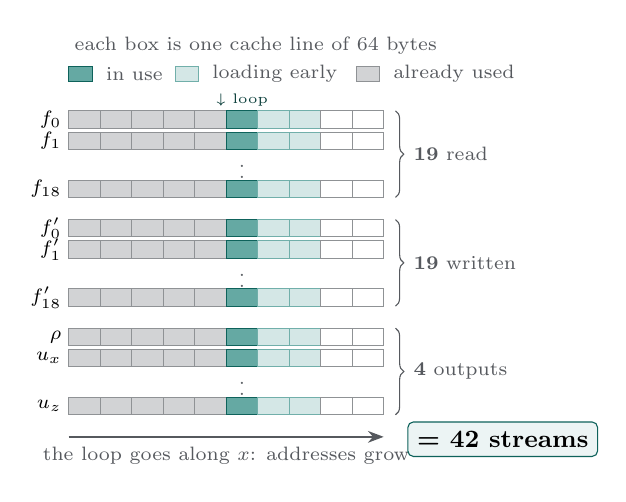
\begin{tikzpicture}[x=1cm,y=1cm]
  \tikzset{cl/.style={draw=psgray!70,fill=white,line width=0.3pt},
           clnow/.style={draw=psteal!80!black,fill=psteal!65,line width=0.3pt},
           clnext/.style={draw=psteal!60,fill=psteal!18,line width=0.3pt},
           cldone/.style={draw=psgray!70,fill=psgray!28,line width=0.3pt},
           arrlbl/.style={font=\scriptsize,anchor=east,inner sep=1pt}}
  %   \strip{y}{label}: one array as 10 cache lines; the loop is in line 5, the two after it are on their way
  \newcommand{\strip}[2]{%
    \foreach \k in {0,...,9} {
      \ifnum\k<5 \def\st{cldone}\else\ifnum\k=5 \def\st{clnow}\else
        \ifnum\k<8 \def\st{clnext}\else \def\st{cl}\fi\fi\fi
      \draw[\st] (\k*0.4,#1) rectangle ++(0.4,0.22);
    }
    \node[arrlbl] at (-0.05,#1+0.11) {#2};}
  \newcommand{\vdotsat}[1]{\node[font=\scriptsize,text=psgray] at (2.2,#1) {$\vdots$};}
  \newcommand{\grp}[4]{% y bottom, y top, count, what
    \draw[decorate,decoration={brace,amplitude=3pt},psgray!90!black] (4.15,#2) -- (4.15,#1)
      node[midway,right=3pt,font=\scriptsize,align=left] {\textbf{#3} #4};}

  \strip{3.5}{$f_0$} \strip{3.23}{$f_1$} \vdotsat{2.98} \strip{2.62}{$f_{18}$}
  \grp{2.62}{3.72}{19}{read}
  \strip{2.12}{$f'_0$} \strip{1.85}{$f'_1$} \vdotsat{1.6} \strip{1.24}{$f'_{18}$}
  \grp{1.24}{2.34}{19}{written}
  \strip{0.74}{$\rho$} \strip{0.47}{$u_x$} \vdotsat{0.22} \strip{-0.14}{$u_z$}
  \grp{-0.14}{0.96}{4}{outputs}
  \node[font=\tiny,text=psteal!50!black,anchor=south,inner sep=1pt] at (5*0.4+0.2,3.74) {$\downarrow$ loop};

  \draw[arr] (0,-0.42) -- (4.0,-0.42) node[midway,below,lbl] {the loop goes along $x$: addresses grow};
  \node[draw=psteal!80!black,fill=psteal!8,rounded corners=2pt,font=\small\bfseries,anchor=west]
    at (4.3,-0.45) {= 42 streams};
  %   legend
  \node[lbl,anchor=west] at (-0.05,4.55) {each box is one cache line of 64 bytes};
  \draw[clnow] (0,4.1) rectangle ++(0.3,0.18);
  \node[lbl,anchor=west] at (0.35,4.19) {in use};
  \draw[clnext] (1.35,4.1) rectangle ++(0.3,0.18);
  \node[lbl,anchor=west] at (1.7,4.19) {loading early};
  \draw[cldone] (3.65,4.1) rectangle ++(0.3,0.18);
  \node[lbl,anchor=west] at (4.0,4.19) {already used};
\end{tikzpicture}

    \column{0.46\textwidth}
    \vspace{1mm}
    {\small What the rows are:\par}
    \vspace{1mm}
    \begin{itemize}\small
      \item $f_0$ to $f_{18}$: the 19 values of each cell \emph{before} the time step. The loop reads them.
      \item $f'_0$ to $f'_{18}$: the 19 new values \emph{after} the step. The loop writes them into a second set
            of 19 arrays.
      \item $\rho$: the \term{density} of the fluid in each cell. $u_x$, $u_y$, $u_z$: the three parts of its
            \term{velocity}. The loop writes these 4 outputs too.
    \end{itemize}
    \vspace{1mm}
    {\small All 42 arrays advance together, one cache line after the other. The hardware prefetcher can follow
    only a limited number of streams at once.\par}
  \end{columns}
  \takeaway{19 reads + 19 writes + 4 outputs = 42 streams at once.}
\end{frame}

% -----------------------------------------------------------------------------
\subsection{Two ways to use fewer streams}
\begin{frame}{Fewer streams, way 1: update in place (the AA pattern)}
  \vspace{1mm}
  \begin{columns}[T,onlytextwidth]
    \column{0.4\textwidth}
    {\small\bfseries The usual way (AB): read A, write B\par}
    \vspace{3mm}
    \centering% The usual "AB" scheme: two arrays, A and B. Each step reads one and writes the other, then
% they swap roles. Shown next to the AA pattern (aa-pattern.tex), which uses only array A.
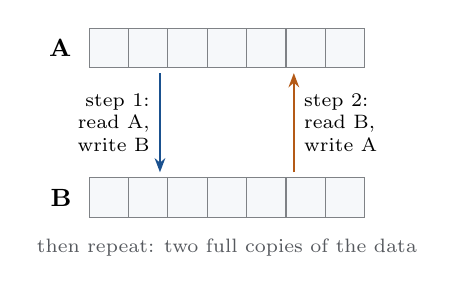
\begin{tikzpicture}[
    cell/.style={draw=psgray!80,fill=codebg,minimum width=5mm,minimum height=5mm,inner sep=0pt},
    st/.style={-{Stealth[length=1.8mm]},thick}]
  \foreach \k in {0,...,6} {
    \node[cell] at (\k*0.5+0.25,0) {};
    \node[cell] at (\k*0.5+0.25,-1.9) {};
  }
  \node[font=\small\bfseries,anchor=east] at (-0.1,0) {A};
  \node[font=\small\bfseries,anchor=east] at (-0.1,-1.9) {B};
  \draw[st,psblue!85!black] (0.9,-0.32) -- node[left,font=\scriptsize,align=right,text=black] {step 1:\\read A,\\write B} (0.9,-1.58);
  \draw[st,psorange!90!black] (2.6,-1.58) -- node[right,font=\scriptsize,align=left,text=black] {step 2:\\read B,\\write A} (2.6,-0.32);
  \node[lbl,anchor=north] at (1.75,-2.3) {then repeat: two full copies of the data};
\end{tikzpicture}


    \vspace{1mm}
    {\small\textbf{42 streams}, 260 bytes per cell\par}
    \column{0.56\textwidth}
    {\small\bfseries In place (AA): one array, two kinds of step\par}
    \vspace{1mm}
    \centering% Slide "Fewer streams, way 1: update in place (the AA pattern)": the AA pattern for one pair of directions,
% seen from cell x (as in lbmpy's AA accessors). Two of a cell's 19 slots are drawn: the slot of f_3 (the value
% moving west, D3Q19 in lbmpy's order: c_3 = (-1, 0, 0)) and the slot of f_4 (moving east, c_4 = (+1, 0, 0)).
% Even step: read both slots of x, collide, write each new value into the slot of the OPPOSITE direction of the
% same cell (so the two values swap slots and nothing moves yet). Odd step: read from the neighbours' slots (f_3
% of x-1, f_4 of x+1, where the even step left the values) and write the new values back into the same slots,
% which completes the move of both steps. Every step reads and writes the same addresses: one set of arrays.
% presentation7-v2 (user's review): the slots were labelled W and E without a definition; now f_3 and f_4 with
% arrows, and a legend that says what they are.
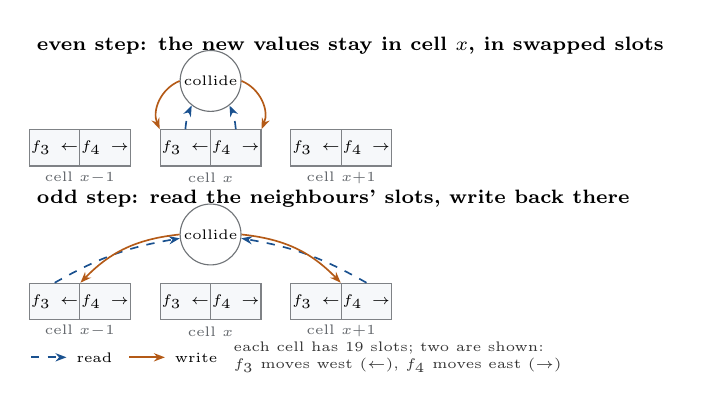
\begin{tikzpicture}[
    slot/.style={draw=psgray!80,fill=codebg,minimum width=6.4mm,minimum height=4.6mm,inner sep=0pt,font=\tiny},
    coll/.style={circle,draw=psgray!90,fill=white,inner sep=1pt,font=\tiny},
    rd/.style={-{Stealth[length=1.4mm]},semithick,draw=psblue!85!black,dashed},
    wr/.style={-{Stealth[length=1.4mm]},semithick,draw=psorange!90!black}]
  \foreach \p/\py/\ttl in {e/0/{even step: the new values stay in cell $x$, in swapped slots},
                           o/-1.95/{odd step: read the neighbours' slots, write back there}} {
    \foreach \c/\lab in {0/$x{-}1$, 1/$x$, 2/$x{+}1$} {
      \node[slot] (\p W\c) at (\c*1.66+0.3,\py) {$f_3\,\leftarrow$};
      \node[slot] (\p E\c) at (\c*1.66+0.94,\py) {$f_4\,\rightarrow$};
      \node[font=\tiny,text=psgray] at (\c*1.66+0.62,\py-0.38) {cell \lab};
    }
    \node[coll] (\p col) at (2.28,\py+0.85) {collide};
    \node[font=\scriptsize\bfseries,anchor=west] at (-0.05,\py+1.3) {\ttl};
  }
  %   even step: read both slots of x, write each new value into the other slot
  \draw[rd] (eE1.north) to[bend right=10] (ecol);
  \draw[rd] (eW1.north) to[bend left=10] (ecol);
  \draw[wr] (ecol.west) to[bend right=45] (eW1.north west);
  \draw[wr] (ecol.east) to[bend left=45] (eE1.north east);
  %   odd step: the value coming from x-1 (moving east) sits in the f_3 slot of x-1, where the even step put it;
  %   the one coming from x+1 (moving west) in the f_4 slot of x+1. The new values go back into the same two slots.
  \draw[rd] (oW0.north) to[bend left=10] (ocol);
  \draw[rd] (oE2.north) to[bend right=10] (ocol);
  \draw[wr] (ocol.east) to[bend left=20] (oE2.north west);
  \draw[wr] (ocol.west) to[bend right=20] (oW0.north east);
  %   legend
  \draw[rd] (0,-2.66) -- ++(0.45,0) node[right,font=\tiny,text=black] {read};
  \draw[wr] (1.25,-2.66) -- ++(0.45,0) node[right,font=\tiny,text=black] {write};
  \node[font=\tiny,text=black!80,anchor=west,align=left] at (2.45,-2.66)
    {each cell has 19 slots; two are shown:\\$f_3$ moves west ($\leftarrow$), $f_4$ moves east ($\rightarrow$)};
\end{tikzpicture}


    \vspace{1mm}
    {\small\textbf{23 streams}, 184 bytes per cell\par}
  \end{columns}
  \vfill
  {\scriptsize\color{psgray}Bytes per cell for f32, counting that the cache loads a line before it writes to it
  (\term{write-allocate}).\par}
  \takeaway{In place: half the arrays, 23 streams instead of 42, and less data per cell.}
\end{frame}

% -----------------------------------------------------------------------------
\begin{frame}{Fewer streams, way 2: the split loop}
  \vspace{4mm}
  \centering% Slide "The split loop: the same update in eight short passes".
% Source: submodules/walberla/apps/benchmarks/SweepgenLbmCPU/lbm_split.py (class SplitAA), used by
% SweepgenLdcCPU (--split=BY,GM,GP; CMakeLists.txt:63-70: f32 2,5,3, f64 1,5,3). For each block of BY
% rows of one z-plane the generated driver LBM_SPLIT::streamCollide calls 8 passes (generated
% SweepgenLdcCPU.cpp of explicit_cse_aa_split, e.g. build/presentation4-x86/gcc-f32/.../gen/
% SweepgenLdcCPU.cpp:6933-6997): m0..m3 add up mass and momentum of 5, 5, 5, 4 values into the scratch
% acc; macro computes rho, u (into the scratch scr, and into the outputs); c0..c2 reload 7, 6, 6
% values (the rest value and 3 opposite pairs, then 3 pairs, 3 pairs), collide (relax) them and store them in
% place. Arrays per pass: 5 / 4 outputs / 7 or 6 (plus the scratch, which stays in L1).
% Block size, 64^3 block: f32 19 x 2 rows x 64 cells x 4 B = 9728 B; f64 19 x 1 x 64 x 8 B = 9728 B.
% Scratch (driver): 9 x sc values, sc = 128 (f32) / 64 (f64): 4608 B. L1 data cache 32 KB.
% The one-loop row: the in-place (AA) StreamCollide kernel: 19 + 4 = 23 arrays (see stream-def).
% presentation7-v2 (user's review: "useless, does not convey what the split loop is for LBM; maybe a small code
% snippet"): redrawn as two short pseudo-code boxes, the one loop and the split loop, with the arrays each loop or
% pass walks through. Pass contents as in the generated driver above (m0..m3: 5, 5, 5, 4 values; macro; c0..c2: 7,
% 6, 6 values). acc: the scratch with the running sums of mass and momentum (rho, j_x, j_y, j_z per cell).
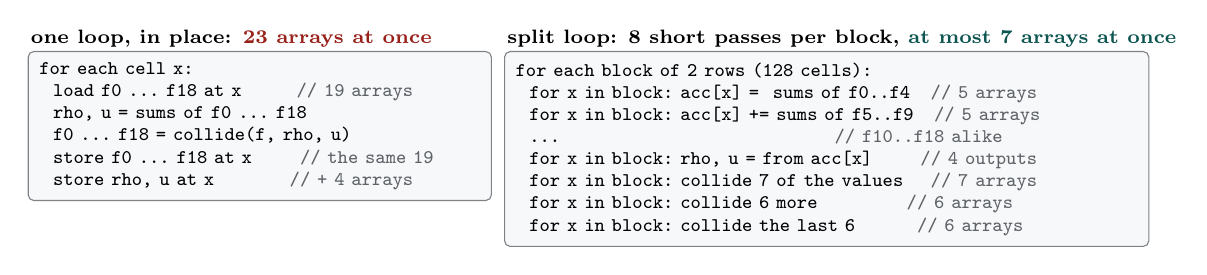
\begin{tikzpicture}
  \tikzset{cb/.style={codebox,text width=#1,font=\ttfamily\scriptsize},
           hd/.style={font=\scriptsize\bfseries,anchor=south west,inner sep=1pt}}
  \def\c#1{\textcolor{psgray}{#1}}
  \node[cb=56mm,anchor=north west] (one) at (0,0) {%
for\ each\ cell\ x:\\
\ \ load\ f0\ ...\ f18\ at\ x\ \ \ \ \ \ \ \ \c{//\ 19\ arrays}\\
\ \ rho,\ u\ =\ sums\ of\ f0\ ...\ f18\\
\ \ f0\ ...\ f18\ =\ collide(f,\ rho,\ u)\\
\ \ store\ f0\ ...\ f18\ at\ x\ \ \ \ \ \ \ \c{//\ the\ same\ 19}\\
\ \ store\ rho,\ u\ at\ x\ \ \ \ \ \ \ \ \ \ \ \c{//\ +\ 4\ arrays}};
  \node[hd] at (one.north west) {one loop, in place: \textcolor{psred!85!black}{23 arrays at once}};
  \node[cb=79mm,anchor=north west] (split) at (6.05,0) {%
for\ each\ block\ of\ 2\ rows\ (128\ cells):\\
\ \ for\ x\ in\ block:\ acc[x]\ =\ \ sums\ of\ f0..f4\ \ \ \c{//\ 5\ arrays}\\
\ \ for\ x\ in\ block:\ acc[x]\ +=\ sums\ of\ f5..f9\ \ \ \c{//\ 5\ arrays}\\
\ \ ...\ \ \ \ \ \ \ \ \ \ \ \ \ \ \ \ \ \ \ \ \ \ \ \ \ \ \ \ \ \ \ \ \ \ \ \ \ \ \ \ \c{//\ f10..f18\ alike}\\
\ \ for\ x\ in\ block:\ rho,\ u\ =\ from\ acc[x]\ \ \ \ \ \ \ \c{//\ 4\ outputs}\\
\ \ for\ x\ in\ block:\ collide\ 7\ of\ the\ values\ \ \ \ \c{//\ 7\ arrays}\\
\ \ for\ x\ in\ block:\ collide\ 6\ more\ \ \ \ \ \ \ \ \ \ \ \ \ \c{//\ 6\ arrays}\\
\ \ for\ x\ in\ block:\ collide\ the\ last\ 6\ \ \ \ \ \ \ \ \ \c{//\ 6\ arrays}};
  \node[hd] at (split.north west) {split loop: 8 short passes per block, \textcolor{psteal!70!black}{at most 7 arrays at once}};
\end{tikzpicture}%


  \vspace{2mm}
  \raggedright
  \begin{itemize}\small
    \item Collide needs $\rho$ and $u$, and they depend on all 19 values. So the split loop first adds up the values
          in four passes of at most 5 arrays, and keeps the sums in a small scratch array (\code{acc}).
    \item A block of 2 rows is small enough to stay in the L1 cache. So the three collide passes reload their
          values from L1, not from memory.
  \end{itemize}
  \vspace{1mm}
  {\scriptsize\color{psgray}One block: 19 values $\times$ 128 cells $\times$ 4 bytes = 9.7\,KB, plus 4.6\,KB of
  scratch. L1 data cache: 32\,KB per core on the K1, 64\,KB on the SG2044. f64: blocks of 1 row, the same size in
  bytes.\par}
  \takeaway{Each short pass uses at most 7 arrays, so the hardware prefetcher can follow it. The split loop always
    updates in place.}
\end{frame}

% =============================================================================
\section[Part 1: K1]{Part 1: SpacemiT K1 (256-bit vectors)}
\subsection{The hardware and its limit}

\begin{frame}{K1: the hardware}
  \vspace{3mm}
  \centering% Slide "The hardware, and how the work is split": the SpacemiT K1 on the Banana Pi BPI-F3
% (report r03, table "test system"): 8 X60 cores at 1.6 GHz in two clusters of 4; L1D 32 KiB per
% core, L2 512 KiB per cluster, no L3; 4 GB memory, about 357 cycles per DRAM miss (pointer chase,
% huge pages). The benchmark runs one MPI process with one 64^3 block per core.
% Cache line 64 B: read on the board (sysfs coherency_line_size of L1I, L1D, L2; device tree), 2026-11-23.
% Right: one X60 core's 256-bit vector register as 8 f32 or 4 f64 lanes.
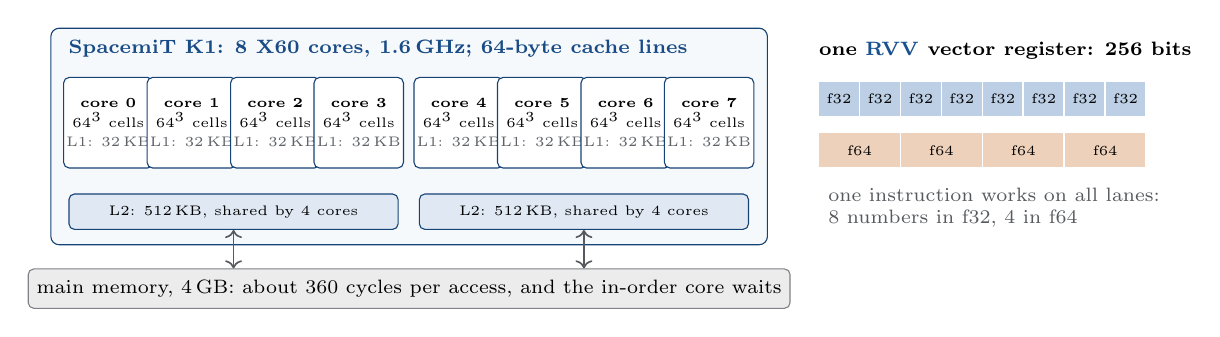
\begin{tikzpicture}[
    core/.style={box,minimum width=0.98cm,minimum height=1.15cm,fill=white,draw=psblue!70!black,
      font=\tiny,align=center,inner sep=1pt},
    l2/.style={box,fill=psblue!14,draw=psblue!70!black,font=\tiny,minimum height=4.5mm,inner sep=1pt},
    ln/.style={draw=white,line width=0.6pt,minimum height=4.5mm,inner sep=0pt,font=\tiny}]
  % ---- the chip -------------------------------------------------------------------
  \draw[psblue!70!black,fill=psblue!4,rounded corners=3pt] (0,0) rectangle (9.1,2.75);
  \node[anchor=north west,font=\scriptsize\bfseries,text=psblue!80!black] at (0.1,2.72)
    {SpacemiT K1: 8 X60 cores, 1.6\,GHz; 64-byte cache lines};
  \foreach \c/\xo in {0/0.2,1/4.65} {
    \foreach \k in {0,...,3} {
      \pgfmathtruncatemacro{\n}{4*\c+\k}
      \node[core] at (\xo+0.53+\k*1.06,1.55) {\textbf{core \n}\\[1pt]$64^3$ cells\\[1pt]{\color{psgray}L1: 32\,KB}};
    }
    \node[l2,minimum width=4.18cm] (l\c) at (\xo+2.12,0.42) {L2: 512\,KB, shared by 4 cores};
  }
  % ---- main memory -------------------------------------------------------------------
  \node[box,fill=psgray!12,minimum width=9.1cm,minimum height=5mm,font=\scriptsize,anchor=north]
    (mem) at (4.55,-0.3) {main memory, 4\,GB: about 360 cycles per access, and the in-order core waits};
  \foreach \c in {0,1} \draw[<->,semithick,psgray!90!black] (l\c.south) -- (l\c.south |- mem.north);

  % ---- one core's vector register --------------------------------------------------
  \begin{scope}[shift={(9.75,0.25)}]
    \def\w{0.52}
    \node[font=\scriptsize\bfseries,anchor=south west,inner sep=0pt] at (0,2.1) {one \term{RVV} vector register: 256 bits};
    \foreach \k in {0,...,7}
      \node[ln,fill=psblue!30,minimum width=\w cm] at (\k*\w+\w/2,1.6) {f32};
    \foreach \k in {0,...,3}
      \node[ln,fill=psorange!30,minimum width=2*\w cm] at (\k*2*\w+\w,0.95) {f64};
    \node[lbl,anchor=north west,align=left] at (0,0.6)
      {one instruction works on all lanes:\\8 numbers in f32, 4 in f64};
  \end{scope}
\end{tikzpicture}


  \vspace{4mm}
  \raggedright
  \begin{itemize}\small
    \item Banana Pi BPI-F3 board with 8 SpacemiT X60 cores.
    \item The X60 runs instructions \term{in order}: when a load misses the cache, the core waits.
    \item The X60 executes the RISC-V prefetch instructions (\term{Zicbop}), although its list of extensions does
          not name them. We measured this (later in this part).
  \end{itemize}
  \takeaway{K1: 256-bit vectors, 8 cores, 4\,GB memory, no L3 cache.}
\end{frame}

% -----------------------------------------------------------------------------
%  Plot and numbers unchanged from presentation6 (figures/streams.tex has the sources: presentation4
%  streams_check.sh, streams-probe.log, streams-ldc.log; notes5 F3, F7, F19, F20).
\begin{frame}{K1: the limit is the number of streams}
  \begin{columns}[T,onlytextwidth]
    \column{0.52\textwidth}
    \centering% Slide "The real limit: too many data streams": the stream test of report 3 (misc/x60-lab/probes/mem.cpp,
% unchanged; code on the next slide) rerun for presentation4 with the X60's own counters:
% scripts/presentation4/streams_check.sh, log docs/presentation4/board-logs/board/streams-probe.log,
% coordinates printed by
%   python3 scripts/presentation4/streams_table.py --tex docs/presentation4/board-logs/board
% R read streams of 4 MB each (f32 vector loads, huge pages requested), one X60 core (core 2).
% Top: cycles per 64-byte line (the probe's own cycle counter, runs without perf's cycles event).
% Bottom ("late lines"): l2_miss per line = lines that missed L2 on access, i.e. were not prefetched in time (every
% line comes from DRAM: 4 MB per array, L2 512 KB), (count(3 passes) - count(0 passes)) / lines.
% Three array offsets (stagger 4160, 1600, 12352 bytes): the cliff stays at 20 to 22 streams; the addresses
% still change the cost below it (1600 B: up to 1.7x the cycles, 0.206 late per line at R = 10; notes5 F20). Tag d (4160 again, at the end) repeats tag a:
% e.g. R = 8: 19.2 / 19.2, R = 24: 364.7 / 364.6 cycles. With software prefetch (prefetch.r 512 B
% ahead, tag c) R = 20 ... 23 cost 96 to 102 cycles instead of 110 to 361, but R = 14 ... 19 cost 2 to 3.6x more
% than without (notes5 F7); that series has no counter run, so it is only in the top panel. Every series is
% one run, except 4160 B (tags a and d). presentation5: log-axis and late-share labels, legend note (notes5 F20).
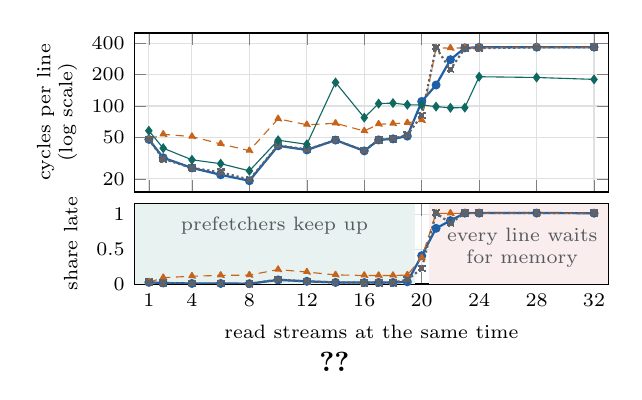
\begin{tikzpicture}
  \pgfplotsset{st/.style={width=7.6cm, ylabel style={at={(axis description cs:-0.1,0.5)}}, xmin=0, xmax=33, xtick={1,4,8,12,16,20,24,28,32},
      tick label style={font=\scriptsize}, label style={font=\scriptsize},
      grid=major, grid style={psgray!20}},
    sa/.style={color=psblue,mark=*,mark size=1.2pt,thick},
    sb1/.style={color=psorange,mark=triangle*,mark size=1.4pt,densely dashed},
    sb2/.style={color=psgray,mark=square*,mark size=1.0pt,densely dotted,thick},
    sc/.style={color=psteal!85!black,mark=diamond*,mark size=1.5pt}}
  \begin{semilogyaxis}[st, name=top, height=3.6cm, ymin=15, ymax=500,
      ytick={20,50,100,200,400}, yticklabels={20,50,100,200,400}, xticklabels={},
      ylabel={cycles per line\\(log scale)}, ylabel style={align=center},
      legend to name=streamsleg, legend columns=2, legend cell align=left,
      legend style={font=\tiny,draw=psgray!50,inner sep=1pt,/tikz/every even column/.append style={column sep=4pt}}]
    \addplot[sa] coordinates {(1,47.8) (2,31.9) (4,25.5) (6,21.9) (8,19.2) (10,41.5) (12,37.9) (14,47.1)
      (16,37.1) (17,47.3) (18,48.4) (19,51.4) (20,110.5) (21,158.8) (22,277.8) (23,360.6) (24,364.7)
      (28,365.9) (32,366.1)};
    \addplot[sb1] coordinates {(1,47.9) (2,53.5) (4,50.9) (6,43.3) (8,37.3) (10,75.3) (12,66.1) (14,68.2)
      (16,57.6) (17,66.9) (18,67.7) (19,68.9) (20,72.9) (21,360.2) (22,358.5) (23,360.0) (24,361.9)
      (28,364.5) (32,363.9)};
    \addplot[sb2] coordinates {(1,47.8) (2,31.1) (4,25.5) (6,23.2) (8,19.7) (10,42.0) (12,38.3) (14,47.0)
      (16,37.4) (17,47.4) (18,48.6) (19,52.8) (20,80.9) (21,362.0) (22,224.0) (23,356.7) (24,358.0)
      (28,364.2) (32,366.1)};
    \addplot[sc] coordinates {(1,57.9) (2,39.4) (4,30.5) (6,28.0) (8,23.9) (10,47.0) (12,42.9) (14,168.0)
      (16,77.3) (17,105.3) (18,106.6) (19,102.7) (20,102.2) (21,98.6) (22,96.1) (23,96.4) (24,190.7)
      (28,187.5) (32,179.8)};
    \legend{arrays 4160 B apart, 1600 B apart, 12352 B apart, 4160 B + software prefetch (top only)}
  \end{semilogyaxis}
  \begin{axis}[st, name=bottom, at={(top.south)}, anchor=north, yshift=-1.5mm, height=2.6cm, ymin=0, ymax=1.15,
      ytick={0,0.5,1}, ylabel={share late}, xlabel={read streams at the same time}]
    \fill[psteal!10] (axis cs:0,0) rectangle (axis cs:19.5,1.15);
    \fill[psred!8] (axis cs:20.5,0) rectangle (axis cs:33,1.15);
    \node[lbl,anchor=north] at (axis cs:9.75,1.1) {prefetchers keep up};
    \node[lbl,anchor=south] at (axis cs:27,0.1) {every line waits\\for memory};
    \addplot[sa] coordinates {(1,0.023) (2,0.014) (4,0.007) (6,0.007) (8,0.004) (10,0.058) (12,0.038)
      (14,0.022) (16,0.020) (17,0.022) (18,0.021) (19,0.031) (20,0.406) (21,0.798) (22,0.909) (23,1.016)
      (24,1.016) (28,1.017) (32,1.015)};
    \addplot[sb1] coordinates {(1,0.024) (2,0.090) (4,0.111) (6,0.123) (8,0.127) (10,0.206) (12,0.171)
      (14,0.130) (16,0.122) (17,0.121) (18,0.121) (19,0.128) (20,0.376) (21,1.013) (22,1.013) (23,1.012)
      (24,1.012) (28,1.012) (32,1.013)};
    \addplot[sb2] coordinates {(1,0.023) (2,0.014) (4,0.005) (6,0.005) (8,0.003) (10,0.064) (12,0.037)
      (14,0.021) (16,0.019) (17,0.018) (18,0.019) (19,0.061) (20,0.221) (21,1.017) (22,0.870) (23,1.017)
      (24,1.020) (28,1.016) (32,1.016)};
  \end{axis}
  \node[anchor=north,inner sep=0pt] at ([yshift=-0.5mm]bottom.outer south) {\ref{streamsleg}};
\end{tikzpicture}

    \column{0.46\textwidth}
    \vspace{1mm}
    \machine{K1}
    \begin{itemize}\small
      \item Up to 19 streams, the hardware prefetcher brings most lines in time.
      \item From about 21 streams on, every vector load waits for memory: about 360 cycles.
      \item Our loop has 42 streams.
    \end{itemize}
  \end{columns}
  \vspace{0.5mm}
  {\scriptsize\color{psgray}A test loop that reads $R$ arrays (next slide); the core's own counters; one run per
  point.\par}
  \takeaway{The K1 follows about 20 streams. With 42, the core waits in 92\,\% of its cycles.}
\end{frame}

% -----------------------------------------------------------------------------
\begin{frame}{K1: the stream test behind the plot}
  \vspace{2mm}
  \centering% Slide "The stream test: the code behind the plot".
% Top: the timed loop of misc/x60-lab/probes/mem.cpp, function stream() (lines 124-158), simplified:
% the real code adds the 8 loads with a sum tree (a0+a1, a2+a3, ...) so they do not wait for each
% other, and has further options (touch-ahead loads, prefetch.w, cbo.zero, scalar loads) not used here.
% Each array is 4 MB (f32); the time is the best of 3 passes, read with the cycle counter
% (perf_event_open, probes/pmu.hpp). Built with g++ -O2 -march=rv64gcv_zvl256b_zicboz.
% Bottom: the commands and their results, all from presentation4's runs (scripts/presentation4/streams_check.sh):
% first three docs/presentation4/board-logs/board/streams-probe.log (tags a and c, reps=3), last two
% streams-pattern.log (best of 3 runs: 180.7 / 181.9 / 176.3 and 90.0 / 91.0 / 90.8; report 3 had 184.3 and 90.4).
% Printed by streams_table.py --tex; checked by check_figures.py.
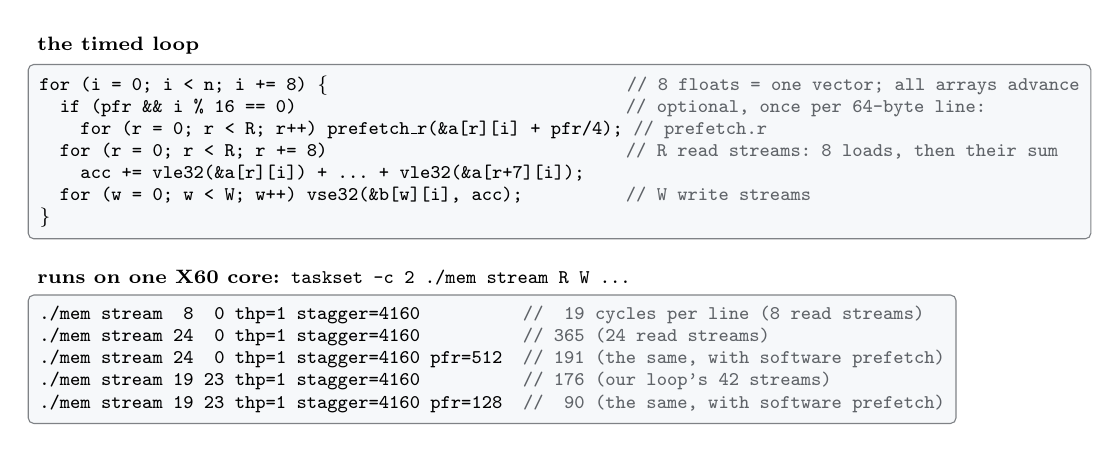
\begin{tikzpicture}
  \node[codebox,anchor=north west] (loop) at (0,0) {%
for\ (i\ =\ 0;\ i\ <\ n;\ i\ +=\ 8)\ \{\ \ \ \ \ \ \ \ \ \ \ \ \ \ \ \ \ \ \ \ \ \ \ \ \ \ \ \ \ \textcolor{psgray}{//\ 8\ floats\ =\ one\ vector;\ all\ arrays\ advance}\\
\ \ if\ (pfr\ \&\&\ i\ \%\ 16\ ==\ 0)\ \ \ \ \ \ \ \ \ \ \ \ \ \ \ \ \ \ \ \ \ \ \ \ \ \ \ \ \ \ \ \ \textcolor{psgray}{//\ optional,\ once\ per\ 64-byte\ line:}\\
\ \ \ \ for\ (r\ =\ 0;\ r\ <\ R;\ r++)\ prefetch\_r(\&a[r][i]\ +\ pfr/4);\ \textcolor{psgray}{//\ prefetch.r}\\
\ \ for\ (r\ =\ 0;\ r\ <\ R;\ r\ +=\ 8)\ \ \ \ \ \ \ \ \ \ \ \ \ \ \ \ \ \ \ \ \ \ \ \ \ \ \ \ \ \textcolor{psgray}{//\ R\ read\ streams:\ 8\ loads,\ then\ their\ sum}\\
\ \ \ \ acc\ +=\ vle32(\&a[r][i])\ +\ ...\ +\ vle32(\&a[r+7][i]);\\
\ \ for\ (w\ =\ 0;\ w\ <\ W;\ w++)\ vse32(\&b[w][i],\ acc);\ \ \ \ \ \ \ \ \ \ \textcolor{psgray}{//\ W\ write\ streams}\\
\}};
  \node[font=\scriptsize\bfseries,anchor=south west] at (loop.north west) {the timed loop};
  \node[codebox,anchor=north west] (cmd) at ([yshift=-7mm]loop.south west) {%
./mem\ stream\ \ 8\ \ 0\ thp=1\ stagger=4160\ \ \ \ \ \ \ \ \ \ \textcolor{psgray}{//\ \ 19\ cycles\ per\ line\ (8\ read\ streams)}\\
./mem\ stream\ 24\ \ 0\ thp=1\ stagger=4160\ \ \ \ \ \ \ \ \ \ \textcolor{psgray}{//\ 365\ (24\ read\ streams)}\\
./mem\ stream\ 24\ \ 0\ thp=1\ stagger=4160\ pfr=512\ \ \textcolor{psgray}{//\ 191\ (the\ same,\ with\ software\ prefetch)}\\
./mem\ stream\ 19\ 23\ thp=1\ stagger=4160\ \ \ \ \ \ \ \ \ \ \textcolor{psgray}{//\ 176\ (our\ loop's\ 42\ streams)}\\
./mem\ stream\ 19\ 23\ thp=1\ stagger=4160\ pfr=128\ \ \textcolor{psgray}{//\ \ 90\ (the\ same,\ with\ software\ prefetch)}};
  \node[font=\scriptsize\bfseries,anchor=south west] at (cmd.north west) {runs on one X60 core: \code{taskset -c 2 ./mem stream R W ...}};
\end{tikzpicture}


  \vspace{2mm}
  {\scriptsize\color{psgray}\machine{K1} Arrays of 4\,MB on \term{huge pages}, 4160 bytes apart; best of 3
  passes.\par}
  \takeaway{With 42 streams a cache line costs 176 cycles. With prefetching 128 bytes ahead it costs 90.}
\end{frame}

% -----------------------------------------------------------------------------
\subsection{Software prefetch}
%  figures/prefetch-idea.tex has the sources (prefetch distance, loop step, memory latency).
\begin{frame}{K1: what a software prefetch does}
  \vspace{1mm}
  \centering% Slide "K1: what a software prefetch does" (new in presentation7-v2; the user asked whether a prefetch also acts
% as a load and whether loads are replaced by prefetches: no, the prefetch is added, the load stays).
% Top: one array in f32, 4 cache lines of 64 B = 16 values (cache-line.tex). The vector loop step is 8 values on
% the K1 (VLEN 256); the generated prefetch distance is 128 B = 32 f32 values (--prefetch-distance=128,
% apps/benchmarks/SweepgenLdcCPU/CMakeLists.txt; prefetch-insert.tex), i.e. two lines ahead.
% Bottom: a sketch of the time line of one stream (not to scale). About 360 cycles per memory access on the K1
% (k1.tex: pointer chase, about 357 cycles); the in-order X60 waits for a load that misses. With prefetch the line
% is requested two lines (4 loop steps) earlier and is in the cache when the load comes.
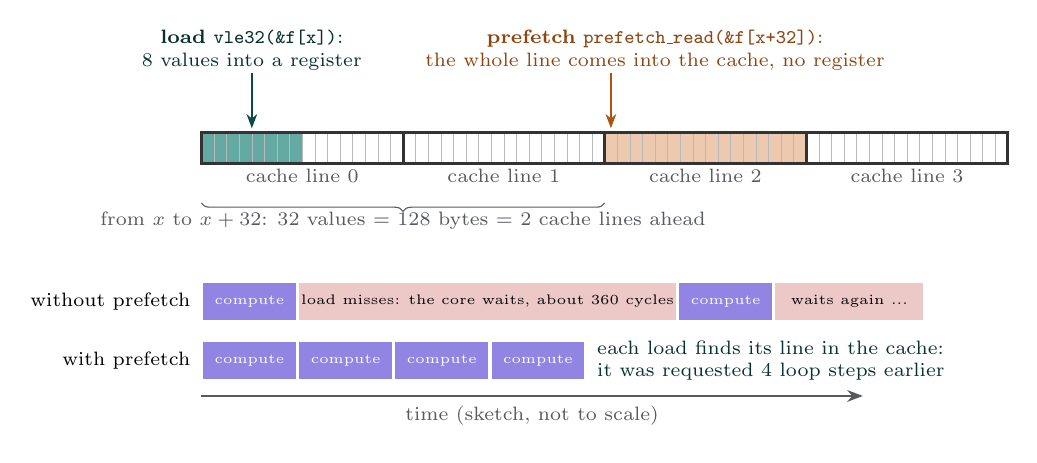
\begin{tikzpicture}[x=1cm,y=1cm]
  \tikzset{v/.style={draw=psgray!45,line width=0.2pt},
           lbx/.style={font=\scriptsize,inner sep=1pt},
           tseg/.style={draw=white,line width=0.6pt,minimum height=5mm,inner sep=1pt,font=\tiny,anchor=west}}
  \def\w{0.16}\def\h{0.4}
  % ---- the array -------------------------------------------------------------------------
  \fill[psteal!65] (0,0) rectangle (8*\w,\h);
  \fill[psorange!35] (32*\w,0) rectangle (48*\w,\h);
  \foreach \k in {0,...,63} \draw[v] (\k*\w,0) rectangle ++(\w,\h);
  \foreach \l in {0,...,3} {
    \draw[black!80,line width=1.1pt] ({\l*16*\w},0) rectangle ++({16*\w},\h);
    \node[lbx,anchor=north,text=psgray!90!black] at ({(\l+0.5)*16*\w},-0.03) {cache line \l};
  }
  \draw[-{Stealth[length=1.8mm]},thick,psteal!60!black] (4*\w,\h+0.75) -- (4*\w,\h+0.05);
  \node[lbx,anchor=south,align=center,text=psteal!40!black] at (4*\w,\h+0.75)
    {\textbf{load} \code{vle32(\&f[x])}:\\8 values into a register};
  \draw[-{Stealth[length=1.8mm]},thick,psorange!85!black] (32.5*\w,\h+0.75) -- (32.5*\w,\h+0.05);
  \node[lbx,anchor=south,align=center,text=psorange!70!black] at (36*\w,\h+0.75)
    {\textbf{prefetch} \code{prefetch\_read(\&f[x+32])}:\\the whole line comes into the cache, no register};
  \draw[decorate,decoration={brace,amplitude=3pt,mirror},psgray!90!black] (0,-0.5) -- (32*\w,-0.5)
    node[midway,below=2pt,lbx,text=psgray!90!black] {from $x$ to $x+32$: 32 values = 128 bytes = 2 cache lines ahead};

  % ---- the time line -------------------------------------------------------------------
  \begin{scope}[shift={(0,-1.75)}]
    \node[lbx,anchor=east] at (-0.1,0) {without prefetch};
    \node[tseg,fill=ckernel!70,text=white,minimum width=1.2cm] (a1) at (0,0) {compute};
    \node[tseg,fill=psred!25,minimum width=3.6cm] (a2) at (a1.east) {load misses: the core waits, about 360 cycles};
    \node[tseg,fill=ckernel!70,text=white,minimum width=1.2cm] (a3) at (a2.east) {compute};
    \node[tseg,fill=psred!25,minimum width=1.9cm] (a4) at (a3.east) {waits again ...};
    \node[lbx,anchor=east] at (-0.1,-0.75) {with prefetch};
    \node[tseg,fill=ckernel!70,text=white,minimum width=1.2cm] (b1) at (0,-0.75) {compute};
    \node[tseg,fill=ckernel!70,text=white,minimum width=1.2cm] (b2) at (b1.east) {compute};
    \node[tseg,fill=ckernel!70,text=white,minimum width=1.2cm] (b3) at (b2.east) {compute};
    \node[tseg,fill=ckernel!70,text=white,minimum width=1.2cm] (b4) at (b3.east) {compute};
    \node[lbx,anchor=west,align=left,text=psteal!40!black] at ([xshift=1mm]b4.east)
      {each load finds its line in the cache:\\it was requested 4 loop steps earlier};
    \draw[arr] (0,-1.2) -- (8.4,-1.2) node[pos=0.5,below,lbl] {time (sketch, not to scale)};
  \end{scope}
\end{tikzpicture}%


  \vspace{0mm}
  \raggedright
  {\small A \term{software prefetch} is an extra instruction. It loads nothing into a register and returns
  nothing: it only asks the cache to fetch a line early. The load stays in the code, and later finds its line
  in the cache.\par}
  \takeaway{Prefetch does not replace the loads. It brings their cache lines in before the loads need them.}
\end{frame}

% -----------------------------------------------------------------------------
\begin{frame}{K1: software prefetch in the generated code}
  \vspace{0mm}
  \centering% Slide "Software prefetch: where the code generator puts it".
% Left: where the pass sits (submodules/pystencils/src/pystencils/codegen/driver.py:313-315: after the
% vector loops are prepared, before the RVV intrinsics are chosen); the pass is
% backend/transformations/insert_prefetches.py, the option cpu.vectorize.prefetch_distance
% (codegen/config.py:278), set by the app (apps/benchmarks/SweepgenLdcCPU/CMakeLists.txt:58,
% --prefetch-distance=128; SweepgenLdcCPU.py:76-77).
% Right, top: the generated StreamCollide of SweepgenLdcCPU_explicit_cse_pf, GCC f32 (board file
% build-gcc-f32/apps/benchmarks/SweepgenLdcCPU/_gen/SweepgenLdcCPU_explicit_cse_pf/gen/SweepgenLdcCPU.cpp,
% lines 96-150), shortened: namespaces dropped, 19 + 23 calls shown as 2 + 1. Right, bottom: the
% runtime function (include/pystencils_runtime/rvv.hpp:144-151, the branch without -march=..._zicbop).
% presentation7-v2 (user's review: "not clear if prefetching also acts as a load; are we replacing load
% intrinsics with prefetch ones?"): the right side is now the same loop without and with the new pass, so that
% one sees the loads stay and the prefetches are added in front of them. The runtime function moved to the
% Zicbop slide only (zicbop.tex).
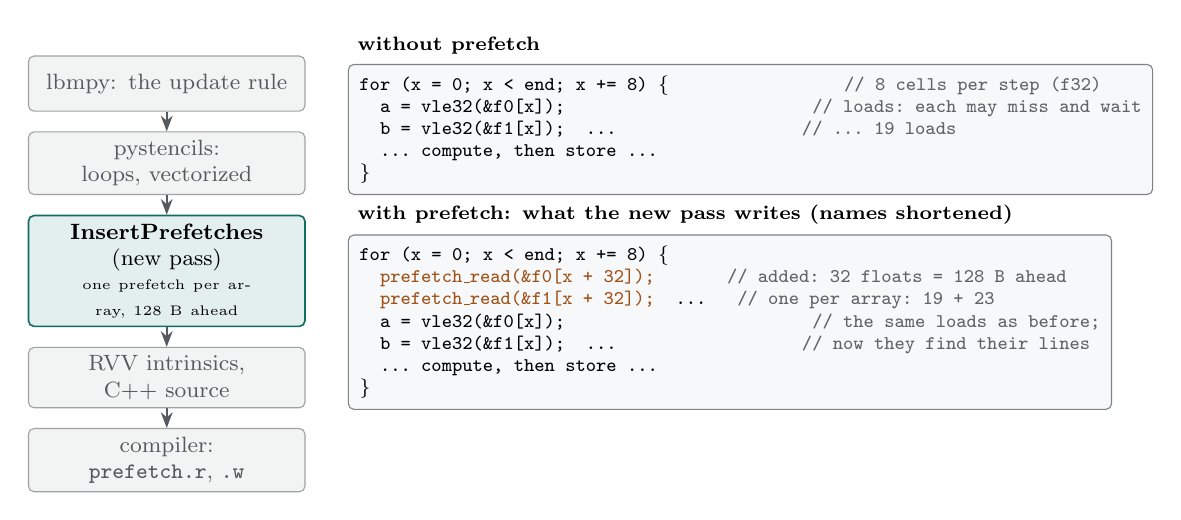
\begin{tikzpicture}
  \tikzset{st/.style={box,text width=33mm,font=\scriptsize,minimum height=5mm,inner sep=2pt}}
  \node[st,quiet] (b1) at (0,0) {lbmpy: the update rule};
  \node[st,quiet,below=2.5mm of b1] (b2) {pystencils: loops, vectorized};
  \node[st,added,below=2.5mm of b2] (b3) {\textbf{InsertPrefetches} (new pass)\\[-1pt]
    {\tiny one prefetch per array, 128 B ahead}};
  \node[st,quiet,below=2.5mm of b3] (b4) {RVV intrinsics, C++ source};
  \node[st,quiet,below=2.5mm of b4] (b5) {compiler: \code{prefetch.r}, \code{.w}};
  \foreach \a/\b in {b1/b2,b2/b3,b3/b4,b4/b5} \draw[arr] (\a) -- (\b);
  \node[codebox,anchor=north west] (old) at (2.3,0.25) {%
for\ (x\ =\ 0;\ x\ <\ end;\ x\ +=\ 8)\ \{\ \ \ \ \ \ \ \ \ \ \ \ \ \ \ \ \ \textcolor{psgray}{//\ 8\ cells\ per\ step\ (f32)}\\
\ \ a\ =\ vle32(\&f0[x]);\ \ \ \ \ \ \ \ \ \ \ \ \ \ \ \ \ \ \ \ \ \ \ \ \textcolor{psgray}{//\ loads:\ each\ may\ miss\ and\ wait}\\
\ \ b\ =\ vle32(\&f1[x]);\ \ ...\ \ \ \ \ \ \ \ \ \ \ \ \ \ \ \ \ \ \textcolor{psgray}{//\ ...\ 19\ loads}\\
\ \ ...\ compute,\ then\ store\ ...\\
\}};
  \node[font=\scriptsize\bfseries,anchor=south west] at (old.north west) {without prefetch};
  \node[codebox,anchor=north west] (new) at ([yshift=-5mm]old.south west) {%
for\ (x\ =\ 0;\ x\ <\ end;\ x\ +=\ 8)\ \{\\
\ \ \textcolor{psorange!80!black}{\textbf{prefetch\_read(\&f0[x\ +\ 32]);}}\ \ \ \ \ \ \ \textcolor{psgray}{//\ added:\ 32\ floats\ =\ 128\ B\ ahead}\\
\ \ \textcolor{psorange!80!black}{\textbf{prefetch\_read(\&f1[x\ +\ 32]);}}\ \ ...\ \ \ \textcolor{psgray}{//\ one\ per\ array:\ 19\ +\ 23}\\
\ \ a\ =\ vle32(\&f0[x]);\ \ \ \ \ \ \ \ \ \ \ \ \ \ \ \ \ \ \ \ \ \ \ \ \textcolor{psgray}{//\ the\ same\ loads\ as\ before;}\\
\ \ b\ =\ vle32(\&f1[x]);\ \ ...\ \ \ \ \ \ \ \ \ \ \ \ \ \ \ \ \ \ \textcolor{psgray}{//\ now\ they\ find\ their\ lines}\\
\ \ ...\ compute,\ then\ store\ ...\\
\}};
  \node[font=\scriptsize\bfseries,anchor=south west] at (new.north west) {with prefetch: what the new pass writes (names shortened)};
\end{tikzpicture}%


  \vspace{0mm}
  {\scriptsize\color{psgray}42 prefetches per step: 19 for the arrays the loop reads, 23 for those it writes.
  A step covers half a line, so each line is requested twice, which is cheap.\par}
  \takeaway{A new pass adds one prefetch for every array of a vector loop. The loads stay as they were.}
\end{frame}

% -----------------------------------------------------------------------------
\begin{frame}{K1: the RISC-V prefetch instruction}
  \begin{columns}[T,onlytextwidth]
    \column{0.56\textwidth}
    % Slide "Software prefetch: the RISC-V instruction behind it".
% Top: the 32-bit word of prefetch.r 0(a0) = ori x0, a0, 1 = 0x00156013. Fields (bit 31 on the left):
% imm[11:5] = offset/32 (here 0), imm[4:0] = type (0 = prefetch.i, 1 = prefetch.r, 3 = prefetch.w),
% rs1 = a0 = x10 = 01010, funct3 = 110 (ORI), rd = x0, opcode = 0010011 (OP-IMM: arithmetic with a
% constant). Checked on the laptop: riscv64-linux-gnu-g++ 16.2.1 -O3 -march=rv64gcv -c, then
% llvm-objdump -d prints "00156013  prefetch.r 0x0(a0)" for asm volatile("ori x0, %0, 1").
% Middle: the two readings of the same word. "X60 runs it": the stream test 176 -> 90 cycles per line
% with pfr=128 (board-logs/board/streams-pattern.log); notes3 progress log: the X60's ISA string lists
% zicbom and zicboz but not zicbop.
% Bottom: include/pystencils_runtime/rvv.hpp:144-151 (submodules/pystencils/src/pystencils/), shortened
% (comments added). GCC 16.2.1 with -march=rv64gcv compiles __builtin_prefetch to nothing, with
% -march=rv64gcv_zicbop to prefetch.r/prefetch.w (checked on the laptop; notes3 says the same of GCC 14).
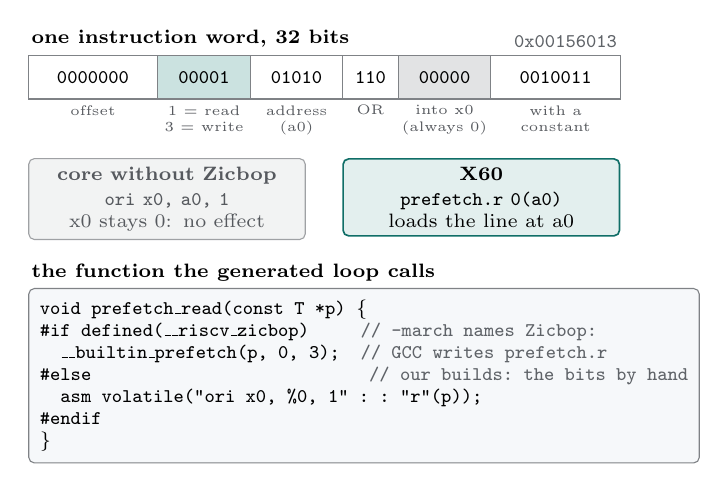
\begin{tikzpicture}
  \def\bw{2.35mm}   % width of one bit
  \def\bh{5.5mm}    % height of the word
  % field: first bit from the left (0 = bit 31) / number of bits / bits / label below / fill
  \foreach \s/\n/\bits/\lab/\fil in {
      0/7/0000000/{offset}/white,
      7/5/00001/{1 = read\\3 = write}/psteal!22,
      12/5/01010/{address\\(a0)}/white,
      17/3/110/{OR}/white,
      20/5/00000/{into x0\\(always 0)}/psgray!18,
      25/7/0010011/{with a\\constant}/white} {
    \draw[psgray!80,fill=\fil] (\s*\bw,0) rectangle ++(\n*\bw,\bh);
    \node[font=\ttfamily\scriptsize] at (\s*\bw+\n*\bw/2,\bh/2) {\bits};
    \node[lbl,anchor=north,font=\tiny,inner sep=1pt] at (\s*\bw+\n*\bw/2,-0.4mm) {\lab};
  }
  \node[font=\scriptsize\bfseries,anchor=south west,inner sep=1pt] at (0,\bh+0.6mm)
    {one instruction word, 32 bits};
  \node[font=\scriptsize,text=psgray,anchor=south east,inner sep=1pt] at (32*\bw,\bh+0.6mm)
    {\code{0x00156013}};
  % the two readings of the same bits
  \node[box,quiet,text width=33mm,font=\scriptsize,anchor=north west] (old) at (0,-7.5mm)
    {\textbf{core without Zicbop}\\[1pt]\code{ori x0, a0, 1}\\x0 stays 0: no effect};
  \node[box,added,text width=33mm,font=\scriptsize,anchor=north east] (new) at (32*\bw,-7.5mm)
    {\textbf{X60}\\[1pt]\code{prefetch.r 0(a0)}\\loads the line at a0};
  % the runtime function that the generated loop calls
  \node[codebox,anchor=north west] (rt) at (0,-24mm) {%
void\ prefetch\_read(const\ T\ *p)\ \{\\
\#if\ defined(\_\_riscv\_zicbop)\ \ \ \ \ \textcolor{psgray}{//\ -march\ names\ Zicbop:}\\
\ \ \_\_builtin\_prefetch(p,\ 0,\ 3);\ \ \textcolor{psgray}{//\ GCC\ writes\ prefetch.r}\\
\#else\ \ \ \ \ \ \ \ \ \ \ \ \ \ \ \ \ \ \ \ \ \ \ \ \ \ \ \textcolor{psgray}{//\ our\ builds:\ the\ bits\ by\ hand}\\
\ \ asm\ volatile("ori\ x0,\ \%0,\ 1"\ :\ :\ "r"(p));\\
\#endif\\
\}};
  \node[font=\scriptsize\bfseries,anchor=south west,inner sep=1pt] at ([yshift=0.4mm]rt.north west)
    {the function the generated loop calls};
\end{tikzpicture}

    \column{0.41\textwidth}
    \vspace{1mm}
    \begin{itemize}\small
      \item RVV has no prefetch. It comes from a small scalar extension, \term{Zicbop}.
      \item Its target register is x0, which is always 0. So it never produces a value and cannot replace a load.
      \item It is a \term{hint}: cores without Zicbop run it as an instruction that does nothing.
      \item The X60 runs Zicbop, but its list of extensions does not name it. So we write the instruction by hand
            (\term{inline assembly}).
    \end{itemize}
  \end{columns}
  \takeaway{Prefetch is safe on any RISC-V core. On the X60 it cuts the cost of a line from 176 to 90 cycles.}
\end{frame}

% -----------------------------------------------------------------------------
%  Unchanged from presentation6 (kernel lab: docs/notes3/board-logs/lab7.log; streams-ldc.log).
\begin{frame}{K1: the split loop needs no prefetch}
  \begin{columns}[T,onlytextwidth]
    \column{0.57\textwidth}
    \vspace{0.5mm}
    % Slide "The split loop in code, and why it needs no prefetch".
% Top: the generated driver LBM_SPLIT::streamCollide (lbm_split.py driver_code; generated
% SweepgenLdcCPU.cpp of explicit_cse_aa_split, e.g. build/presentation4-x86/gcc-f32/apps/benchmarks/
% SweepgenLdcCPU/_gen/SweepgenLdcCPU_explicit_cse_aa_split/gen/SweepgenLdcCPU.cpp:6933-6997), f32 (2 rows
% per block), even step with output, shortened: argument lists cut to the arrays, the odd step and the
% no-output flavour dropped. Bottom: pass m1_0 of the same file (lines 4443-4540), shortened: the y
% and z momentum and the remainder loop left out, indexing written as f5[y][x]. That file is the x86
% build (AVX loads); the board's RVV build has the same passes with RVV loads (vle32 = __riscv_vle32_v_f32m1).
% D3Q19 in lbmpy's order: c_x of values 7, 8, 9 is -1, +1, -1, so x-momentum gets v8 - v7 - v9.
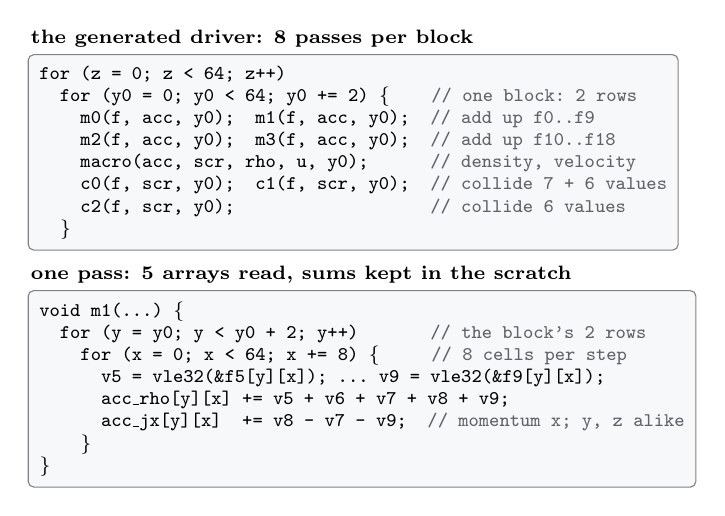
\begin{tikzpicture}
  \node[codebox,anchor=north west] (drv) at (0,0) {%
for\ (z\ =\ 0;\ z\ <\ 64;\ z++)\\
\ \ for\ (y0\ =\ 0;\ y0\ <\ 64;\ y0\ +=\ 2)\ \{\ \ \ \ \textcolor{psgray}{//\ one\ block:\ 2\ rows}\\
\ \ \ \ m0(f,\ acc,\ y0);\ \ m1(f,\ acc,\ y0);\ \ \textcolor{psgray}{//\ add\ up\ f0..f9}\\
\ \ \ \ m2(f,\ acc,\ y0);\ \ m3(f,\ acc,\ y0);\ \ \textcolor{psgray}{//\ add\ up\ f10..f18}\\
\ \ \ \ macro(acc,\ scr,\ rho,\ u,\ y0);\ \ \ \ \ \ \textcolor{psgray}{//\ density,\ velocity}\\
\ \ \ \ c0(f,\ scr,\ y0);\ \ c1(f,\ scr,\ y0);\ \ \textcolor{psgray}{//\ collide\ 7\ +\ 6\ values}\\
\ \ \ \ c2(f,\ scr,\ y0);\ \ \ \ \ \ \ \ \ \ \ \ \ \ \ \ \ \ \ \textcolor{psgray}{//\ collide\ 6\ values}\\
\ \ \}};
  \node[font=\scriptsize\bfseries,anchor=south west,inner sep=1pt] at ([yshift=0.4mm]drv.north west)
    {the generated driver: 8 passes per block};
  \node[codebox,anchor=north west] (pass) at ([yshift=-5mm]drv.south west) {%
void\ m1(...)\ \{\\
\ \ for\ (y\ =\ y0;\ y\ <\ y0\ +\ 2;\ y++)\ \ \ \ \ \ \ \textcolor{psgray}{//\ the\ block's\ 2\ rows}\\
\ \ \ \ for\ (x\ =\ 0;\ x\ <\ 64;\ x\ +=\ 8)\ \{\ \ \ \ \ \textcolor{psgray}{//\ 8\ cells\ per\ step}\\
\ \ \ \ \ \ v5\ =\ vle32(\&f5[y][x]);\ ...\ v9\ =\ vle32(\&f9[y][x]);\\
\ \ \ \ \ \ acc\_rho[y][x]\ +=\ v5\ +\ v6\ +\ v7\ +\ v8\ +\ v9;\\
\ \ \ \ \ \ acc\_jx[y][x]\ \ +=\ v8\ -\ v7\ -\ v9;\ \ \textcolor{psgray}{//\ momentum\ x;\ y,\ z\ alike}\\
\ \ \ \ \}\\
\}};
  \node[font=\scriptsize\bfseries,anchor=south west,inner sep=1pt] at ([yshift=0.4mm]pass.north west)
    {one pass: 5 arrays read, sums kept in the scratch};
\end{tikzpicture}

    \column{0.41\textwidth}
    \vspace{1mm}
    \machine{K1}
    \begin{itemize}\small
      \item Each pass uses at most 7 arrays, so the hardware prefetcher keeps up.
      \item Late cache lines per cell: 1.8 in place, 0.34 with the split loop.
      \item With prefetch added, the split loop was 2 to 13\,\% slower.
    \end{itemize}
  \end{columns}
  \takeaway{So the split build has no prefetch, on both machines.}
\end{frame}

% -----------------------------------------------------------------------------
\subsection{Results}
%  tables/kone-1core-*.dat from board-logs/k1/board/ldc-*-1core.log (presentation4 all.sh, 2026-11-16):
%  best of 3 runs of 200 steps after 10 warm-up, 64^3, one core.
\begin{frame}{K1, one core: throughput of each build}
  \vspace{0mm}
  \centering\onecorefig{kone}{gcc}{clang}{9}{MLUP/s, one core}{2}{}

  \vspace{-1mm}
  {\scriptsize\color{psgray}\machine{K1} Each bar is a separate build; ``with prefetch'' is the build on its left
  plus software prefetch. $64^3$ cells, best of 3 runs of 200 steps (after 10 warm-up steps).\par}
  \todo{Auto-vectorized is as fast as scalar: check why (any vector instructions in the plain kernels?)}
  \takeaway{The split loop is the fastest build: \nv{kone:gcc:f32:1:split} MLUP/s in f32 and
    \nv{kone:gcc:f64:1:split} in f64 (GCC).}
\end{frame}

% -----------------------------------------------------------------------------
\begin{frame}{K1, one core: speedup over plain scalar}
  \vspace{0mm}
  \centering\onecorefig{kone}{gccspd}{clangspd}{6.5}{speedup over plain scalar (same compiler)}{2}{1}

  \vspace{-1mm}
  {\scriptsize\color{psgray}\machine{K1} Each compiler is compared with its own plain scalar build. Same runs as
  before.\par}
  \todo{Auto-vectorized is as fast as scalar: check why (any vector instructions in the plain kernels?)}
  \takeaway{The split loop is \sx{\nv{kone:gcc:f32:1:split/plain}} (f32) and \sx{\nv{kone:gcc:f64:1:split/plain}}
    (f64) as fast as plain scalar. Auto-vectorization changes almost nothing.}
\end{frame}

% -----------------------------------------------------------------------------
\begin{frame}{K1: where the speedup comes from}
  \vspace{1mm}
  {\small Several changes add up. Only one of them is the vector instructions.\par}
  \vspace{2mm}
  \centering
  {\footnotesize\renewcommand{\arraystretch}{1.15}
  \begin{tabular}{@{}lccccrr@{}}
    \toprule
    \textbf{build} & \textbf{CSE} & \textbf{in place} & \textbf{prefetch or split} & \textbf{vectors}
      & \textbf{streams} & \textbf{MLUP/s, f32}\\
    \midrule
    plain scalar & \no & \no & \no & \no & 42 & \nv{kone:gcc:f32:1:plain}\\
    best scalar & \yes & \yes & \no & \no & 23 & \nv{kone:gcc:f32:1:best}\\
    RVV, in place + prefetch & \yes & \yes & prefetch & \yes & 23, prefetched & \nv{kone:gcc:f32:1:aapf}\\
    RVV, split loop & \yes & \yes & split & \yes & at most 7 per pass & \nv{kone:gcc:f32:1:split}\\
    \bottomrule
  \end{tabular}\par}
  \vspace{3mm}
  \raggedright
  \begin{itemize}\small
    \item Prefetch and the split loop both get around the limit of about 20 streams.
    \item The generator applies them only to vector code. So the best scalar build still waits for memory.
  \end{itemize}
  \takeaway{To measure the vectors alone, the scalar build must also stay below 20 streams.
    We do this for both machines at the end.}
\end{frame}

% -----------------------------------------------------------------------------
%  Unchanged from presentation6 (notes5 F6, F18; board-logs/notes5/e6-layout.log in docs/presentation6).
\begin{frame}{K1: the place of the arrays in memory matters}
  \vspace{1mm}
  \centering
  {\footnotesize\renewcommand{\arraystretch}{1.1}
  \begin{tabular}{@{}llrrr@{}}
    \toprule
    \multicolumn{2}{@{}l}{MLUP/s, f32, GCC, one core, two runs}
      & \textbf{default} & \textbf{huge pages} & \textbf{one heap}\\
    \midrule
    periodic box & RVV, in place + prefetch & 7.3 to 7.8 & \textcolor{psred}{3.5 to 3.7} & 7.8 to 7.9\\
                 & RVV, split loop          & 6.3 to 6.4 & 6.2 to 7.3 & 5.6 to 5.9\\
    lid-driven cavity & RVV, in place + prefetch & 6.5 & \textcolor{psred}{4.3 to 7.1} & 6.9\\
                 & RVV, split loop          & 7.6 to 7.7 & 8.0 & 7.6 to 7.7\\
    \bottomrule
  \end{tabular}\par}

  \vspace{3mm}
  \raggedright
  \begin{itemize}\small
    \item Same programs, same results. Only the place of the arrays in memory changes.
    \item With huge pages, the order of the two RVV builds can flip.
  \end{itemize}
  {\scriptsize\color{psgray}\machine{K1} Periodic box: an earlier test case without walls. Huge pages: 2\,MB
  instead of 4\,KB. One heap: all arrays in one memory region. Not tested on the SG2044.\par}
  \takeaway{Small differences between builds are not reliable. Compare builds only with the same memory layout.}
\end{frame}

% -----------------------------------------------------------------------------
\begin{frame}{K1, several cores: total throughput}
  \vspace{-1mm}
  \centering\scalingfig{kone}{0.5}{40}{konescalelegend}

  \vspace{-0.5mm}
  {\scriptsize\ref{konescalelegend}\par}
  \vspace{0.5mm}
  {\scriptsize\color{psgray}\machine{K1} Both axes are logarithmic. Dotted: ideal scaling of the GCC split build.\par}
  \takeaway{From 1 to 8 cores (f32, GCC), the scalar builds gain \sx{\nv{kone:gcc:f32:8:plain/one}} to
    \sx{\nv{kone:gcc:f32:8:best/one}}, the split loop only \sx{\nv{kone:gcc:f32:8:split/one}}.}
\end{frame}

% -----------------------------------------------------------------------------
\begin{frame}{K1, several cores: the RVV advantage shrinks}
  \vspace{0.5mm}
  {\small Each bar shows how many times faster the RVV split loop is than the best scalar build, with the same
  compiler and number of cores. At 1 (dashed line) RVV would gain nothing.\par}
  \vspace{0mm}
  \centering\gainfig{kone}{4.5}{1,4,8}

  \vspace{-0.5mm}
  \raggedright
  {\scriptsize\color{psgray}\machine{K1} Why: on 8 cores the GCC split build moves an estimated
  \nv{kone:gbsk:f32:lo} to \nv{kone:gbsk:f32:hi}\,GB/s during the kernel (f32; f64: \nv{kone:gbsk:f64:lo} to
  \nv{kone:gbsk:f64:hi}\,GB/s). A test loop with the same access pattern reaches about 6\,GB/s.\par}
  \takeaway{RVV is \sx{\nv{kone:gcc:f32:1:split/best}} faster on one core but only \sx{\nv{kone:gcc:f32:8:split/best}}
    on 8 cores (f32, GCC). The 8 cores share one memory, and its bandwidth limits the throughput.}
\end{frame}

% -----------------------------------------------------------------------------
\begin{frame}{K1: where the time goes}
  \vspace{-1mm}
  \centering\timefig{kone}{8}

  \vspace{-1mm}
  {\scriptsize\ref{timelegendkone}\par}
  {\scriptsize\color{psgray}\machine{K1} GCC, best run of each build. The three parts of a time step are explained
  on the slide ``What one time step does''. The wall pass is the same plain C++ code in every build.\par}
  \takeaway{The faster the kernel, the larger the wall pass's share: \nv{kone:share:f32:1:split:wall}\,\% of the
    split build's time on one core (f32).}
\end{frame}

% =============================================================================
\section[Part 2: SG2044]{Part 2: Sophgo SG2044 (128-bit vectors)}
\subsection{The hardware and how we measured}

%  Recon facts (figures/sg2044.tex). MPI: docs/notes7/rvv-vlen128-progress-opus5.5.md, "MPI on monte3".
\begin{frame}{SG2044: the hardware}
  \vspace{0mm}
  \centering% Slide "SG2044: the hardware, and how jobs run". The Sophgo SG2044 on the peak node of Monte Cimone
% (mc-peak-2), as read by scripts/presentation6/recon.sh (recon round 1, 2026-11-20; summary in
% docs/presentation6/presentation6-progress-opus5.5.md, "The machines" and "Round 1"): 64 cores, 1 NUMA node,
% 2.6 GHz; L1 64 KB per core, L2 2 MB per 4 cores, L3 64 MB shared; 124 GB memory (MemTotal); VLEN 128 (vlenb
% register; CMake measures it again in every build: "RISC-V VLEN: 128 bits (measured)"). Core type XuanTie C920v2.
% Cache line 64 B: NOT from recon; from the SG2042 device tree (same XuanTie C920 family, d-cache-block-size =
% <64>); the slide carries a todo until it is read on monte3.
% Nothing else is drawn that recon did not report (no memory latency or bandwidth: not measured on this machine).
% Right: one 128-bit RVV register as 4 f32 or 2 f64 lanes (compare figures/k1.tex: 256 bits, 8 or 4).
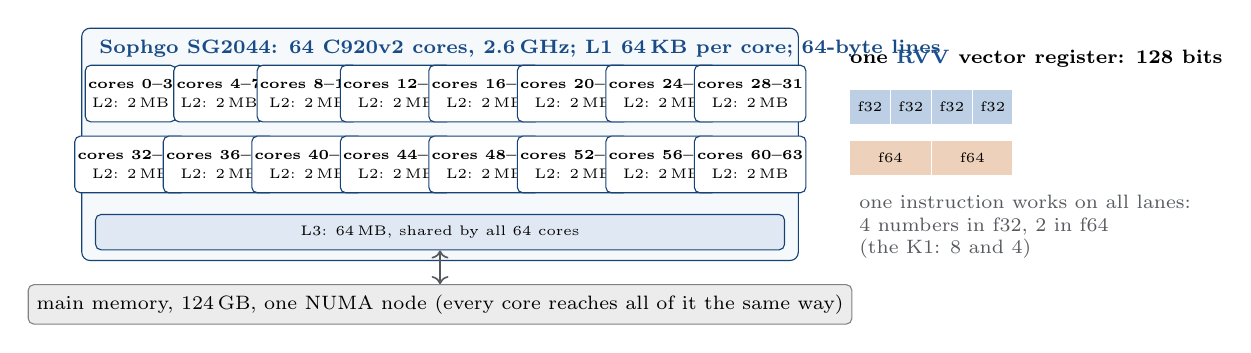
\begin{tikzpicture}[
    cl/.style={box,minimum width=1.02cm,minimum height=0.72cm,fill=white,draw=psblue!70!black,
      font=\tiny,align=center,inner sep=1pt}]
  % ---- the chip: 16 groups of 4 cores ------------------------------------------------
  \draw[psblue!70!black,fill=psblue!4,rounded corners=3pt] (0,0) rectangle (9.1,2.95);
  \node[anchor=north west,font=\scriptsize\bfseries,text=psblue!80!black] at (0.1,2.92)
    {Sophgo SG2044: 64 C920v2 cores, 2.6\,GHz; L1 64\,KB per core; 64-byte lines};
  \foreach \r in {0,1} \foreach \k in {0,...,7} {
    \pgfmathtruncatemacro{\a}{4*(8*\r+\k)}
    \pgfmathtruncatemacro{\b}{\a+3}
    \node[cl] at (0.62+\k*1.124,2.12-\r*0.9) {\textbf{cores \a--\b}\\[1pt]L2: 2\,MB};
  }
  \node[box,fill=psblue!14,draw=psblue!70!black,font=\tiny,minimum height=4.5mm,minimum width=8.75cm,
    inner sep=1pt] (l3) at (4.55,0.36) {L3: 64\,MB, shared by all 64 cores};
  % ---- main memory -------------------------------------------------------------------
  \node[box,fill=psgray!12,minimum width=9.1cm,minimum height=5mm,font=\scriptsize,anchor=north]
    (mem) at (4.55,-0.3) {main memory, 124\,GB, one NUMA node (every core reaches all of it the same way)};
  \draw[<->,semithick,psgray!90!black] (l3.south) -- (l3.south |- mem.north);

  % ---- one core's vector register ------------------------------------------------------
  \begin{scope}[shift={(9.75,0.35)}]
    \def\w{0.52}
    \node[font=\scriptsize\bfseries,anchor=south west,inner sep=0pt] at (0,2.1) {one \term{RVV} vector register: 128 bits};
    \foreach \k in {0,...,3}
      \node[draw=white,line width=0.6pt,minimum height=4.5mm,inner sep=0pt,font=\tiny,fill=psblue!30,
        minimum width=\w cm] at (\k*\w+\w/2,1.6) {f32};
    \foreach \k in {0,...,1}
      \node[draw=white,line width=0.6pt,minimum height=4.5mm,inner sep=0pt,font=\tiny,fill=psorange!30,
        minimum width=2*\w cm] at (\k*2*\w+\w,0.95) {f64};
    \node[lbl,anchor=north west,align=left] at (0,0.6)
      {one instruction works on all lanes:\\4 numbers in f32, 2 in f64\\(the K1: 8 and 4)};
  \end{scope}
\end{tikzpicture}


  \vspace{1mm}
  \raggedright
  \begin{itemize}\small
    \item One node of \term{Monte Cimone}, a RISC-V cluster. Our jobs had the whole node.
    \item MPI: Open MPI 5.0.6. The system's Open MPI 4.1.5 took half of each core's time (backup).
    \item Its list of extensions does not name Zicbop (the K1's does not either). The two prefetch builds contain
          the same prefetch instructions on both machines. Whether the C920v2 acts on them is not tested directly,
          but the in-place build gets faster with them: \nv{sg:gcc:f32:1:aa} $\rightarrow$ \nv{sg:gcc:f32:1:aapf}
          MLUP/s (one core, GCC, f32).
  \end{itemize}
  \takeaway{SG2044: 128-bit vectors, 64 cores, 124\,GB memory.}
\end{frame}

% -----------------------------------------------------------------------------
%  Protocol: scripts/notes7/monte3.sh job-time (job 8566). Checks: slide_data.py.
\begin{frame}{SG2044: how we measured}
  \vspace{1mm}
  \begin{itemize}\small
    \item Every build: 10 warm-up steps, then 60 timed steps. One process per core, 1 to 64 cores.
    \item Three \term{interleaved rounds}: each round runs every build once. We plot the best of the three.
    \item Before each round we check that no core is busy. In \nv{sg:busyrounds} of \nv{sg:rounds} rounds one core
          showed 3\,\% load.
  \end{itemize}
  \vspace{1mm}
  \centering
  {\footnotesize\renewcommand{\arraystretch}{1.12}
  \begin{tabular}{@{}lrr@{}}
    \toprule
    difference between rounds, (best $-$ worst) / best & \textbf{K1} & \textbf{SG2044}\\
    \midrule
    median of all builds and core counts & \nv{kone:spread:median}\,\% & \nv{sg:spread:median}\,\%\\
    configurations above 3\,\% & \nv{kone:spread:nthree} of \nv{kone:spread:n} & \nv{sg:spread:nthree} of \nv{sg:spread:n}\\
    largest, builds shown in the plots & \nv{kone:spread:headline}\,\% & \nv{sg:spread:headline}\,\%\\
    \bottomrule
  \end{tabular}\par}
  \vspace{1mm}
  {\scriptsize\color{psgray}K1: 200 timed steps, 3 runs one after the other. Largest difference of all:
  \nv{sg:spread}\,\% (SG2044, an RVV build that is not in the plots).\par}
  \takeaway{The runs repeat well: half of the configurations vary by less than \nv{sg:spread:median}\,\%.}
\end{frame}

% -----------------------------------------------------------------------------
\subsection{One core}
\begin{frame}{SG2044, one core: throughput of each build}
  \vspace{0mm}
  \centering\onecorefig{sg}{gcc}{clang}{28}{MLUP/s, one core}{1}{}

  \vspace{-1mm}
  {\scriptsize\color{psgray}\machine{SG2044} Each bar is a separate build; ``with prefetch'' is the build on its
  left plus software prefetch. $64^3$ cells, best of 3 rounds of 60 time steps.\par}
  \takeaway{The split loop is the fastest build: \nv{sg:gcc:f32:1:split} MLUP/s in f32 and
    \nv{sg:gcc:f64:1:split} in f64 (GCC). Clang is \nv{sg:clangslower:f32:1:split}\,\% and
    \nv{sg:clangslower:f64:1:split}\,\% slower.}
\end{frame}

% -----------------------------------------------------------------------------
\begin{frame}{SG2044, one core: speedup over plain scalar}
  \vspace{0mm}
  \centering\onecorefig{sg}{gccspd}{clangspd}{5}{speedup over plain scalar (same compiler)}{2}{1}

  \vspace{-1mm}
  {\scriptsize\color{psgray}\machine{SG2044} Each compiler is compared with its own plain scalar build. Same runs as
  before.\par}
  \takeaway{The split loop is \sx{\nv{sg:gcc:f32:1:split/plain}} (f32) and \sx{\nv{sg:gcc:f64:1:split/plain}} (f64)
    as fast as plain scalar, and \sx{\nv{sg:gcc:f32:1:split/best}} and \sx{\nv{sg:gcc:f64:1:split/best}} as fast as
    best scalar (GCC).}
\end{frame}

% -----------------------------------------------------------------------------
%  SG2044 one core: explicit_cse vs explicit_cse_pf, explicit_cse_aa vs explicit_cse_aa_pf (ldc-*-rvv-*-1core.log);
%  output last: share-*-last.log vs share-*-every.log. SWEEPGEN_LDC_OUTPUT=last selects the generated
%  StreamCollide*NoOutput kernels (SweepgenLdcCPU.cpp:169-206), a different kernel per build. The directions
%  stated here are checked by slide_data.py ("statements in the slide text").
\begin{frame}{SG2044, one core: software prefetch}
  \vspace{1mm}
  \centering
  {\footnotesize\renewcommand{\arraystretch}{1.12}
  \begin{tabular}{@{}lrrrr@{}}
    \toprule
    MLUP/s, one core & \multicolumn{2}{c}{\textbf{GCC}} & \multicolumn{2}{c}{\textbf{Clang}}\\
    \cmidrule(lr){2-3}\cmidrule(l){4-5}
    & f32 & f64 & f32 & f64\\
    \midrule
    RVV & \nv{sg:gcc:f32:1:rvv} & \nv{sg:gcc:f64:1:rvv} & \nv{sg:clang:f32:1:rvv} & \nv{sg:clang:f64:1:rvv}\\
    RVV + prefetch & \nv{sg:gcc:f32:1:pf} & \nv{sg:gcc:f64:1:pf} & \nv{sg:clang:f32:1:pf} & \nv{sg:clang:f64:1:pf}\\
    \midrule
    RVV, in place & \nv{sg:gcc:f32:1:aa} & \nv{sg:gcc:f64:1:aa} & \nv{sg:clang:f32:1:aa} & \nv{sg:clang:f64:1:aa}\\
    RVV, in place + prefetch & \nv{sg:gcc:f32:1:aapf} & \nv{sg:gcc:f64:1:aapf} & \nv{sg:clang:f32:1:aapf} & \nv{sg:clang:f64:1:aapf}\\
    \hspace{1em}the same, output only at the end & \nv{sg:aapf:gcc:f32:last} & \nv{sg:aapf:gcc:f64:last}
      & \textcolor{psred}{\nv{sg:aapf:clang:f32:last}} & \textcolor{psred}{\nv{sg:aapf:clang:f64:last}}\\
    \bottomrule
  \end{tabular}\par}
  \vspace{2mm}
  \raggedright
  \begin{itemize}\small
    \item Not in place, prefetch helps Clang but not GCC. In place, it helps both.
    \item \textcolor{psred}{Red}: Clang's in-place + prefetch build reaches only about half the throughput when it writes density
          and velocity only at the end. This happened in all 3 rounds. We have not found the cause yet.
  \end{itemize}
  \takeaway{On the SG2044, prefetch clearly helps only with the in-place update. The split loop is faster than all
    of these builds.}
\end{frame}

% -----------------------------------------------------------------------------
\subsection{Many cores}
\begin{frame}{SG2044, many cores: total throughput}
  \vspace{-1mm}
  \centering\scalingfig{sg}{3}{2000}{sgscalelegend}

  \vspace{-0.5mm}
  {\scriptsize\ref{sgscalelegend}\par}
  \vspace{0.5mm}
  {\scriptsize\color{psgray}\machine{SG2044} Both axes are logarithmic. Dotted: ideal scaling of the GCC split build.\par}
  \takeaway{From 1 to 64 cores (f32, GCC), the scalar builds gain \sx{\nv{sg:gcc:f32:64:plain/one}} to
    \sx{\nv{sg:gcc:f32:64:best/one}}, the split loop only \sx{\nv{sg:gcc:f32:64:split/one}}.}
\end{frame}

% -----------------------------------------------------------------------------
\begin{frame}{SG2044, many cores: throughput per core}
  \vspace{-1mm}
  \centering
  \begin{tikzpicture}
    \begin{groupplot}[res,group style={group size=2 by 1,horizontal sep=4mm,y descriptions at=edge left},coresaxis,ymin=0,ymax=27,height=4.4cm,ylabel={MLUP/s per core},
        legend columns=3,legend style={/tikz/every even column/.append style={column sep=2mm}}]
      \nextgroupplot[title={f32 (single precision)}]
        \addplot[gccline,mark=*] table[x=cores,y=gccplainpc]{tables/sg-scaling-f32.dat};
        \addplot[gccline,mark=square*] table[x=cores,y=gccbestpc]{tables/sg-scaling-f32.dat};
        \addplot[gccline,mark=triangle*,mark size=2.4pt] table[x=cores,y=gccsplitpc]{tables/sg-scaling-f32.dat};
        \addplot[clangline,mark=*] table[x=cores,y=clangplainpc]{tables/sg-scaling-f32.dat};
        \addplot[clangline,mark=square*] table[x=cores,y=clangbestpc]{tables/sg-scaling-f32.dat};
        \addplot[clangline,mark=triangle*,mark size=2.4pt] table[x=cores,y=clangsplitpc]{tables/sg-scaling-f32.dat};
      \nextgroupplot[title={f64 (double precision)},legend to name=sgpclegend]
        \addplot[gccline,mark=*] table[x=cores,y=gccplainpc]{tables/sg-scaling-f64.dat};
        \addplot[gccline,mark=square*] table[x=cores,y=gccbestpc]{tables/sg-scaling-f64.dat};
        \addplot[gccline,mark=triangle*,mark size=2.4pt] table[x=cores,y=gccsplitpc]{tables/sg-scaling-f64.dat};
        \addplot[clangline,mark=*] table[x=cores,y=clangplainpc]{tables/sg-scaling-f64.dat};
        \addplot[clangline,mark=square*] table[x=cores,y=clangbestpc]{tables/sg-scaling-f64.dat};
        \addplot[clangline,mark=triangle*,mark size=2.4pt] table[x=cores,y=clangsplitpc]{tables/sg-scaling-f64.dat};
        \legend{GCC plain scalar,GCC best scalar,GCC RVV split loop,Clang plain scalar,Clang best scalar,Clang RVV split loop}
    \end{groupplot}
  \end{tikzpicture}

  \vspace{-1mm}
  {\scriptsize\ref{sgpclegend}\par}
  {\scriptsize\color{psgray}\machine{SG2044} Flat line = ideal scaling. Estimated memory traffic of the GCC split
  build on 64 cores, during the kernel: \nv{sg:gbsk:f32:lo} to \nv{sg:gbsk:f32:hi}\,GB/s in f32,
  \nv{sg:gbsk:f64:lo} to \nv{sg:gbsk:f64:hi}\,GB/s in f64 (not measured).\par}
  \takeaway{Per core, the split loop drops from \nv{sg:gcc:f32:1:split:percore} to
    \nv{sg:gcc:f32:64:split:percore} MLUP/s (f32). On 64 cores, f32 and f64 move about the same number of bytes per
    second: the memory bandwidth limits the throughput.}
\end{frame}

% -----------------------------------------------------------------------------
\begin{frame}{SG2044, many cores: the RVV advantage shrinks}
  \vspace{0.5mm}
  {\small Each bar shows how many times faster the RVV split loop is than the best scalar build, with the same
  compiler and number of cores. At 1 (dashed line) RVV would gain nothing.\par}
  \vspace{0mm}
  \centering\gainfig{sg}{3}{1,4,8,16,32,64}

  \vspace{-0.5mm}
  \raggedright
  {\scriptsize\color{psgray}\machine{SG2044} The estimated memory traffic on 64 cores is on the previous slide.\par}
  \takeaway{RVV is \sx{\nv{sg:gcc:f32:1:split/best}} faster on one core but only \sx{\nv{sg:gcc:f32:64:split/best}}
    on 64 cores (f32, GCC). The cores share one memory, and its bandwidth limits the throughput.}
\end{frame}

% -----------------------------------------------------------------------------
\begin{frame}{SG2044: where the time goes}
  \vspace{-1mm}
  \centering\timefig{sg}{64}

  \vspace{-1mm}
  {\scriptsize\ref{timelegendsg}\par}
  {\scriptsize\color{psgray}\machine{SG2044} GCC, best run of each build. The three parts are explained on the slide
  ``What one time step does''. The halo exchange includes the time spent waiting for the neighbours.\par}
  \takeaway{On 64 cores the halo exchange takes \nv{sg:share:f32:64:split:comm}\,\% of the split loop's time
    (f32). On one core it takes almost none.}
\end{frame}

% =============================================================================
\section[Both machines]{The two machines compared}
\subsection{The vector gain without the stream limit}

%  cmp: tables/cmp-fair.dat and the fair keys of numbers.tex. K1: board-logs/k1/notes5/e2-A (GCC, 3 rounds),
%  e10-A (Clang, 2 rounds); SG2044: share-*-{every,last}.log (3 rounds). Both: one core, 64^3, interleaved,
%  density and velocity only in the last step (SWEEPGEN_LDC_OUTPUT=last): 19 streams in place.
\begin{frame}{The vector gain without the stream limit}
  \begin{columns}[T,onlytextwidth]
    \column{0.55\textwidth}
    \vspace{-1mm}
    \begin{tikzpicture}
      \begin{groupplot}[res,group style={group size=2 by 1,horizontal sep=3mm,y descriptions at=edge left},
          fairbars,ymin=0,ymax=9,
          symbolic x coords={f32,f64},xtick=data,enlarge x limits=0.5,
          ylabel={speedup: fastest RVV / best scalar},
          nodes near coords={\pgfmathprintnumber[fixed,precision=2,zerofill]{\pgfplotspointmeta}},
          nodes near coords style={font=\tiny,anchor=south,inner sep=1pt},
          clip=false]
        \nextgroupplot[title={K1 (256 bits)}]
          \addplot[gccbar] coordinates {(f32,\nv{kone:fair:gcc:f32}) (f64,\nv{kone:fair:gcc:f64})};
          \addplot[clangbar] coordinates {(f32,\nv{kone:fair:clang:f32}) (f64,\nv{kone:fair:clang:f64})};
          \draw[black!70,thick,densely dashed] ([xshift=-15pt]axis cs:f32,8) -- ([xshift=15pt]axis cs:f32,8)
            node[above,pos=0.5,font=\tiny,text=black!80] {8 lanes};
          \draw[black!70,thick,densely dashed] ([xshift=-15pt]axis cs:f64,4) -- ([xshift=15pt]axis cs:f64,4)
            node[above,pos=0.5,font=\tiny,text=black!80] {4 lanes};
        \nextgroupplot[title={SG2044 (128 bits)},legend style={at={(0.97,0.97)},anchor=north east}]
          \addplot[gccbar] coordinates {(f32,\nv{sg:fair:gcc:f32}) (f64,\nv{sg:fair:gcc:f64})};
          \addplot[clangbar] coordinates {(f32,\nv{sg:fair:clang:f32}) (f64,\nv{sg:fair:clang:f64})};
          \draw[black!70,thick,densely dashed] ([xshift=-15pt]axis cs:f32,4) -- ([xshift=15pt]axis cs:f32,4)
            node[above,pos=0.5,font=\tiny,text=black!80] {4 lanes};
          \draw[black!70,thick,densely dashed] ([xshift=-15pt]axis cs:f64,2) -- ([xshift=15pt]axis cs:f64,2)
            node[above,pos=0.5,yshift=2.5pt,font=\tiny,text=black!80] {2 lanes};
          \legend{GCC,Clang}
      \end{groupplot}
    \end{tikzpicture}
    \column{0.43\textwidth}
    \vspace{1mm}
    \begin{itemize}\small
      \item Here density and velocity are written only in the last step. The in-place loop then has 19 streams
            instead of 23.
      \item So the best scalar build is no longer slowed down by too many streams.
      \item Dashed: the number of lanes, the most that vectors can give.
    \end{itemize}
  \end{columns}
  \vspace{0.5mm}
  {\scriptsize\color{psgray}One core, $64^3$ cells, best of 3 rounds (K1 Clang: 2). The RVV build is the split loop
  (K1 GCC f64: in place + prefetch), so the ratio also includes the effect of its short passes.\par}
  \takeaway{The vectors give \sx{\nv{kone:fair:gcc:f32}} of \sx{8} on the K1 and \sx{\nv{sg:fair:gcc:f32}} of
    \sx{4} on the SG2044 (f32, GCC): far below the number of lanes on both machines.}
\end{frame}

% -----------------------------------------------------------------------------
\subsection{What holds on both machines}
\begin{frame}{What holds on both machines}
  \vspace{1mm}
  \centering
  {\footnotesize\renewcommand{\arraystretch}{1.2}
  \begin{tabular}{@{}lrr@{}}
    \toprule
    GCC, f32 / f64 & \textbf{K1} (256 bits) & \textbf{SG2044} (128 bits)\\
    \midrule
    split loop / best scalar, one core & \sx{\nv{kone:gcc:f32:1:split/best}} / \sx{\nv{kone:gcc:f64:1:split/best}}
      & \sx{\nv{sg:gcc:f32:1:split/best}} / \sx{\nv{sg:gcc:f64:1:split/best}}\\
    split loop / best scalar, all cores & \sx{\nv{kone:gcc:f32:8:split/best}} / \sx{\nv{kone:gcc:f64:8:split/best}}
      & \sx{\nv{sg:gcc:f32:64:split/best}} / \sx{\nv{sg:gcc:f64:64:split/best}}\\
    vector gain without the stream limit & \sx{\nv{kone:fair:gcc:f32}} / \sx{\nv{kone:fair:gcc:f64}}
      & \sx{\nv{sg:fair:gcc:f32}} / \sx{\nv{sg:fair:gcc:f64}}\\
    \hspace{1em}number of lanes & 8 / 4 & 4 / 2\\
    \bottomrule
  \end{tabular}\par}
  \vspace{3mm}
  \raggedright
  \begin{itemize}\small
    \item \textbf{The split loop is the fastest build.} SG2044: in all \nv{sg:ncolumns} cases (2 compilers,
          2 precisions, 6 core counts). K1: in \nv{kone:splitclear} of \nv{kone:ncolumns}; in the other 2 (GCC,
          8 cores) it ties with in place + prefetch.
    \item \textbf{Auto-vectorization does not help.} It is never more than \nv{kone:autovecgain}\,\% (K1) or
          \nv{sg:autovecgain}\,\% (SG2044) faster than scalar. The plain kernels get the distance between
          neighbouring cells only at run time. So the compiler cannot assume that neighbouring cells are next to
          each other in memory.
  \end{itemize}
  {\scriptsize\color{psgray}Each ratio is measured within one machine. Absolute MLUP/s are not compared: the
  sessions, step counts and Clang versions differ.\par}
  \takeaway{The same picture on both machines: the split loop wins, the vectors give far less than their lane count,
    and the gain shrinks when all cores share the memory.}
\end{frame}

% =============================================================================
\section{Summary}

\begin{frame}{Summary}
  \vspace{2mm}
  \begin{itemize}
    \item \textbf{One generator, two widths.} pystencils and waLBerla generate RVV code for 128 or 256 bits.
          The build measures the width. A mismatch stops the build.
    \item \textbf{Correct.} All 44 programs on each machine match the reference solution.
    \item \textbf{Faster on one core.} \sx{\nv{kone:gcc:f32:1:split/plain}} (K1) and
          \sx{\nv{sg:gcc:f32:1:split/plain}} (SG2044) over plain scalar code (f32, GCC).
      \begin{itemize}
        \item About \sx{2} from the vectors, the rest from CSE and fewer streams.
      \end{itemize}
    \item \textbf{Limited by memory on all cores.} \sx{\nv{kone:gcc:f32:8:split/best}} (K1) and
          \sx{\nv{sg:gcc:f32:64:split/best}} (SG2044) over the best scalar build.
  \end{itemize}
\end{frame}

% -----------------------------------------------------------------------------
\begin{frame}{Open questions}
  \vspace{2mm}
  \begin{itemize}
    \item Why does Clang's in-place + prefetch build reach only half the throughput on the SG2044 when it writes its output only
          at the end?
    \item Does the SG2044's core execute the prefetch hint? A stream test like the one on the K1 would tell.
    \item Tuning for each chip: register grouping (LMUL), prefetch distance, size of the split passes. The generator
          has these options, but we have not tested them yet.
    \item Does the memory layout (huge pages) matter on the SG2044 as it does on the K1?
  \end{itemize}
\end{frame}

% -----------------------------------------------------------------------------
\begin{frame}{Code, data and acknowledgement}
  \vspace{1mm}
  \small
  \begin{tabularx}{\textwidth}{@{}l l X@{}}
    \toprule
    Repository & Branch, commit & Contents\\
    \midrule
    \href{https://github.com/salehjg/mirrored-pystencil2/tree/rvv-support}{\code{mirrored-pystencil2}}
      & \code{rvv-support}, \code{78afe1ff} & pystencils: RVV targets for 128 and 256 bits, prefetch\\
    \href{https://github.com/salehjg/mirrored-walberla/tree/rvv-support}{\code{mirrored-walberla}}
      & \code{rvv-support}, \code{42855054} & waLBerla: width probe, flags, in-place update, the benchmark\\
    \href{https://github.com/salehjg/my-e4-ws}{\code{my-e4-ws}} & \code{main}, \todo{the commit with docs/presentation7-v2}
      & workspace: both forks, scripts, K1 logs, these slides\\
    \bottomrule
  \end{tabularx}

  \vspace{4mm}
  {\small\bfseries Acknowledgement\par}
  {\footnotesize The SG2044 results were obtained on the Monte Cimone RISC-V cluster. We thank the Monte Cimone
  project for access. Reference: DOI \href{https://doi.org/10.1007/978-3-032-07612-0_44}{10.1007/978-3-032-07612-0\_44}.\par}
  \vfill
  \centering{\Huge\bfseries\color{psred}Thank you\par}
  \vspace{2mm}
\end{frame}

% =============================================================================
\appendix
\section{Backup}

\begin{frame}{Glossary (1/3)}
  \begin{columns}[T,onlytextwidth]
    \column{0.49\textwidth}
    \scriptsize
    \begin{description}\setlength{\itemsep}{0.8pt}
      \item[AA pattern] in-place update: one array (A) is read and written; even and odd steps alternate.
      \item[AB pattern] the usual update: read array A, write array B, then swap them.
      \item[Auto-vectorization] the compiler turns a plain loop into vector code by itself.
      \item[Backend] the part of pystencils that writes code for one instruction set (x86, ARM, RVV, \ldots).
      \item[Best scalar build] no vector instructions, but with CSE and the in-place update.
      \item[Block] a box of cells; waLBerla cuts the domain into blocks, here one per process.
      \item[Bounce-back] the wall rule: a value that would flow into the wall comes back in the opposite direction.
      \item[C920v2] the XuanTie core type of the SG2044.
      \item[Cache line] the unit in which memory moves to the cache: 64 bytes on both machines, i.e.\ 16 f32 or 8 f64 values.
      \item[Cache miss] the data is not in the cache and must come from main memory.
    \end{description}
    \column{0.49\textwidth}
    \scriptsize
    \begin{description}\setlength{\itemsep}{0.8pt}
      \item[CSE] common subexpression elimination: each repeated part of a formula is computed once.
      \item[D3Q19] the LBM model used here: 3 dimensions, 19 directions per cell.
      \item[Density $\rho$] the amount of fluid in a cell; computed from its 19 values.
      \item[Energy] here: the sum of $u_x^2+u_y^2+u_z^2$ over all cells, printed at the end of each run.
      \item[$f_i$, $f'_i$] the 19 values of a cell before ($f_i$) and after ($f'_i$) a time step; each has its own array.
      \item[f32, f64] single (32-bit) and double (64-bit) precision floating-point numbers.
      \item[GCC, Clang] the two C++ compilers we compare.
      \item[Ghost layer] a one-cell layer around each block that holds copies of the neighbour's border cells.
      \item[Halo exchange] the update of the ghost layers after each time step.
      \item[Hardware prefetcher] a part of the cache that detects regular access patterns and loads data early.
    \end{description}
  \end{columns}
\end{frame}

\begin{frame}{Glossary (2/3)}
  \begin{columns}[T,onlytextwidth]
    \column{0.49\textwidth}
    \scriptsize
    \begin{description}\setlength{\itemsep}{0.8pt}
      \item[Hint] an instruction that cores without the extension run as an instruction that does nothing.
      \item[Huge page] a 2\,MB page of memory instead of 4\,KB.
      \item[In order] a core that runs instructions strictly in program order, so it waits for each missing value.
      \item[Interleaved rounds] each round runs every build once, so slow changes affect all builds alike.
      \item[Intrinsic] a C/C++ function that the compiler turns into one machine instruction.
      \item[K1, X60] the SpacemiT chip on the board, and its core type.
      \item[Kernel] the generated loop that updates all cells once.
      \item[Lane] the slot of one number in a vector register.
      \item[Layout fzyx] waLBerla's memory order: $x$ fastest, then $y$, then $z$; each value $f_i$ has its own array.
      \item[LBM] lattice Boltzmann method: a fluid simulation on a grid of cells.
    \end{description}
    \column{0.49\textwidth}
    \scriptsize
    \begin{description}\setlength{\itemsep}{0.8pt}
      \item[lbmpy] a Python package that derives the LBM formulas for one cell.
      \item[Lid-driven cavity] a closed box whose top wall moves: a standard flow test case.
      \item[MLUP/s] million cell updates per second: the unit of throughput.
      \item[Monte Cimone] a RISC-V cluster; one of its nodes has the SG2044.
      \item[MPI] the standard library for messages between processes; Open MPI is one implementation.
      \item[Periodic box] an earlier test case without walls: what leaves one side comes back on the other.
      \item[Plain scalar build] the same program compiled without any vector instructions.
      \item[pystencils] a Python package that turns formulas into a C++ loop over all cells.
      \item[RISC-V] an open instruction set architecture.
      \item[RVV] the RISC-V vector extension.
    \end{description}
  \end{columns}
\end{frame}

\begin{frame}{Glossary (3/3)}
  \begin{columns}[T,onlytextwidth]
    \column{0.49\textwidth}
    \scriptsize
    \begin{description}\setlength{\itemsep}{0.8pt}
      \item[SG2044] the Sophgo chip with 64 cores used in part 2.
      \item[sha256] a checksum of a file: the same file always gives the same value. Here: of each benchmark executable.
      \item[Software prefetch] an instruction that asks the cache to load data that will be needed soon.
      \item[Split loop] the cell update in 8 short passes, each with few arrays.
      \item[Stall] a cycle in which the core cannot continue, because it waits for data or for a result.
      \item[Stencil] the set of cells needed to update one cell; here 19 (D3Q19).
      \item[Stream] a run of consecutive cache lines that a loop walks through in order, for example one array.
      \item[Stride] the address distance between two neighbouring cells of a loop.
      \item[Target] tells pystencils which backend and options to use, e.g.\ \code{RISCV\_RVV128}.
      \item[Throughput] cell updates per second, in MLUP/s; a speedup is a ratio of two throughputs.
    \end{description}
    \column{0.49\textwidth}
    \scriptsize
    \begin{description}\setlength{\itemsep}{0.8pt}
      \item[Velocity $u$] the speed and direction of the fluid in a cell, with parts $u_x$, $u_y$, $u_z$.
      \item[vl] vector length: how many numbers one RVV instruction handles.
      \item[VLEN] the width of a chip's vector registers in bits: 256 (K1), 128 (SG2044).
      \item[waLBerla] an open-source C++ framework for fluid simulations.
      \item[Wall pass] the third part of a time step: applies bounce-back to the cells next to a wall; plain C++ in every build.
      \item[Weak scaling] more cores, a larger domain, the same work per core.
      \item[Write-allocate] before a store, the cache first loads the line from memory.
      \item[Zicbop] the RISC-V extension with prefetch instructions.
    \end{description}
  \end{columns}
\end{frame}

% -----------------------------------------------------------------------------
%  Full tables: tables/<machine>-table-<prec>.tex (slide_data.py), best MLUP/s, all cores together.
\newcommand{\fulltable}[4]{% #1 machine, #2 precision, #3 core count header cells, #4 number of core counts
  \CatchFileDef{\fulltablerows}{tables/#1-table-#2.tex}{}%
  {\scriptsize\renewcommand{\arraystretch}{1.02}\setlength{\tabcolsep}{3.2pt}
  \begin{tabular}{@{}l*{#4}{r}*{#4}{r}@{}}
    \toprule
    & \multicolumn{#4}{c}{\textbf{GCC}, cores} & \multicolumn{#4}{c}{\textbf{Clang}, cores}\\
    \cmidrule(lr){2-\the\numexpr #4+1\relax}\cmidrule(l){\the\numexpr #4+2\relax-\the\numexpr 2*#4+1\relax}
    MLUP/s, #2 & #3 & #3\\
    \midrule
    \fulltablerows
    \bottomrule
  \end{tabular}\par}}

\begin{frame}{Numbers: K1, every build, f32}
  \centering
  \fulltable{kone}{f32}{1 & 4 & 8}{3}

  \vspace{2mm}
  \raggedright
  {\scriptsize\color{psgray}\machine{K1} Best of 3 runs of 200 steps, $64^3$ cells per core, all cores together.
  Bold: the fastest build of the column. GCC~14.2, Clang~18.1.\par}
\end{frame}

\begin{frame}{Numbers: K1, every build, f64}
  \centering
  \fulltable{kone}{f64}{1 & 4 & 8}{3}

  \vspace{2mm}
  \raggedright
  {\scriptsize\color{psgray}\machine{K1} As in the f32 table.\par}
\end{frame}

\begin{frame}{Numbers: SG2044, every build, f32}
  \centering
  \fulltable{sg}{f32}{1 & 4 & 8 & 16 & 32 & 64}{6}

  \vspace{2mm}
  \raggedright
  {\scriptsize\color{psgray}\machine{SG2044} Best of 3 interleaved rounds of 60 steps, $64^3$ cells per core, all
  cores together. Bold: the fastest build of the column. GCC~14.2, Clang~17.\par}
\end{frame}

\begin{frame}{Numbers: SG2044, every build, f64}
  \centering
  \fulltable{sg}{f64}{1 & 4 & 8 & 16 & 32 & 64}{6}

  \vspace{2mm}
  \raggedright
  {\scriptsize\color{psgray}\machine{SG2044} As in the f32 table.\par}
\end{frame}

% -----------------------------------------------------------------------------
%  docs/notes7/rvv-vlen128-progress-opus5.5.md, "MPI on monte3" (jobs 8552, 8555, 8559-8564) and the timing job's
%  MPI check (mpi-<N>.log of run 20261122-214637: halo pattern, 64 KiB, 20 repeats).
\begin{frame}{SG2044: the MPI problem and the fix}
  \vspace{1mm}
  \centering
  {\footnotesize\renewcommand{\arraystretch}{1.15}
  \begin{tabular}{@{}lll@{}}
    \toprule
    & \textbf{system Open MPI 4.1.5} & \textbf{Open MPI 5.0.6 (module)}\\
    \midrule
    helper thread in each process & busy (100\,\%), shares the core & idle (0\,\%)\\
    ring exchange of 1\,KiB / 64\,KiB, 4 processes & 10\,000\,$\mu$s / 30\,000\,$\mu$s & 9.6\,$\mu$s / 209\,$\mu$s\\
    hangs & 16-process run; all-to-all test & none (2 to 64 processes)\\
    \bottomrule
  \end{tabular}\par}
  \vspace{3mm}
  \raggedright
  \begin{itemize}\small
    \item With one core per process, the busy helper thread took half of each core, and every message waited
          about 10\,ms for its turn. We discarded those timings and rebuilt everything with 5.0.6.
    \item The timing job checks MPI before each core count: \nv{sg:mpihalo:4}\,$\mu$s (4 processes) to
          \nv{sg:mpihalo:64}\,$\mu$s (64 processes) per halo-like exchange of 64\,KiB, every byte correct.
  \end{itemize}
  \takeaway{All SG2044 numbers in this talk come from one session with Open MPI 5.0.6.}
\end{frame}

% -----------------------------------------------------------------------------
\begin{frame}{How the results are checked, in detail}
  \vspace{1mm}
  \begin{itemize}\small
    \item \textbf{Reference cases}: 1 process with $16^3$ cells at 100 and 101 steps (the in-place builds alternate
          between even and odd steps), 2 processes with $32\times16\times16$, 6 processes with $16\times24\times8$.
          Per build: largest difference of density and velocity, mass, mirror symmetry.
    \item \textbf{Decomposition}: $32^3$ cells on 1 process against 8 processes with $16^3$: bit for bit.
    \item \textbf{Compilers}: GCC against Clang on every reference case.
    \item \textbf{Builds}: every compile line has the expected \code{-march} and \code{-O3}; scalar programs contain no
          vector instructions; RVV kernels do; on the SG2044 every program uses Open MPI 5.0.6.
    \item \textbf{Timed runs}: the sha256 of each program must be in the verification log; every run of a build ends
          with the same field hash; the 11 builds agree in energy.
    \item \textbf{Same code at 256 bits}: the K1 runs used the generator from before the 128-bit work. At 256 bits
          the new generator writes the same code (byte for byte for the in-place + prefetch and split builds,
          pystencils' tests for the others).
  \end{itemize}
  \vfill
  {\scriptsize\color{psgray}\code{scripts/presentation7/slide\_data.py} repeats these checks for the slides and
  stops if any fails. It also checks every statement about the data in the slide text. Not tested: box sizes that
  are not a multiple of the vector length.\par}
\end{frame}

\end{document}
